%start% Brought this in from Patrick thesis
\documentclass{thesis}
\usepackage[utf8]{inputenc}
\usepackage{parskip}
\usepackage{hepnames}
% \usepackage[printonlyused]{acronym}
\usepackage{thesis}
\usepackage{ptdr-definitions}
\usepackage{hepnicenames}
\usepackage{hepunits}
\usepackage{abhep}
\usepackage{slashed}
\usepackage{multirow}
%end%
%\documentclass[hyperpdf]{hepthesis}
%\documentclass[a4paper,10pt]{book}
%\usepackage{fullpage}
%\usepackage[margin=2cm]{geometry} % Defining geometry of the usable text space

%% Using Babel allows other languages to be used and mixed-in easily
%\usepackage[ngerman,english]{babel}
% \usepackage[english]{babel}
% \selectlanguage{english}

%% Citation system tweaks
% \usepackage{cite}

% \usepackage{amsmath}
% \usepackage{amsthm}
% \usepackage{amsfonts}
% \usepackage{amssymb}
% \usepackage{graphicx}
% \usepackage{color}                 % For color (highlights,...) 
% \usepackage{caption}               % ?????
% \usepackage{soul}                  % For text highlights
\usepackage{threeparttable}        % Better tables
% \usepackage{hyperref}              % Need after glossaries (allows links)
\usepackage[toc,acronym]{glossaries} %(recommended) for the indexing phase, as opposed to makeindex (the default)
\makeglossaries
% \newacronym[longplural={Frames per Second}]{fpsLabel}{FPS}{Frame per Second}

%A
\newacronym{ALICE}{ALICE}{A Large Ion Collider Experiment}
\newacronym{ATLAS}{ATLAS}{A Toroidal LHC ApparatuS}
\newacronym{APD}  {APD}  {Avalanche photo-diodes}

%B
\newacronym{BSM}{BSM}{Beyond the Standard Model}
\newacronym{BDT}{BDT}{Boosted Decision Tree}

%C
\newacronym{CERN}{CERN}{European Organization for Nuclear Research} %derived from the name Conseil Européen pour la Recherche Nucléaire
\newacronym{CMS} {CMS} {Compact Muon Solenoid}

%D
\newacronym{DAQ}{DAQ}{Data Acquisition}
\newacronym{DQM}{DQM}{Data Quality Monitoring}

%E
\newacronym{EB}  {EB}  {ECAL Barrel}
\newacronym{EE}  {EE}  {ECAL Endcap}
\newacronym{ECAL}{ECAL}{Electromagnetic Calorimeter}

%F
\newacronym{FCT}{FCT}   {Fundação para a Ciência e a Tecnologia}

%G

%H
\newacronym{HCAL}{HCAL}  {Hadronic Calorimeter}
\newacronym{HLT} {HLT}   {High Level Trigger}

%I

%J
\newacronym{JER}{JER}{jet energy resolution}
\newacronym{JES}{JES}{jet energy scale}

%K

%L
\newacronym{L1T}   {L1T}   {Level 1 Trigger}
\newacronym{LINAC2}{LINAC2}{Linear Particle Accelerator 2}
\newacronym{LHC}   {LHC}   {Large Hadron Collider}

%M
\newacronym{MC} {MC} {Monte Carlo}
\newacronym{MET}{MET}{Missing Transverse Energy}

%N

%O

%P
\newacronym{PS} {PS} {Proton Synchrotron}
\newacronym{PSB}{PSB}{Proton Synchrotron Booster}

%Q

%R

%S
\newacronym{SM} {SM} {Standard Model}
\newacronym{SPS}{SPS}{Super  Proton Synchrotron}

%T

%U

%V
\newacronym{VBF}{VBF}{vector Boson Fusion}
\newacronym{VPT}{VPT}{Vacuum Photo-Triodes}
%W

%X

%Y

%Z


% \acro{CL}{confidence level}
% \acro{CSC}{cathode strip chamber}
% \acro{CSV}{combined secondary vertex}
% \acro{CTF}{combinatorial track finder}
% \acro{DA}{deterministic annealing}
% \acro{DT}{drift tube}
% \acro{GSF}{Gaussian sum filter}
% \acro{HB}{hadron barrel}
% \acro{HE}{hadron endcaps}
% \acro{HF}{hadron forward}
% \acro{HLT}{high-level trigger}
% \acro{HO}{hadron outer}
% \acro{HPS}{hadron plus strips}
% \acro{JER}{jet energy resolution}
% \acro{JES}{jet energy scale}
% \acro{L1}{Level-1}
% \acro{LHCHXSWG}{LHC Higgs Cross Section Working Group}
% \acro{LO}{leading order}
% \acro{MPF}{missing transverse energy projection fraction}
% \acro{MPI}{multi-parton interaction}
% \acro{MVA}{multi-variate analysis}
% \acro{MSSM}{minimal supersymmetric standard model}
% \acro{NLO}{next-to-leading order}
% \acro{NNLO}{next-to-next-to-leading order}
% \acro{NNLL}{next-to-next-to-leading logarithmic}
% \acro{pdf}{probability density function}
% \acro{PDF}{parton distribution function}
% \acro{PF}{particle flow}
% \acro{PS}{Proton Synchrotron}
% \acro{PSB}{Proton Synchrotron Booster}
% \acro{PU}{pile-up}
% \acro{PV}{Primary Vertex}
% \acro{QCD}{Quantum Chromodynamics}
% \acro{RF}{radio frequency}
% \acro{RPC}{resistive plate chamber}
% \acro{SPS}{Super Proton Synchrotron}
% \acro{SSV}{simple secondary vertex}
% \acro{SM}{standard model}
% \acro{TEC}{tracker endcaps}
% \acro{TIB}{tracker inner barrel}
% \acro{TID}{tracker inner disks}
% \acro{TOB}{tracker outer barrel}
% \acro{UE}{underlying event}
% \acro{VBF}{vector boson fusion}
% \acro{WLCG}{Worldwide LHC Computing Grid}


% DEBUG: Adding line numbers
\linenumbers

\title{Search for Higgs Decay to Dark Matter and Trigger Studies} 
\author{João Carlos Arnauth Pela}
% \email[Contact email: ]{joaopela@gmail.com}
% \affiliation{Imperial College London}
% \keywords{Particle Physics}
\date{21 September 2015}


%% Doc-specific PDF metadata
\makeatletter
\@ifpackageloaded{hyperref}{
\hypersetup{
  pdftitle    = {Search for Higgs Decay to Dark Matter and Trigger Studies},
  pdfsubject  = {João Pela's PhD thesis},
  pdfkeywords = {LHC, CMS, Higgs, Dark Matter, Trigger},
  pdfauthor   = {\textcopyright\ João Pela}
}
}{}
\makeatother

\begin{document}

\begin{frontmatter}
  %% Title
%!!UPDATE THIS
\titlepage[of Imperial College London]%
{A dissertation submitted to Imperial College London\\
  for the degree of Doctor of Philosophy}
  
\clearpage
\textbf{The copyright of this thesis rests with the author and is made available under a Creative Commons 
Attribution Non-Commercial No Derivatives licence. Researchers are free to copy, distribute or 
transmit the thesis on the condition that they attribute it, that they do not use it for commercial 
purposes and that they do not alter, transform or build upon it. For any reuse or redistribution, 
researchers must make clear to others the licence terms of this work.}


%% Abstract
\begin{abstract}%[\smaller \thetitle\\ \vspace*{1cm} \smaller {\theauthor}]
The Compact Muon Solenoid (CMS) is a general-purpose particle detector at the CERN Large Hadron Collider (LHC). The goal of this experiment is to search for the Higgs boson and evidence of new physics and to test the prediction of the Standard Model (SM) at the TeV scale. This thesis describes the analysis of proton-proton collision data recorded by CMS during 2012 and support work for data taking during the same period.

A search for the Vector Boson Fusion (VBF) produced Higgs boson invisible decays, using $19.5\,\femto\barn^-1$ of data recorded with prompt reconstruction triggers at a center of mass energy of $8\,\TeV$, is presented. Events are selected with two forward jets and large Missing Transverse Momentum. Assuming the SM VBF production cross section and acceptance, the observed (expected) upper limit at the 95\% confidence level on the \BRinv\, is determined to be of 65\% (49\%) for $m_H=125\,\GeV$.

A second search for the VBF Higgs boson invisible decays, using $19.2\,\femto\barn^-1$ of data recorded with delayed reconstruction (parked) triggers at a center of mass energy of $8\,\TeV$, is also presented. A new event selection criteria was developed taking advantage of the lower trigger requirements. Assuming the SM VBF Higgs production cross section and acceptance, the observed (expected) upper limit at the 95\% confidence level on the \BRinv\, is determined to be of 57\% (40\%) for $m_H=125\,\GeV$.

Monitoring for the CMS Level 1 Trigger system has been developed and used during the 2012 and subsequent LHC data acquisition periods. Contribution to the high reliability of this system during data taking and providing crucial information for validation of the data quality.
\end{abstract}

%DONE

%% Declaration
\begin{declaration}
I declare that the work contained in this thesis is my own, and all results and figures taken from other sources are indicated in the text and referenced appropriately. The analyses presented in this thesis were developed in close collaboration with other members of the CMS experiment.

For the Vector Boson Fusion (VBF) Higgs to invisible prompt analysis I have contributed with the literature review and final background cross section input values for background normalization. QCD multi-jet background studies were also preformed with the target of improving the final selection or prepare the parked analysis, this analysis is presented to give context for the more important work developed later. 

For the VBF Higgs to invisible parked analysis I have participated in the development of the parked trigger, which was used to record the majority of the analysed data. I have continued the QCD multi-jet background studies which have lead to the production of dedicated Monte Carlo simulations and novel approaches to reject this type of events. I have been the responsible for the cross check analysis of the main result which has successfully validated the implementation of the main analysis \cite{ARTICLE:CMSVBFHiggsInvisibleParkedAnalysisPAS}. It is a normal a requirement for many \gls{CMS} publications to have a cross check analysis implemented independently from the main result in order to be able to ensure the accuracy of the final results. I have also participated in the preparation of the Run II analysis where I have lead the development of both the triggers used for data recording during 2015. Additionally, I have developed a method to create the first QCD multi-jet Monte Carlo sample with no MET requirements with signal like properties.

As part of the CMS Level 1 Trigger (L1T) Detector Performance Group (DPG) I have developed monitoring tools for this system, which were both used for real-time monitoring and posterior data certification for physics analysis usage. My work in this group has lead to my appointment for two years to the position of coordinator of the \gls{CMS} \gls{L1T} Data quality Monitoring software development team. Field work was also performed by doing shifts as Trigger and Shift Leader in the experiment control room and on call shifts as the Trigger Detector on Call (DOC) expert.
 
\vspace*{1cm}
\begin{flushright}
João Pela
\end{flushright}
\end{declaration}

%% Acknowledgements
\begin{acknowledgements}
I would like to thank the Imperial College HEP Group and the FCT for supporting and giving me the opportunity to pursue research including my time spent at CERN. Thanks to my supervisor, David Colling, for his guidance during the years of my PhD, the many useful discussions and his enthusiasm for particle physics research. Thanks must also go to all my colleagues of the CMS VBF Higgs to invisible group with whom I have worked directly, Patrick Dunne, Anne-Marie Magnan, Alexandre Nikitenko, Jim Brooke and Chayanit Asawatangtrakuldee. Thanks to everyone in CMS L1T DPG group, specially to Carlo Battilana and Arno Heister for their support. Thanks to all my friends that supported me on my way to finish this degree, it is difficult to mention all of you, but here is a small list, Antonio Pacheco, André David, Alice Mitchell, Chris Holdsworth-Swan, Francisco Sousa, Glenn Spiers, Guillermo Marrero, João Filipe, Miguel Cunhal, Miguel Machado, Nadia Silva, Raquel Monteiro, and many, many more. Finally, and most importantly, I thank my parents and grandparents for their constant support, love and encouragement.
\end{acknowledgements}

\clearpage

\vspace*{\fill}
The work presented in this thesis was supported by the Portuguese Government through \gls{FCT} in the form of my PhD grant with the reference SFRH/BD/77979/2011. I am thankful for their support which allowed me to attain higher education.
\vspace*{\fill}

\begin{center}
\resizebox{1.0\linewidth}{!}{

\includegraphics{FrontMatter/Images/FundingBand.png}
}
\end{center}


% \begin{preface}
% Thesis structure and so on...
% \end{preface}

\dedication{To my grandmother.}

%% Preface
%\begin{preface}
%\end{preface}

%% ToC
\tableofcontents

\newpage
\listoffigures

\newpage
\listoftables

%% Strictly optional!
%\frontquote%
%{Writing in English is the most ingenious torture\\
%   ever devised for sins committed in previous lives.}%
%  {James Joyce}
 
% \titlepage[of the High Energy Physics Group]{%
%   A dissertation submitted to the Imperial College London\\ for the degree of Doctor of Philosophy}

\end{frontmatter}

\begin{mainmatter}
  \chapter{Theory}
%NOTE: Maybe would be good to make a more descriptive title

\colorbox{red}{
\begin{minipage}{0.95\linewidth}
TODO: 
\begin{itemize}
  \item Global status
\end{itemize}

\end{minipage}
}

\section{Standard Model of Particle Physics}

\colorbox{red}{
\begin{minipage}{0.95\linewidth}
TODO: 

\begin{itemize}
  \item Very brief summary of the Standard Model.
\end{itemize}

\end{minipage}
}

The \gls{SM} of particle physics is the currently accepted model for describing the physics of elementary particles.

\begin{table}[!htb]
  \centering
  \begin{tabular}{|c|c|c|c|c|}
  \hline
  \multicolumn{5}{|c|}{Leptons (J=1/2)} \\
  \hline
  Generation & Particle Name & Symbol & Mass ($GeV/c^2$) & Q/e \\
  \hline
  \hline
  \multirow{2}{*}{$1^{st}$} & Electron          & e          &           0.000511    & 1 \\
                            & Electron Neutrino & $\nu_e$    & $< 3 \times 10^-9$    & 0 \\
  \hline
  \hline
  \multirow{2}{*}{$2^{nd}$} & Muon              & $\mu$      &              0.106    & 1 \\
                            & Muon Neutrino     & $\nu_\mu$  & $< 1.9 \times 10^-4$  & 0 \\
  \hline
  \hline
  \multirow{2}{*}{$3^{rd}$} & Tau               & $\tau$     & 1.777                 & 1 \\
                            & Tau Neutrino      & $\nu_\tau$ & $< 1.82 \times 10^-2$ & 0 \\
  \hline
  \end{tabular}
  \caption[List of leptons and their fundamental properties]{List of leptons and their fundamental properties}
  \label{TheoreticalIntroduction_LeptonProperties}
\end{table}

\begin{table}[!htb]
  \centering
  \begin{tabular}{|c|c|c|c|c|}
  \hline
  \multicolumn{5}{|c|}{Quarks (J=1/2)} \\
  \hline
  Generation & Particle Name & Symbol & Mass ($GeV/c^2$) & Q/e \\
  \hline
  \hline
  \multirow{2}{*}{$1^{st}$} & Up      & u & $1.5-3.3 \times 10^{-3}$ & -2/3 \\
                            & Down    & d &   $3.5-6 \times 10^{-3}$ &  1/3 \\
  \hline
  \hline
  \multirow{2}{*}{$2^{nd}$} & Charm   & c &                1.16-1.34 & -2/3 \\
                            & Strange & s &  $70-130 \times 10^{-3}$ &  1/3 \\
  \hline
  \hline
  \multirow{2}{*}{$3^{rd}$} & Top     & t &                  169-173 & -2/3 \\
                            & Bottom  & b &              $4.13-4.37$ &  1/3 \\
  \hline
  \end{tabular}
  \caption[List of quarks and their fundamental properties]{List of quarks and their fundamental properties}
  \label{TheoreticalIntroduction_QuarkProperties}
\end{table}

\begin{table}[!htb]
  \centering
  \begin{tabular}{|c|c|c|c|c|}
  \hline
  \multicolumn{4}{|c|}{Bosons} \\
  \hline
   Particle Name & Mass ($GeV$) &     Q/e & Spin \\
  \hline
  \hline
  Photon ($\gamma$) &                  0 &       0 &    1 \\
  \hline
  $W^\pm$           & $80.385 \pm 0.015$ & $\mp 1$ &    1 \\
  $Z^0$             & $91.1876\pm0.0021$ &       0 &    1 \\
  \hline
  Gloun (g)         &                  0 &       0 &    1 \\
  \hline
  \end{tabular}
  \caption[List of bosons and their fundamental properties]{List of force carrying bosons and their fundamental properties \cite{ARTICLE:PDG2014}.}
  \label{TABLE:Theory_SM_ParticlesAndForces_BosonProperties}
\end{table}


\section{Higgs Mechanism}

Summary of the Higgs Mechanism. Should include
\begin{itemize}
 \item Motivations 
 \item Explanation of the mechanism itself
 \item Consequences 
 \item Possible decays
\end{itemize}

\section{Higgs Invisible decays}

\colorbox{red}{
\begin{minipage}{0.95\linewidth}
TODO: 
\begin{itemize}
  \item Explain what are SM Higgs invisible decays.
  \item Go over the possibility of BSM invisible decays.
\end{itemize}

\end{minipage}
}


  \chapter{Experimental Apparatus}
\label{CHAPTER:ExperimentalApparatus}

\glsresetall % Resetting all acronyms

%%%%%%%%%%%%%%%%%%%%%%%%%%%%%%%%%%%%%%%%%%%%%%%%%%%%%%%%%%%%%%%%%%%%%%%%%%%%%%%%%%%%%%%
%%% SECTION
%%%%%%%%%%%%%%%%%%%%%%%%%%%%%%%%%%%%%%%%%%%%%%%%%%%%%%%%%%%%%%%%%%%%%%%%%%%%%%%%%%%%%%%
\section{The Large Hadron Collider}
\label{SECTION:ExperimentalApparatus_LHC}

% Status: DONE (reviewed J.Pela x1)
%
% TODO:
% * DONE: LHC location, size, particles used, energy usage.
% * Basics of machine and operation
% * How instantaneous luminosity is calculated include Instantaneous luminosity equation
% * Delivered instantaneous luminosity Run I (proton-Proton)

% \colorbox{red}{
% \begin{minipage}{0.95\linewidth}
%  
% \begin{itemize}\item\end{itemize}
% \end{minipage}
%}

% CERN and LHC Location
The \gls{LHC} \cite{ARTICLE:LHCDesignReportVol1,ARTICLE:LHCMachine} is currently the world's largest particle accelerator and is capable of producing the highest energy particle beams ever made by mankind. This machine has total perimeter of $26.7\,\kilo\meter$ and was built at \gls{CERN} in a circular tunnel, which previously housed the \gls{LEP} \cite{LEPTDR:LEPInjectorStudyGroup}, at an average depth of $100\,\meter$ below ground under the Franco-Swiss border near Geneva, Switzerland. A diagram of the \gls{LHC} tunnel and its experiments can be found at figure \ref{FIGURE:ExperimentalApparatus_LHCLayoutUnderground}.

\begin{figure}[!htb]
  \centering
  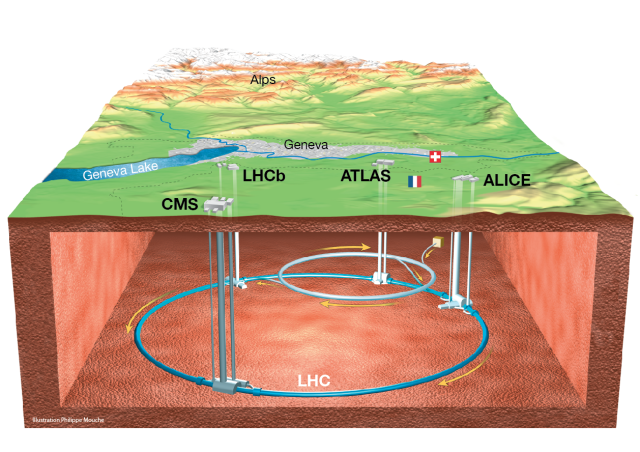
\includegraphics[width=0.70\textwidth]{Chapter02/LHC/Images/LHCUnderGroundDiagram.png}
  \caption{Underground diagram of the Geneva area showing the \gls{LHC} and its experiments location \cite{IMAGEREF:LHCDiagram}.}
  \label{FIGURE:ExperimentalApparatus_LHCLayoutUnderground}
\end{figure}

% Structure and experiments
The \gls{LHC} is a synchrotron machine with the capability of accelerating two particles beams in opposite directions in two separated beam pipes. These beams only cross and are forced to collide in four points of the accelerator where particle detectors are installed to observe the products of such collisions. This experiments are: \gls{ATLAS} \cite{ARTICLE:TheATLASExperiment}, \gls{CMS} \cite{ARTICLE:TheCMSExperiment}, \gls{LHCb} \cite{ARTICLE:TheLHCbExperiment} and \gls{ALICE} \cite{ARTICLE:TheALICEExperiment}.
% Add other experiments?

% Objective
The objective of the \gls{LHC} program is to investigate physics at the $\TeV$ scale, more specifically to understand the electroweak symmetry breaking and if this phenomena could be explained by the Higgs mechanism. There are many \gls{BSM} models that predict new physics at this energy regime making the \gls{LHC} the perfect machine to investigate such phenomena. \gls{ATLAS} and \gls{CMS} are general-purpose detectors which aim to investigate a broad spectrum of physics. The \gls{LHCb} detector is used to study processes that involve the decay of b-flavoured hadrons. The \gls{ALICE} detector is optimised to look at heavy-ion collisions and to investigate the properties of extreme high density medium that is formed.

% CERN accelerator chain
The \gls{LHC} is only the last element of a complex accelerator chain which step-by-step increases the energy of the particles to eventually be collided \cite{ARTICLE:LHCMachine}. Protons are initially obtained by stripping the electrons of hydrogen gas. This process happens at the begging of the \gls{LINAC2} which then accelerates them up to the energy of $50\,\MeV$. After this initial step proton are injected into the \gls{PSB} and the energy ramps ups to $1.4\,\GeV$. Particles are then passed to the \gls{PS} where the energy futher increases to $25\,\GeV$. Subsequently they are the injected into the \gls{SPS} where the particle energy level reaches $450\,\GeV$. Finally, protons pass to the \gls{LHC} where they can be accelerated to a maximum energy of $7\,\TeV$. A simplified diagram of the \gls{CERN} accelerator chain can be found in figure \ref{FIGURE:ExperimentalApparatus_LHCAccelaratorChain}. 
Normal operation of the \gls{LHC} therefore depends on all the upstream accelerators availability. The typically turn around time, the time necessary to stop the accelerator from running and restart collisions, is around 2 hours. When stable beams are achieved, a single proton fill can be used to collide protons up to 24 hours, but it is common to restart more frequently to profit from the higher collision rates possible right at the beginning of a new fill.

\begin{figure}[!htb]
  \centering
  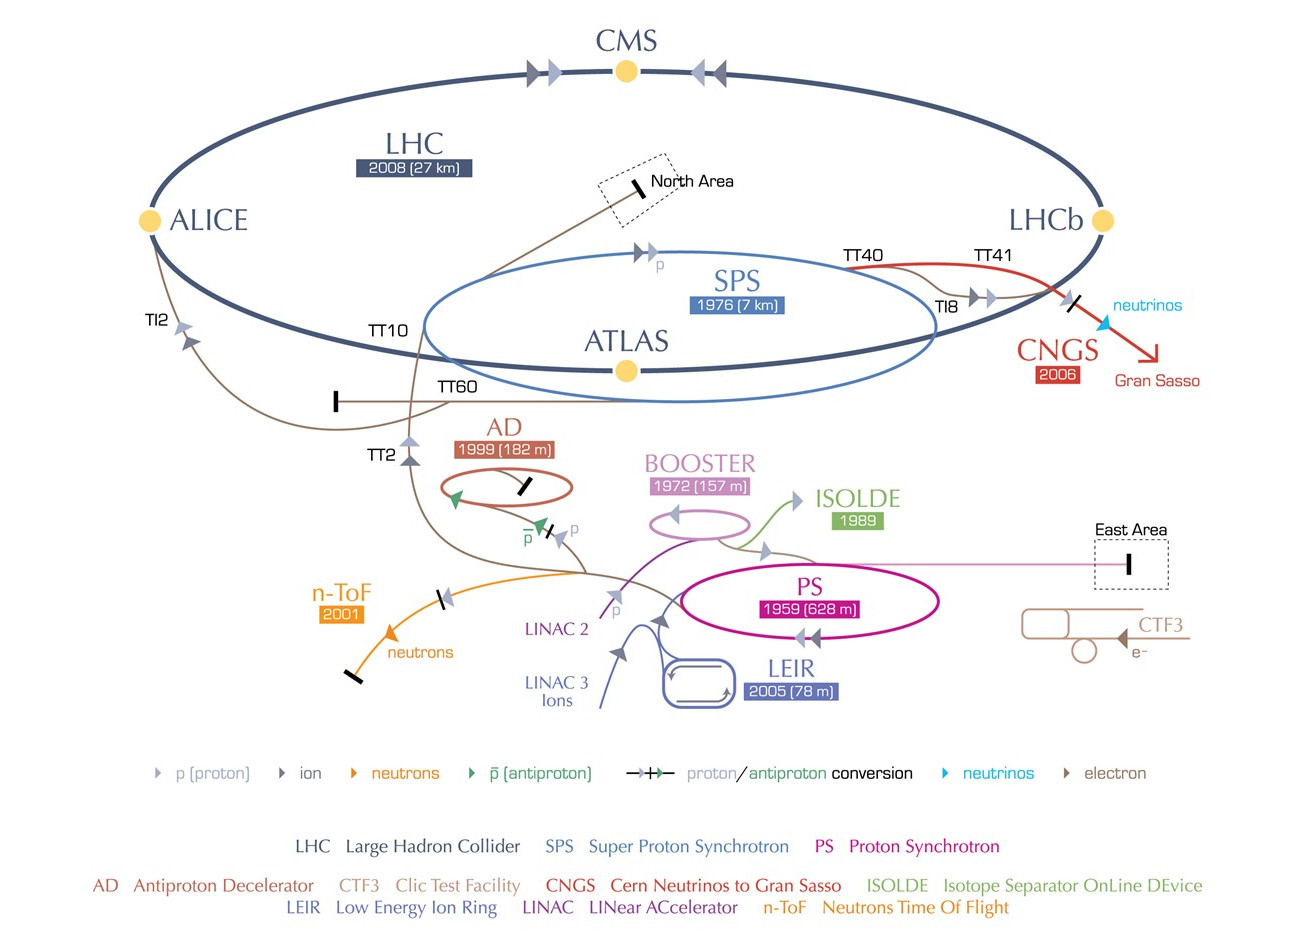
\includegraphics[width=0.90\textwidth]{Chapter02/LHC/Images/CERNAcceleratorComplex.jpg}
  \caption{Diagram of the \gls{CERN} accelerator complex \cite{IMAGEREF:CERNAcceleratorComplex}.}
  \label{FIGURE:ExperimentalApparatus_LHCAccelaratorChain}
\end{figure}

% LHC modes of opperation
Each beam pipe can be filled with proton or heavy ions. Three modes of operation have been tried: proton-proton, proton-lead ion and lead ion-lead ion. By changing the incoming particles we are changing the quantity of nucleons present at each interaction. The maximum design energy per proton is $7\,\TeV$ and is $2.76\,\TeV$ for each lead nucleon. The maximum design luminosity for proton-proton is $10^{34}\,\cm^{-2}\second^{-1}$ and $10^{27}\,\cm^{-2}\second^{-1}$ for lead ion-lead ion collisions.

% LHC structure
Particles beams trajectory are curved by 1232 niobium-titanium superconducting dipole magnets each with a length of $14.3\,\meter$. They are cooled with superfluid helium to $1.9\,\kelvin$ and produce the necessay magnetic field of $8.4\,\tesla$. Eight \gls{RF} cavities located at the \gls{LHC} point 4 are used to accelerate the beams. At each turn particle energy is increased to compensate for synchrotron radiation loss and increase the momentum. At nominal operation the \gls{LHC} will steer 2808 bunches composed up to $10^{11}$ protons separated by $25\,\ns$ in each direction. Some of the key parameters of the \gls{LHC} proton-proton and lead-lead operation can be found in table \ref{TABLE:ExperimentalApparatus_LHCMachineParameters}.

\begin{table}[!htb]
  \centering
  \begin{threeparttable}
    \begin{tabular}{|lcccc|}
    \hline 
                                  &              &           \textit{pp} &         \textbf{HI} &  \\
    \hline\hline
    Energy per nucleon            & E            &                     7 &                2.76 &                 $\TeV$ \\
    Dipole field at 7 TeV         & \textit{B}   &                  8.33 &                8.33 &               $\tesla$ \\
    Design Luminosity\tnote{*}    & $\mathcal{L}$ &            $10^{34}$ &           $10^{27}$ & $\cm^{-2}\second^{-1}$ \\
    Bunch separation              &              &                    25 &                 100 &                  $\ns$ \\
    No. of bunches                & $k_B$        &                  2808 &                 592 &                        \\
    No. particles per bunch       & $N_p$        & $1.15 \times 10^{11}$ & $7.0 \times 10^{7}$ &                        \\
    \hline
    \hline
    \textbf{Collisions}           &              &  &  &  \\
    \hline
    $\beta$-value at IP           & $\beta^{*}$  &                  0.55 &                 0.5 &        $\meter$ \\
    RMS beam radius at IP         & $\sigma^{*}$ &                  16.7 &                15.9 &  $\micro\meter$ \\
    Luminosity lifetime           & $\tau_L$     &                    15 &                   6 &         $\hour$ \\
    Number of collisions/crossing & $n_c$        &          $\approx 20$ &                   - &                 \\
    \hline
    \end{tabular}
    \begin{tablenotes}
      \item[*] For heavy-ion (HI) operation the design luminosity for Pb-Pb collisions is given.
    \end{tablenotes}
  \end{threeparttable}
  \caption[LHC parameters relevant for detectors]{The machine parameters relevant for the 
                                                  LHC detectors.\cite{CMSTDR:CMSPhysicsVol1}}
  \label{TABLE:ExperimentalApparatus_LHCMachineParameters}
\end{table}


At the \gls{LHC} we are looking for extremely rare processes. As is can be seen in figure \ref{FIGURE:ExperimentalApparatus_LHCCrossSections} the production cross section of a \gls{SM} Higgs boson is more than 9 orders of magnitude smaller than the total proton-proton cross section. 

\begin{figure}[!htb]
  \centering
  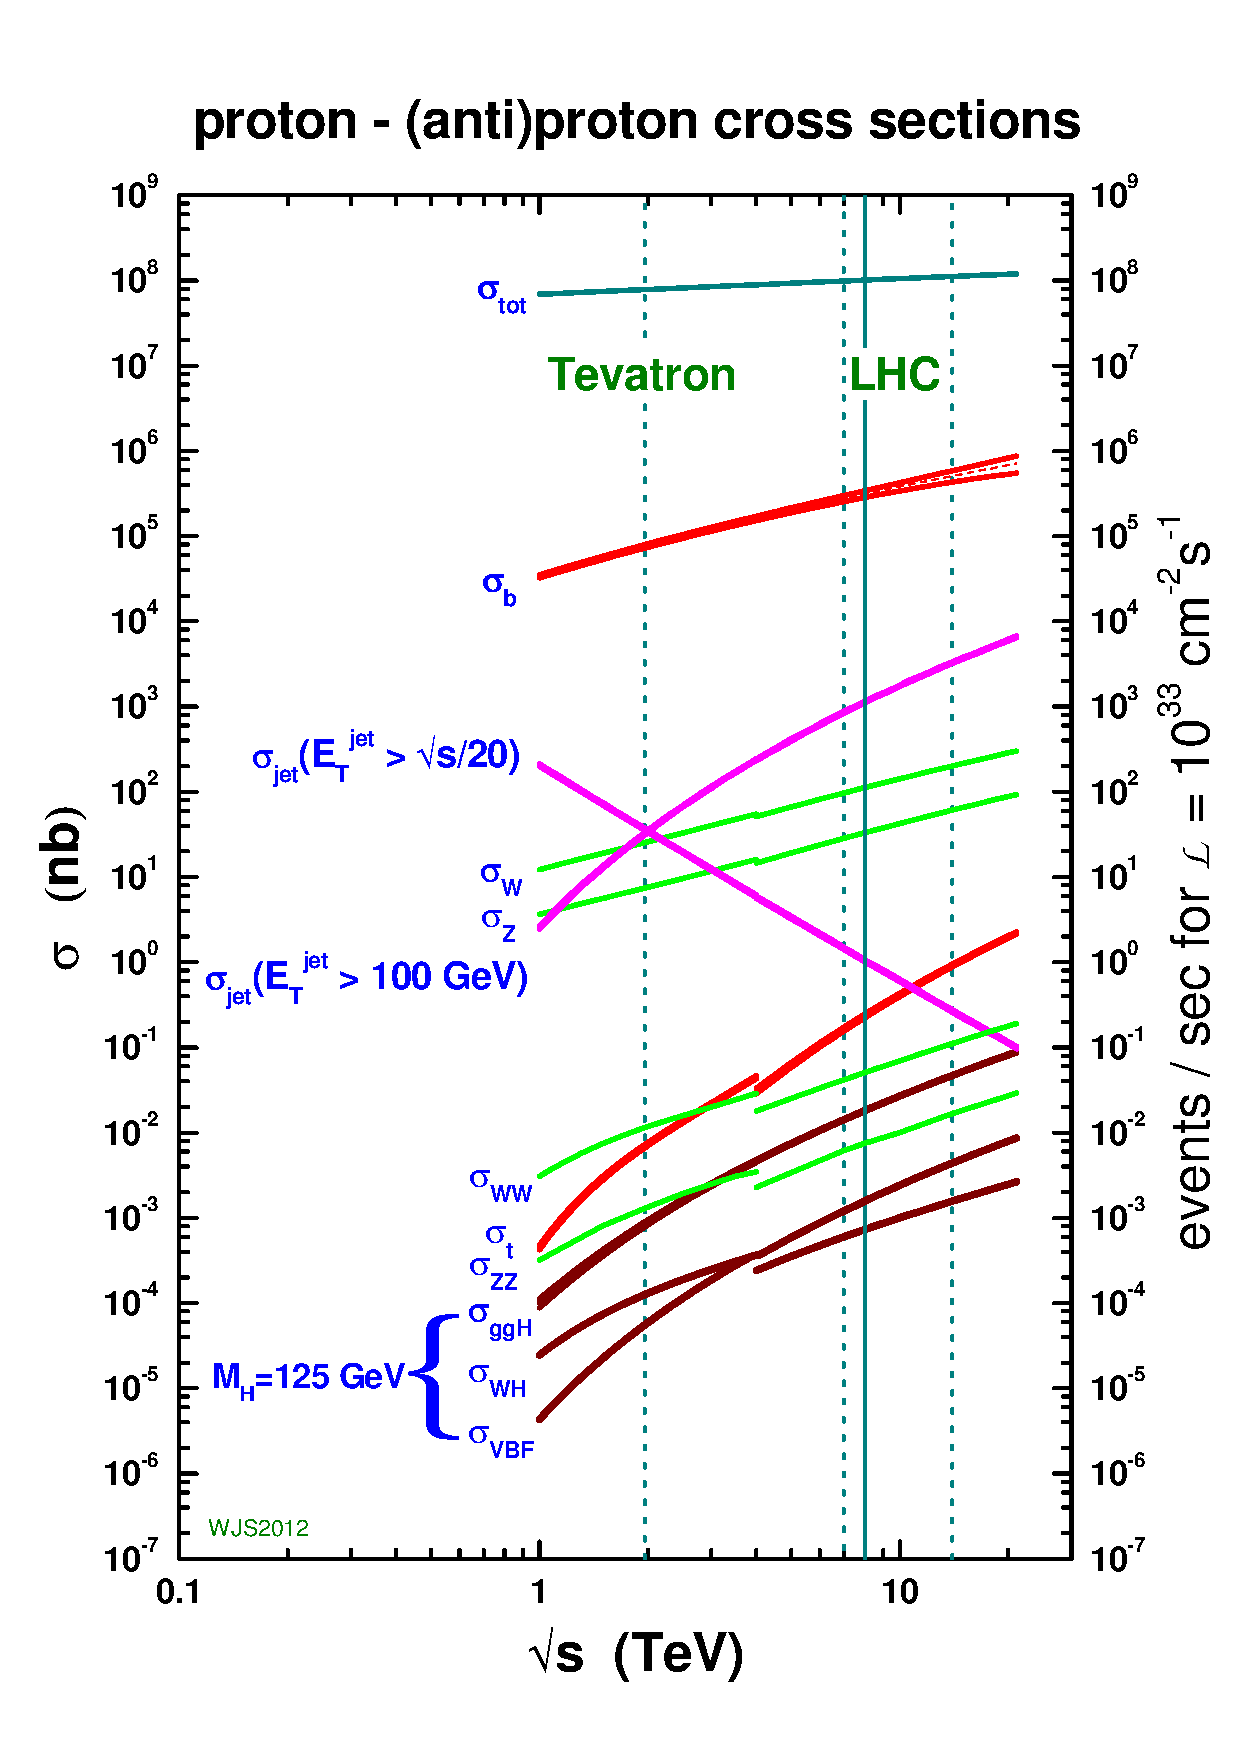
\includegraphics[width=0.50\textwidth]{Chapter02/LHC/Images/crosssections2012_v5}
  \caption{Cross sections for several processes for collisions of antiproton-proton and proton-proton as a function of the center of mass energy \cite{ARTICLE:TheCMSExperiment}.}
  \label{FIGURE:ExperimentalApparatus_LHCCrossSections}
\end{figure}

To be able to record and study such rare processes we need to produce a significant number of collisions. For this purpose the \gls{LHC} was designed to operate at high instantaneous luminosity, L. This quantity is defined as,

\begin{equation}
L=\frac{N_{b}^{2}n_{b}f_{\text{rev}}\gamma}{4\pi\epsilon_{n}\beta^{*}}F,
\end{equation}

where $N_{b}$ is the number of protons per bunch, $n_{b}$ is the number of bunches, $f_{\text{rev}}$ is the frequency of revolution, $\gamma$ is the Lorentz factor, $\epsilon_{n}$ is the normalized emittance, $\beta^{*}$ is the beta function at the collision point and $F$ is the reduction factor due to the crossing angle.

%%%%%%%%%%%%%%%%%%%%%%%%%%%%%%%%%%%%%%%%%%%%%%%%%%%%%%%%%%%%%%%%%%%%%%%%%%%%%%%%%%%%%%%
%%% SUBSECTION
%%%%%%%%%%%%%%%%%%%%%%%%%%%%%%%%%%%%%%%%%%%%%%%%%%%%%%%%%%%%%%%%%%%%%%%%%%%%%%%%%%%%%%%
\subsection{Running and performance}
\label{SUBSECTION:ExperimentalApparatus_CMS_RunningAndPerformance}

%Historical
Operation of the \gls{LHC} has started when the first beams circulated in the machine in September 2008. Unfortunately, only a few days after a faulty weld between two dipole magnets caused a significant magnet quench which in turn damaged several dipoles and a simultaneous leak of a significant amount of helium happened. The event showed that beyond the repair of the affected systems the accelerator needed a significant consolidation program to allow it to return to activity \cite{ARTICLE:CMSReportIncident19Sep2008}. This consolidation program took over one year to finalise and to prevent further possible problems and allow better understanding of the machine while maximizing physics reach, it was decided to initially run the \gls{LHC} at $7\,\TeV$ center-of-mass energy.
First collisions happened at November 2009 just at the \gls{SPS} injection energy of $450\,\GeV$ giving start to the \gls{LHC} run I.

The collision energy was finally ramped up to $7\,\TeV$ with first collisions being observed during March 2010. Operation at this energy continued until the end of 2011, with a peak luminosity being achieved of $3.7 \times 10^{33} \centi\meter^{-2}\second^{-1}$. The total integrated luminosity delivered to \gls{CMS} was $6.1\,\femto\barn^{-1}$ with the total actually recorded being $5.6\,\femto\barn^{-1}$. During 2012 with the increase knowledge of the accelerator it was possible to increase the centre-of-mass energy further to $8\,\TeV$ and eventually reaching peak luminosity of $7.7 \times 10^{33}\,\centi\meter^{-2}\second^{-2}$ and delivering integrated luminosity of $23.3\,\femto\barn^{-1}$ to \gls{CMS} of which $21.79,\femto\barn^{-1}$  $\femto\barn^{-1}$ were recorded. Figure \ref{FIGURE:ExperimentalApparatus_CMS_IntegratedLumi_pp_2010-2012} shows the delivered luminosity in the period 2010-2013 over time.

\begin{figure}[!htb]
  \centering
  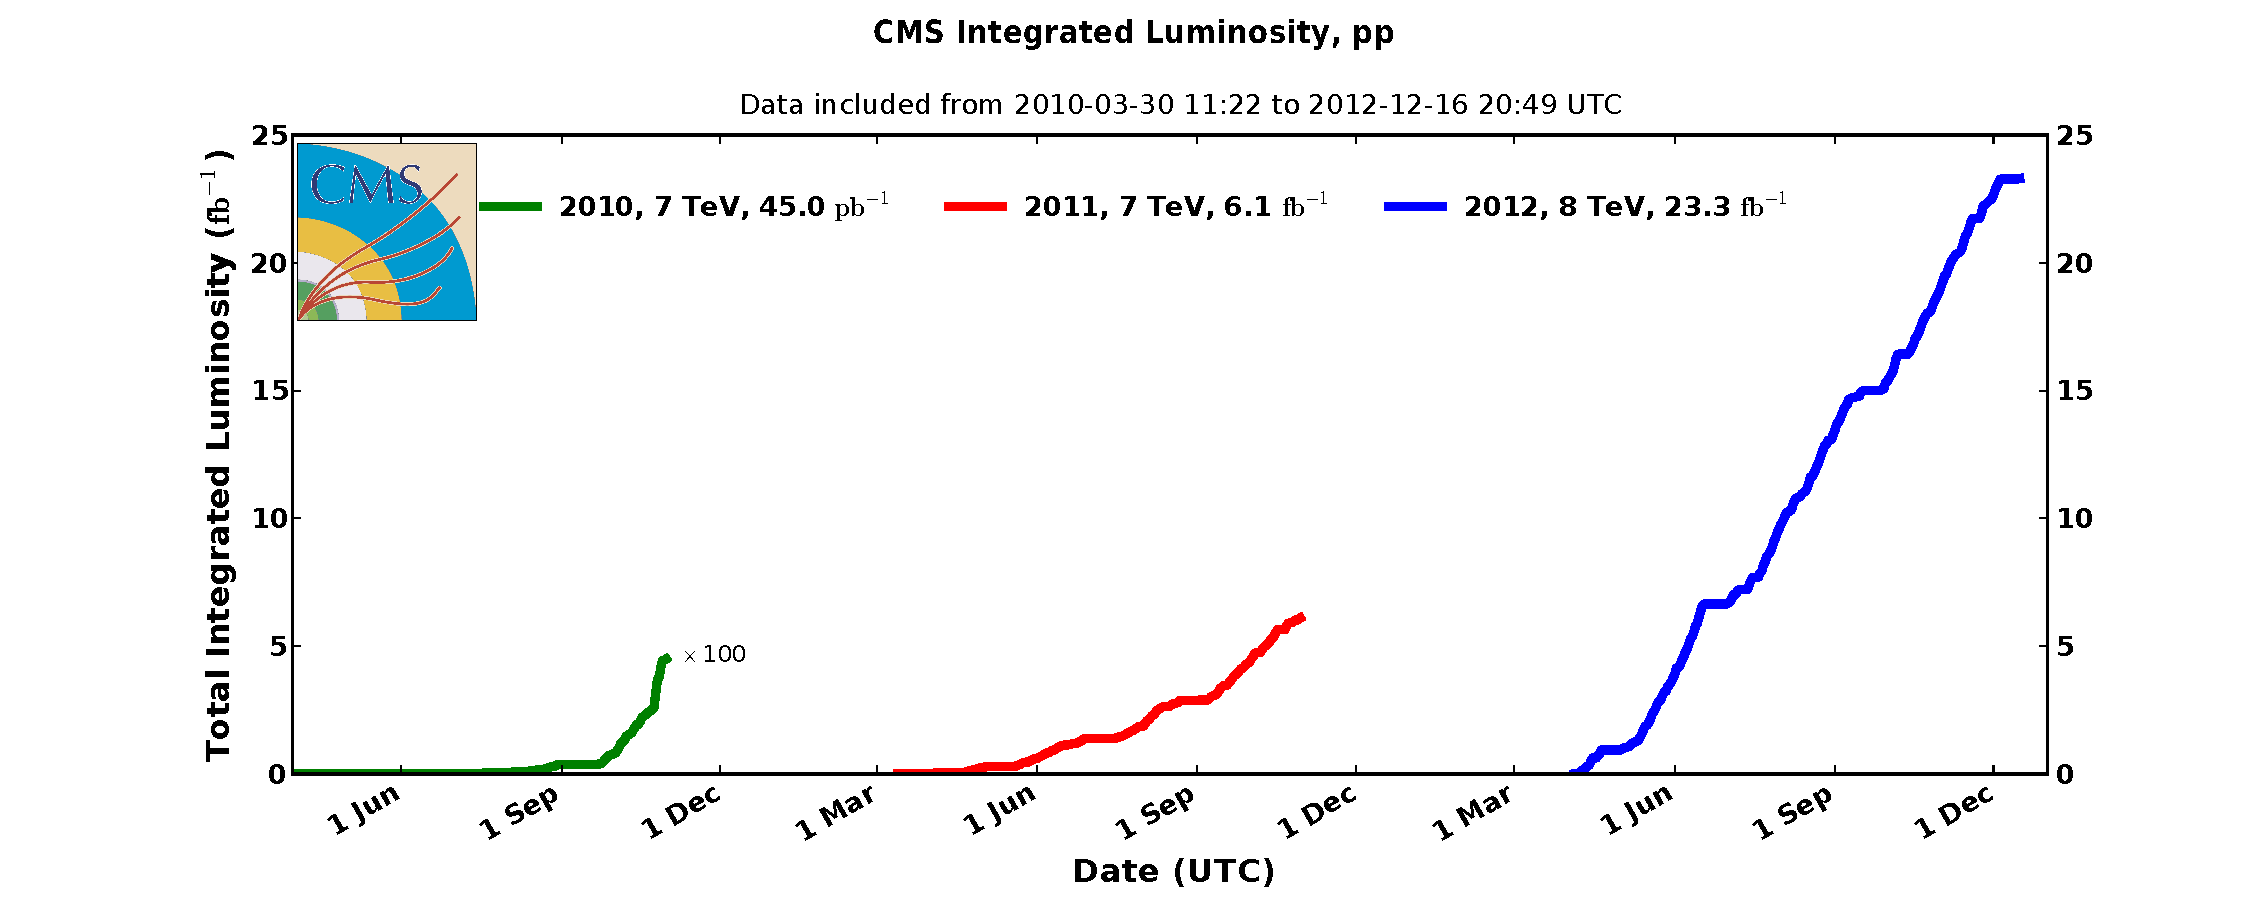
\includegraphics[width=1.00\textwidth]{Chapter02/CMS/Images/CMS_IntegratedLumi_pp_2010-2012}
  \caption{Cumulative luminosity versus day delivered to CMS during stable beams and for p-p collisions. This is shown for 2010 (green), 2011 (red) and 2012 (blue) data-taking \cite{IMAGEREF:CMSIntegratedLuminosity}.}
  \label{FIGURE:ExperimentalApparatus_CMS_IntegratedLumi_pp_2010-2012}
\end{figure}

For physics usage, data needs to undergo a certification process. In this process specialists from each \gls{CMS} subsystem check that no problem has happened during data taking that would bias or invalidate the recorded events. For 2011 a total of $5.1\,\femto\barn^{-1}$ and for 2012 a total $19.7\,\femto\barn^{-1}$ were considered of good quality for physics. 

In order to achieve high integrated luminosity \gls{LHC} collides particle bunches up to 40 million times a second, and many interactions may happen simultaneously, this effect is called \gls{PU}. Figure \ref{FIGURE:ExperimentalApparatus_CMS_PileIp_pp_2012} shows the distribution of the mean number of interaction per bunch crossing during 2012 at the \gls{CMS} experiment.

\begin{figure}[!htb]
  \centering
  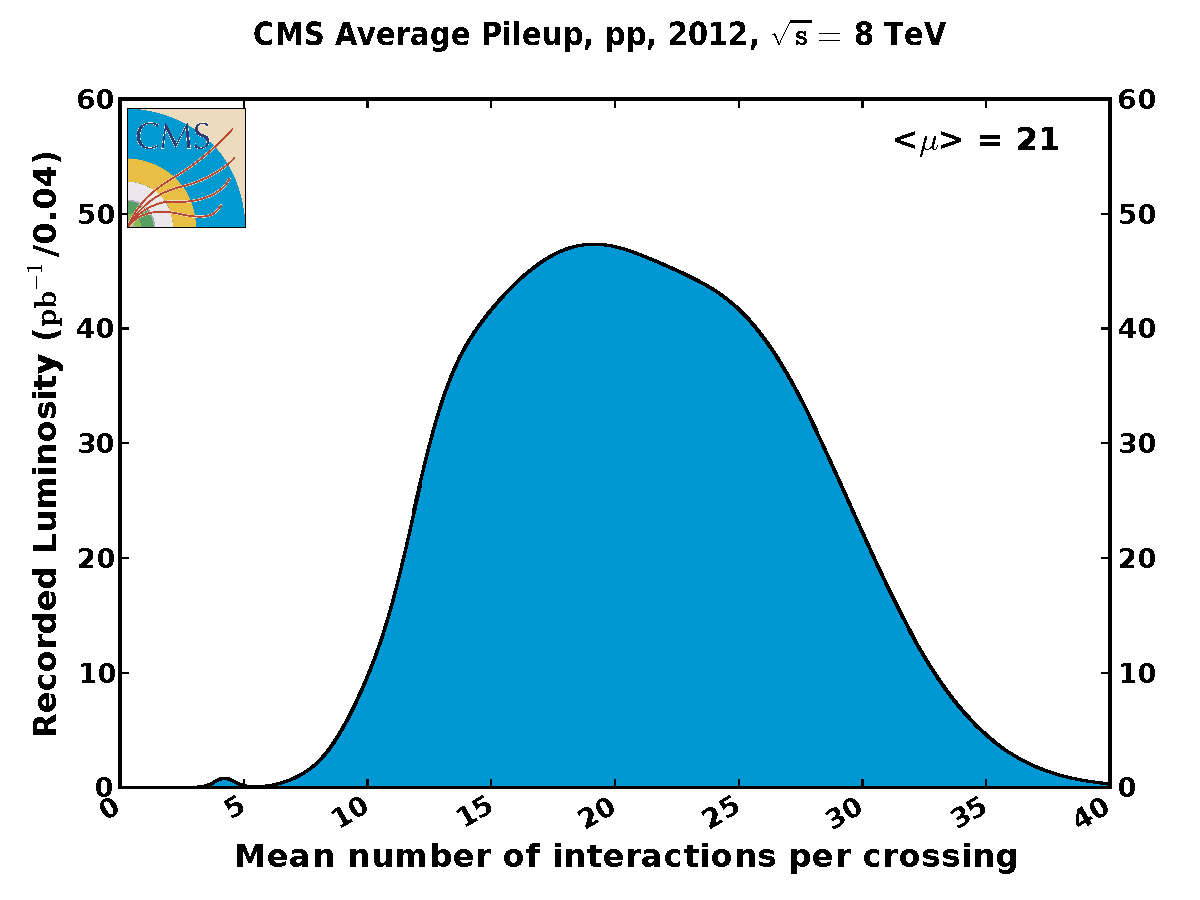
\includegraphics[width=0.60\textwidth]{Chapter02/CMS/Images/CMS_PileIp_pp_2012}
  \caption{Mean number of interactions per bunch crossing at the CMS experiment during 2012 \cite{IMAGEREF:CMSAveragePileUp2012}.}
  \label{FIGURE:ExperimentalApparatus_CMS_PileIp_pp_2012}
\end{figure}

%%%%%%%%%%%%%%%%%%%%%%%%%%%%%%%%%%%%%%%%%%%%%%%%%%%%%%%%%%%%%%%%%%%%%%%%%%%%%%%%%%%%%%%
%%% SECTION
%%%%%%%%%%%%%%%%%%%%%%%%%%%%%%%%%%%%%%%%%%%%%%%%%%%%%%%%%%%%%%%%%%%%%%%%%%%%%%%%%%%%%%%
\section{The Compact Muon Solenoid Experiment}
\label{SECTION:ExperimentalApparatus_CMS}

%Status: Done (needs review)

The \acrfull{CMS} experiment is a general purpose experiment located at the \gls{LHC} point 5, near the village of Cessy, France. It was designed to be a high performance detector studying collisions at its centre. It is composed of several subsystems in a classic onion shaped structure. A diagram of the experiment can be found in figure \ref{FIGURE:ExperimentalApparatus_CMS_Layout_Diagram}.

\begin{figure}[!htb]
  \centering
  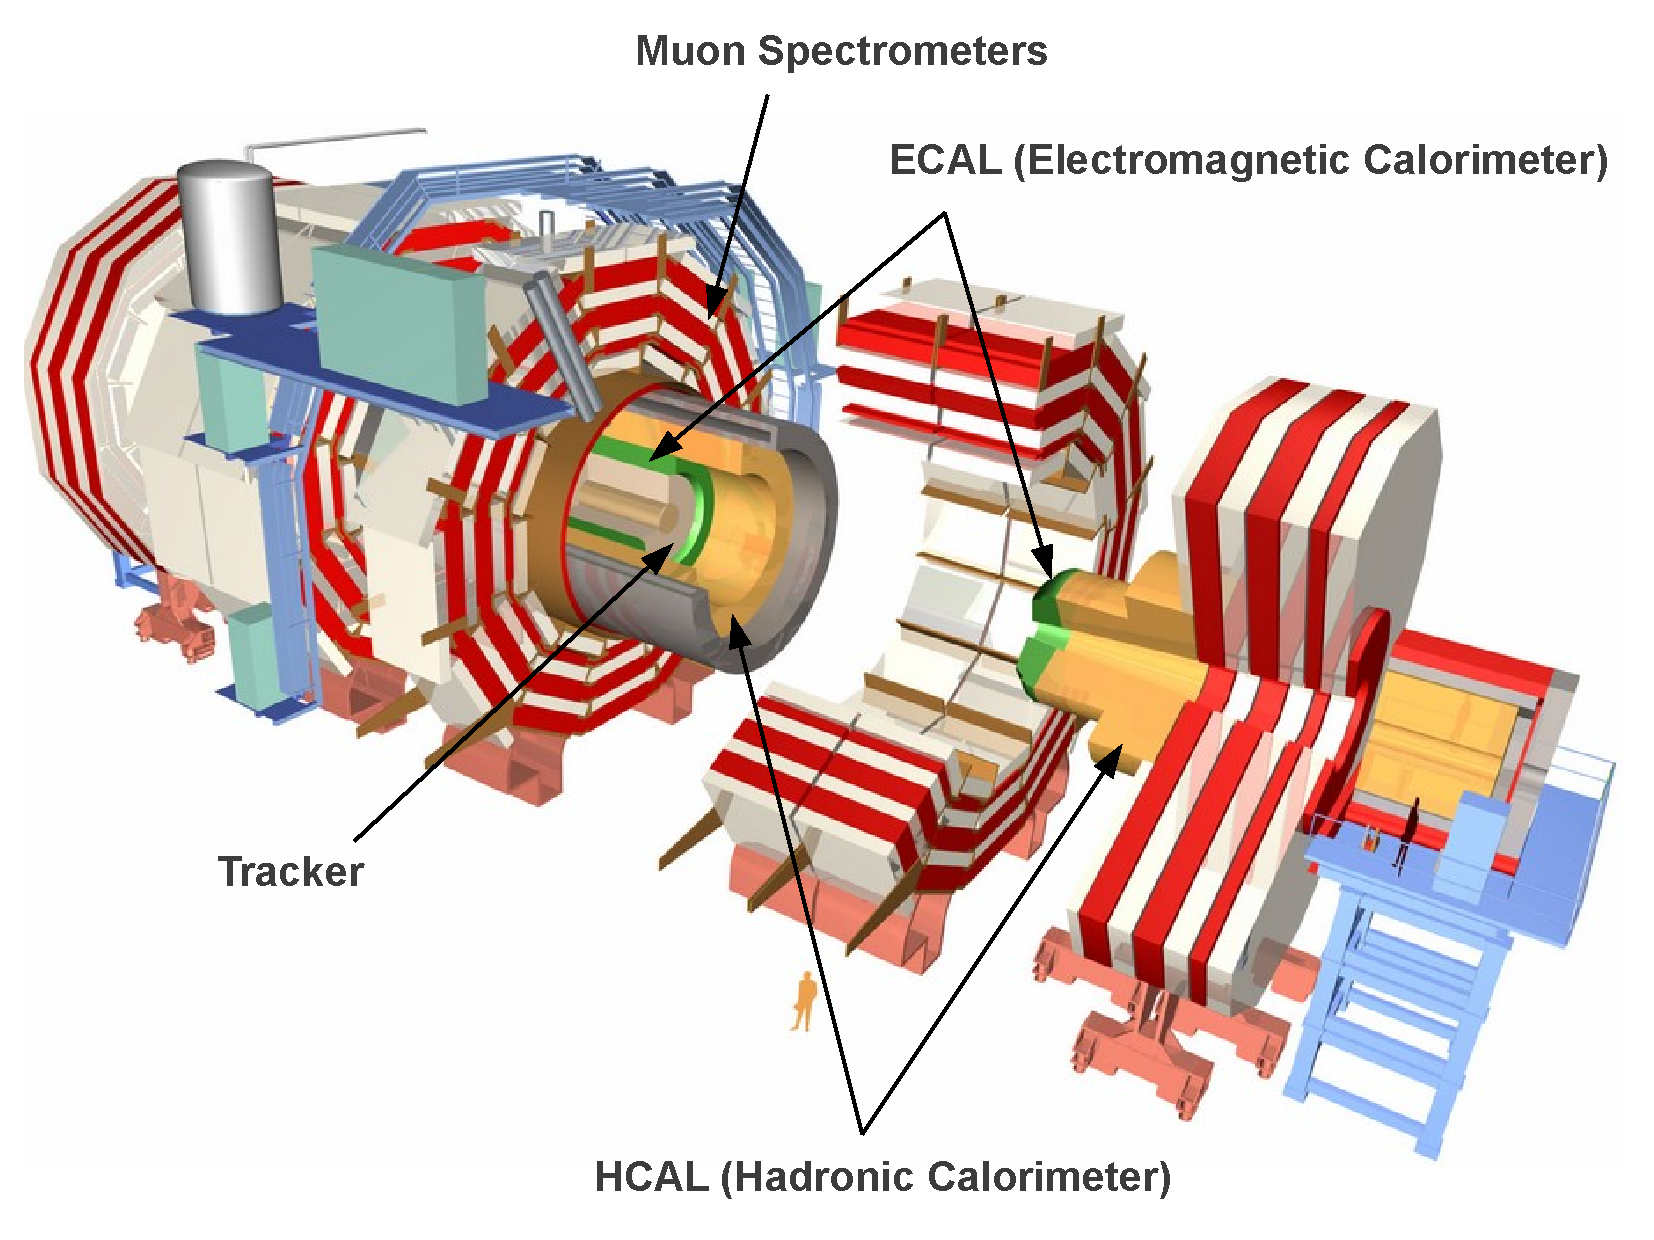
\includegraphics[width=1.00\textwidth]{Chapter02/CMS/Images/CMS_Layout_Diagram.pdf}
  \caption{Diagram of \gls{CMS} experiment showing the experiment in an open configuration and highlighting the position of its sub-detectors \cite{IMAGEREF:CERNPublic_CMSDiagram}.}
  \label{FIGURE:ExperimentalApparatus_CMS_Layout_Diagram}
\end{figure}

The main driving motivation for its design was to investigate the electroweak symmetry breaking and the Higgs mechanism at the design time was presumed to be the most likely explanation. Many alternative theories to the standard model predict new particles which could be observed at the $\TeV$ scale, \gls{CMS} as a multi-purpose experiment is well suited to search for these new scenarios. If found, such new physics may allow us to understand some of the currently open questions in particle physics, like providing a particle candidates for dark dark matter. Further more, some of these possible new physics signals could point the way towards a grand unified theory. \gls{CMS} is also capable of operating while the \gls{LHC} is colliding heavy ions and has a rich program covering the study of matter at extreme temperatures, densities and parton momentum fraction (low-x).

The requirements imposed on the \gls{CMS} design to meet its physics goals can be summarized in the following table \cite{ARTICLE:CMSTechnicalProposal,ARTICLE:TheCMSExperiment}:

\begin{itemize}
  \item Good muon identification and momentum resolution over a wide range of momenta and angles, good dimuon mass resolution ($\approx 1\%$ at $100\,GeV$), and the ability to determine un-ambiguously the charge of muons with $\pt<1\,\TeV$.
  \item Good charged-particle momentum resolution and reconstruction efficiency in the inner tracker. Efficient triggering and offline tagging of $\tau$'s and b-jets, requiring pixel detectors close to the interaction region.
  \item Good electromagnetic energy resolution, good diphoton and dielectron mass resolution ($\approx 1\%$ at $100\,\GeV$), wide geometric coverage, $\pi^0$ rejection, and efficient photon and lepton isolation at high luminosities.
  \item Good missing-transverse-energy and dijet-mass resolution, requiring hadron calorimeters with with a large hermetic geometric coverage and with fine lateral segmentation.
\end{itemize}

%TODO: Maybe re-write this!!!
The final detector design fulfils all these requirements. The experiment is compact compared to the other \gls{LHC} experiments being $22\,\meter$ long and $15\,\meter$ in diameter. Although small, it is the heaviest of the four big detectors at 12500 tonnes. Its high density is a direct consequence of it producing the highest magnetic field at $4\,\tesla$ and therefore needing more material for it to be contain in its return yoke. 

%%%%%%%%%%%%%%%%%%%%%%%%%%%%%%%%%%%%%%%%%%%%%%%%%%%%%%%%%%%%%%%%%%%%%%%%%%%%%%%%%%%%%%%
%%% SUBSECTION
%%%%%%%%%%%%%%%%%%%%%%%%%%%%%%%%%%%%%%%%%%%%%%%%%%%%%%%%%%%%%%%%%%%%%%%%%%%%%%%%%%%%
\subsection{Geometry and conventions}
\label{SECTION:ExperimentalApparatus_CMS_GeometryConventions}

% STATUS: DONE 

The adopted coordinate system has it origin in the center of \gls{CMS} where the nominal collision point is located, the \textit{y}-axis points vertically upwards, and the \textit{x}-axis points radially inward in the direction of the centre of the \gls{LHC}. The \text{z}-axis points along the beam line towards the Jura mountains from the \gls{LHC} point 5. The azimuthal angle $\phi$ is measured from the \textit{x}-axis in the \textit{x-y} plane. The polar angle $\theta$ is measured from the \textit{z}-axis.

We define pseudorapidity as $\eta = -ln(tan(\theta/2))$. All transverse quantities, like the transverse momentum ($p_\perp$), are measured in the transverse plane of beam axis. The imbalance of energy is also measured in the \textit{x-y} plane and is denoted as $E^{miss}_\perp$.

%%%%%%%%%%%%%%%%%%%%%%%%%%%%%%%%%%%%%%%%%%%%%%%%%%%%%%%%%%%%%%%%%%%%%%%%%%%%%%%%%%%%%%%
%%% SUBSECTION
%%%%%%%%%%%%%%%%%%%%%%%%%%%%%%%%%%%%%%%%%%%%%%%%%%%%%%%%%%%%%%%%%%%%%%%%%%%%%%%%%%%%
\subsection{Inner tracking system}
\label{SUBSECTION:ExperimentalApparatus_CMS_Tracker}

% STATUS: DONE (reviwed J.Pela x1)
%
% Writing points:
% * Closest detector to beam, measures trajectories of charged particles
% * With magnetic field measures momentum and charge of this particles
% * Allows vertexing (primary and secundary)
% * Different regions different occupancy
% * Final arranagement

The inner tracking system is the closest detector to the beam axis and the interaction region \cite{CMSTDR:CMSTracker,CMSTDR:CMSTrackerAddendum}. Its function is to measure the trajectory of all charged particles with momentum above 1 $\GeV$ being produced at each \gls{LHC} collision. With the help of the strong magnetic field produced by the \gls{CMS} magnet, particle trajectories are bent allowing for charge and momentum determination. With the resulting tracks is it then possible to determine the primary vertex as well as secondary vertexes like other lower energy proton-proton collision or displaced vertexes from the decay of long lived particles like B mesons.

Building a tracking system for an experiment at the \gls{LHC} is very challenging. Such system at design luminosity will be hit by an average of 1000 particles at a rate approaching $40\,\mega\hertz$. It needs to be a fast, efficient, high granularity detector, radiation hard and as thin as possible to not deflect the incoming particles trajectory. At each layer the occupancy should be of the order of $1\%$ or lower. This design requirements have lead to a tracker design entirely based on silicon detector technology. 

The volume near the interaction point can be split according to the charged particle flux into three regions:

\begin{itemize}
  \item $r<10\,\centi\meter$: highest particle flux, up to $\approx 10^8 \centi\meter^{-2}\second^{-1}$ at $r \approx 4 \centi\meter$, pixel detectors are used. The pixel size is $\approx 100 \times 150\,\micro\meter^2$, which translates into an occupancy of $10^{-4}$ per \gls{LHC} bunch crossing.
  \item $20<r<55\,\centi\meter$: particle flux decreases enough to use silicon micro-strips with a minimum cell size of $10\,\centi\meter \times 80\,\micro\meter$, leading to an occupancy of $\approx 2-3\%$ per \gls{LHC} bunch crossing.
  \item $50<r<110\,\centi\meter$: most outer region of the tracker, particle flux is low enough to use larger pitch silicon micro-strips. The maximum cell size is of $25\,\centi\meter$ $\times 180\,\micro\meter$, and occupancy is of the order of $\approx 1\%$.
\end{itemize}

The \gls{CMS} tracker final configuration is composed of a pixel detector with three barrel layers at radii between $4.4\,\centi\meter$ and $10.2\,\centi\meter$ and 2 disks on each side of the barrel. And a silicon strip tracker with 10 barrel detection layers extending up to $1.1\,\meter$ with 3 plus 9 disks on each side of the barrel. A schematic of this detector module distribution can be found at figure \ref{FIGURE:ExperimentalApparatus_CMS_Tracker_Layout}. This detector has an acceptance covering up to pseudorapidity of $|\eta|<2.5$ and has a total active area of about $200\,\meter^2$ making the largest silicon tracker ever built. 

\begin{figure}[!htb]
  \centering
  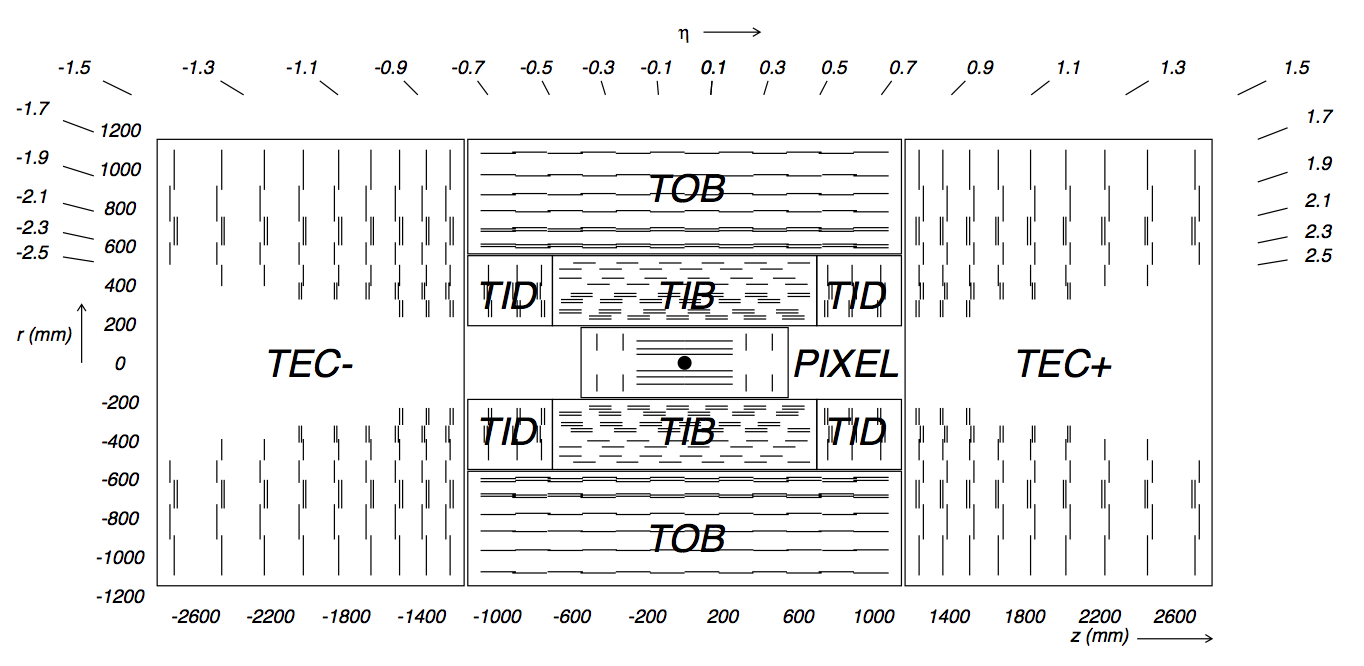
\includegraphics[width=1.0\textwidth]{Chapter02/CMS/Images/CMS_Tracker_Layout.png}
  \caption{Schematic cross section of the CMS tracker \cite{ARTICLE:TheCMSExperiment}. Each line represent a detector module. Double lines represent dual surface back-to-back detector modules. The inner tracker components are shown components: \gls{TEC}, \gls{TOB}, \gls{TID}, \gls{TIB} and Pixels. }
  \label{FIGURE:ExperimentalApparatus_CMS_Tracker_Layout}
\end{figure}

%%%%%%%%%%%%%%%%%%%%%%%%%%%%%%%%%%%%%%%%%%%%%%%%%%%%%%%%%%%%%%%%%%%%%%%%%%%%%%%%%%%%%%%
%%% SUBSECTION
%%%%%%%%%%%%%%%%%%%%%%%%%%%%%%%%%%%%%%%%%%%%%%%%%%%%%%%%%%%%%%%%%%%%%%%%%%%%%%%%%%%%
\subsection{Electromagnetic Calorimeter}
\label{SUBSECTION:ExperimentalApparatus_CMS_ECAL}

% Status: DONE (just with MSc input, and needs review)

The \gls{ECAL} is the detector responsible for measuring the energy of electrons and photons \cite{CMSTDR:CMSECAL,CMSTDR:CMSECALAddendum}. It is an hermetic energy measurement system comprised of 61200 lead tungstate ($PbWO_4$) crystals mounted in the barrel and 7324 crystals in each of the 2 endcaps and it has an acceptance up to $|\eta|<3.0$.

Lead tungstate has a fairly high density ($8.28\,\gram/\centi\meter^3$), has a short radiation length ($0.89\,\centi\meter$) and a small Moliere redius ($2.2\,\centi\meter$). The crystals also have a fast scintillation decay time emitting 80\% of the light yield in $25\,\nano\second$ (the minimal bunch crossing time at the \gls{LHC}). This characteristics make it a good choice for an electromagnetic calorimeter allowing a compact design with fine granularity. However, this crystals emit a fairly low light yield ($30\,\gamma/\MeV$) which requires the use of photo-detectors with intrinsic gain which will preform well inside a magnitic field. In the barrel region silicon \gls{APD} are used and \gls{VPT} are used in the endcaps. To guarantee good response from both crystals and \gls{APD} it is necessary to have system thermal stability, with the goal being temperature variation of less than $0.1 \celsius$.

The barrel section, the \gls{EB}, has an inner radius of $129\,\centi\meter$ and is composed of 36 identical ``supermodules'', each covers the barrel length and corresponding to a pseudo-rapidity interval of $0<|\eta|<1.479$. The crystals are quasi-projective (the axes are tilted at 3º with respect to the line from the nominal vertex position) and cover 0.0174 (i.e. 1º ) in $\Delta\phi$ and $\Delta\eta$. The crystals have a front face cross-section of $\approx 22 \times 22\,\milli\meter^2$ and a length of $230\,\milli\meter$, corresponding to 25.8 $X_0$.

The endcap section, the \gls{EE}, is at a distance of $314\,\centi\meter$ from the vertex and covering a pseudorapidity range of $1.479<|\eta|<3.0$, are each structured as 2 ``Dees'', consisting of semi-circular aluminium plates from which are cantilevered structural units of $5\times 5$ crystals, known as ``supercrystals``. A diagram of the \gls{ECAL} can be found on figure \ref{FIGURE:ExperimentalApparatus_CMS_ECAL_Layout}.

\begin{figure}[!htb]
  \centering
  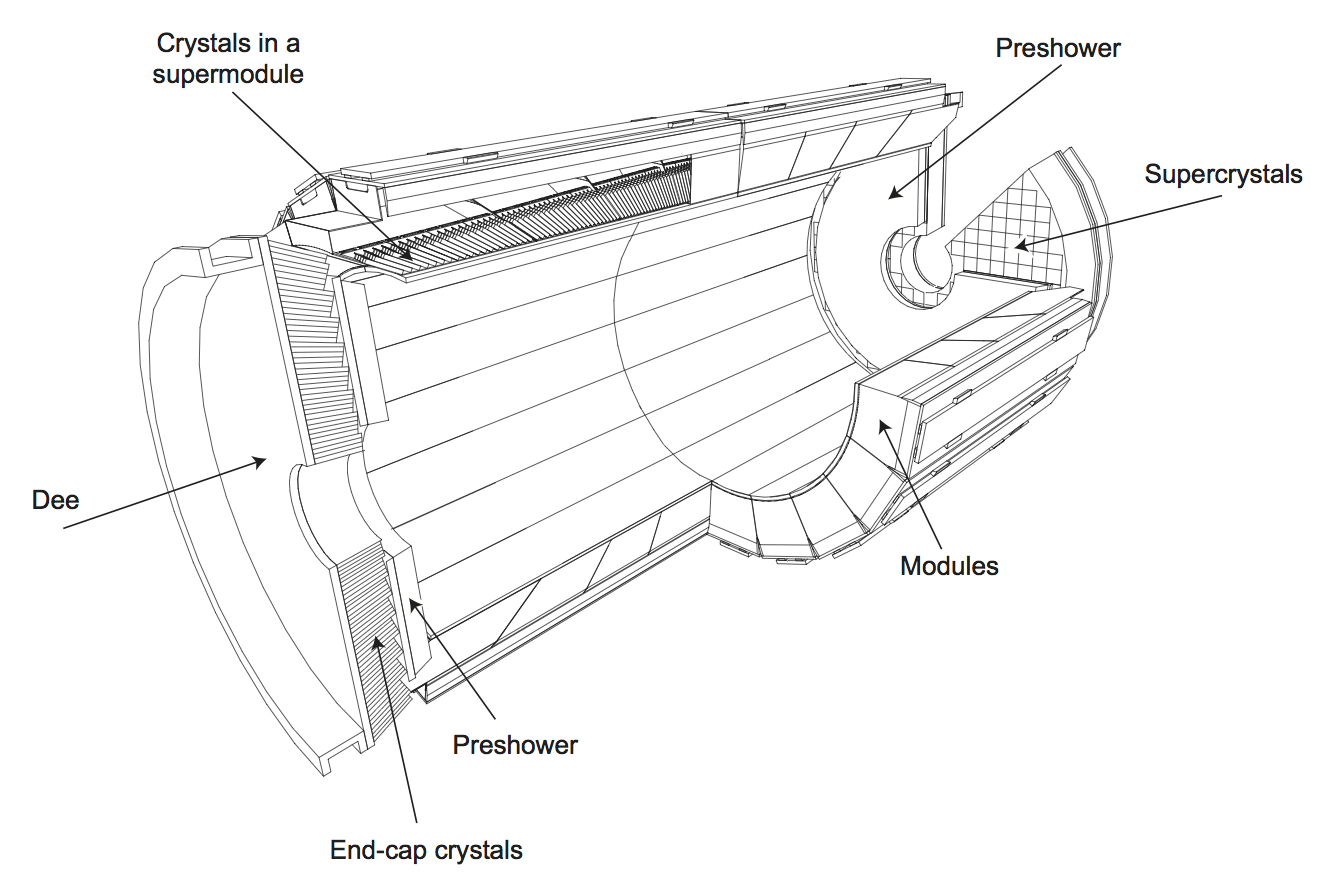
\includegraphics[width=0.8\textwidth]{Chapter02/CMS/Images/CMS_ECAL_Layout.png}
  \caption{Diagram of the ECAL layout illustrating the positions of its components \cite{ARTICLE:TheCMSExperiment}.}
  \label{FIGURE:ExperimentalApparatus_CMS_ECAL_Layout}
\end{figure}
 
The energy resolution of the \gls{ECAL} can be can be expressed as: 

\begin{equation}
\frac{\sigma}{E} = \frac{S}{\sqrt{E}} \oplus \frac{N}{E} \oplus C
\end{equation}

Here $E$ is the energy of the incoming particle, $S$ is the stochastic term which quantifies the fluctuations in scintillation and lateral containment of the shower, $N$ the noise term which relates with electronics and digitisation process and finally $C$ is a constant term that quantifies the non-uniform longitudinal response and inter-calibration errors. These parameters have been measured to be  $S=0.028\,\GeV^{1/2}$, $N=0.12\,\GeV$ and $C=0.003$ with the help of an electron beam \cite{ARTICLE:CMSECALTestBeam} and in the absence of magnetic field.

%%%%%%%%%%%%%%%%%%%%%%%%%%%%%%%%%%%%%%%%%%%%%%%%%%%%%%%%%%%%%%%%%%%%%%%%%%%%%%%%%%%%%%%
%%% SUBSUBSECTION
%%%%%%%%%%%%%%%%%%%%%%%%%%%%%%%%%%%%%%%%%%%%%%%%%%%%%%%%%%%%%%%%%%%%%%%%%%%%%%%%%%%%
\subsubsection{Preshower detector}
\label{SUBSUBSECTION:ExperimentalApparatus_CMS_ECAL_Preshower}

The \gls{CMS} Preshower is a detector locate in each endcap covering the fiducial region of $1.653<|\eta|<2.6$. Its mission is to identify neutral pions decay, help to identify electrons against minimum ionizing particles and improve electron and photon position determination.

This detector is sampling calorimeter composed by two layers of lead radiators each followed by silicon strip sensors. The lead layers have the function of forcing the incoming particles to initiate an electromagnetic shower. The first lead layer had $2X_0$ while the secong had $1X_0$, which results in 95\% of the single incident photons starting their shower before hitting the first sensor \cite{ARTICLE:TheCMSExperiment}. The shape of the lead layers edge matches the \gls{ECAL} crystal behind them to facilitate calculations at the \gls{L1T}.

Each silicon sensors have an active area of $61 \times 61\,\milli\meter$ and are $320\,\micro\meter$ thick. The sensors are divided into 32 strips each with $1.9\,\milli\meter$.  The preshower system has a total thickness of $20\,\centi\meter$ and had 137000 individual read-out channels. 

%%%%%%%%%%%%%%%%%%%%%%%%%%%%%%%%%%%%%%%%%%%%%%%%%%%%%%%%%%%%%%%%%%%%%%%%%%%%%%%%%%%%%%%
%%% SUBSECTION
%%%%%%%%%%%%%%%%%%%%%%%%%%%%%%%%%%%%%%%%%%%%%%%%%%%%%%%%%%%%%%%%%%%%%%%%%%%%%%%%%%%%
\subsection{Hadronic Calorimeter}
\label{SUBSECTION:ExperimentalApparatus_CMS_HCAL}

% STATUS: DONE

The \acrfull{HCAL} is a sampling calorimeter which is designed to measure the properties of hadron jets and indirectly neutrinos or other undiscovered particles that would result in apparent missing energy \cite{CMSTDR:CMSHCAL}. The design of the \gls{HCAL} was strongly influenced by the choice of the magnet parameters since most of the calorimetry is inside of the magnet. A diagram of the \gls{HCAL} subsystems and their location inside \gls{CMS} can be found in figure \ref{FIGURE:ExperimentalApparatus_CMS_HCAL_Layout}.

\begin{figure}[!htb]
  \centering
  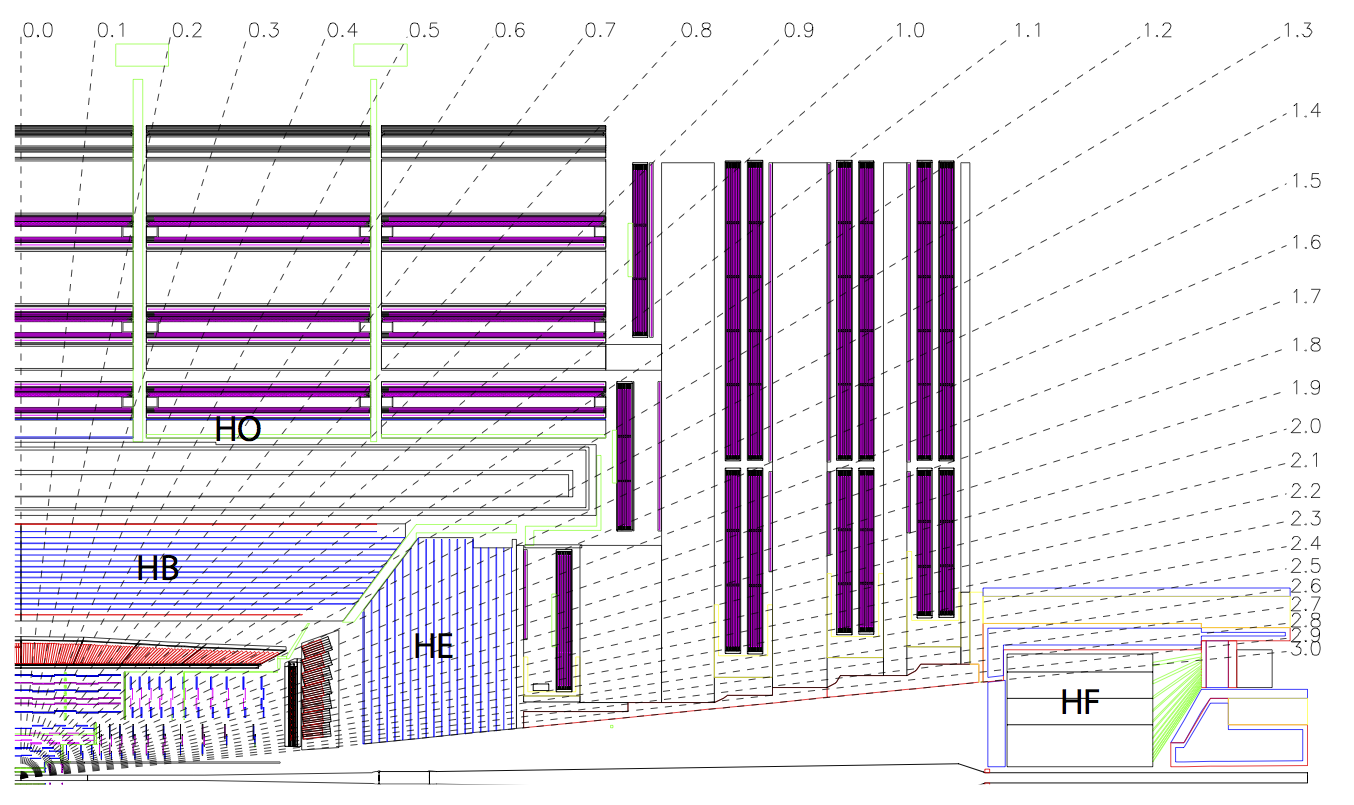
\includegraphics[width=1.0\textwidth]{Chapter02/CMS/Images/CMS_HCAL_Layout.png}
  \caption{Longitudinal view of the CMS detector highlighting the location of the \gls{HCAL} components: \gls{HB}, \gls{HE} \gls{HO} and \gls{HF} \cite{ARTICLE:TheCMSExperiment}.}
  \label{FIGURE:ExperimentalApparatus_CMS_HCAL_Layout}
\end{figure}

The \acrfull{HB} covers the region up to $|\eta|<1.3$ and is limited from the beam side by the \gls{ECAL} at radius $r=1.77\,\meter$ and outwards by the magnet at radius $r=2.95\,\meter$. This is a strict limitation on the amount of absorber material to be used. This detector is composed of 36 identical azimuthal wedges split in two half-barrels. They are constructed of brass absorber plates alternated with plastic scintillator. Brass has a short interaction length ($X_0=16.42\,\centi\meter$) and is non-magnetic. The detector is composed of 2304 towers with a segmentation of $\Delta\eta \times \Delta\phi = 0.087 \times 0.087$ which corresponds to the same area of a $5 \times 5$ arrays of \gls{ECAL} crystals.

To improve the measurement capability, an outer calorimeter, the \acrfull{HO}, is placed outside of the magnet as a \textit{tail catcher}. It increases the effective thickness of the hadronic calorimeter by over 10 interaction lengths. This detector covers the range $|\eta|<1.26$, it is composed or iron absorber and scintillator and is subdivided into sectors that cover 30º azimuthal angle in each of the barrel wheels. 

The \acrfull{HE} covers the range of $1.3<|\eta|<3.0$. It is composed by 2034 towers with a 14 towers segmentation in $\eta$ and 5º segmentation in $\phi$. The 8 inner most towers the segmentation is 10º in $\phi$, whilst the $\eta$ segmentation increases in $\eta$ from 0.09 to 0.35.

Additionally, to extend acceptance to $|\eta|<5.2$ the \gls{HF} is installed at $11.2\,\meter$ from the interaction point providing excellent hermeticity for $E_{\perp}^{miss}$ measurement. Its steel absorber is $1.65\,\meter$ deep and has quartz fibres running through it, parallel to the beam line. The energy measurement is made via Cerenkov light produced by the incoming particles inside the fibres. There are 13 tower in $\eta$ with segmentation of $\approx \Delta\eta=0.175$ except the lowest $\eta$ tower with $\approx \Delta\eta=0.1$ and highest $\eta$ tower with $\approx \Delta\eta=0.3$. The segmentation in $\phi$ is of $\Delta\phi=10º$ except in the highest $\eta$ towers which is $\Delta\phi=20º$. There are a total of tower 900 per \gls{HF} module. 

Similarly to the \gls{ECAL} the energy resolution \gls{HCAL} was tested using a test beam of single charged pions \cite{ARTICLE:CMSECALTestBeam}, and it was obtained that:

\begin{equation}
\frac{\sigma}{E} = \frac{94.3\%}{\sqrt{E}} \oplus 8.4\%.
\end{equation}

%%%%%%%%%%%%%%%%%%%%%%%%%%%%%%%%%%%%%%%%%%%%%%%%%%%%%%%%%%%%%%%%%%%%%%%%%%%%%%%%%%%%
%%% SUBSECTION
%%%%%%%%%%%%%%%%%%%%%%%%%%%%%%%%%%%%%%%%%%%%%%%%%%%%%%%%%%%%%%%%%%%%%%%%%%%%%%%%%%%%
\subsection{Solenoid Magnet}
\label{SUBSECTION:ExperimentalApparatus_CMS_Magnet}

%Status: DONE

The design requirements for correct charge assignment and \pt determination for charge particles and specially muons drive the magnet parameters choice. For muons, unambiguously charge determination requires momentum resolution of $\Delta p/p \approx 10\%$ at $p = 1 \TeV$. This requirements are specially difficult to obtain in the forward regions but with the correct length/radius ratio can be obtained with a modestly sized solenoid magnet but with large field \cite{CMSTDR:CMSPhysicsVol1,CMSTDR:CMSMagnet}.

The choice of the \gls{CMS} collaboration was to build a Niobium-Titanium (NbTi) superconducting solenoid magnet which has been design to operate at fields up to $4\,\tesla$ it has a diameter of $6\,\meter$ and a length of $12.5\,\meter$ at maximum field the stored energy reaches $2.7\,\giga\joule$. Typically, the magnet is only run at $3.8\,\tesla$ in order to maximize its lifetime. To contain such an enormous magnetic flux a $10\,\kilo\ton$ return yoke envelopes the magnet with 5 wheels in the barrel region and 2 endcaps composed of 3 disks closing the sides \cite{ARTICLE:TheCMSExperiment}. A summary of the most important magnet parameters can be found at table \ref{TABLE:ExperimentalApparatus_CMSMagnetParameters}.

\begin{table}[!htb]
  \centering
  \begin{tabular}{|l|c|}
  \hline
  Parameter & Value \\
  \hline\hline
  Field           & 4 T \\
  Inner Bore      & 5.9 m \\
  Length          & 12.9 m \\
  Number of turns & 2168 \\
  Current         & 19.5 kA \\
  Stored Energy   & 2.7 GJ \\
  Hoop Stress     & 64 atm \\
  \hline
  \end{tabular}
  \caption[Parameters of the CMS superconducting solenoid]{Parameters of the CMS superconducting solenoid}
  \label{TABLE:ExperimentalApparatus_CMSMagnetParameters}
\end{table}


%%%%%%%%%%%%%%%%%%%%%%%%%%%%%%%%%%%%%%%%%%%%%%%%%%%%%%%%%%%%%%%%%%%%%%%%%%%%%%%%%%%%
%%% SUBSECTION
%%%%%%%%%%%%%%%%%%%%%%%%%%%%%%%%%%%%%%%%%%%%%%%%%%%%%%%%%%%%%%%%%%%%%%%%%%%%%%%%%%%%
\subsection{Muon System}
\label{SUBSECTION:ExperimentalApparatus_CMS_Moun}

%Status: DONE (needs review)

The muon detection is an important part of the mission of \gls{CMS} \cite{CMSTDR:CMSMuonSystem}. Muons are fairly easy to detect when compared with other elementary particles and are only rarely produced in proton-proton collisions. To take the example of the \gls{SM} Higgs boson, while the decay mode involving a pair of Z bosons is fairly unlikely compared with other decays the Z bosons can decay into 4 mouns. This decay while rare does not have significant backgrounds making it a ''golden channel`` for discovery, which indeed was proven the case \cite{ARTICLE:CMSHiggsObservation}. Many other models, like SUSY, use muon final states in their searches exactly for the same reason. The \gls{CMS} muon system is composed of 3 types of gaseous detectors depending on they location and momentum reconstruction needs. A diagram of the disposition of this system inside \gls{CMS} can be found on figure \ref{FIGURE:ExperimentalApparatus_CMS_Muon_Layout}.

\begin{figure}[!htb]
  \centering
  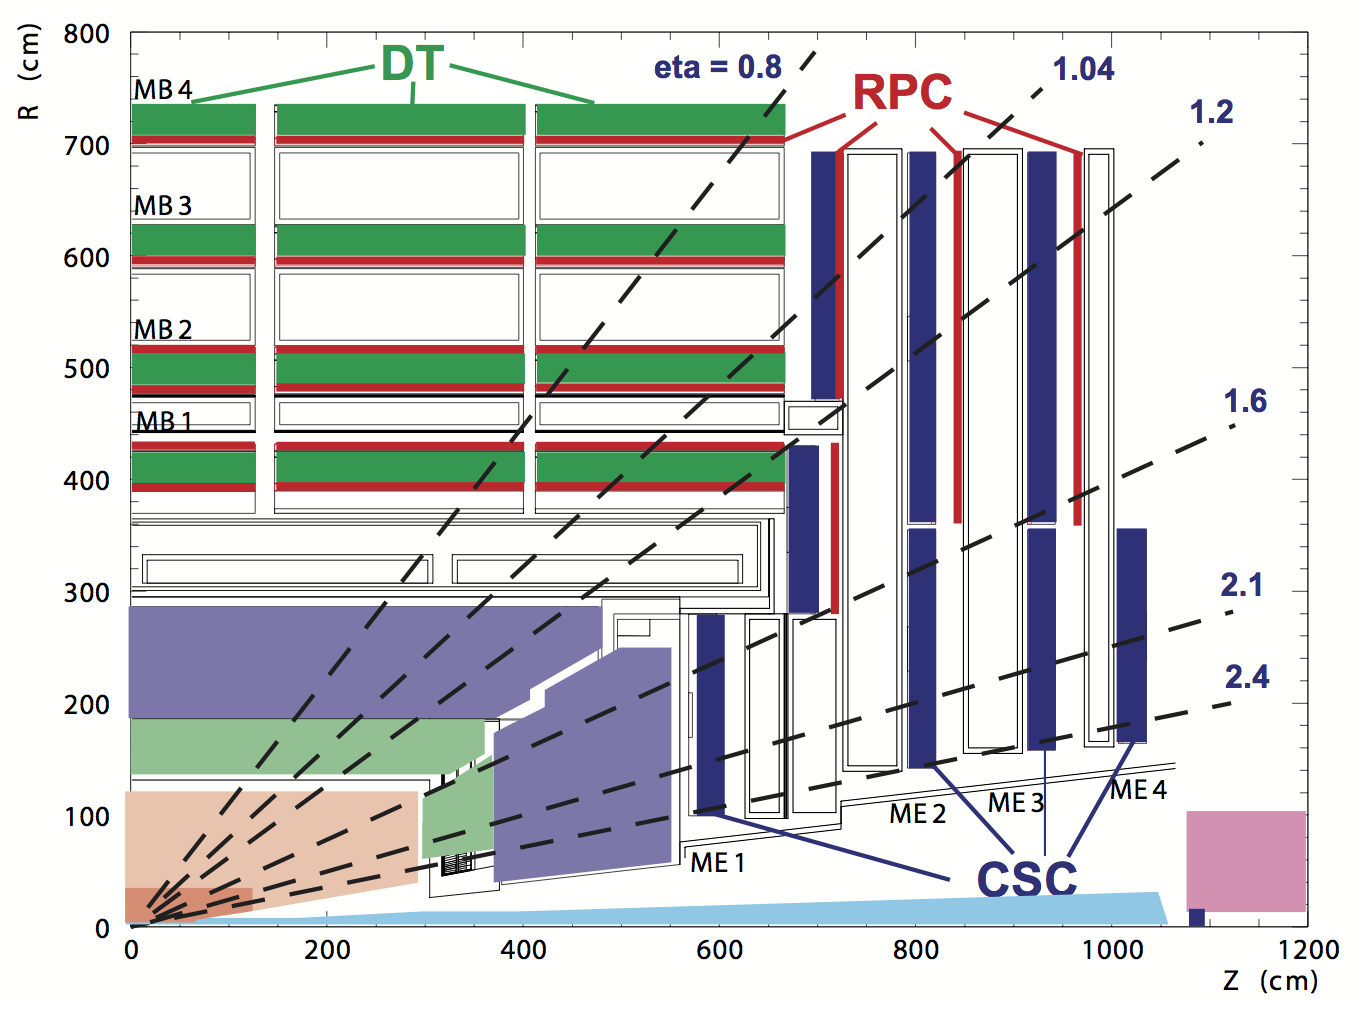
\includegraphics{Chapter02/CMS/Images/CMS_Muon_Layout.png}
  \caption{Diagram of the \gls{CMS} muon systems. The location of each muon chamber for each subsystem is showed \cite{CMSTDR:CMSPhysicsVol1}.}
  \label{FIGURE:ExperimentalApparatus_CMS_Muon_Layout}
\end{figure}

In the barrel and up to $|\eta|<1.2$, \gls{DT} are used. since the neutron background is small and the field is constant. This system is composed 250 chambers and is arranged in 4 concentric cylindrical layers which are installed inside of the return yoke. This chambers have a total of 172000 wires with a length of $2.4\,\meter$ which are housed inside of tubes filled with a mixture of argon and carbon-dioxide. Each of the wheels of the barrel is split into 12 sectors covering 30º azimuthal angle. The maximum gas ionization drift is of $2.0\,\centi\meter$ and results in a single point resolution is $\approx 200\,\micro\meter$ per wire. For each station each measured muon the $\phi$ resolution is better than $200\,\micro\meter$ and direction resolution is $\approx 1\,\milli\radian$.

In the endcaps \gls{CSC} are used in the region between $2.4>|\eta|>0.9$. Here, muon and background rates are high and the magnetic field is not uniform. This system has fast response and is radiation resistant. It is composed by 468 chambers arranged in 4 stations per side. Each chamber is trapezoidal in shape and made of 6 gas gaps and covers either 10º or 20º in $\phi$. Each gap contains a plane of cathode strips and a plane of anode wires. For each chamber the spacial resolution is of the order of $200\,\micro\meter$ and the angular resolution is $\approx 10\,\milli\radian$ in $\phi$.

Finally the \gls{RPC} covers the $|\eta|<1.6$ range. This system overlaps with the 2 other muon systems. It is very fast with an ionization event being much faster than the bunch crossing time. This fast response allows, in conjunction with a dedicated trigger system, to select the correct bunch crossing associated with the detection of a muon. In the barrel there 480 rectangular chambers arranged in 4 stations with 6 \gls{RPC} layers (2 layers are present in the 2 stations closest to the beam pipe). In the endcaps there are 3 \gls{RPC} disk shaped stations on each side, which are composed by trapezoidal shaped detectors.

The combined muon system offline momentum resolution is of the order of 9\% for small values of $\eta$ and $p$ and for transverse momenta of up to $200\,\GeV$. At higher energies of around $1\,\TeV$ the standalone momentum resolution is in the range of 15-40\% depending on $|\eta|$. This values are limited by the muon multiple-scattering before arriving to the muon system. If we combine the tracker information into a global fit the resolution for lower \pt tracks improves an order of magnitude while at higher momenta (around $1\,\TeV$) it is of about 5\%, which is well inside the \gls{CMS} design requirements.

%%%%%%%%%%%%%%%%%%%%%%%%%%%%%%%%%%%%%%%%%%%%%%%%%%%%%%%%%%%%%%%%%%%%%%%%%%%%%%%%%%%%%%%
%%% SUBSECTION
%%%%%%%%%%%%%%%%%%%%%%%%%%%%%%%%%%%%%%%%%%%%%%%%%%%%%%%%%%%%%%%%%%%%%%%%%%%%%%%%%%%%
\subsection{Data Acquisition System}
\label{SUBSECTION:ExperimentalApparatus_CMS_DAQ}

%Status: DONE (needs review)

The \gls{CMS} \gls{DAQ} system is designed to process, analyse and ultimately store the information collected by the detector \cite{CMSTDR:CMSTridasTDRVol2}. The \gls{LHC} produces bunch crossings at a rate of $40\,\mega\hertz$ but we are only capable of storing between $10^2-10^3$ events per second. At design luminosity each collision will have an average of over 20 simultaneous collisions and produce a zero-suppressed data payload of around $1\,\mega\byte$. To reduce the event rate to completely retrieve from the detector buffers a first level of trigger was developed. This hardware system reduces the amount of events to be processed to a maximum of $100 \kilo\hertz$. Even with this event suppression the \gls{DAQ} has to retrieve and move $\approx 100\, \giga\byte\second^{-1}$ from the detector to the surface. This data comes from approximately 650 data sources and has to be merged into a single event package. The information is then passed to a computer farm where a software filters serve as a second level of trigger. In this system the event rate is further reduced up top a factor of 1000 making the output rate compatible with what can be saved into permanent storage. A diagram of this system can be found on figure \ref{FIGURE:ExperimentalApparatus_CMS_DAQ_Diagram}.

\begin{figure}[!htb]
  \centering
  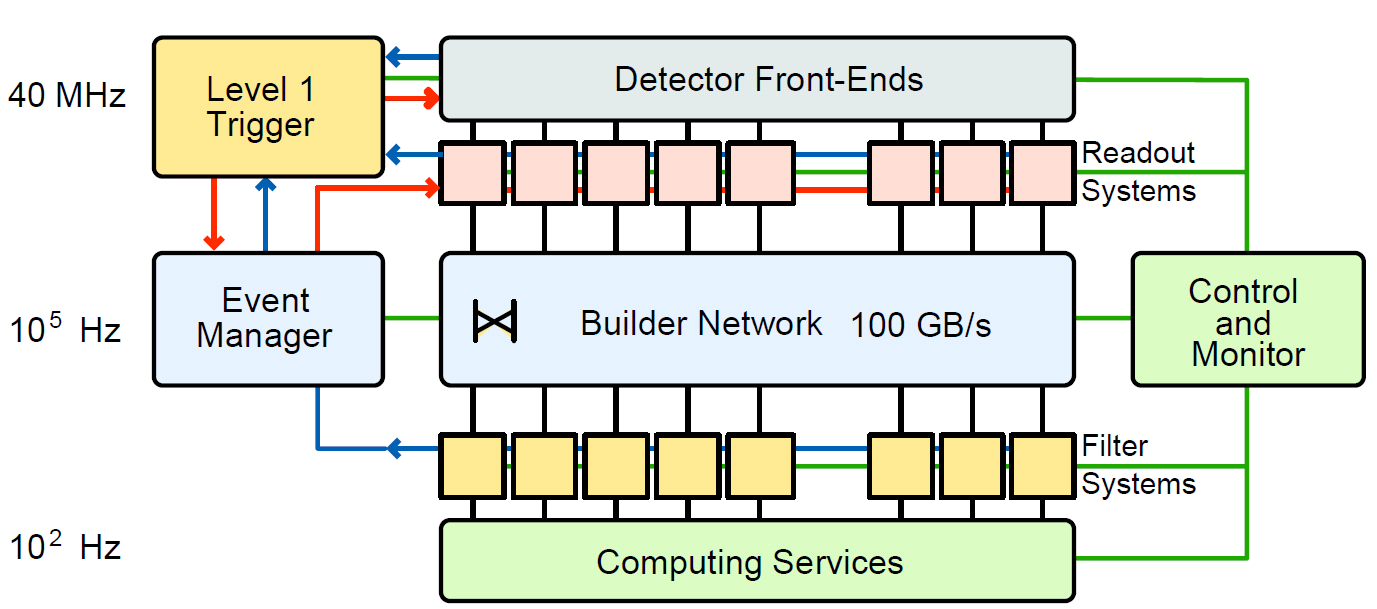
\includegraphics[width=0.80\textwidth]{Chapter02/CMS/Images/CMS_DAQ_Diagram.png}
  \caption{Diagram of the \gls{CMS} \gls{DAQ} system. Data flow is showed as the lines connecting each electronics or computing units \cite{ARTICLE:TheCMSExperiment}.}
  \label{FIGURE:ExperimentalApparatus_CMS_DAQ_Diagram}
\end{figure}

%%%%%%%%%%%%%%%%%%%%%%%%%%%%%%%%%%%%%%%%%%%%%%%%%%%%%%%%%%%%%%%%%%%%%%%%%%%%%%%%%%%%%%%
%%% SUBSECTION
%%%%%%%%%%%%%%%%%%%%%%%%%%%%%%%%%%%%%%%%%%%%%%%%%%%%%%%%%%%%%%%%%%%%%%%%%%%%%%%%%%%%
\subsection{Trigger System}
\label{SUBSECTION:ExperimentalApparatus_CMS_Trigger}

%Status: DONE (needs review)

As described on the previous section the \gls{CMS} trigger system is responsible for selecting which collisions are recorded in real-time. We can only save $10^2-10^3$ events per second with the current systems. This implies that the trigger system needs to obtain a data reduction of a factor of $\mathcal{O}(10^6-10^7)$. This is achieved with a two level trigger system, the first is a dedicated hardware system named \acrfull{L1T} \cite{CMSTDR:CMSTridasTDRVol1} and the second is a commercial computer system running dedicated software called the \acrfull{HLT} \cite{CMSTDR:CMSTridasTDRVol2}.

Initially, all data is stored for 128 bunch crossing which corresponds to $3.2\,\micro\second$. This is the time we have to make a first decision to keep or discard an event. This is the task of the \gls{L1T} which has the target to reduced the data to a maximum rate of $100\,\kilo\hertz$. There isn't enough time to get all the information from the detector, so only a coarse version of the calorimetry and muon systems data, and some correlation between them is accessed. With this information the \gls{L1T} produces a set of particle candidates and energy sums over which custom user defined algorithms can use to filter events. A diagram of the \gls{L1T} trigger components and the data flow across the system is present on figure \ref{FIGURE:ExperimentalApparatus_CMS_L1T_Layout}.

\begin{figure}[!htb]
  \centering
  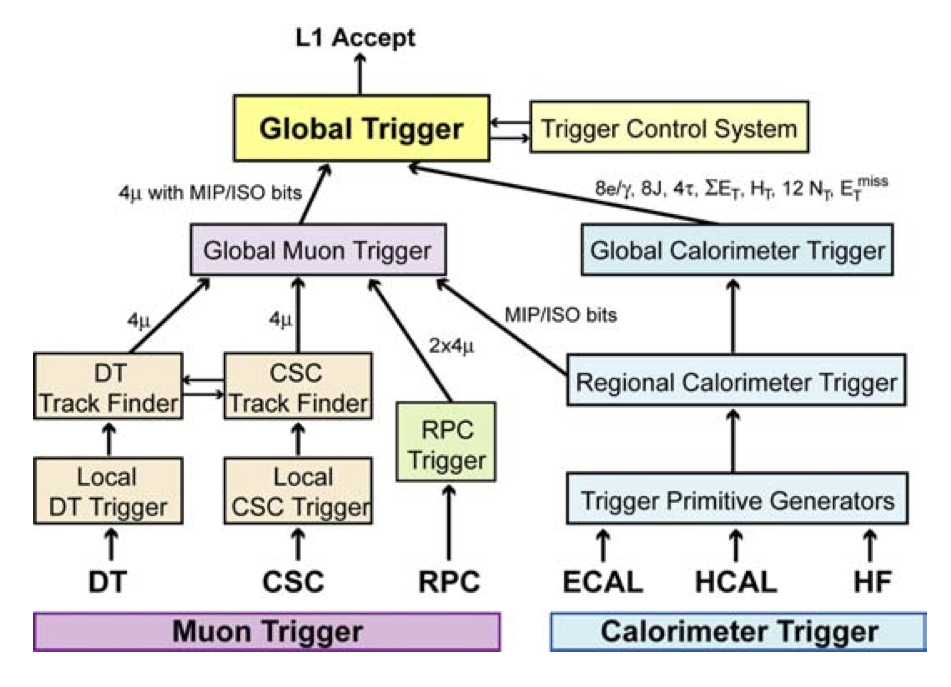
\includegraphics[width=0.80\textwidth]{Chapter02/CMS/Images/CMS_L1T_Layout.png}
  \caption{Diagram of the \gls{L1T} system. The arrows indicate data flow and the number of particle candidates at each step is indicate \cite{ARTICLE:TheCMSExperiment}.}
  \label{FIGURE:ExperimentalApparatus_CMS_L1T_Layout}
\end{figure}

The \gls{HLT} receives events accepted by the \gls{L1T} and needs to perform further event reduction of 
$\mathcal{O}(10^{3}-10^{2})$ to a final output rate of $\mathcal{O}(10^{2-3})\,\hertz$ . This system is composed of standard computing hardware in the form of computing farm with $\approx 15\,\kilo$ \gls{CPU}. This system, using the additional latency created by the \gls{L1T} event selection, is able to make use of the complete detector information including the tracker data. More sophisticated and precise algorithms are therefore possible which can be tailored to select any desired physical final state. 

Event selection algorithms at both the \gls{L1T} and \gls{HLT} are frequently updated during data taking. The selection thresholds may be tuned in order to control the rate with the changes of \gls{LHC} luminosity. Novel methods or strategies to identify particles more efficiently can be implemented, like \gls{PU} subtraction or new calibrations. Analysis groups may also show interest in recording new event final final states for which new selection criteria may be developed. The set of algorithms used for data taking is normally referred as the \textit{trigger menu}. 

After events pass both levels of the trigger they are recorded into permanent storage. During 2012-13 operation, two output streams were saved. The \textit{prompt data stream}, with a rate of approximately $300\,\hertz$, was composed of high priority trigger paths which were immediately reconstructed. And the \textit{parked data stream}, with an average rate of $600\,\hertz$, was stored without reconstruction. This data waited until computing resources were  free to go through reconstruction \cite{ARTICLE:CMSDataParking}. This process was finalised a few months after the \gls{LHC} Run I was finished.

Even with such measures to reduce the data to be stored, each \gls{LHC} experiment records several petabytes of data every year in addition to similarly sized amounts of simulated events.

%%%%%%%%%%%%%%%%%%%%%%%%%%%%%%%%%%%%%%%%%%%%%%%%%%%%%%%%%%%%%%%%%%%%%%%%%%%%%%%%%%%%%%%
%%% SUBSECTION
%%%%%%%%%%%%%%%%%%%%%%%%%%%%%%%%%%%%%%%%%%%%%%%%%%%%%%%%%%%%%%%%%%%%%%%%%%%%%%%%%%%%
\subsection{Computing}
\label{SUBSECTION:ExperimentalApparatus_CMS_Computing}

%Status: DONE

The quantity of data produced by the \gls{LHC} and the necessary processing capability is so big that it would be difficult to have all computing resources in a single place. For this reason a tiered system was developed, where all participating computing sites are connected and have specific roles and responsibilities in the data taking, processing and storing. This global computing system is know as the Grid \cite{CMSTDR:CMSComputing}.

The \gls{CERN} Data Centre is the Tier 0 of this network, all data produced by the \gls{LHC} experiments is handled by this facility. Only about 20\% of the total capacity of the Grid is hosted here, but \gls{CERN} Tier 0 has the very important mission of safe keeping all the raw data produced by the experiments. It also has the task of doing the first attempt of event reconstruction, which is the process identifying meaningful physics objects in data.

There are 7 \gls{CMS} Tier 1 computer centres around the world. They are responsible to store a proportional amount of raw and reconstructed data. If any reprocessing of the data is needed, this centres are responsible for this task and storing the resulting output as well. Tier 1 centres also host simulated data and distribute it to Tier 2 centres. 

Local research centres like universities of scientific laboratories are normally at the Tier 2 level. This centres have the responsibility of handling a proportional share of simulated data production and reconstruction. Currently there are over 150 Tier 2 centres around the world

Individual computers or local clusters without any formal engagement with the Grid structure, are considered to be the Tier 3 level of the Grid. 

%%%%%%%%%%%%%%%%%%%%%%%%%%%%%%%%%%%%%%%%%%%%%%%%%%%%%%%%%%%%%%%%%%%%%%%%%%%%%%%%%%%%%%%
%%% SUBSECTION
%%%%%%%%%%%%%%%%%%%%%%%%%%%%%%%%%%%%%%%%%%%%%%%%%%%%%%%%%%%%%%%%%%%%%%%%%%%%%%%%%%%%
\subsection{Level 1 Trigger: Stage I Upgrade}
\label{SUBSECTION:ExperimentalApparatus_CMS_L1TStage1}

%Status: Writing

An extensive upgrade program for the \gls{L1T} electronics was planed and is being executed in order to cope with the increase of luminosity and pile-up predicted for the period after \gls{LS1} \cite{CMSTDR:CMSL1Upgrade,CMSTDR:CMSUpgradeTDR}. The center-of-mass energy has almost double from $8\,\TeV$ to $13\,\TeV$, instantaneous luminosity will also increase as will average pile-up. Also, the bunch separation has change from $50\,\nano\second$ to $25\,\nano\second$ making out-of-time pile-up a significant problem. 

To ensure physics performance during 2015 and beyond only a partial upgrade was executed for the 2015 run which is known as the \textit{Stage-1} upgrade. The main feature of this upgrade program is the replacement of the existing \gls{GCT}. Two key enhancements were possible: 

\begin{itemize}
  \item Event-by-event pile-up energy subtraction for jets reconstruction, $e/\gamma$ isolation, $\tau$ isolation.
  \item Smaller feature size $\tau$ candidates, which will have significantly better energy estimation and background rejection.
\end{itemize}

The intermediate system will have significantly better performance than the now legacy system. The full 2016 calorimeter trigger system will additionally provide finer granularity which will lead to increased position and energy resolution. 

  \chapter{Technical work}
\label{CHAPTER:TechnicalWork}

\glsresetall % Resetting all acronyms

%Status: DONE

As a member of the \gls{CMS} collaboration it is required that all members perform service work to become full publication authors. For the duration of my Ph.D. program I have fulfilled this requirement within the \gls{L1T} system. This work had a field work component with in the form of \textit{Trigger} and \text{Shift Leader} shifts in the experiment control room, on call shifts as the Trigger \gls{DOC} expert. But also a work as a software developer for the \gls{L1T} \gls{DQM} system. This work lead to my appointment for two years and the coordinator of the software development team. This chapter describes the tools developed and used for online monitoring of the \gls{L1T} during 2012-13 data taking as well as for data certification for physics use.

%%%%%%%%%%%%%%%%%%%%%%%%%%%%%%%%%%%%%%%%%%%%%%%%%%%%%%%%%%%%%%%%%%%%%%%%%%%%%%%%%%%%%%%
%%% SECTION
%%%%%%%%%%%%%%%%%%%%%%%%%%%%%%%%%%%%%%%%%%%%%%%%%%%%%%%%%%%%%%%%%%%%%%%%%%%%%%%%%%%%%%%
\section{Data Quality Monitoring}
\label{SECTION:TechnicalWork_DataQualityMonitoring}

%Status: DONE

The \acrfull{DQM} is a critical monitoring system that has an important role in detector and operations efficiency, and certification of recorded data for physics analysis \cite{CMSTDR:CMSTridasTDRVol1,ARTICLE:CMSDataQualityMonitoringSoftWare_ExperienceAndFuture}. The \gls{DQM} system is an end-to-end solution that provides tools to create, fill, display and archive histograms and scalar monitors. It provided the ability to monitor the detector and \gls{DAQ} in real-time, analyse the reconstruction process, validate the experiment software releases and its simulated data. The purpose of this system is to identify problems or errors in both hardware and software as early and accurately as possible.

%%%%%%%%%%%%%%%%%%%%%%%%%%%%%%%%%%%%%%%%%%%%%%%%%%%%%%%%%%%%%%%%%%%%%%%%%%%%%%%%%%%%%%%
%%% SUBSECTION
%%%%%%%%%%%%%%%%%%%%%%%%%%%%%%%%%%%%%%%%%%%%%%%%%%%%%%%%%%%%%%%%%%%%%%%%%%%%%%%%%%%%%%%
\subsection{Online Monitoring}
\label{SECTION:TechnicalWork_DataQualityMonitoring_OnlineMonitoring}

%Status: DONE

The online \gls{DQM} system is composed of several applications that are part of the \gls{CMS} data processing work flow. The software is execute at the \gls{CMS} point 5 computing cluster and applications fall into two categories: \textit{high level trigger modules} and \textit{data quality monitoring modules}. The \textit{high level trigger modules} are run directly in the \gls{HLT} filter farm and can only produce a limited number of histograms with the purpose of monitoring this system or specific \gls{HLT} path. The \textit{data quality monitoring modules} run on a dedicated \gls{DQM} event stream with a rate of $5-10\,\hertz$. These events contain the raw detector and trigger information. Each subsystem has its own application which can analyse all events from the stream or filter a subset with a predefined trigger selection. At the end of every luminosity section, which corresponds to $23.31\,\second$, histograms are gathered from the nodes where the applications are running and merged. The results are showed in real time in a web based application which is accessible by the shift crew and on call experts.

%%%%%%%%%%%%%%%%%%%%%%%%%%%%%%%%%%%%%%%%%%%%%%%%%%%%%%%%%%%%%%%%%%%%%%%%%%%%%%%%%%%%%%%
%%% SUBSECTION
%%%%%%%%%%%%%%%%%%%%%%%%%%%%%%%%%%%%%%%%%%%%%%%%%%%%%%%%%%%%%%%%%%%%%%%%%%%%%%%%%%%%%%%
\subsection{Offline Monitoring}
\label{SECTION:TechnicalWork_DataQualityMonitoring_OfflineMonitoring}

%Status: DONE

The offline \gls{DQM} is used in numerous workflows including monitoring of the event reconstruction process, alignment and calibration validation, \gls{CMS} software release validation, etc. For all this task a standardized two step process is run. 

In the first step histograms are produced in the same computing jobs of the task to be monitored and stored along with the rest of the event data. This is happens in multiple simultaneous jobs which depending on the task can be at Tier 0 or Tier 1 level.

In the second \textit{harvesting step}, the histograms are extracted from the event data and summed together. The resulting histograms contain the full event yields from each run for each processed dataset. Application running at the step have access to the detector conditions from \gls{DCS} and \gls{DAQ} conditions and can produce new histograms such as summaries of the relevant quantities for each run.

%%%%%%%%%%%%%%%%%%%%%%%%%%%%%%%%%%%%%%%%%%%%%%%%%%%%%%%%%%%%%%%%%%%%%%%%%%%%%%%%%%%%%%%
%%% SECTION
%%%%%%%%%%%%%%%%%%%%%%%%%%%%%%%%%%%%%%%%%%%%%%%%%%%%%%%%%%%%%%%%%%%%%%%%%%%%%%%%%%%%%%%
\section{Level 1 Trigger Data Quality Monitoring}
\label{SECTION:TechnicalWork_L1TDQM}

%Status: Writting

The \acrfull{L1T} \acrfull{DQM} is composed of four applications. The first two application run as a part of the online \gls{DQM} system with the mission of monitoring the trigger and trigger emulation in real-time. The second pair of application runs in the offline \gls{DQM} system as part of the (re-)reconstruction workflow with the main function of providing information for physics data certification.

First of the two online applications directly monitors the operation of the trigger. Each trigger subsystem produces plots over the produced objects or relevant quantities which allow to pin-point the origin of problems. Additionally, global trigger operation is monitored in key aspect such as the value of reference algorithm rates, synchronization of firing, finding regions of the detector that fires with unexpectedly high/low rate. The second online application compares the results of the trigger against a real-time software emulation of the system which should allow quick detection of trigger miss configuration or degradation of quality of operation.

Both offline monitoring applications replicate the analysis preformed by their online counterparts but over a the complete recorded dataset for each run.

In the next sections we will focus only on the trigger monitoring tools that the author developed or improved.

%%%%%%%%%%%%%%%%%%%%%%%%%%%%%%%%%%%%%%%%%%%%%%%%%%%%%%%%%%%%%%%%%%%%%%%%%%%%%%%%%%%%%%%
%%% SUBSECTION
%%%%%%%%%%%%%%%%%%%%%%%%%%%%%%%%%%%%%%%%%%%%%%%%%%%%%%%%%%%%%%%%%%%%%%%%%%%%%%%%%%%%%%%
\subsection{Rates Monitoring}
\label{SECTION:TechnicalWork_L1TDQM_RatesMonitoring}

%Status: DONE

The rates monitoring tool has the objective of inspecting the firing rate of each \gls{L1T} object category. At the beginning of each run the \gls{L1T} menus is analysed and for each object category the lowest thresholds unprescaled algorithm is selected. If no unprescaled algorithm is available the lowest prescale algorithm is selected. The following categories of objects can be monitored: Electron-Gamma, Isolated Electron-Gamma, Central Jets ($|\eta|<3$), Forward Jets ($3<|\eta|<5$), All Jets ($|\eta|<5$), Taus, Muon, total energy (ETT), total energy in jets (HTT), missing energy (ETM) and jets missing energy (HTM).

When the algorithms to be monitored are determined the tool retrieves from an external database the expected algorithm cross section as a function of instantaneous luminosity. This function are updated daily by fitting runs from the previous days with similar condition. This task is executed by the \gls{WbM} system which is a \gls{CMS} monitoring system which runs in parallel to the \gls{DQM}. The algorithm cross section for each luminosity section calculated is calculated with following equation \ref{EQUATION:TechnicalWork_AlgoCrossSection}.

\begin{equation}
\sigma_{\text{Algo}}=\frac{\text{Prescale}_{\text{Algo}}*{\text{Avg. Rate}_{\text{Algo}}}}{\text{Avg. Instantaneous Luminosity}}
\label{EQUATION:TechnicalWork_AlgoCrossSection}
\end{equation}

For each luminosity section the measured value is compared with prediction from previous runs. The monitor presents this results in histograms with the measured value and the relative value to prediction. An example of this histograms can be found in figure \ref{FIGURE:TechnicalWork_RateMonitoring}

\begin{figure}[!htb]
\centering
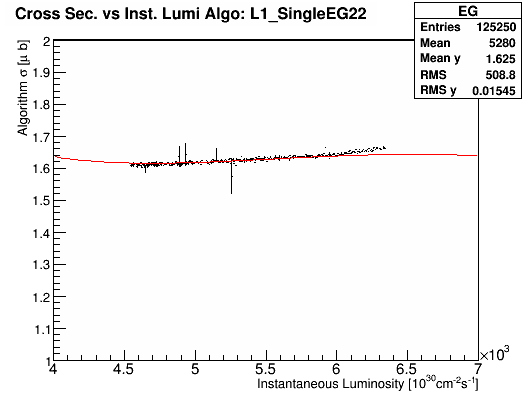
\includegraphics[width=0.45\textwidth]{Chapter03/L1TOnline/Images/L1TDQM_Online_Run207269_L1TRate_TriggerCrossSections_EG.png}
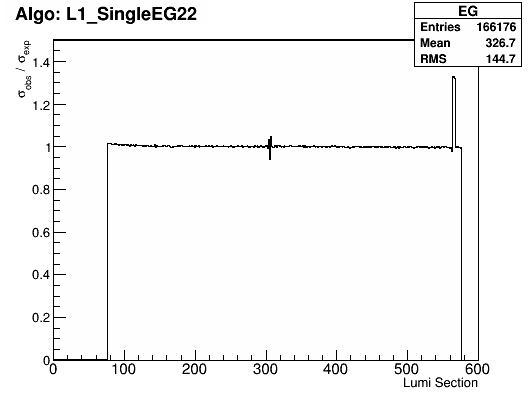
\includegraphics[width=0.45\textwidth]{Chapter03/L1TOnline/Images/L1TDQM_Online_Run207269_L1TRate_Certification_EG.png}
\caption{Monitoring plots produced by the \gls{L1T} online rates monitoring tool for run 207269 and the Electron-Gamma object category. The automatically selected algorithm was L1\_SingleEG22 for this run. On the left histogram the the algorithm cross section as a function of instantaneous luminosity is plotted. The red line is the prediction from fitting data from previous runs while the black points are the measurements for this run. On the right histogram the fraction of the measured value to the prediction is showed for each luminosity section.}
\label{FIGURE:TechnicalWork_RateMonitoring}
\end{figure}

Automatic tests are configured to monitor the produced histograms and flag as bad luminosity sections that show deviation from prediction above 20\%. Marking a specific luminosity section as bad does not invalidate automatically its use for physics analysis but references it for further investigation by the \gls{CMS} shift crew or certification experts.

%%%%%%%%%%%%%%%%%%%%%%%%%%%%%%%%%%%%%%%%%%%%%%%%%%%%%%%%%%%%%%%%%%%%%%%%%%%%%%%%%%%%%%%
%%% SUBSECTION
%%%%%%%%%%%%%%%%%%%%%%%%%%%%%%%%%%%%%%%%%%%%%%%%%%%%%%%%%%%%%%%%%%%%%%%%%%%%%%%%%%%%%%%
\subsection{Synchronization Monitoring}
\label{SECTION:TechnicalWork_L1TDQM_SynchronizationMonitoring}

%Status: Writting

This tool was initially developed by me during last year and now has been improved and debugged. It monitors
the synchronization of the lowest unprescaled single object trigger of all available L1 trigger object categories
by looking at \gls{HLT} pass-through paths events (no selection at \gls{LHC} to avoid bias) and looking at the 5 bunch crossing
L1 trigger information provided by the GT. The trigger records can then be compared with the published LHC bunch
structure and a fraction of in time events can be calculated. New developments include alteration in the way
information is retrieved from the database and avoiding the use of \gls{HLT} pass-throughs and therefore improving statistics
by looking at events from an object category seeded by an independent object category. As an example: single muon
trigger can seed calorimeter triggers synchronization tests.

\begin{figure}[!htb]
\centering
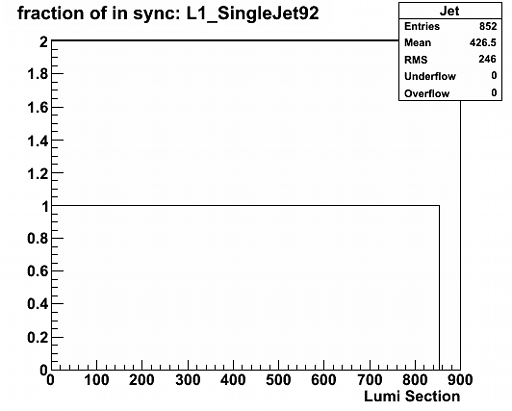
\includegraphics[width=0.45\textwidth]{Chapter03/L1TOnline/Images/Run177878_Jet_SynchronizationCertification.png}
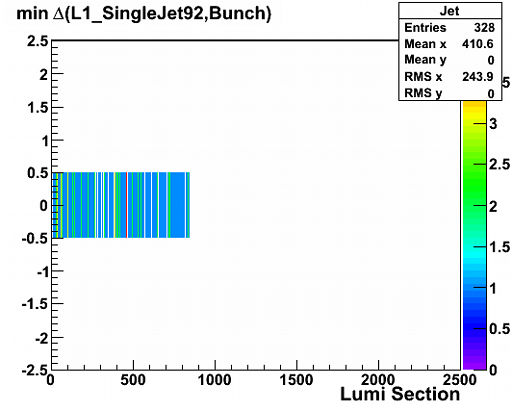
\includegraphics[width=0.45\textwidth]{Chapter03/L1TOnline/Images/Run177878_Jet_SynchronizationTest.png}
\caption{Monitoring plot produced by the L1TSync tool for L1 single electron/gamma object category, which is
automatically monitoring algorithm L1\_SingleEG50 for the run 177878. In the plots data points are the calculated
trigger cross section as a function of instant luminosity and the line is the reference fit done from previous runs.}
\label{figure_ServiceWork_L1TSync}
\end{figure}

%%%%%%%%%%%%%%%%%%%%%%%%%%%%%%%%%%%%%%%%%%%%%%%%%%%%%%%%%%%%%%%%%%%%%%%%%%%%%%%%%%%%%%%
%%% SUBSUBSECTION
%%%%%%%%%%%%%%%%%%%%%%%%%%%%%%%%%%%%%%%%%%%%%%%%%%%%%%%%%%%%%%%%%%%%%%%%%%%%%%%%%%%%%%%
\subsubsection{BPTX Monitoring}

%Status: Writting

This tool was created during August 2012 to meet a concern of the \gls{L1T} trigger management. It monitors the \gls{BPTX} system by looking at the information present at each event that 
is analyzed by the \gls{DQM} system, including the 2 bunch crossings before and after the actual event that fired. Then it 
compares where the \gls{BPTX} fired on those 5 bunch crossings with the LHC published bunch structure. The \gls{BPTX} efficiency 
and misfire rate are calculated and the rate stability is also monitored.

%%%%%%%%%%%%%%%%%%%%%%%%%%%%%%%%%%%%%%%%%%%%%%%%%%%%%%%%%%%%%%%%%%%%%%%%%%%%%%%%%%%%%%%
%%% SUBSECTION
%%%%%%%%%%%%%%%%%%%%%%%%%%%%%%%%%%%%%%%%%%%%%%%%%%%%%%%%%%%%%%%%%%%%%%%%%%%%%%%%%%%%%%%
\subsection{Implementation Tests}

%Status: Writting

\begin{figure}[!htb]
\centering
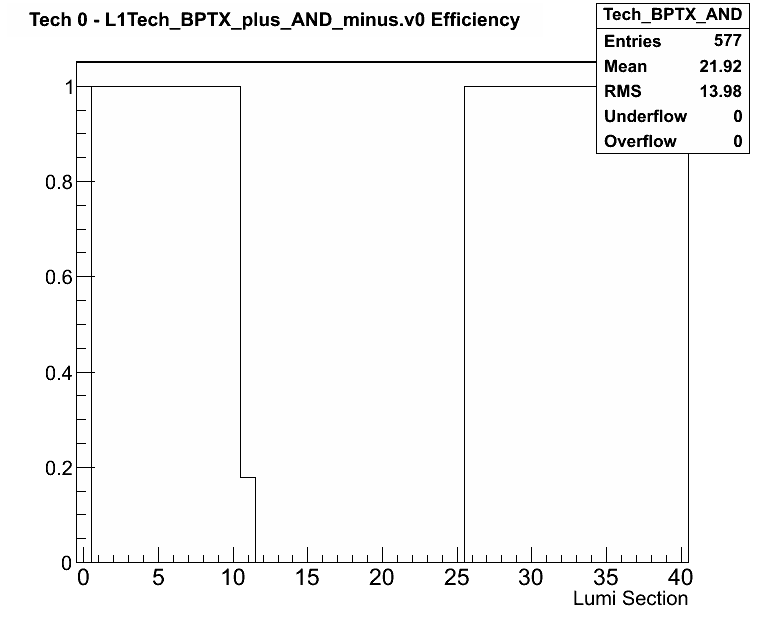
\includegraphics[width=0.45\textwidth]{Chapter03/L1TOnline/Images/L1TBPTX_Tech_BPTX_AND.png}
\caption{Monitoring plot produced by the L1TBPTX tool for the run 207269 where a test was executed to demonstrate that 
this tools works. In the plot the BPTX AND (technical algorithm 0) efficiency is calculated per luminosity section 
when compared with the LHC published bunch structure. The dip in efficiency corresponds to the disabling of the BPTX 
related triggers.} 
\label{figure_ServiceWork_L1TBPTX}
\end{figure}

%%%%%%%%%%%%%%%%%%%%%%%%%%%%%%%%%%%%%%%%%%%%%%%%%%%%%%%%%%%%%%%%%%%%%%%%%%%%%%%%%%%%%%%
%%% SUBSECTION
%%%%%%%%%%%%%%%%%%%%%%%%%%%%%%%%%%%%%%%%%%%%%%%%%%%%%%%%%%%%%%%%%%%%%%%%%%%%%%%%%%%%%%%
\subsection{Occupancy Monitoring}

%Status: Writting

This tool was developed initially by me in collaboration with a CERN summer student during last year and has been
also improved and debugged. It monitors several key occupancy plots from L1 subsystems, by making use of the natural
$\eta-\phi$ symmetry normally present. It compares each cell to the median of a strip in $\phi$ in the opposite $\eta$
side of the detector, by applying a $\chi^{2}$ like test tuned to fire when the cell is less than 10\% or more than
twice the value of the reference median. New developments include the inclusion of new plots which comply with the
tools specifications (provided by the sub-systems) and include the possibility of masking strips from the test, which 
will make the tool compare the cell with the median of the $\phi$ strip where it is included.

\begin{figure}[!htb]
\centering
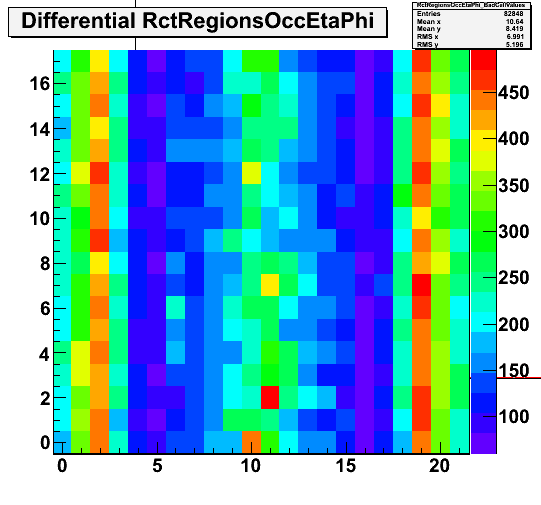
\includegraphics[width=0.45\textwidth]{Chapter03/L1TOnline/Images/L1TOccupancy_Diff.png}
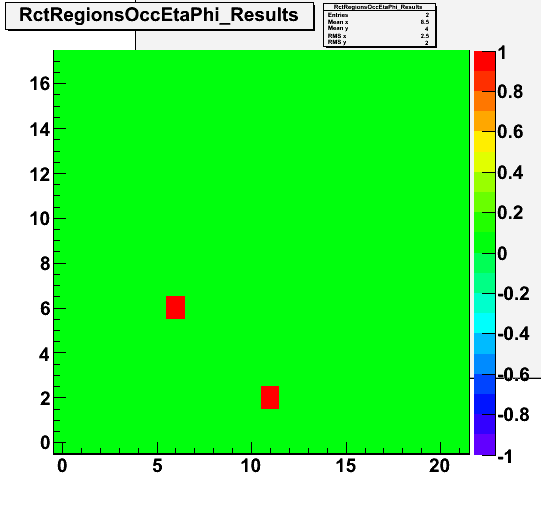
\includegraphics[width=0.45\textwidth]{Chapter03/L1TOnline/Images/L1TOccupancy_Results.png}
\caption{Monitoring plot produced by the L1TOccupancy tool for the run 207099 while testing GCT plot for isolated
EM occupancy $\eta-\phi$. In blue are the masked bins, in green the cells that pass the test and in red the cells
that fail the test. The cells marked as bad are in fact a consequence of the initial plot being produced without
a cut on minimum $p_T$ on the trigger primitives, so the asymmetries observed are due to pedestal differences between
difference areas.}
\label{figure_ServiceWork_L1TOccupancy}
\end{figure}

\section{Status Summary Display}

%Status: Writting

\begin{figure}[!htb]
\centering
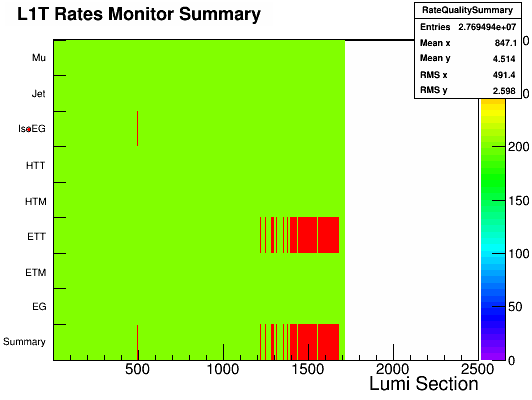
\includegraphics[width=0.45\textwidth]{Chapter03/L1TOnline/Images/RateQualitySummary.png} 
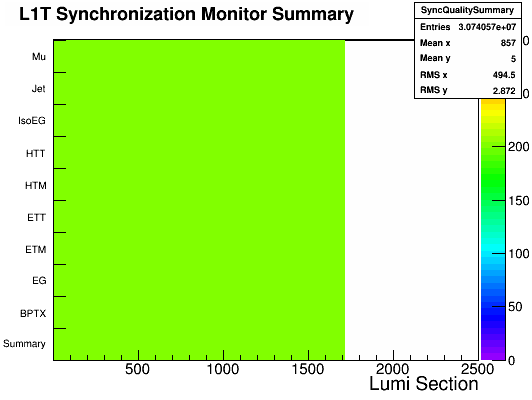
\includegraphics[width=0.45\textwidth]{Chapter03/L1TOnline/Images/SyncQualitySummary.png} \\
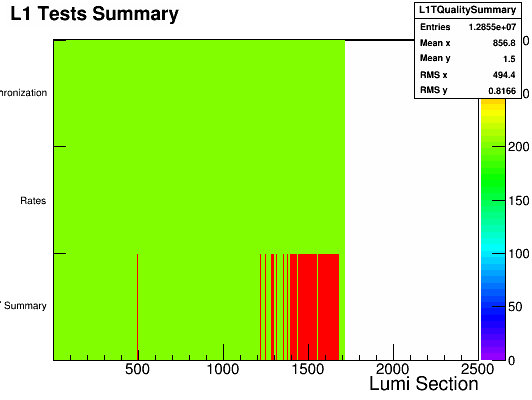
\includegraphics[width=0.45\textwidth]{Chapter03/L1TOnline/Images/L1TQualitySummary.png}
\caption{}
\label{figure_ServiceWork_StatusSummary}
\end{figure}

%%%%%%%%%%%%%%%%%%%%%%%%%%%%%%%%%%%%%%%%%%%%%%%%%%%%%%%%%%%%%%%%%%%%%%%%%%%%%%%%%%%%%%%
%%% SUBSECTION
%%%%%%%%%%%%%%%%%%%%%%%%%%%%%%%%%%%%%%%%%%%%%%%%%%%%%%%%%%%%%%%%%%%%%%%%%%%%%%%%%%%%%%%
\subsection{Certification}

%Status: Writting

% \section{Proposed Future Upgrades}

  \chapter{Physics Objects and Monte Carlo simulation}

\section{Physics objects definition}

\subsection{Electron}

\subsection{Muon}

\subsection{Tau}

\subsection{Jets}

\subsection{Missing Transverse Energy}

\section{Monte Carlo simulation}



% \clearpage
% \section{Introduction}

The search for an invisible decay of a vector boson produced Higgs boson was first made public with CMS Physics Analysis Summary (PAS) HIG-13-013 which was further improved and combined with other Higgs boson production channel in the CMS paper HIG-13-30. Additional support material can be found at the CMS Analysis Notes (AN) AN-2012/403\cite{CMS_AN_2013-403} and AN-2013/205.

During the 2012 data taking run two main streams of data were recorded. The main stream with an event rate of the order of 300 Hz to be promptly reconstructed and made available for analysis in a few days after being recorded, this dataset is referred to as the prompt data. The secondary stream with lower trigger thresholds with an event rate of the order of 1kHz which would only be reconstructed when the computing resources would be available outside of the data taking period, dataset is referred to as parked data. Our previous results
were produced using the prompt data only and this work now extends on previous work by using the now available parked data. Since this dataset has been recorded with lower trigger thresholds the analysis was re-optimised to take advantage of this new available phase space. The details of the newly developed analysis can be found in CMS AN-14-243\cite{CMS_AN_2014-243}.

It is normally a requirement for many CMS publications to have a cross check analysis implemented independently from the main result in order to be able to ensure accuracy of the final results due to possible errors with the software implementation. For this purpose the previous prompt data VBF Higgs to Invisible results and publication were produced by two different and independent code frameworks and before publication a good level of synchronization were obtained. Due to lack of man power and time it was decide for the 2012 parked data analysis to only proceed with a single framework. At a later stage of the analysis it was thought that at least some level of cross check would be a good measure to limit the possibility of implementation errors and to allow extra confidence on the final results.

This cross check analysis starts from the same ntuples produced by the main analysis which were produced over all the relevant datasets and are recorded with data formats also used by other analysis at Imperial College London, e.g. both the SM and MSSM Higgs to $\tau\bar{\tau}$, the Higgs to $\tau\bar{\tau}b\bar{b}$ and prompt Higgs to invisible analyses. No cuts are applied at ntuple production except the official CMS selection for good usable data using the appropriate golden JSON file.

From those initial ntuple an independent code framework was developed in order to replicate all relevant numbers and plots from the main analysis.

% \section{Data samples}

For this analysis we used the proton-proton collision parked data collected by the CMS experiment during 2012-13. An analysis purposely constructed trigger was used to collect this data.

\begin{table}[htp]
\centering

\begin{tabular}{|l|c|}
\hline
Dataset & $\int{Luminosity}$ $[pb^{-1}]$ \\
\hline \hline
/MET/Run2012A-22Jan2013-v1/AOD        & 889 \\
/VBF1Parked/Run2012B-22Jan2013-v1/AOD & 3871 \\
/VBF1Parked/Run2012C-22Jan2013-v1/AOD & 7152 \\
/VBF1Parked/Run2012D-22Jan2013-v1/AOD & 7317 \\
\hline
Total analysed & 19229 \\
\hline \hline
Total certified luminosity & 19789 \\
\hline
\end{tabular}

\caption{Used datasets and their respective integrated luminosities after applying certified for physics filtering. Each dataset corresponds to a recording period/era of the 2012-13 data acquisition run.}
\end{table}

% Review text abouve

% To include
% * Explain breifly the validadion process (JSON)
% * Table with data included


% \section{Event Filters and object definitions}

%STATUS: Finished
%TODO: 
% * Could not find any reference to this recommendations!
\subsection{Vertex}

The interaction point is normally assumed to be the reconstructed  primary vertex, defined as the vertex with highest sum of associated tracks \pt squared, or if that cannot be determined the beam spot position is assumed. Knowing precisely the interaction point will allow to determine object quantities relative to it which allow for better object identification and pile-up control. At least one good vertex implicitly required by tracking failure event quality filter. And Additionally we require explicitly that a good vertex is reconstructed with the following characteristics. 

\begin{itemize}
  \item NOT(isFake): We require a real reconstructed vertex from tracks, not the beam spot.
  \item Number of degrees of freedom: $n_{dof}>4$
  \item Longitudinal distance: $|z|<=24$
  \item Radial distance to beam line: $d_{xy}<2$
\end{itemize}

%STATUS: Finished
%TODO: 
% * Add citation for the Jet-MET POG for this filter usage (include data and page version)
% * QUESTION: Should I include description of what each filter does?
\subsection{Event quality filters}

During data recording issues may happen with the detector or acquisition which may render some of the events unusable. The groups responsible for each part of the detector and physics object check the data after and was taken and if they find such problems software event filters are made available for analysis to be able to remove this problematic events. This event filters will address issues like detector know problems, miss firing of calibration sequences or failure to reconstruct physics objects. The Jet-MET Particle Object Group (POG) recommends the usage of the following filters which are used in this analysis\cite{CMS:JetMETPOG:MissingETOptionalFilters}.

\begin{itemize}
  \item CSCTightHaloFilter
  \item HBHENoiseFilter
  \item EcalDeadCellTriggerPrimitiveFilter
  \item trackingFailureFilter
  \item eeBadScFilter
  \item ECAL Laser filter (via event list)
  \item HCAL Laser filter (via event list)
\end{itemize}

In turn the JetMET group recommend the usage of the following Tracking POG Filter\cite{CMS:TrackingPOG:TrackingPOGFilters}:

\begin{itemize}
  \item  logErrorTooManyClusters
  \item  manystripclus53X
  \item  toomanystripclus53X
\end{itemize}

The event rejection efficiencies from the all filters except ECAL and HCAL laser event filters can be found at table \ref{table_EventQualityFilterEff}. This values are measured the vertex requirements. 

\begin{table}[!htp]
\centering

\begin{tabular}{|l||c|c|c|c|}
\hline
Filter                  & Prompt A & Parked B & Parked C & Parked D \\
\hline \hline
ECAL Laser Filter       & 0.928521 & 0.008659 & 0.000000 & 0.000000 \\
HCAL Laser Filter       & 0.007258 & 0.000000 & 0.000270 & 0.000000 \\
\hline
ECAL+ HCAL Laser Filter & 0.935704 & 0.008659 & 0.000270 & 0.000000 \\
\hline
\end{tabular}

\caption{Event rejection efficiency for the ECAL and HCAL Laser Filters. This events have to be removed due to the untimely firing of the calibration laser for this systems.}
\label{table_CaloLaserFilterEff}
\end{table}


The values for the ECAL and HCAL laser event filters are present in table \ref{table_CaloLaserFilterEff}. This value are calculated after vertex requirement and the filters in table \ref{table_EventQualityFilterEff}. 

\begin{table}[htp]
\centering

\begin{tabular}{|l||c|c|c|c|}
\hline
Filter                             & Prompt A  & Parked B & Parked C & Parked D \\
\hline \hline
HBHENoiseFilter                    & 22.900905 & 0.190670 & 0.187739 & 0.170753 \\
EcalDeadCellTriggerPrimitiveFilter &  0.375381 & 0.009300 & 0.010206 & 0.012526 \\
eeBadScFilter                      &  0.007852 & 0.000001 & 0.000000 & 0.000009 \\
trackingFailureFilter              &  3.073876 & 0.000328 & 0.007464 & 0.000290 \\
manystripclus53X                   &  0.001829 & 0.001319 & 0.002335 & 0.001327 \\
toomanystripclus53X                &  0.000484 & 0.001149 & 0.002006 & 0.001173 \\
logErrorTooManyClusters            &  0.000027 & 0.000009 & 0.000021 & 0.000016 \\
CSCTightHaloFilter                 & 10.263068 & 0.398497 & 0.402936 & 0.508025 \\
\hline
Total                              & 28.501208 & 0.598417 & 0.601999 & 0.689380 \\
\hline
\end{tabular}

\caption{Percentage of events in data failing each of the event quality filters after requesting on good vertex. For the parked analysis we use prompt A and parked B, C and D datasets.}
\label{table_EventQualityFilterEff}
\end{table}

It is observed that the HBHENoiseFilter vetos around 22\% of the event for prompt run A but this behaviour is not observed in any of the parked datasets. This specific filter removed events with noise in the HCAL. An example of noise would be a ``hot tower'' reading very high energy values, some times for several events. Since this energy will not be balance in each event this will greatly increase \MET. On the prompt dataset there are \MET only triggers which were fired in such events which then get removed by this filter, those triggers are not present in parked dataset. This can clearly be seen if we apply first our trigger selection (Jets+\MET) and then recalculate the event rejection efficiencies, this values can be found in table \ref{table_EventQualityFilterEff_PostTrigger}.

\begin{table}[htp]
\centering

\begin{tabular}{|l||c|c|c|c|}
\hline
Filter                             & Prompt A & Parked B & Parked C & Parked D \\
\hline \hline
HBHENoiseFilter                    & 1.264571 & 0.186895 & 0.178422 & 0.154080 \\
EcalDeadCellTriggerPrimitiveFilter & 0.572468 & 0.010081 & 0.010338 & 0.010725 \\
eeBadScFilter                      & 0.000989 & 0.000001 & 0.000000 & 0.000000 \\
trackingFailureFilter              & 0.062289 & 0.000401 & 0.009729 & 0.000231 \\
manystripclus53X                   & 0.002966 & 0.001264 & 0.002304 & 0.001255 \\
toomanystripclus53X                & 0.002966 & 0.001093 & 0.001955 & 0.001103 \\
logErrorTooManyClusters            & 0.000000 & 0.000000 & 0.000000 & 0.000000 \\
CSCTightHaloFilter                 & 0.400431 & 0.397531 & 0.403156 & 0.506917 \\
\hline                             
Total                              & 2.201877 & 0.594332 & 0.592977 & 0.671026 \\
\hline
\end{tabular}

\caption{Percentage of events in data failing each of the event quality filters after requesting on good vertex and trigger conditions. For the parked analysis we use prompt A and parked B, C and D datasets.}
\label{table_EventQualityFilterEff_PostTrigger}
\end{table}

Both tables \ref{table_EventQualityFilterEff} and \ref{table_CaloLaserFilterEff} can be directly compared with the values produced by the main analysis and presented in AN-14-243\cite{CMS_AN_2014-243}. No differences are observed.

%STATUS: In progress
%TODO:  
\subsection{Jets}

In this analysis we use particle flow  jets clustered with the $anti-k_{T}$ algorithm with a cone size of 0.5. 

The correction L1FastJet, L2Relative and L3Absolute are applied to both data and monte carlo (MC) and additionally we apply L2L3Residual to data.

The to correct Jet Energy Scale we apply global tag FT53\_V21A\_AN6::All for data and START53\_V27::All for monte carlo.

The jets with this characteristics and corrections are available in the ntuples produced by the main analysis as the "standard" jets collection. We further require that our selected jets pass PFJet ID and pileup ID. And we clean the jet collection by removing all jets that closer then $\Delta R < 0.5$ to any veto electron or loose muon (relevant for control regions).

%Out of this jets we select the ones passing loose PFJet ID and pileup ID. We also clean the jet collection by removing all jets that closer then %$\Delta R < 0.5$% to any veto electron or loose muon (relevant for control regions).
 
%% FOR MY PHD THESIS 
%% Details on 
%  
% As a selection condition for out jets we use the PFJet ID described at [[CMS/JetID.Recommendations_for_8_TeV_data_a][JetID page]].
% 
% The jet requirements are:
%    * Neutral Hadron Fraction %$ <0.99 $%
%    * Neutral EM Fraction %$ <0.99 $%
%    * Number of Constituents  %$ >1 $%
% Additionally for %$|\eta| < 2.4$% we require:
%    * Charged Hadron Fraction %$  >0 $%
%    * Charged Multiplicity %$ >0 $%
%    * Charged EM Fraction %$ 0.99 $%
% 
% ---+++ Pileup ID 
% 
% Using the prescription at the [[CMS.PileupJetID][PileupJetID page]] we reject pileup jets cutting at loose working point of a BDT with Dec2012 weights and package recojets/jetproducers with version METPU_5_3_X_v4. The computation of the MVA value per jet is made when the ntuples are produced and this values are stored within each jet. We cut on the BDT score categorizing in %$p_{\perp}$% and %$|\eta|$% as follows:
% 
% %BEGINLATEX%
% \begin{tabular}{|c|c|c|}
% \hline
% Jet $p_{\perp}$ & Jet $|\eta|$ & $BDT_{score}$ \\
% \hline \hline
% $20 < p_{\perp} \leq 30$ & $|\eta| < 2.5$ & $BDT_{score} > -0.80$ \\
% $20 < p_{\perp} \leq 30$ & $2.50 \leq |\eta| < 2.75$ & $BDT_{score} > -0.85$ \\
% $20 < p_{\perp} \leq 30$ & $2.75 \leq |\eta| < 3.00$ & $BDT_{score} > -0.84$ \\
% $20 < p_{\perp} \leq 30$ & $3.00 \leq |\eta| < 5.00$ & $BDT_{score} > -0.85$ \\
% $30 < p_{\perp}$ & $|\eta| < 2.5$ & $BDT_{score} > -0.80$ \\
% $30 < p_{\perp}$ & $2.50 \leq |\eta| < 2.75$ & $BDT_{score} > -0.74$ \\
% $30 < p_{\perp}$ & $2.75 \leq |\eta| < 3.00$ & $BDT_{score} > -0.68$ \\
% $30 < p_{\perp}$ & $3.00 \leq |\eta| < 5.00$ & $BDT_{score} > -0.77$ \\
% \hline
% \end{tabular}
% %ENDLATEX%

%STATUS: In progress
%TODO:  
\subsection{Missing transverse energy \texorpdfstring{(\MET)}{}}


%STATUS: In progress
%TODO: 
% Convert base cut based ID to a table  
\subsection{Electrons}

% Make citation for CMS.EgammaCutBasedIdentification
For this analysis we use two categories of electrons "veto electrons" and "tight electrons". Both this categories of particles are based on standard EGamma POG cut based object definition which can be found at (TODO:CITATION). Additionally, we require some additional cuts to each category (TODO:WHY).

\subsubsection{Veto electrons}
 
The "veto electrons" are defined by the base requirements of the cut based electron ID veto working point of the EGamma POG with some additional cuts on top. 
 
Requirements of the cut based electron ID veto working point:

Barrel Cuts ( $ |\eta_{supercluster}|<=1.479 $ )
\begin{itemize}
  \item $ | \Delta\eta(track,supercluster) | < 0.007 $
  \item $ | \Delta\phi(track,supercluster) | < 0.8 $
  \item $ \sigma(i\eta,i\eta) < 0.01 $
  \item $ H/E < 0.15 $
  \item $ |d_{0}(vertex)| < 0.04 $
  \item $ |d_{Z}(vertex)| < 0.2 $
  \item $ \frac{PF_{isolation}}{p_{\perp}} < 0.15 $ for $ \Delta R_{cone}=0.3 $
\end{itemize}

Endcap Cuts ( $ 1.479 < |\eta_{supercluster}| < 2.5 $ )
\begin{itemize}
  \item $ | \Delta\eta(track,supercluster) | < 0.1 $
  \item $ | \Delta\phi(track,supercluster) | < 0.7 $
  \item $ \sigma(i\eta,i\eta) < 0.03 $
  \item $ |d_{0}(vertex)| < 0.04 $
  \item $ |d_{Z}(vertex)| < 0.2 $
  \item $ \frac{PF_{isolation}}{p_{\perp}} < 0.15 $ for $ \Delta R_{cone}=0.3 $
\end{itemize}

Additional requirements for this analysis
\begin{itemize}
  \item $ p_{\perp} > 10 $ GeV
  \item $ |\eta| < 2.4 $
  \item $ Effective-Area-Corrected-Isolation < 0.15 $ (is stated in the note as additional requirement but does not look like it is)
  \item $d_{xy}<0.04$ cm (is stated in the note as additional requirement but does not look like it is)
  \item $d_{z} < 0.2 $ cm (is stated in the note as additional requirement but does not look like it is)
\end{itemize}

\subsubsection{Tight electrons}

The "tight electrons" are defined by using the base requirements of the cut based electron ID tight working point (similar to 2011 very tight WP70) of the EGamma POG with some additional cuts on top.
 
Requirements of the cut based electron ID tight working point (similar to 2011 very tight WP70):

Barrel Cuts ( $ |\eta_{supercluster}|<=1.479 $ )
\begin{itemize}
  \item $ | \Delta\eta(track,supercluster) | < 0.004 $
  \item $ | \Delta\phi(track,supercluster) | < 0.3  $
  \item $ \sigma(i\eta,i\eta) < 0.01 $
  \item $ H/E < 0.12 $
  \item $ |d_{0}(vertex)| < 0.02 $
  \item $ |d_{Z}(vertex)| < 0.1 $
  \item $ |\frac{1}{E}-\frac{1}{p}| < 0.05 $
  \item $ \frac{PF_{isolation}}{p_{\perp}} < 0.10 $ for $ \Delta R_{cone}=0.3 $
  \item Conversion rejection: vertex fit probability: 1e-6
  \item Conversion rejection: missing hits $<= 0$
\end{itemize}

Endcap Cuts ( $ 1.479 < |\eta_{supercluster}| < 2.5 $ )
\begin{itemize}
  \item $ | \Delta\eta(track,supercluster) | < 0.005 $
  \item $ | \Delta\phi(track,supercluster) | < 0.2  $
  \item $ \sigma(i\eta,i\eta) < 0.03 $
  \item $ H/E < 0.10 $
  \item $ |d_{0}(vertex)| < 0.02 $
  \item $ |d_{Z}(vertex)| < 0.1 $
  \item $ |\frac{1}{E}-\frac{1}{p}| < 0.05 $
  \item $ \frac{PF_{isolation}}{p_{\perp}} < 0.10(0.07) $ for $ p_{\perp} > 20 (p_{\perp} <= 20) $ and $ \Delta R_{cone}=0.3 $
  \item Conversion rejection: vertex fit probability: 1e-6
  \item Conversion rejection: missing hits $<= 0$
\end{itemize}

Additional requirements for this analysis:
\begin{itemize}
  \item $ p_{\perp} > 20 $ GeV
  \item $ |\eta| < 2.4 $
  \item $ Effective-Area-Corrected-Isolation < 0.10 $
  \item $d_{xy}<0.02 $ cm
  \item $d_{z} < 0.1 $ cm
\end{itemize}


%STATUS: In progress
%TODO: 
\subsection{Muons}




%STATUS: In progress
%TODO: 
\subsection{Taus}


% \section{Signal selection}

\subsection{Pre-selection}

\begin{table}[!htp]
\centering

\begin{tabular}{|l||c|c|c|c|}
\hline
Filter                  & Prompt A & Parked B & Parked C & Parked D \\
\hline \hline
ECAL Laser Filter       & 0.928521 & 0.008659 & 0.000000 & 0.000000 \\
HCAL Laser Filter       & 0.007258 & 0.000000 & 0.000270 & 0.000000 \\
\hline
ECAL+ HCAL Laser Filter & 0.935704 & 0.008659 & 0.000270 & 0.000000 \\
\hline
\end{tabular}

\caption{Event rejection efficiency for the ECAL and HCAL Laser Filters. This events have to be removed due to the untimely firing of the calibration laser for this systems.}
\label{table_CaloLaserFilterEff}
\end{table}


\begin{table}[htp]
\centering

\begin{tabular}{|l|c|c|c|c||c|}
\hline
 & \rotatebox{90}{Prompt Run A} & \rotatebox{90}{Parked Run B} & \rotatebox{90}{Parked Run C} & \rotatebox{90}{Parked Run D} & \rotatebox{90}{Total Data} \\
\hline \hline
Vertex Filter & 3606391 & 132346320 & 228049748 & 308041846 & 672044305 \\
Event Quality Filters & 2658960 & 131554431 & 226680352 & 305918529 & 666812272 \\
ECAL Laser Filter & 2634271 & 131543040 & 226680352 & 305918529 & 666776192 \\
HCAL Laser Filter & 2634080 & 131543040 & 226679741 & 305918529 & 666775390 \\
L1T ETM Filter & 2461217 & 88174347 & 160560859 & 227801622 & 478998045 \\
HLT Filter & 97522 & 75100422 & 137527238 & 152041761 & 364766943 \\
$N(Electrons_{veto})=0$ & 96600 & 74947192 & 137241812 & 151725585 & 364011189 \\
$N(Muon_{loose})=0$ & 94864 & 74913002 & 137179173 & 151652654 & 363839693 \\
Dijet cut & 28164 & 23666926 & 43292391 & 42218637 & 109206118 \\
MET cut & 6252 & 57929 & 102384 & 120600 & 287165 \\
$MET_{Significance}$ cut & 3828 & 24179 & 42683 & 41620 & 112310 \\
$Min(\Delta\phi(MET,jets))$ cut & 405 & 1824 & 3452 & 3374 & 9055 \\
\hline
\end{tabular}
\caption{Event Yield for the Pre-Selection Region.}
\end{table}


\begin{table}[!htp]
\centering

\begin{tabular}{|l|c|c|c|}
\hline
Dataset & Main Analysis & Cross Check Analysis & $\frac{CC}{Main}-1$ \\ 
\hline \hline
Prompt A &  405 &  405 & 0.00\% \\
Parked B & 1824 & 1824 & 0.00\% \\
Parked C & 3453 & 3452 & -0.03 \% \\
Parked D & 3374 & 3374 & 0.0\% \\
\hline \hline
Total & 9056 & 9055 & -0.01\% \\
\hline
\end{tabular}

\caption{Comparison between main and cross check analysis for the event yield of the event pre-selection. There is a difference of a single event between both analysis which is a difference in total yield around 0.01\%.}
\end{table}


\subsection{Signal region}

\begin{table}[htp]
\centering

\begin{tabular}{|l|c|c|c|c||c|}
\hline
 & \rotatebox{90}{Prompt Run A} & \rotatebox{90}{Parked Run B} & \rotatebox{90}{Parked Run C} & \rotatebox{90}{Parked Run D} & \rotatebox{90}{Total Data} \\
\hline \hline
Vertex Filter & 3606391 & 132346320 & 228049748 & 308041846 & 672044305 \\
Event Quality Filters & 2658960 & 131554431 & 226680352 & 305918529 & 666812272 \\
ECAL Laser Filter & 2634271 & 131543040 & 226680352 & 305918529 & 666776192 \\
HCAL Laser Filter & 2634080 & 131543040 & 226679741 & 305918529 & 666775390 \\
L1T ETM Filter & 2461217 & 88174347 & 160560859 & 227801622 & 478998045 \\
HLT Filter & 97522 & 75100422 & 137527238 & 152041761 & 364766943 \\
$N(Electrons_{veto})=0$ & 96600 & 74947192 & 137241812 & 151725585 & 364011189 \\
$N(Muon_{loose})=0$ & 94864 & 74913002 & 137179173 & 151652654 & 363839693 \\
Dijet cut & 18338 & 13678405 & 25090291 & 24082304 & 62869338 \\
MET cut & 4167 & 38178 & 68047 & 79723 & 190115 \\
$MET_{Significance}$ cut & 786 & 3396 & 5988 & 5567 & 15737 \\
$Min(\Delta\phi(MET,jets))$ cut & 34 & 91 & 205 & 178 & 508 \\
\hline
\end{tabular}
\caption{Event Yield for the Signal Region.}
\end{table}


\begin{table}[!htp]
\centering

\begin{tabular}{|l|c|c|c|}
\hline
Dataset & Main Analysis & Cross Check Analysis & $\frac{CC}{Main}-1$ \\ 
\hline \hline
Prompt A &  34 &  34 & 0.00\% \\
Parked B &  91 &  91 & 0.00\% \\
Parked C & 205 & 205 & 0.00 \% \\
Parked D & 178 & 178 & 0.00\% \\
\hline \hline
Total & 508 & 508 & 0.00\% \\
\hline
\end{tabular}

\caption{Comparison between main and cross check analysis for the event yield of signal region. No difference in yields is observed either in total or by acquisition era.}
\end{table}

% \section{Background estimation}

\subsection{W to \texorpdfstring{electron+\MET}{electron+MET}}

The selection consists of the following cuts:

\begin{itemize}
  \item Vertex cut
  \item Event quality filters (MET Filters)
  \item ECAL+HCAL Laser filters
  \item L1T ETM Filter (L1T\_ETM40 emulation)
  \begin{itemize}
    \item $ L1T\_ETM >= 40 $
  \end{itemize}
  \item HLT path filter
  \begin{itemize}
    \item From run 190456 to 193621 (Run 2012 A) use HLT\_DiPFJet40\_PFMETnoMu65\_MJJ800VBF\_AllJets* 
    \item From run 193833 to 196531 (Run 2012 B) use HLT\_DiJet35\_MJJ700\_AllJets\_DEta3p5\_VBF*
    \item From run 198022 to 203742 (Run 2012 C) use HLT\_DiJet35\_MJJ700\_AllJets\_DEta3p5\_VBF*
    \item From run 203777 to 208686 (Run 2012 D) use HLT\_DiJet30\_MJJ700\_AllJets\_DEta3p5\_VBF*
  \end{itemize}
  \item Exactly one $Electron_{Veto}$
  \begin{itemize}
    \item Using veto electron defined on this page
  \end{itemize}
  \item Exactly one $Electron_{Tight}$
  \begin{itemize}
    \item Using tight electron defined on this page
  \end{itemize}
  \item Muon Veto
  \begin{itemize}
    \item Using veto muons defined on this page (to be done)
  \end{itemize}
  \item $ MET > 90 $ GeV
  \item $ MET_{significance} > 4.0 $
  \item Dijet cut (leading dijet requirements):
  \begin{itemize}
    \item Lead dijet $ p_{\perp} > 50$ GeV
    \item Sub-lead dijet $ p_{\perp} > 45$ GeV
    \item Jets $ |\eta| < 4.7 $
    \item Dijet $ \Delta\eta < 3.6 $
    \item Dijet $ m_{jj} > 1200 $ GeV
  \end{itemize}
  \item $ Min(\Delta\phi(MET,Jet_{p_{\perp}>30})))>2.3 $
\end{itemize}

\begin{table}[!htp]
\centering

\begin{tabular}{|l|c|c|c|c||c|}
\hline
 & \rotatebox{90}{Prompt Run A} & \rotatebox{90}{Parked Run B} & \rotatebox{90}{Parked Run C} & \rotatebox{90}{Parked Run D} & \rotatebox{90}{Total Data} \\
\hline \hline
Vertex Filter & 3606391 & 132346320 & 228049748 & 308041846 & 672044305 \\
Event Quality Filters & 2658960 & 131554431 & 226680352 & 305918529 & 666812272 \\
ECAL Laser Filter & 2634271 & 131543040 & 226680352 & 305918529 & 666776192 \\
HCAL Laser Filter & 2634080 & 131543040 & 226679741 & 305918529 & 666775390 \\
L1T ETM Filter & 2461217 & 88174347 & 160560859 & 227801622 & 478998045 \\
HLT Filter & 97522 & 75100422 & 137527238 & 152041761 & 364766943 \\
$N(Electrons_{veto})=1$ & 899 & 151621 & 282481 & 312807 & 747808 \\
$N(Muon_{loose})=0$ & 852 & 151249 & 281801 & 312033 & 745935 \\
$N(Electrons_{tight})=1$ & 398 & 23751 & 44323 & 50279 & 118751 \\
Dijet cut & 64 & 1607 & 3145 & 3077 & 7893 \\
MET cut & 55 & 281 & 543 & 525 & 1404 \\
$MET_{Significance}$ cut & 31 & 123 & 242 & 197 & 593 \\
$Min(\Delta\phi(MET,jets))$ cut & 4 & 16 & 24 & 24 & 68 \\
\hline
\end{tabular}

\caption{Electron+MET Yields}
\end{table}


\begin{table}[!htp]
  \centering
  
\begin{tabular}{|l|c|c||c|}
  \hline
  Dataset & Main Analysis & Cross Check Analysis & $\frac{CC}{Main}-1$ \\ 
  \hline \hline
  Prompt Run A &  4 &  4 & 0.00\% \\
  Parked Run B & 16 & 16 & 0.00\% \\
  Parked Run C & 24 & 24 & 0.00\% \\
  Parked Run D & 24 & 24 & 0.00\% \\
  \hline \hline
  Total & 68 & 68 & 0.00\% \\
  \hline
\end{tabular}

\caption{Comparison between main and cross check analysis for the event yield of Electron+MET event selection. No difference in yields is observed either in total or by acquisition era.}
\end{table}

\subsection{W to \texorpdfstring{$\mu$+\MET}{muon+MET}}

The selection consists of the following cuts
\begin{itemize}
  \item Vertex cut 
  \item Event quality filters (MET Filters)
  \item ECAL+HCAL Laser filters
  \item L1T ETM Filter (L1T\_ETM40 emulation)
  \begin{itemize}
    \item $ L1T\_ETM >= 40 $
  \end{itemize}
  \item HLT path filter
  \begin{itemize}
    \item From run 190456 to 193621 (Run 2012 A) use HLT\_DiPFJet40\_PFMETnoMu65\_MJJ800VBF\_AllJets* 
    \item From run 193833 to 196531 (Run 2012 B) use HLT\_DiJet35\_MJJ700\_AllJets\_DEta3p5\_VBF*
    \item From run 198022 to 203742 (Run 2012 C) use HLT\_DiJet35\_MJJ700\_AllJets\_DEta3p5\_VBF*
    \item From run 203777 to 208686 (Run 2012 D) use HLT\_DiJet30\_MJJ700\_AllJets\_DEta3p5\_VBF*
  \end{itemize}
  \item Electron Veto
  \begin{itemize}
    \item Using veto electron defined on this page
  \end{itemize}
  \item Exactly one $Muon_{loose}$
  \begin{itemize}
    \item Using veto muons defined on this page (to be done)
  \end{itemize}
  \item Exactly one $Muon_{tight}$
  \begin{itemize}
    \item Using veto muons defined on this page (to be done)
  \end{itemize}
  \item $MET > 90 $ GeV
  \item $MET_{significance} > 4.0 $
  \item Dijet cut (leading dijet requirements):
  \begin{itemize}
    \item Lead dijet $ p_{\perp} > 50$ GeV
    \item Sub-lead dijet $ p_{\perp} > 45$ GeV
    \item Jets $ |\eta| < 4.7 $
    \item Dijet $ \Delta\eta < 3.6 $
    \item Dijet $ m_{jj} > 1200 $ GeV
  \end{itemize}
  \item $ Min(\Delta\phi(MET,Jet_{p_{\perp}>30})))>2.3 $
\end{itemize}

\begin{table}[!htp]
\centering

\begin{tabular}{|l|c|c|c|c||c|}
\hline
 & \rotatebox{90}{Prompt Run A} & \rotatebox{90}{Parked Run B} & \rotatebox{90}{Parked Run C} & \rotatebox{90}{Parked Run D} & \rotatebox{90}{Total Data} \\
\hline \hline
Vertex Filter & 3606391 & 132346320 & 228049748 & 308041846 & 672044305 \\
Event Quality Filters & 2658960 & 131554431 & 226680352 & 305918529 & 666812272 \\
ECAL Laser Filter & 2634271 & 131543040 & 226680352 & 305918529 & 666776192 \\
HCAL Laser Filter & 2634080 & 131543040 & 226679741 & 305918529 & 666775390 \\
L1T ETM Filter & 2461217 & 88174347 & 160560859 & 227801622 & 478998045 \\
HLT Filter & 97522 & 75100422 & 137527238 & 152041761 & 364766943 \\
$N(Electrons_{veto})=0$ & 96600 & 74947192 & 137241812 & 151725585 & 364011189 \\
$N(Muon_{loose})=1$ & 1625 & 33505 & 61325 & 71449 & 167904 \\
$N(Muon_{tight})=1$ & 1223 & 9662 & 17873 & 20088 & 48846 \\
Dijet cut & 176 & 1493 & 2740 & 2684 & 7093 \\
MET cut & 157 & 809 & 1545 & 1493 & 4004 \\
$MET_{Significance}$ cut & 86 & 487 & 910 & 825 & 2308 \\
$Min(\Delta\phi(MET,jets))$ cut & 10 & 60 & 124 & 106 & 300 \\
\hline
\end{tabular}
\caption{Muon+MET Region}
\end{table}


\begin{table}[!htp]
\centering

\begin{tabular}{|l|c|c||c|}
  \hline
  Dataset & Main Analysis & Cross Check Analysis & $\frac{CC}{Main}-1$ \\ 
  \hline \hline
  Prompt Run A &  10 &  10 & 0.00\% \\
  Parked Run B &  60 &  60 & 0.00\% \\
  Parked Run C & 124 & 124 & 0.00\% \\
  Parked Run D & 106 & 106 & 0.00\% \\
  \hline \hline
  Total & 300 & 300 & 0.00\% \\
  \hline
\end{tabular}

\caption{Comparison between main and cross check analysis for the event yield of Muon+MET event selection. No difference in yields is observed either in total or by acquisition era.}
\end{table}

\subsection{W to \texorpdfstring{$\tau$+\MET}{tau+MET}}

\begin{table}[!htp]
\centering

\begin{tabular}{|l|c|c|c|c||c|}
\hline
 & \rotatebox{90}{Prompt Run A} & \rotatebox{90}{Parked Run B} & \rotatebox{90}{Parked Run C} & \rotatebox{90}{Parked Run D} & \rotatebox{90}{Total Data} \\
\hline \hline
Vertex Filter & 3606391 & 132346320 & 228049748 & 308041846 & 672044305 \\
Event Quality Filters & 2658960 & 131554431 & 226680352 & 305918529 & 666812272 \\
ECAL Laser Filter & 2634271 & 131543040 & 226680352 & 305918529 & 666776192 \\
HCAL Laser Filter & 2634080 & 131543040 & 226679741 & 305918529 & 666775390 \\
L1T ETM Filter & 2461217 & 88174347 & 160560859 & 227801622 & 478998045 \\
HLT Filter & 97522 & 75100422 & 137527238 & 152041761 & 364766943 \\
$N(Electrons_{veto})=0$ & 96600 & 74947192 & 137241812 & 151725585 & 364011189 \\
$N(Muon_{loose})=0$ & 94864 & 74913002 & 137179173 & 151652654 & 363839693 \\
Dijet cut & 18338 & 13678405 & 25090291 & 24082304 & 62869338 \\
MET cut & 4167 & 38178 & 68047 & 79723 & 190115 \\
$MET_{Significance}$ cut & 786 & 3396 & 5988 & 5567 & 15737 \\
$N(Tau)=1$ & 12 & 47 & 63 & 59 & 181 \\
$M_{perp}(MET,\tau)$ cut & 5 & 35 & 46 & 38 & 124 \\
$Min(\Delta\phi(MET,Dijet))$ cut & 2 & 22 & 25 & 27 & 76 \\
\hline
\end{tabular}
\caption{Event Yield for the Tau+MET Region.}
\end{table}


\begin{table}[!htp]
\centering

\begin{tabular}{|l|c|c||c|}
  \hline
  Dataset & Main Analysis & Cross Check Analysis & $\frac{CC}{Main}-1$ \\ 
  \hline \hline
  Prompt Run A &  2 &  2 & 0.00\% \\
  Parked Run B & 22 & 22 & 0.00\% \\
  Parked Run C & 25 & 25 & 0.00\% \\
  Parked Run D & 27 & 27 & 0.00\% \\
  \hline \hline
  Total & 76 & 76 & 0.00\% \\
  \hline
\end{tabular}

\caption{Comparison between main and cross check analysis for the event yield of Tau+MET event selection. No difference in yields is observed either in total or by acquisition era.}
\end{table}

\subsection{Z to \texorpdfstring{$\mu\mu$}{mumu}}

The selection consists of the following cuts:
\begin{itemize}
  \item Vertex cut
  \item Event quality filters (MET Filters)
  \item ECAL+HCAL Laser filters
  \item !L1T ETM Filter (L1T\_ETM40 emulation)
  \begin{itemize}
    \item $ L1T\_ETM >= 40 $
  \end{itemize}
  \item HLT path filter
  \begin{itemize}
    \item From run 190456 to 193621 (Run 2012 A) use HLT\_DiPFJet40\_PFMETnoMu65\_MJJ800VBF\_AllJets* 
    \item From run 193833 to 196531 (Run 2012 B) use HLT\_DiJet35\_MJJ700\_AllJets\_DEta3p5\_VBF*
    \item From run 198022 to 203742 (Run 2012 C) use HLT\_DiJet35\_MJJ700\_AllJets\_DEta3p5\_VBF*
    \item From run 203777 to 208686 (Run 2012 D) use HLT\_DiJet30\_MJJ700\_AllJets\_DEta3p5\_VBF*
  \end{itemize}
  \item Electron Veto
  \begin{itemize}
    \item Using veto electron defined on this page
  \end{itemize}
  \item Exactly two $Muon_{loose}$
  \begin{itemize}
    \item Using veto muons defined on this page (to be done)
  \end{itemize}
  \item Exactly two $Muon_{tight}$
  \begin{itemize}
    \item Using veto muons defined on this page (to be done)
  \end{itemize}
  \item Dimuon with $60<mass<120$ GeV
  \item $ MET > 90 $ GeV
  \item $ MET_{significance} > 4.0 $
  \item Dijet cut (leading dijet requirements):
  \begin{itemize}
    \item Lead dijet $ p_{\perp} > 50$ GeV
    \item Sub-lead dijet $ p_{\perp} > 45$ GeV
    \item Jets $ |\eta| < 4.7 $
    \item Dijet $ \Delta\eta < 3.6 $
    \item Dijet $ m_{jj} > 1200 $ GeV
  \end{itemize}
\end{itemize}
  
\begin{table}[!htp]
\centering

\begin{tabular}{|l|c|c|c|c||c|}
\hline
 & \rotatebox{90}{Prompt Run A} & \rotatebox{90}{Parked Run B} & \rotatebox{90}{Parked Run C} & \rotatebox{90}{Parked Run D} & \rotatebox{90}{Total Data} \\
\hline \hline
Vertex Filter & 3606391 & 132346320 & 228049748 & 308041846 & 672044305 \\
Event Quality Filters & 2658960 & 131554431 & 226680352 & 305918529 & 666812272 \\
ECAL Laser Filter & 2634271 & 131543040 & 226680352 & 305918529 & 666776192 \\
HCAL Laser Filter & 2634080 & 131543040 & 226679741 & 305918529 & 666775390 \\
L1T ETM Filter & 2461217 & 88174347 & 160560859 & 227801622 & 478998045 \\
HLT Filter & 97522 & 75100422 & 137527238 & 152041761 & 364766943 \\
$N(Electrons_{veto})=0$ & 96600 & 74947192 & 137241812 & 151725585 & 364011189 \\
selTwoMuonsLoose & 111 & 683 & 1312 & 1480 & 3586 \\
selTwoMuonsTight & 73 & 450 & 822 & 935 & 2280 \\
Z Mass cut & 62 & 379 & 686 & 768 & 1895 \\
Dijet cut & 11 & 58 & 98 & 96 & 263 \\
MET cut & 9 & 41 & 74 & 70 & 194 \\
$MET_{Significance}$ cut & 7 & 18 & 55 & 44 & 124 \\
$Min(\Delta\phi(MET,jets))$ cut & 2 & 4 & 5 & 7 & 18 \\
\hline
\end{tabular}
\caption{Event Yield for the Z to $\mu\mu$ Region.}
\end{table}


\begin{table}[!htp]
\centering

\begin{tabular}{|l|c|c||c|}
  \hline
  Dataset & Main Analysis & Cross Check Analysis & $\frac{CC}{Main}-1$ \\ 
  \hline \hline
  Prompt A & 2 & 2 & 0.00\% \\
  Parked B & 4 & 4 & 0.00\% \\
  Parked C & 5 & 5 & 0.00\% \\
  Parked D & 7 & 7 & 0.00\% \\
  \hline \hline
  Total & 18 & 18 & 0.00\% \\
  \hline
\end{tabular}

\caption{Comparison between main and cross check analysis for the event yield of Z to $\mu\mu$ event selection. No difference in yields is observed either in total or by acquisition era.}
\end{table}

\subsection{Top}

The selection consists of the following cuts:
\begin{itemize}
  \item Vertex cut 
  \item Event quality filters (MET Filters)
  \item ECAL+HCAL Laser filters
  \item L1T ETM Filter (L1T\_ETM40 emulation)
  \begin{itemize}
    \item $ L1T\_ETM >= 40 $
  \end{itemize}
  \item HLT path filter
  \begin{itemize}
    \item From run 190456 to 193621 (Run 2012 A) use HLT\_DiPFJet40\_PFMETnoMu65\_MJJ800VBF\_AllJets* 
    \item From run 193833 to 196531 (Run 2012 B) use HLT\_DiJet35\_MJJ700\_AllJets\_DEta3p5\_VBF*
    \item From run 198022 to 203742 (Run 2012 C) use HLT\_DiJet35\_MJJ700\_AllJets\_DEta3p5\_VBF*
    \item From run 203777 to 208686 (Run 2012 D) use HLT\_DiJet30\_MJJ700\_AllJets\_DEta3p5\_VBF*
  \end{itemize}
  \item Exactly one $Electron_{Veto}$
  \begin{itemize}
    \item Using veto electron defined on this page
  \end{itemize}
  \item Exactly one $Electron_{Tight}$
  \begin{itemize}
    \item Using tight electron defined on this page
  \end{itemize}
  \item Exactly one $Muon_{loose}$
  \begin{itemize}
    \item Using veto muons defined on this page (to be done)
  \end{itemize}
  \item Exactly one $Muon_{tight}$
  \begin{itemize}
    \item Using veto muons defined on this page (to be done)
  \end{itemize}
  \item $MET > 90 $ GeV
  \item $MET_{significance} > 4.0 $
  \item Dijet cut (leading dijet requirements):
  \begin{itemize}
    \item Lead dijet $ p_{\perp} > 50$ GeV
    \item Sub-lead dijet $ p_{\perp} > 45$ GeV
    \item Jets $ |\eta| < 4.7 $
    \item Dijet $ \Delta\eta < 3.6 $
    \item Dijet $ m_{jj} > 1200 $ GeV
  \end{itemize}
\end{itemize}
    
\begin{table}[!htp]
\centering

\begin{tabular}{|l|c|c|c|c||c|}
\hline
 & \rotatebox{90}{Prompt Run A} & \rotatebox{90}{Parked Run B} & \rotatebox{90}{Parked Run C} & \rotatebox{90}{Parked Run D} & \rotatebox{90}{Total Data} \\
\hline \hline
Vertex Filter & 3606391 & 132346320 & 228049748 & 308041846 & 672044305 \\
Event Quality Filters & 2658960 & 131554431 & 226680352 & 305918529 & 666812272 \\
ECAL Laser Filter & 2634271 & 131543040 & 226680352 & 305918529 & 666776192 \\
HCAL Laser Filter & 2634080 & 131543040 & 226679741 & 305918529 & 666775390 \\
L1T ETM Filter & 2461217 & 88174347 & 160560859 & 227801622 & 478998045 \\
HLT Filter & 97522 & 75100422 & 137527238 & 152041761 & 364766943 \\
$N(Muon_{loose})=1$ & 1674 & 33877 & 61994 & 72215 & 169760 \\
$N(Muon_{tight})=1$ & 1259 & 9913 & 18322 & 20585 & 50079 \\
$N(Electrons_{veto})=1$ & 35 & 247 & 444 & 492 & 1218 \\
$N(Electrons_{tight})=1$ & 23 & 150 & 273 & 300 & 746 \\
Dijet cut & 0 & 15 & 21 & 17 & 53 \\
MET cut & 0 & 10 & 14 & 12 & 36 \\
$MET_{Significance}$ cut & 0 & 4 & 9 & 8 & 21 \\
\hline
\end{tabular}
\caption{Event Yield for the Top Region.}
\end{table}


\begin{table}[!htp]
\centering

\begin{tabular}{|l|c|c||c|}
  \hline
  Dataset & Main Analysis & Cross Check Analysis & $\frac{CC}{Main}-1$ \\ 
  \hline \hline
  Prompt A & 0 & 0 & 0.00\% \\
  Parked B & 4 & 4 & 0.00\% \\
  Parked C & 9 & 9 & 0.00\% \\
  Parked D & 8 & 8 & 0.00\% \\
  \hline \hline
  Total & 21 & 21 & 0.00\% \\
  \hline
\end{tabular}

\caption{Comparison between main and cross check analysis for the event yield of top event selection. No difference in yields is observed either in total or by acquisition era.}
\end{table}

\subsection{QCD}

\begin{table}[htp]
\centering

\begin{tabular}{|l|c|c|c|c||c|}
\hline
 & \rotatebox{90}{Prompt Run A} & \rotatebox{90}{Parked Run B} & \rotatebox{90}{Parked Run C} & \rotatebox{90}{Parked Run D} & \rotatebox{90}{Total Data} \\
\hline \hline
Vertex Filter & 3606391 & 132346320 & 228049748 & 308041846 & 672044305 \\
Event Quality Filters & 2658960 & 131554431 & 226680352 & 305918529 & 666812272 \\
ECAL Laser Filter & 2634271 & 131543040 & 226680352 & 305918529 & 666776192 \\
HCAL Laser Filter & 2634080 & 131543040 & 226679741 & 305918529 & 666775390 \\
L1T ETM Filter & 2461217 & 88174347 & 160560859 & 227801622 & 478998045 \\
HLT Filter & 97522 & 75100422 & 137527238 & 152041761 & 364766943 \\
$N(Electrons_{veto})=0$ & 96600 & 74947192 & 137241812 & 151725585 & 364011189 \\
$N(Muon_{loose})=0$ & 94864 & 74913002 & 137179173 & 151652654 & 363839693 \\
Dijet cut & 18338 & 13678405 & 25090291 & 24082304 & 62869338 \\
MET cut & 4167 & 38178 & 68047 & 79723 & 190115 \\
$MET_{Significance}$ cut & 2532 & 15594 & 27623 & 27068 & 72817 \\
$Min(\Delta\phi(MET,jets))$ cut & 2314 & 14691 & 25826 & 25326 & 68157 \\
\hline
\end{tabular}
\caption{Event Yield for the QCD Region.}
\end{table}





  \chapter{Search for H(Inv) decays in the VBF channel with CMS prompt data}
\label{CHAPTER:PromptDataAnalysis}

\glsresetall % Resetting all acronyms

%Status: DONE

In this analysis we focus on Higgs boson decays into invisible particles produced in association with two final state quark jets. These jets will have large rapidity separation and high invariant mass. An event selection criteria has been developed to take advantage of this distinct topology, by selecting two jets with \gls{VBF} characteristics and large \gls{MET} in order to separate signal from other background processes. We have drawn inspiration from the selection criteria proposed in \cite{ARTICLE:Zeppenfeld_ObservingAnInvisibleHiggsboson}.

The main backgrounds for this analysis are from $\Z (\nu \nu)\text{+jets}$ and $\PW (\ell \nu)\text{+jets}$, where the the lepton was not reconstructed or properly identified. These backgrounds are estimated from yields in control regions where we select each boson decay into charged leptons together with a dijet with \gls{VBF} characteristics. These yields are extrapolated to the signal region, using factors determined with the help of \gls{MC} simulation. The background from \gls{QCD} processes is completely estimated from a control regions in data since we cannot rely on \gls{MC} due to insufficient statistics for the extrapolation to the signal region. All other minor backgrounds like from $\ttbar$, single-top, diboson, and Drell--Yan$(\ell\ell)\text{+jets}$ processes are estimated directly from \gls{MC}. 

The observed data yield together with the estimations of the yields for the signal and backgrounds, allow us to perform a single counting experiment and draw limits on the Higgs branching fraction to invisible.

%%%%%%%%%%%%%%%%%%%%%%%%%%%%%%%%%%%%%%%%%%%%%%%%%%%%%%%%%%%%%%%%%%%%%%%%%%%%%%%%%%%%
%%% SECTION
%%%%%%%%%%%%%%%%%%%%%%%%%%%%%%%%%%%%%%%%%%%%%%%%%%%%%%%%%%%%%%%%%%%%%%%%%%%%%%%%%%%%
\section{Event Selection}
\label{SECTION:PromptDataAnalysis_EventSelection}

%Status: DONE

%QUESTION: Was it METnoMu for trigger weights? 
%ANSWER  : yes

%TOPIC: Trigger definition and MC trigger weights
In this analysis we use the recorded data by a purpose designed trigger that selects events with at least one dijet with \gls{VBF} characteristics and \gls{MET}. The dijet is required to have its jets in opposite sides of the detector and pass $\pt^{jet_1},\pt^{jet_2} > 40\,\GeV$, $\Delta\eta > 3.5$ and $M_{jj} > 800\,\GeV$. By requiring any dijet instead of the leading dijet we avoid rejecting events where a \gls{PU} jet is the leading jet or the effects of the lower energy resolution of the trigger versus offline. We also require $MET_{no-\mu} > 65\,\GeV$, the use of \gls{MET} without muons allows us to record with the same trigger, a control sample of processes  $\PW(\mu\nu)\text{+jets}$ and $\Z(\mu\mu)\text{+jets}$. The \gls{MC} simulated events are re-weighted according to the probability of passing the trigger. The trigger weights are determined in a dataset of event recorded with trigger condition requiring a single muon. They are a function of the offline measurements of sub-leading jet \pt, $M_{jj}$ and $MET_{no-\mu}$.

%TOPIC: Signal event selection
The signal region is defined by selecting events with a tighter version of the trigger conditions with additional cuts and vetoes. Building on the trigger requirements we select events where the leading pair of particle flow \cite{ARTICLE:CMSParticleFlowEventRecontruction} anti-$k_T^{\Delta R=0.5}$ jets have $\pt^{jet_1},\pt^{jet_2} > 50\,\GeV$, $|\eta| < 4.7$, $\eta_{jet1} \cdot \eta_{jet2} < 0$, $\Delta\eta_{jj}>4.2$, $M_{jj}>1100\,\GeV$ and large missing energy of at least $130\,\GeV$. We veto events with identified veto electrons or loose muons, as defined in chapter \ref{CHAPTER:EventReconstructionAndSimulation}, to suppress processes with $Z$ or $W$ boson decays. To reduce \gls{QCD} multi-jet backgrounds we additional request the dijet to pass $\Delta\phi < 1.0\,\radian$, since typically \gls{QCD} jets will be back to back and therefore will have high values for this variable. Finally, we require a \acrfull{CJV}, where no additional jet can be present between the two leading jets with $\pt > 30\,\GeV$.

%TOPIC: Selection optimization
The event selection was optimized by setting the lepton vetoes to the recommends values by the relevant \gls{POG} and the \gls{CJV} to a value where its behaviour is well understood. All other thresholds were optimised to obtain the best possible signal significance which was calculated with a profile likelihood method that takes into consideration all relevant systematics. In the calculation the Higgs mass was assumed to be $125\,\GeV$ and a branching ration to invisible of 100\%. The variables involved in the trigger (jet \pt, $M_{jj}$ and \gls{MET}) are constrained to be above the 95\% efficiency working point of the trigger. Distributions of the selected dijet $M_{jj}$, $\Delta\eta$, $\Delta\phi$ and of the \gls{CJV} for \gls{MC} simulation are shown on figure \ref{FIGURE:PromptDataAnalysis_EventSelection_KeyVariables} together with the optimized cut thresholds.

\begin{figure}[!htb]
\centering
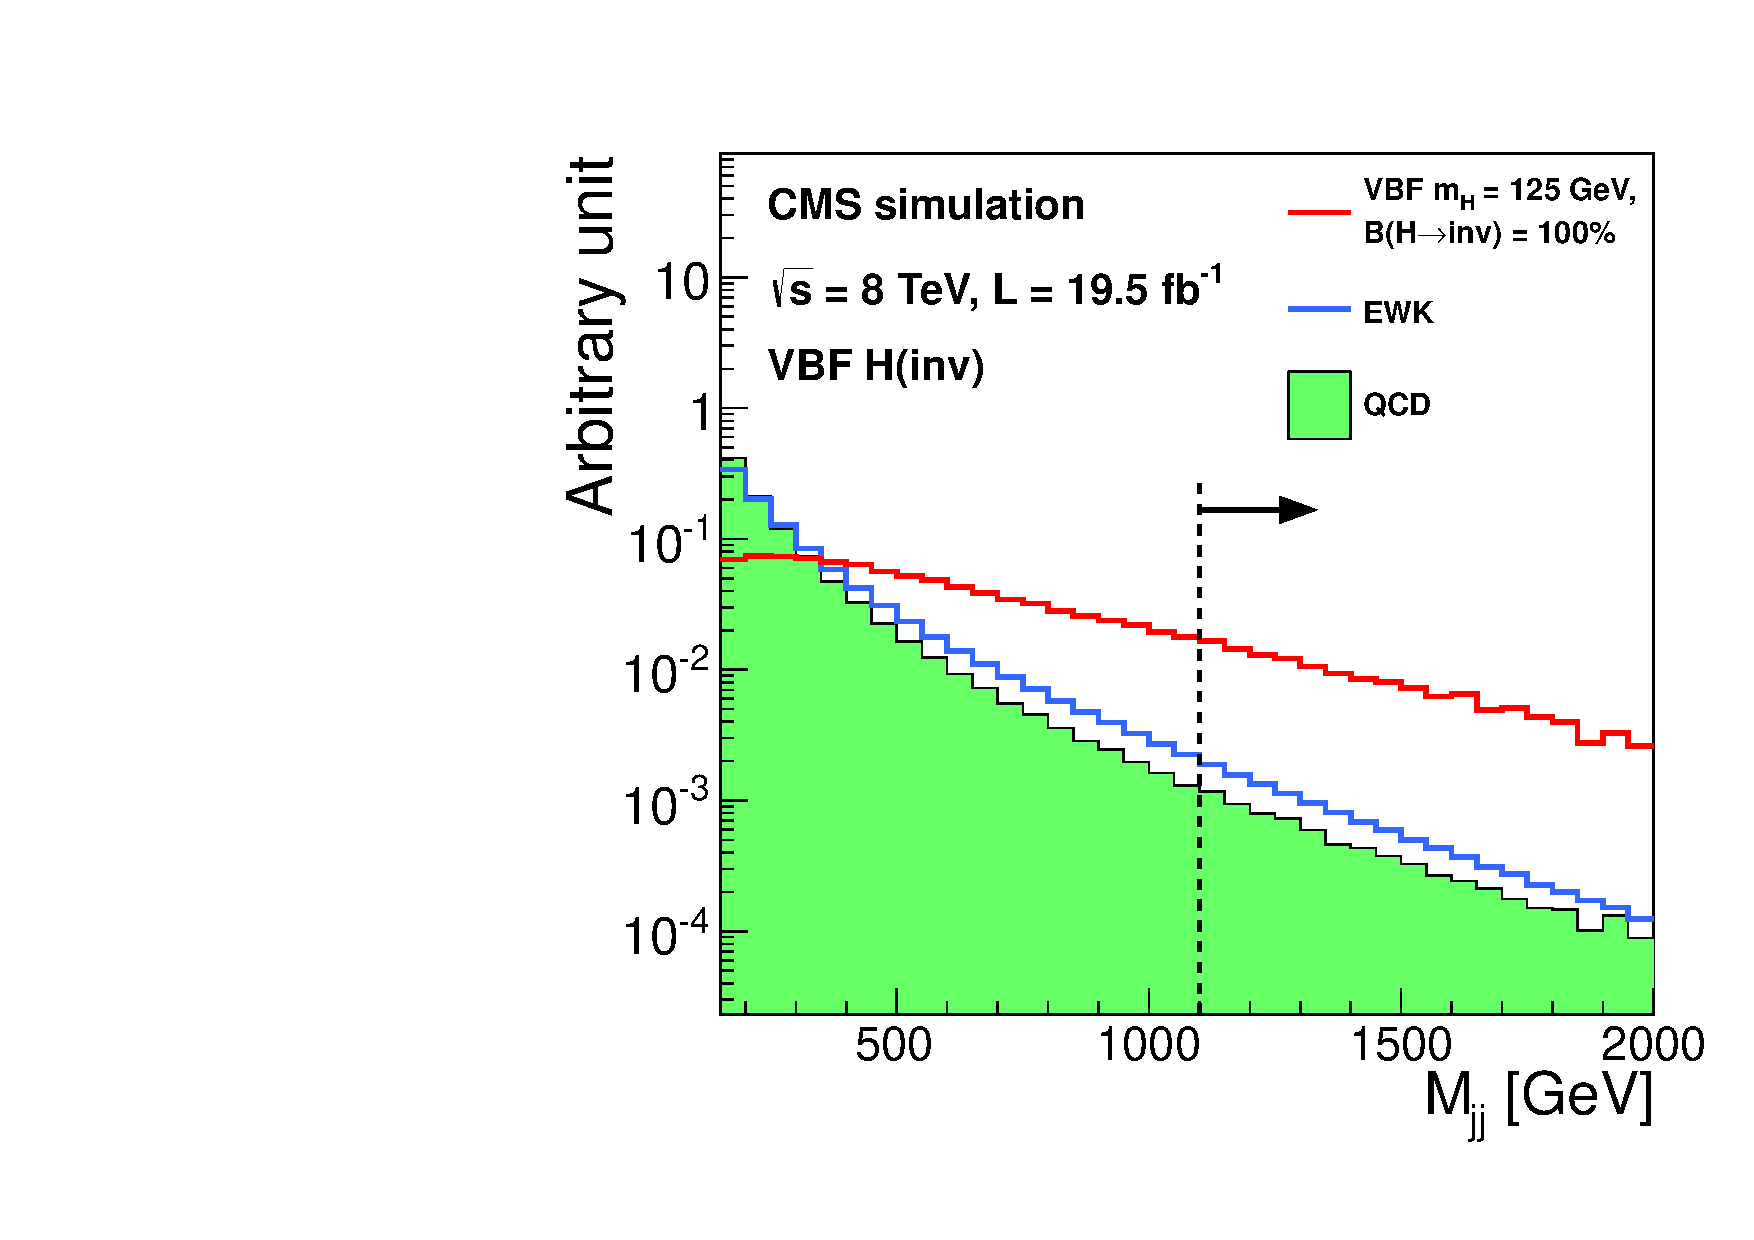
\includegraphics[width=0.49\textwidth]{Chapter05/Images/VBF-Dijet-M.pdf}
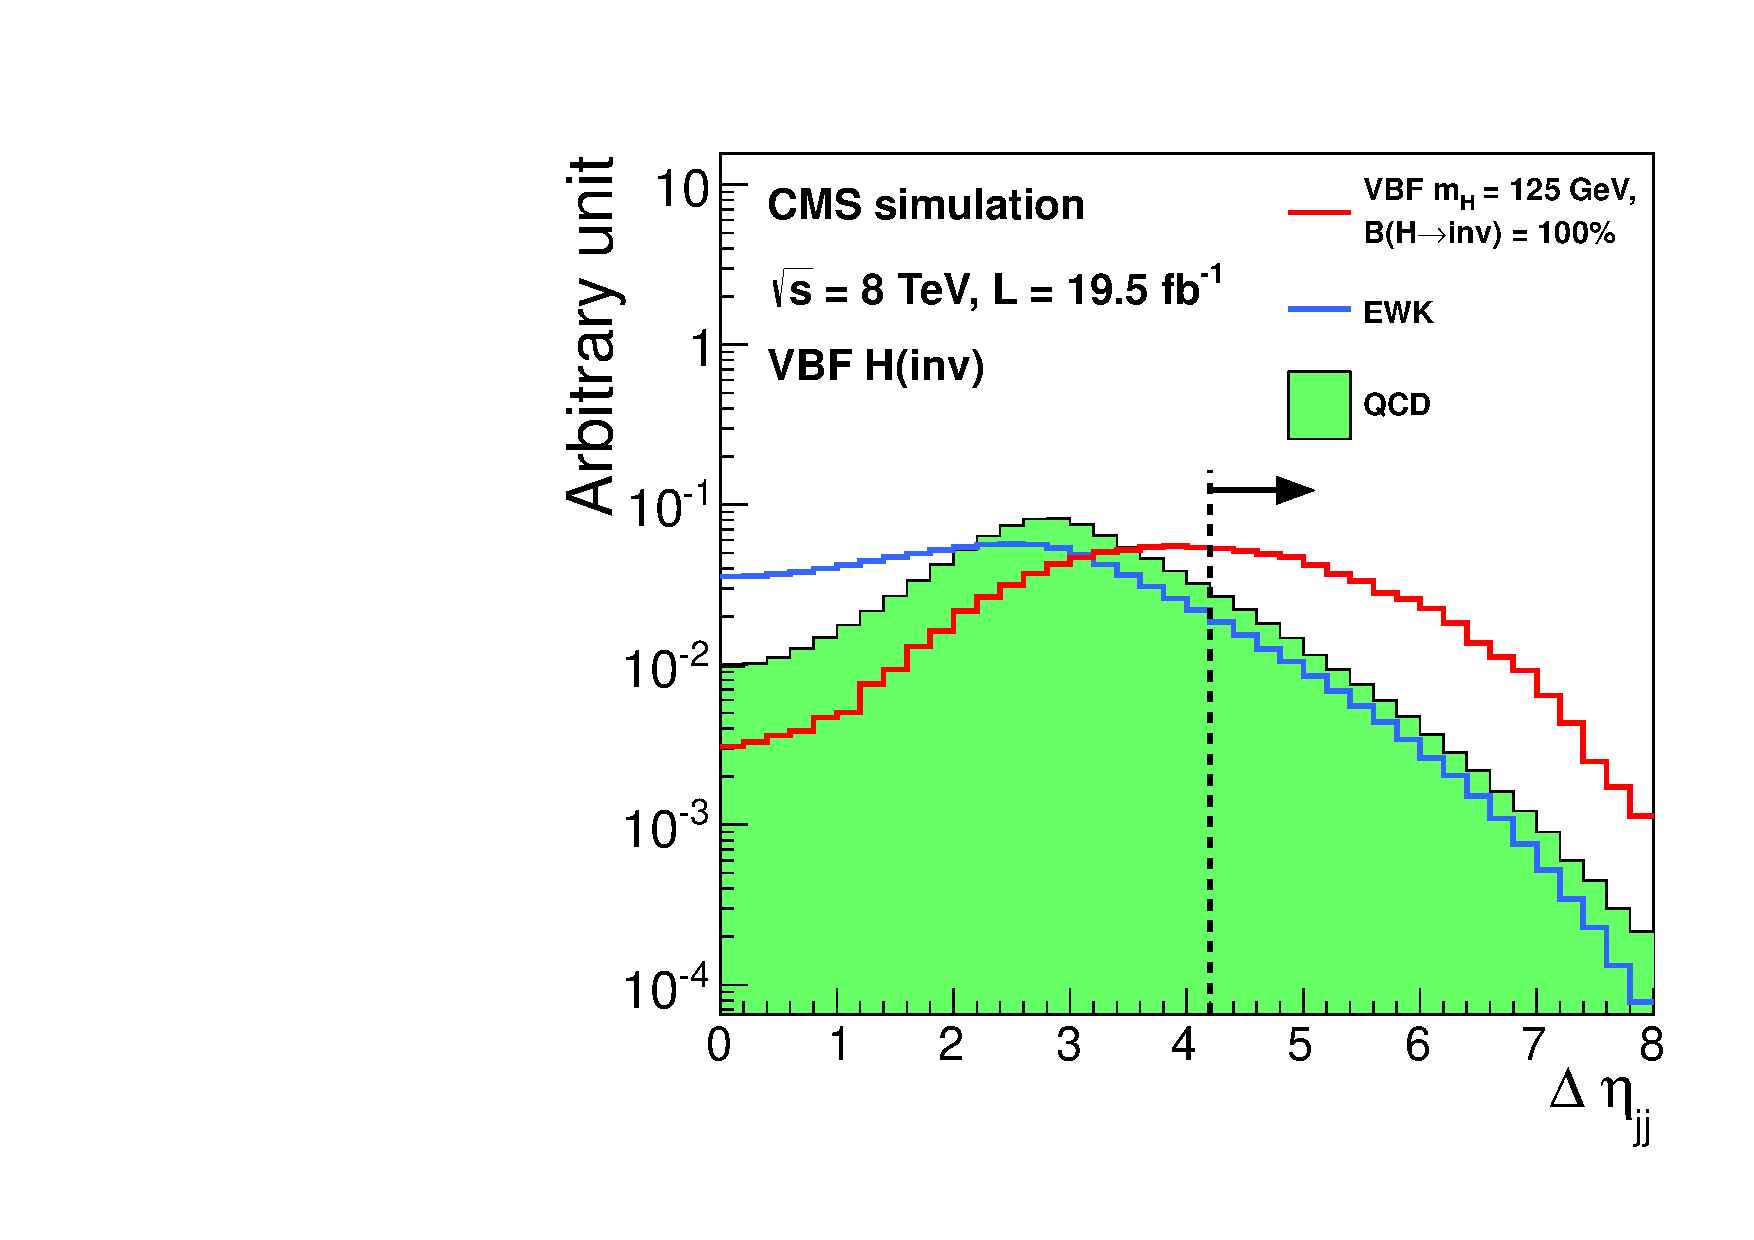
\includegraphics[width=0.49\textwidth]{Chapter05/Images/VBF-Dijet-DEta.pdf}     
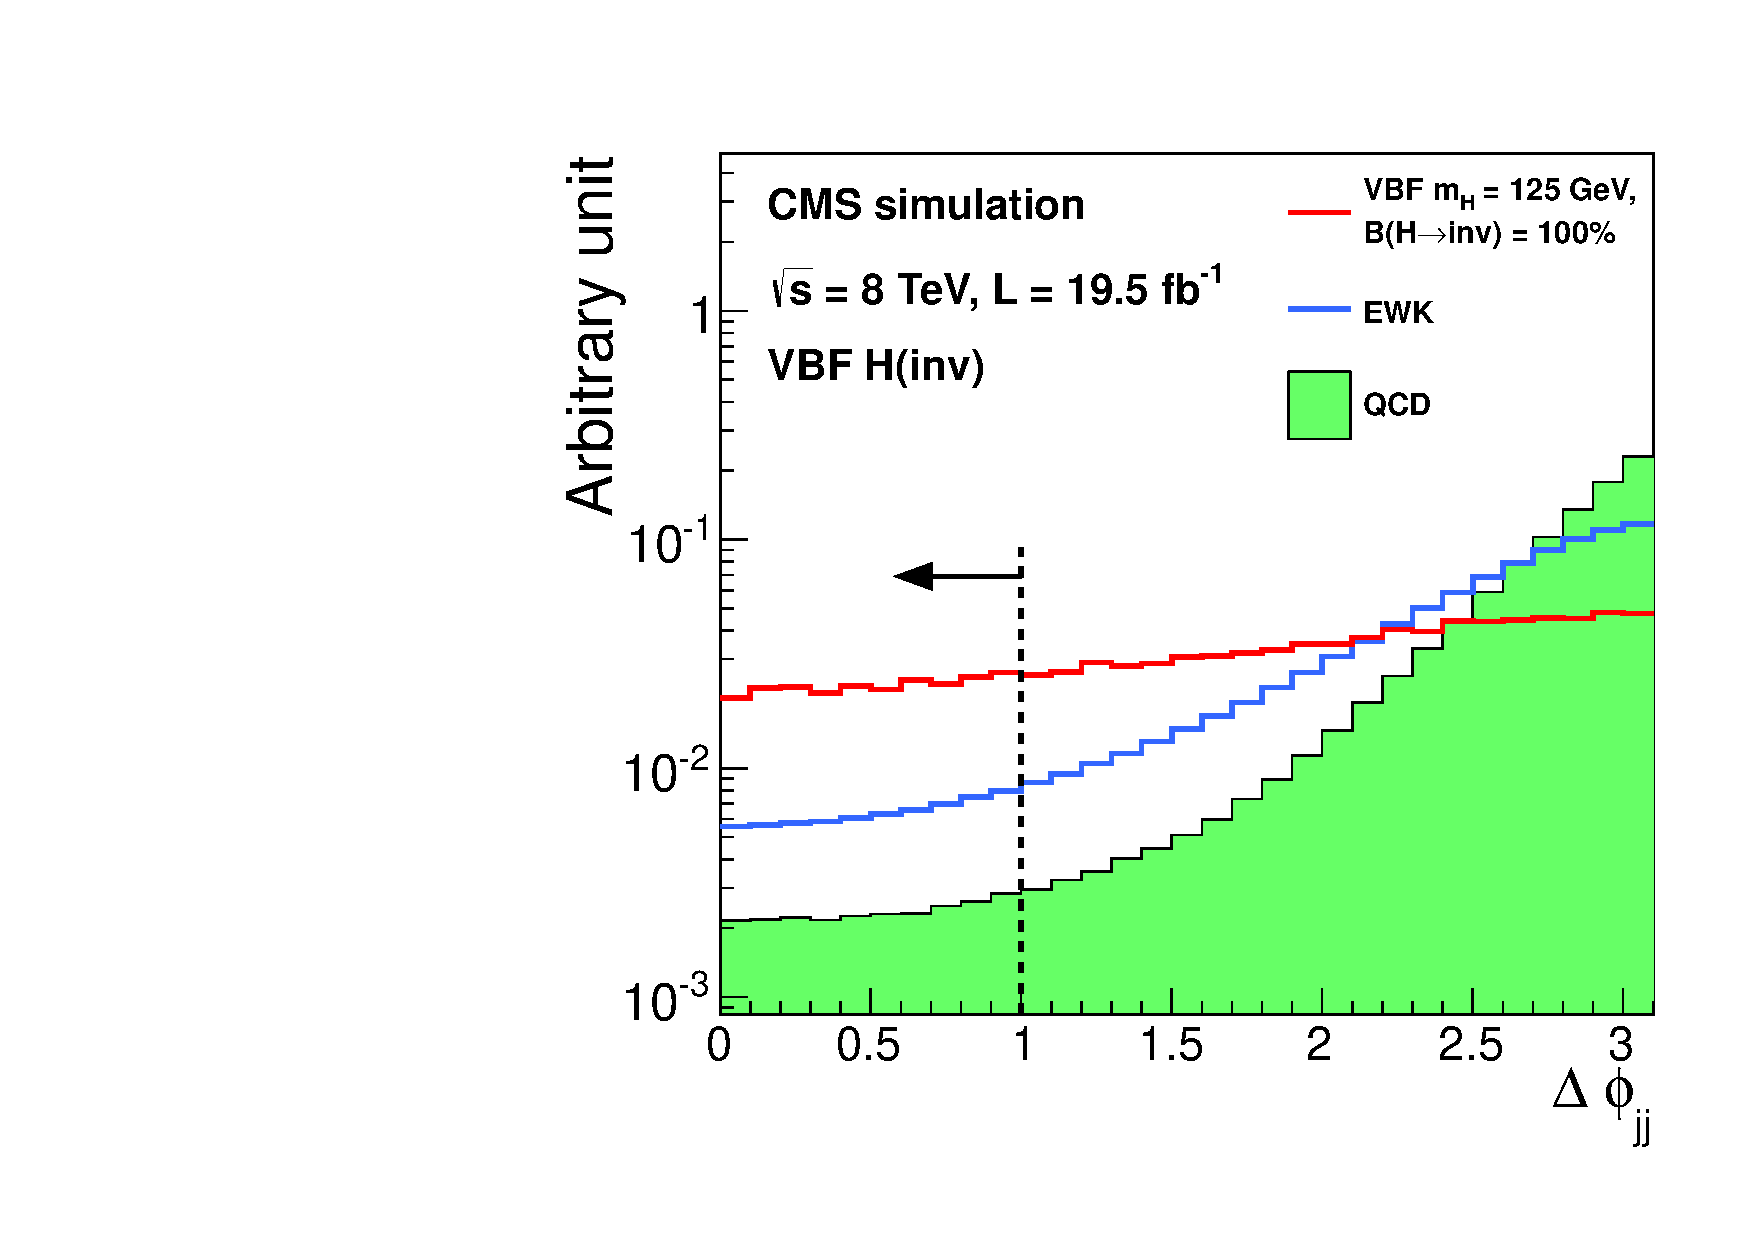
\includegraphics[width=0.49\textwidth]{Chapter05/Images/VBF-Dijet-DPhi.pdf}
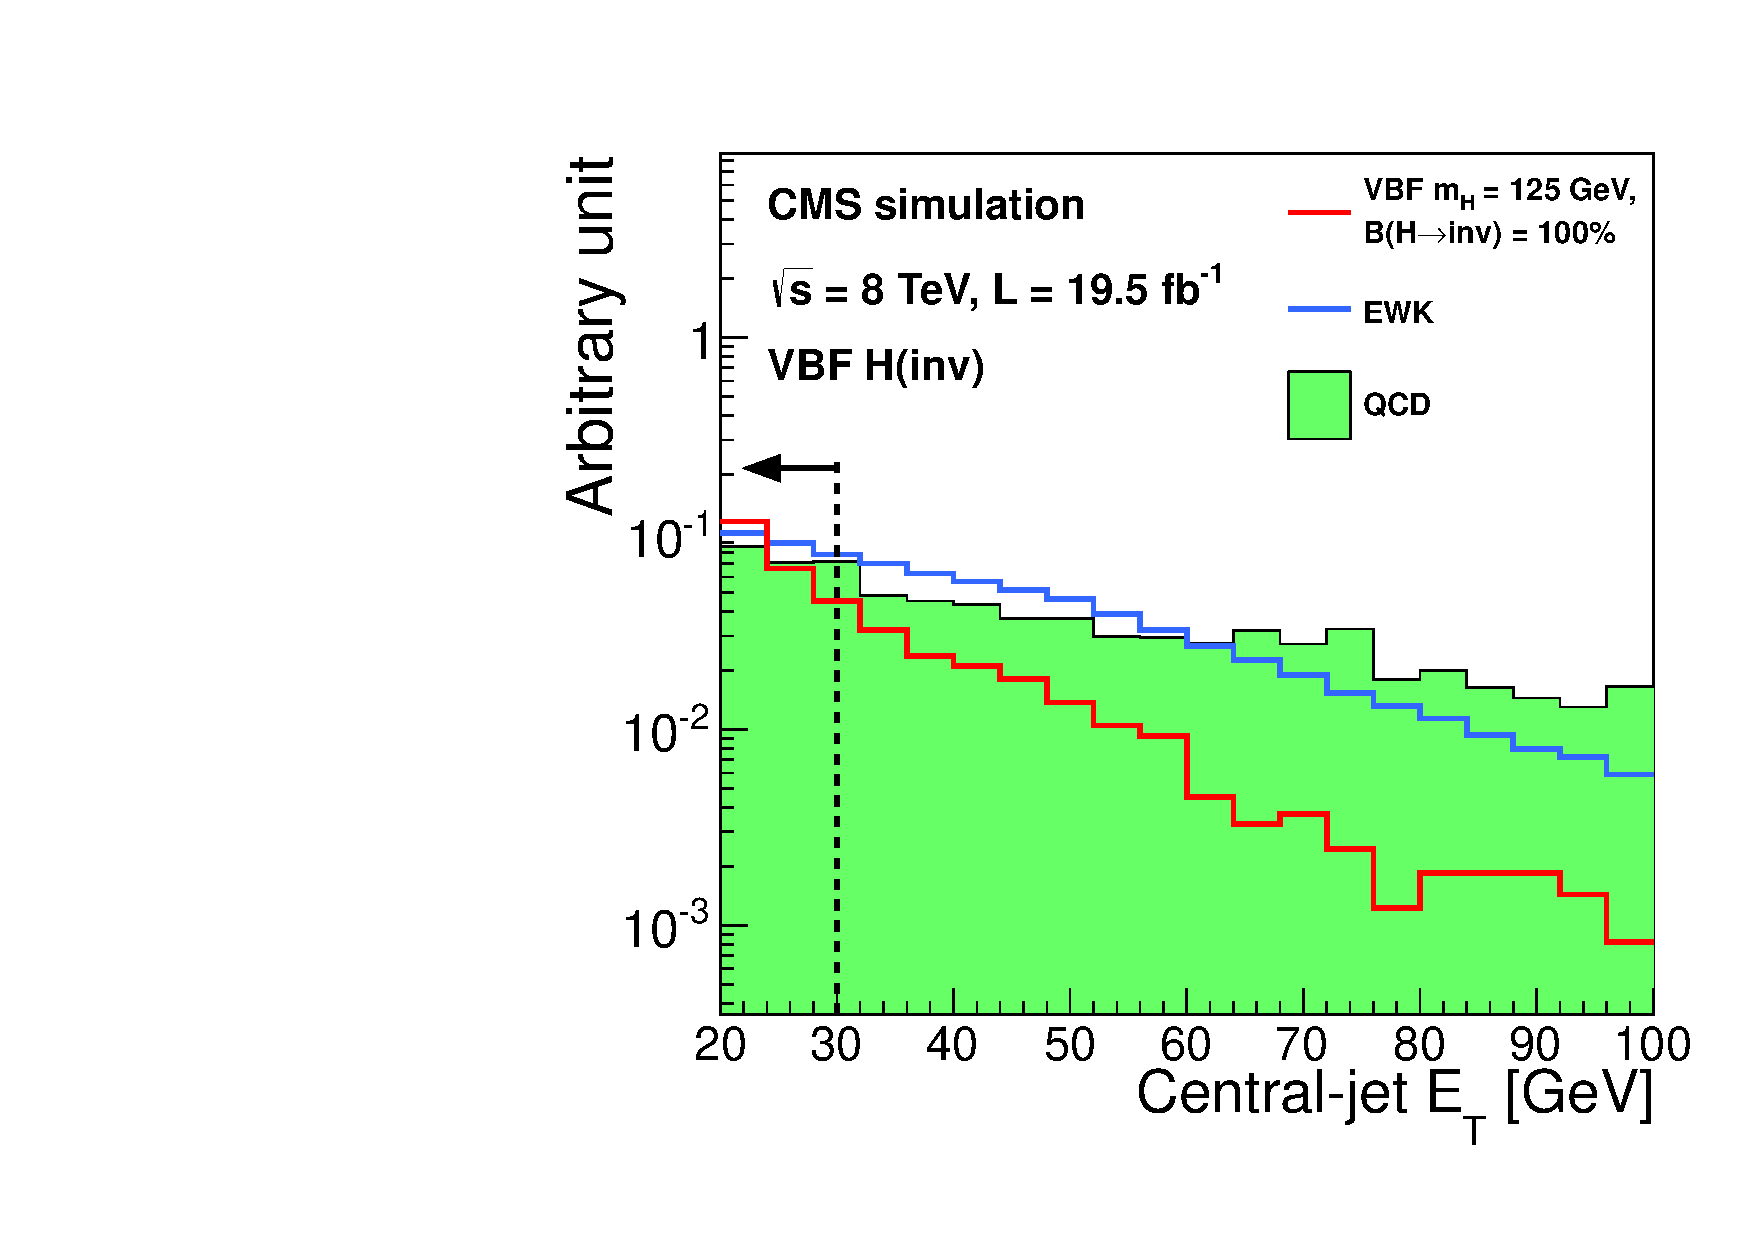
\includegraphics[width=0.49\textwidth]{Chapter05/Images/VBF-CJV-pT.pdf} 
\caption{Distributions of $M_{jj}$ (top left), $\Delta\eta_{jj}$ (top right), $\Delta\phi_{jj}$ (bottom left), and central jet \pt (bottom right) in background and signal MC simulation. The distributions are shown after requiring two jets with $\pt^{jet_1},\pt^{jet_2} > 50\,\GeV$, $|\eta| < 4.7$, $\eta_{jet1} \cdot \eta_{jet2} < 0$, $M_{jj}>150$\GeV, and $MET > 130\,\GeV$. The arrows correspond to the thresholds applied for the final selection, after optimization. \cite{ARTICLE:CMSVBFHiggsToInvAndZHCombination}}
\label{FIGURE:PromptDataAnalysis_EventSelection_KeyVariables}
\end{figure}

To estimate the signal yields the \textsc{POWHEG} \gls{MC} generator was used to create events with a Higgs boson produced via the \gls{VBF} channel with \gls{SM} couplings and with mass of $125\,\GeV$. The obtained signal efficiency was $(6.8 \pm 0.3) \times 10^{-3}$, which corresponds to an event yield of $210 \pm 29\syst$. The signal efficiency dependency on jet $\pt$, dijet $M_jj$, and \gls{MET} is correlated and of comparable amounts. Additionally, a small amount of gluon-fusion signal, where \gls{ISR} take the role of the \gls{VBF} jets, is also expected to pass the signal event selection. Using the same \gls{MC} event generator this contribution has been estimated to be of $14 \pm 10\syst$ events.

%%%%%%%%%%%%%%%%%%%%%%%%%%%%%%%%%%%%%%%%%%%%%%%%%%%%%%%%%%%%%%%%%%%%%%%%%%%%%%%%%%%%
%%% SECTION
%%%%%%%%%%%%%%%%%%%%%%%%%%%%%%%%%%%%%%%%%%%%%%%%%%%%%%%%%%%%%%%%%%%%%%%%%%%%%%%%%%%%
\section{Background Estimation}

%Status: Writing

The irreducible background $\Z(\nu \nu)\text{+jets}$ is estimated from data using as proxy $\Z (\mu \mu)$ decays. A control region for the \Z background is defined with the same event selection as the signal region, with the following changes: instead of the muons veto a pair of opposite charge tight muons is required with an invariant mass compatible with a \Z decay of $60 < M_{\mu\mu}<120\,\GeV$. We veto the event if any more additional veto electrons or loose muons are present. We use $MET_{no-\mu}$ to emulate the signature from a \Z decay into neutrinos. We can extrapolate the number of events in signal region using equation \ref{EQUATION:FIGURE:PromptDataAnalysis_BackgroundEstimation_Zmumu}.

\begin{equation}
N^\mathrm{s}_{\nu\nu} = (N^\mathrm{c}_{\mu\mu\text{obs}} - N^\mathrm{c}_\text{bkg}) \cdot \frac{\sigma(\Z \to \nu\nu)}{\sigma(\Z/\gamma^{*} \to \mu\mu)} \cdot \frac{\varepsilon^\mathrm{s}_{\Z \mathrm{MC}}}{\varepsilon^\mathrm{c}_{\Z \mathrm{MC}}}.
\label{EQUATION:FIGURE:PromptDataAnalysis_BackgroundEstimation_Zmumu}
\end{equation}

%TODO: I think its DY to mumu only

The \textsc{MCFM} \gls{MC} generator \cite{ARTICLE:MCFMGenerator} was used to estimate the the ratio of cross sections in equation \ref{EQUATION:FIGURE:PromptDataAnalysis_BackgroundEstimation_Zmumu} as $\sigma(\Z \to \nu \nu) / \sigma(\Z/\gamma^{*} \to \mu \mu) = 5.651 \pm 0.023\syst$ for $m_{\Z/\gamma^{*}} > 50\,\GeV$. The selection efficiency terms are calculated using a DY($\ell\ell$)+jets \gls{MC} simulation, for the signal region the muons are ignored and the obtained efficiency is $\varepsilon^\mathrm{s}_{\Z \mathrm{MC}} = (1.65 \pm 0.27\syst)$ and $\varepsilon^\mathrm{c}_{\Z \mathrm{MC}}=(1.11 \pm 0.17\syst) \times 10^{-6}$ for the control region. The event yield observed in this control region is of $N^\mathrm{c}_{\mu\mu\text{obs}} = 12$ events. The other backgrounds in the control region are estimated using \gls{MC} simulation of the $\ttbar$, diboson and single-top processes being $N^\mathrm{c}_\text{bkg}=0.23 \pm 0.15\syst$ event. Using  these results the contribution of the  $\Z (\nu \nu)$ background in the signal region is estimated as $99 \pm 29\stat \pm 25\syst$ events. Figure \ref{FIGURE:PromptDataAnalysis_BackgroundEstimation_ZControlRegion} shows the \gls{MET} and dijet invariant mass distributions with a less strict \Z control region event selection, where $\Delta\eta_{jj}$, $\Delta\phi_{jj}$ and \gls{CJV} requirements are not enforced and we require dijet $M_{jj}>1000\,\GeV$. 

\begin{figure}[!htb]
\centering
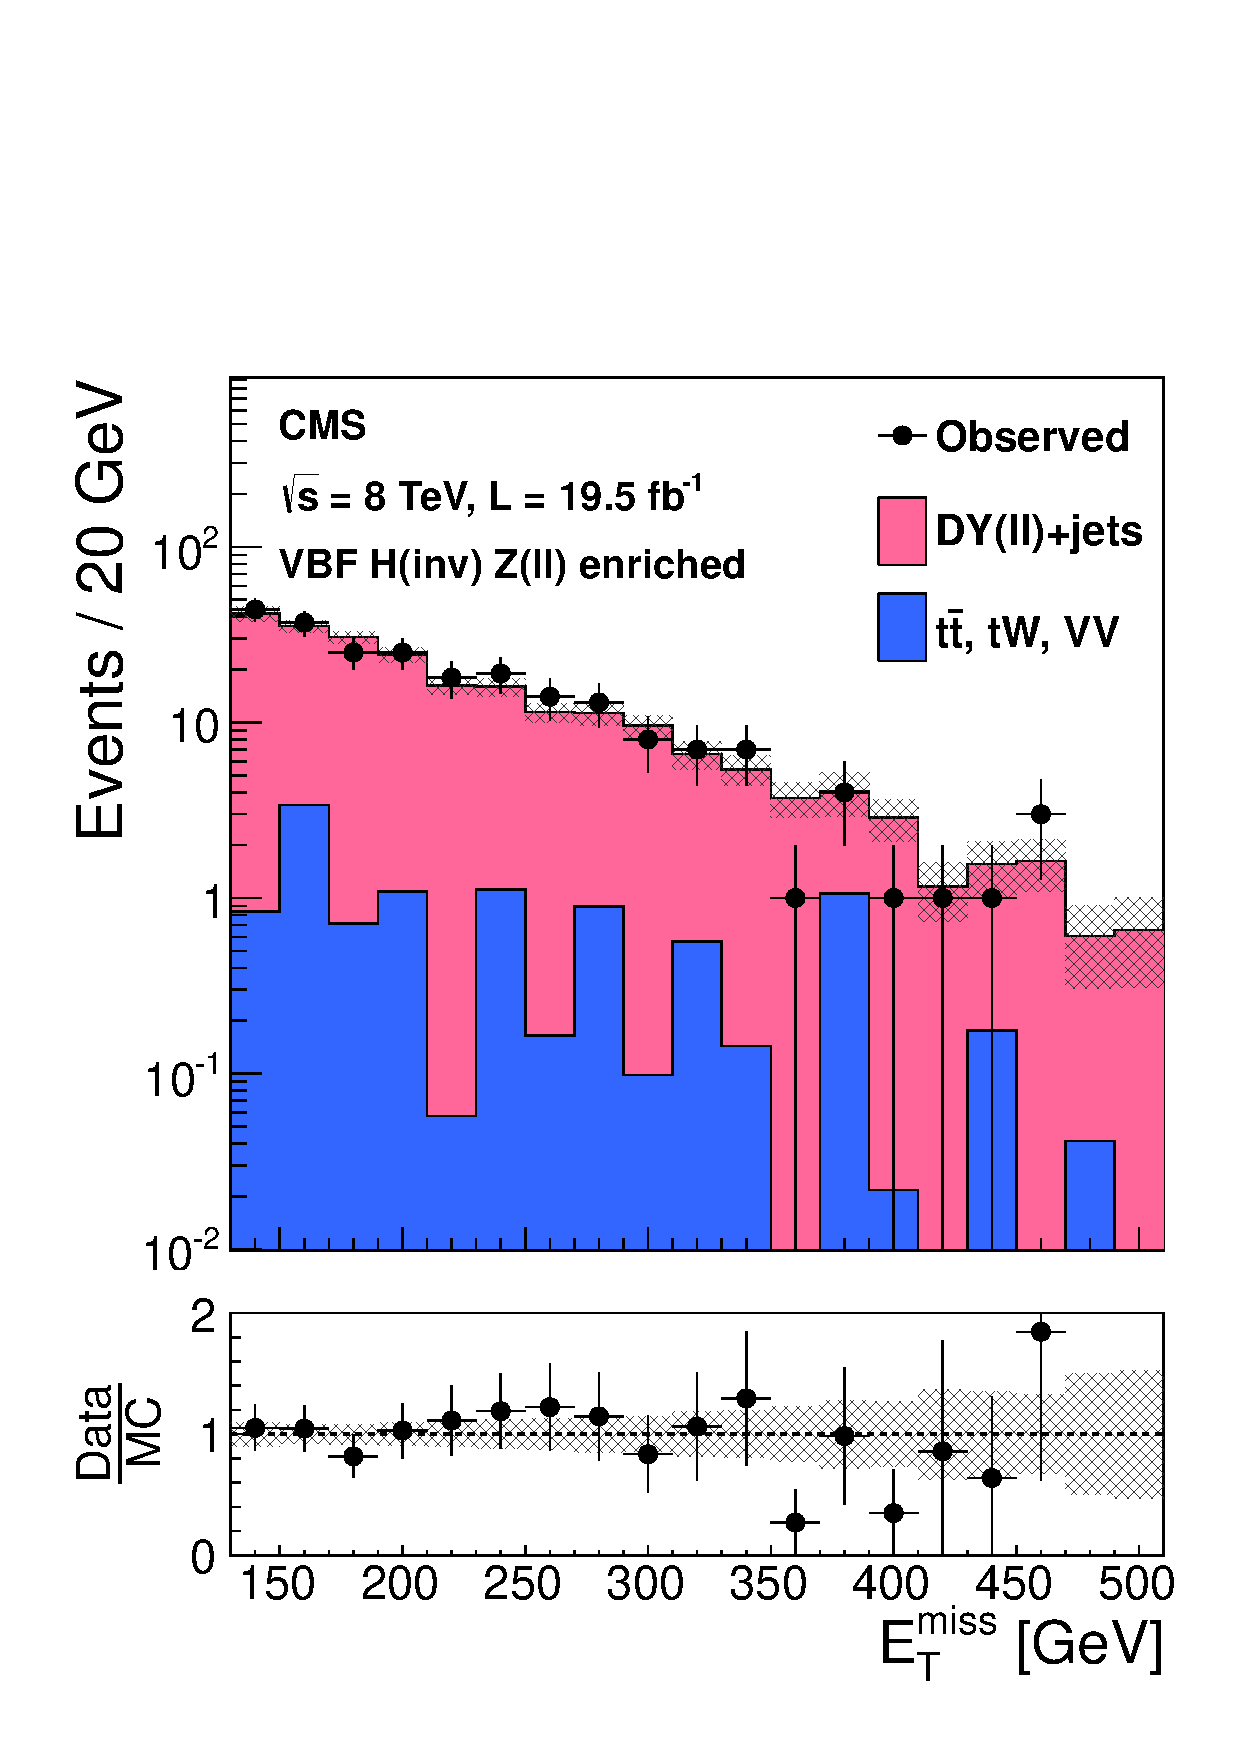
\includegraphics[width=0.45\textwidth]{Chapter05/Images/ZCtrlMET.pdf}
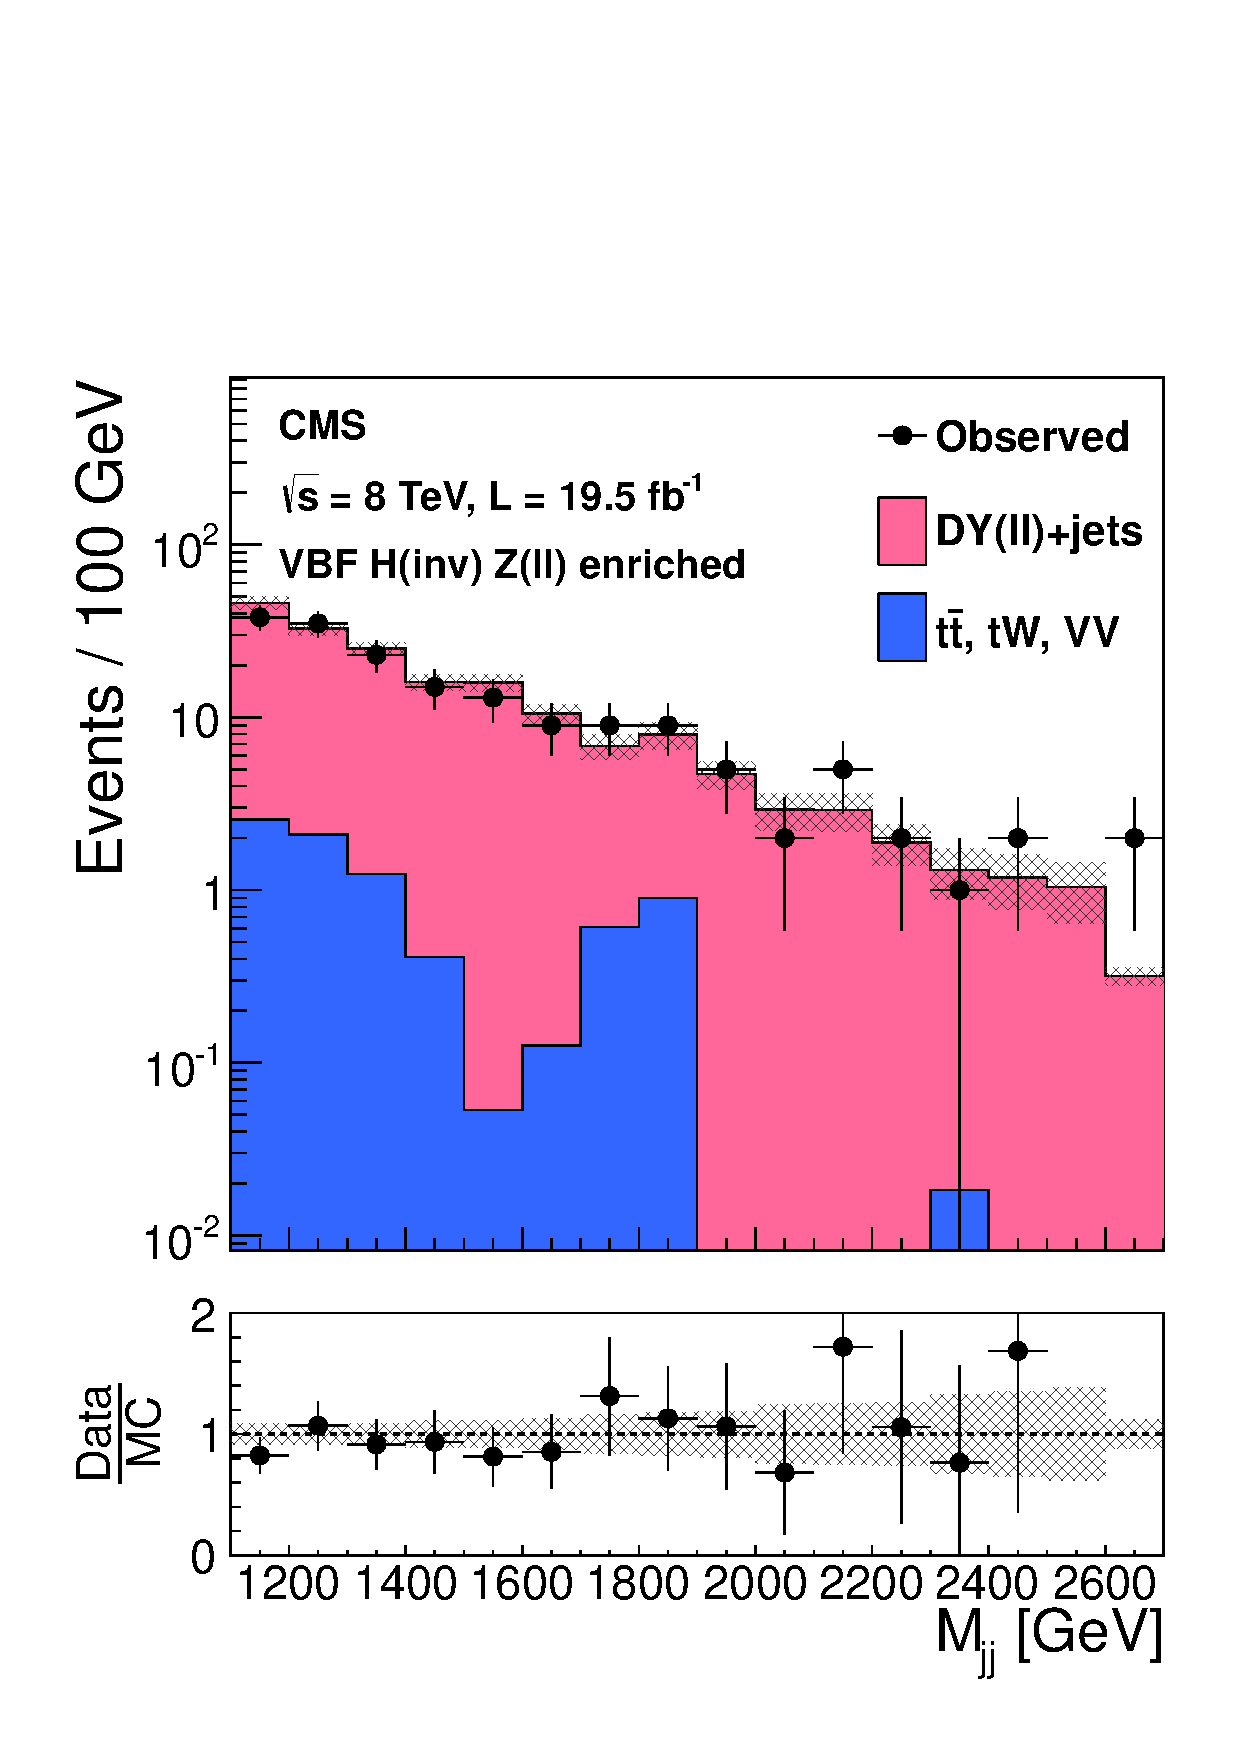
\includegraphics[width=0.45\textwidth]{Chapter05/Images/ZCtrlMjj.pdf}   
\caption{Distribution for \gls{MET} on the right and $M_{jj}$ on the left for a relaxed $Z$ control region, with no requirements on $\Delta\eta_{jj}$, $\Delta\phi_{jj}$, or \gls{CJV} and with a $M_{jj}>1000\,\GeV$ requirement. Backgrounds are shown cumulatively, normalized to data, and with systematic uncertainty shown as a hatched region. The lower panels show the ratio of data to the simulated background. \cite{ARTICLE:CMSVBFHiggsToInvAndZHCombination}}
\label{FIGURE:PromptDataAnalysis_BackgroundEstimation_ZControlRegion}
\end{figure}

The W boson backgrounds, $\PW (\Pe \nu)\text{+jets}$ and $\PW (\mu \nu)\text{+jets}$, are estimated in control region that select a single lepton. Two regions are defined following the approach used for the \Z boson background. The $\PW (\mu \nu)$ control region is defined by replacing the \textit{loose muon} veto by a requirement of one \textit{tight muon} and vetoing any event with additional \textit{loose muons}. For this control region the \gls{MET} is recomputed to not include the muons. The $\PW (\Pe \nu)$ control region is defined by replacing the \textit{veto electron} veto by a requirement of one \textit{tight electron} and vetoing any event with additional \textit{veto electrons}. For this control region we do not recompute \gls{MET} since it is include in the trigger requirements. Equation \ref{EQUATION:PromptDataAnalysis_BackgroundEstimation_WLep} can be used to extrapolate the events in both this control regions to the signal region.

\begin{equation}
N^\mathrm{s}_\ell = (N^\mathrm{c}_{\ell\text{obs}} - N^\mathrm{c}_\text{bkg}) \cdot \frac{N^\mathrm{s}_{\PW \mathrm{MC}}}{N^\mathrm{c}_{\PW \mathrm{MC}}},
\label{EQUATION:PromptDataAnalysis_BackgroundEstimation_WLep}
\end{equation}

Where $N^\mathrm{s}_{\PW \mathrm{MC}}$ and $N^\mathrm{c}_{\PW \mathrm{MC}}$  are the number of event in signal and control regions $\PW (\ell \nu)\text{+jets}$ obtained from \gls{MC} simulation. These rations are estimated as $N^\mathrm{s}_{\PW \mathrm{MC}}/N^\mathrm{c}_{\PW \mathrm{MC}}$ is equal to $0.347 \pm 0.045\syst$ for $\PW (\mu \nu)$ and $1.08 \pm 0.21\syst$ for $\PW (\Pe \nu)$. In data the observed yields is the $\PW (\mu \nu)$ control region is 223 events, with estimated backgrounds from other processes of $30.4 \pm 7.0\syst$ events. For the $\PW (\Pe \nu)$ control region the observed yield is 65 events with estimated backgrounds from other processes of $7.1 \pm 4.7\syst$ events. The  extrapolated background in the signal region is $66.8 \pm 5.2\stat \pm 15.7\syst$ events for the $\PW (\mu \nu)$ background and  $62.7 \pm 8.7\stat \pm 18.1\syst$ for the $\PW (\Pe \nu)$ background.

The $\PW (\tau \nu)\text{+jets}$ process where the tau decays hadronically $\tau_{had}$ needs to be estimated differently, since there is no tau veto in the signal selection. The $\PW (\tau_{had} \nu)$ control region is defined like the signal region with the additional requirement of one tau following the description of chapter \ref{CHAPTER:EventReconstructionAndSimulation}, no other additional lepton are allowed, and the \gls{CJV} is not applied to increase the yield. We estimated the yield in the signal region $N^\mathrm{s}_{\tau_{had}}$ using equation \ref{EQUATION:PromptDataAnalysis_BackgroundEstimation_WTau}. A conversion factor is derived by dividing the efficiency of the \gls{CJV} in this selection by the efficiency of the $\PW (\tau_{had} \nu)$ control region including the \gls{CJV} over the $\PW (\tau_{had} \nu)$ process events sample, both determined from \gls{MC} simulation. The efficiency of the tau control region selection with the \gls{CJV} was estimated as $\varepsilon_{\tau}$ is $0.134 \pm 0.023\syst$. 

\begin{equation}
N^\mathrm{s}_{\tau_{had}} = (N^\mathrm{c}_{\tau\text{obs}} - N^\mathrm{c}_\text{bkg}) \cdot \frac{\varepsilon_\mathrm{CJV}}{\varepsilon_{\tau}},
\label{EQUATION:PromptDataAnalysis_BackgroundEstimation_WTau}
\end{equation}
 
In this control region a yield of $15.2 \pm 3.6\syst$ events was observed, leading to an estimated signal region contribution for the $\PW (\tau_{had} \nu)$ background of $53 \pm 18\stat \pm 18\syst$ events.

To increase the confidence in the \gls{MC} background model and the extrapolations to the signal regions, we compute the expected data yields from one control regions to another using conversion factors determined from \gls{MC} simulation. For example, the $\PW (\mu \nu)$ control region date yield is used to compute yieldof the the $\Z (\mu \mu)$ region is given by using equation \ref{EQUATION:PromptDataAnalysis_BackgroundEstimation_RegionCrossCheck}. In all cases, the estimations agreed, within uncertainties, with the observed yields in data. 

\begin{equation}
N^\mathrm{c}_{\mu \mu} = (N^\mathrm{c}_{\mu \text{obs}} - N^\mathrm{c}_\text{bkg}) \cdot \frac{N^\mathrm{c}_{\Z \mathrm{MC}}}{N^\mathrm{c}_{\PW \mathrm{MC}}},
\label{EQUATION:PromptDataAnalysis_BackgroundEstimation_RegionCrossCheck}
\end{equation}


% The QCD multijet background in the signal region is estimated using the fractions of events passing the $\ETm$ and CJV requirements.  We define regions A, B, C, and D as follows, after the full remaining selection :
% 
% \begin{itemize}
%         \item{A: fail $\ETm$ selection, fail CJV selection;}
%         \item{B: pass $\ETm$ selection, fail CJV selection;}
%         \item{C: fail $\ETm$ selection, pass CJV selection;}
%         \item{D: pass $\ETm$ selection, pass CJV selection.}
% \end{itemize}
% 
% We estimate the QCD multijet component in regions A, B, and C from data, after subtracting the electroweak backgrounds using estimations from simulation.  The QCD multijet component in the signal region D can then be estimated using $N_\mathrm{D} = N_\mathrm{ B}N_\mathrm{C} / N_\mathrm{A}$, where $N_{i}$ is the number of events in region $i$.  This method is based on the assumption that the $\ETm$ and the CJV are uncorrelated, which has been checked by comparing the $\ETm$ distribution, below the 130\GeV threshold, in events passing and failing the CJV.  The maximum difference in the $\ETm$ distribution between these two samples is 40\%, which is assigned as a systematic uncertainty of the method.  We predict the QCD background in the signal region to be $30.9 \pm 4.8\stat \pm 23.0\syst$ events.  Furthermore, the method is tested on a high statistics sample with selections equivalent to those in the signal region, but dominated by QCD multijet events by changing the $\phijj$ requirement to $\phijj>2.6$~radians.  In this sample, we observe $2551 \pm 57\stat$ events in the pseudo-signal region after subtraction of backgrounds, which are estimated from MC simulation.  The QCD multijet component is predicted to be $2959 \pm 58\stat$, which is compatible with the observation within the systematic uncertainty.  To give further confidence in this estimate, we perform a cross-check using an ABCD method based on the $\ETm$ and $\phijj$ variables, which gives a prediction consistent with the main method.
% 
% The remaining SM backgrounds in the signal region---due to $\ttbar$, single-top, VV and DY($\ell\ell$)+jets---are estimated from MC simulation to be $20.0 ^{+6.0}_{-8.2}\syst$ events.  The total expected background is $332 \pm 36\stat \pm 45\syst$.  The background estimates are summarised in Table~\ref{tab:bgSummary} along with the expected yield for a signal with $\mH=125$\GeV and $\BRinv=100$\%.

\begin{table}[!htb]
\centering
\begin{tabular}{|l|c|}
\hline
Process                                  & Event yields                  \\
\hline
$\Z (\nu\nu)\text{+jets}$                & $  99 \pm  29 \stat \pm 25 \syst$  \\
$\PW (\mu\nu)\text{+jets}$               & $  67 \pm   5 \stat \pm 16 \syst$   \\
$\PW (\Pe \nu)\text{+jets}$              & $  63 \pm   9 \stat \pm 18 \syst$   \\
$\PW (\tau_{haf} \nu)\text{+jets}$       & $  53 \pm  18 \stat \pm 18 \syst$  \\
QCD multijet                             & $  31 \pm   5 \stat \pm 23 \syst$   \\
Sum (\ttbar, single top quark, $VV$, DY) & $20.0 \pm 8.2 \syst$ \\
\hline\hline
Total background                         & $332 \pm 36 \stat \pm 45 \syst$ \\
VBF H(inv.)                              & $210 \pm 29 \syst$ \\
ggF H(inv.)                              & $ 14 \pm 10 \syst$ \\
Observed data                            & 390  \\
\hline\hline
S/B                                      & 70\% \\
\hline
\end{tabular}
\label{tab:bgSummary}
\caption{Summary of the estimated number of background and signal events, together with the observed yield, in the \gls{VBF} search signal region.  The signal yield is given for $m_H=125$\GeV and $\BRinv=100$\%. \cite{ARTICLE:CMSVBFHiggsToInvAndZHCombination}}
\end{table}

%%%%%%%%%%%%%%%%%%%%%%%%%%%%%%%%%%%%%%%%%%%%%%%%%%%%%%%%%%%%%%%%%%%%%%%%%%%%%%%%%%%%
%%% SECTION
%%%%%%%%%%%%%%%%%%%%%%%%%%%%%%%%%%%%%%%%%%%%%%%%%%%%%%%%%%%%%%%%%%%%%%%%%%%%%%%%%%%%
\section{Sources of uncertainty}

%Status: Writing

\begin{table}[!htb]
\centering
\begin{tabular}{|l|c|c|}
\hline
Source                                           & Total background & Signal \\
\hline\hline
Control region statistics                        & 11\%             & -      \\
MC statistics                                    & 11\%             & 4\%    \\
Jet/$E_T^{\text{miss}}$ energy scale/resolution  & 7\%              & 13\%   \\
QCD background estimation                        & 4\%              & -      \\
Lepton efficiency                                & 2\%              & -      \\
Tau ID efficiency                                & 1\%              & -      \\
Luminosity                                       & 0.2\%            & 2.6\%  \\
Cross sections                                   & 0.5--1\%         & -      \\
PDFs                                             & -                & 5\%    \\
Factorization/renormalization scale              & -                & 4\%    \\
Gluon fusion signal modelling                    & -                & 4\%    \\
\hline\hline
Total                                            & 18\%             & 14\%   \\
\hline 
\end{tabular}
\caption{Summary of the uncertainties in the total background and signal yields in the VBF channel. All uncertainties affect the normalization of the yield, and are quoted as the change in the total background or signal estimate, when each systematic effect is varied according to its uncertainties. The signal uncertainties are given for $m_H=125$\GeV and $\BRinv=100$\%. \cite{ARTICLE:CMSVBFHiggsToInvAndZHCombination}}
\label{TABLE:PromptDataAnalysis_SourcesUncertaintySummary}
\end{table}


%%%%%%%%%%%%%%%%%%%%%%%%%%%%%%%%%%%%%%%%%%%%%%%%%%%%%%%%%%%%%%%%%%%%%%%%%%%%%%%%%%%%
%%% SECTION
%%%%%%%%%%%%%%%%%%%%%%%%%%%%%%%%%%%%%%%%%%%%%%%%%%%%%%%%%%%%%%%%%%%%%%%%%%%%%%%%%%%%
\section{Results}

%Status: Writing

\begin{figure}[htp]
\centering
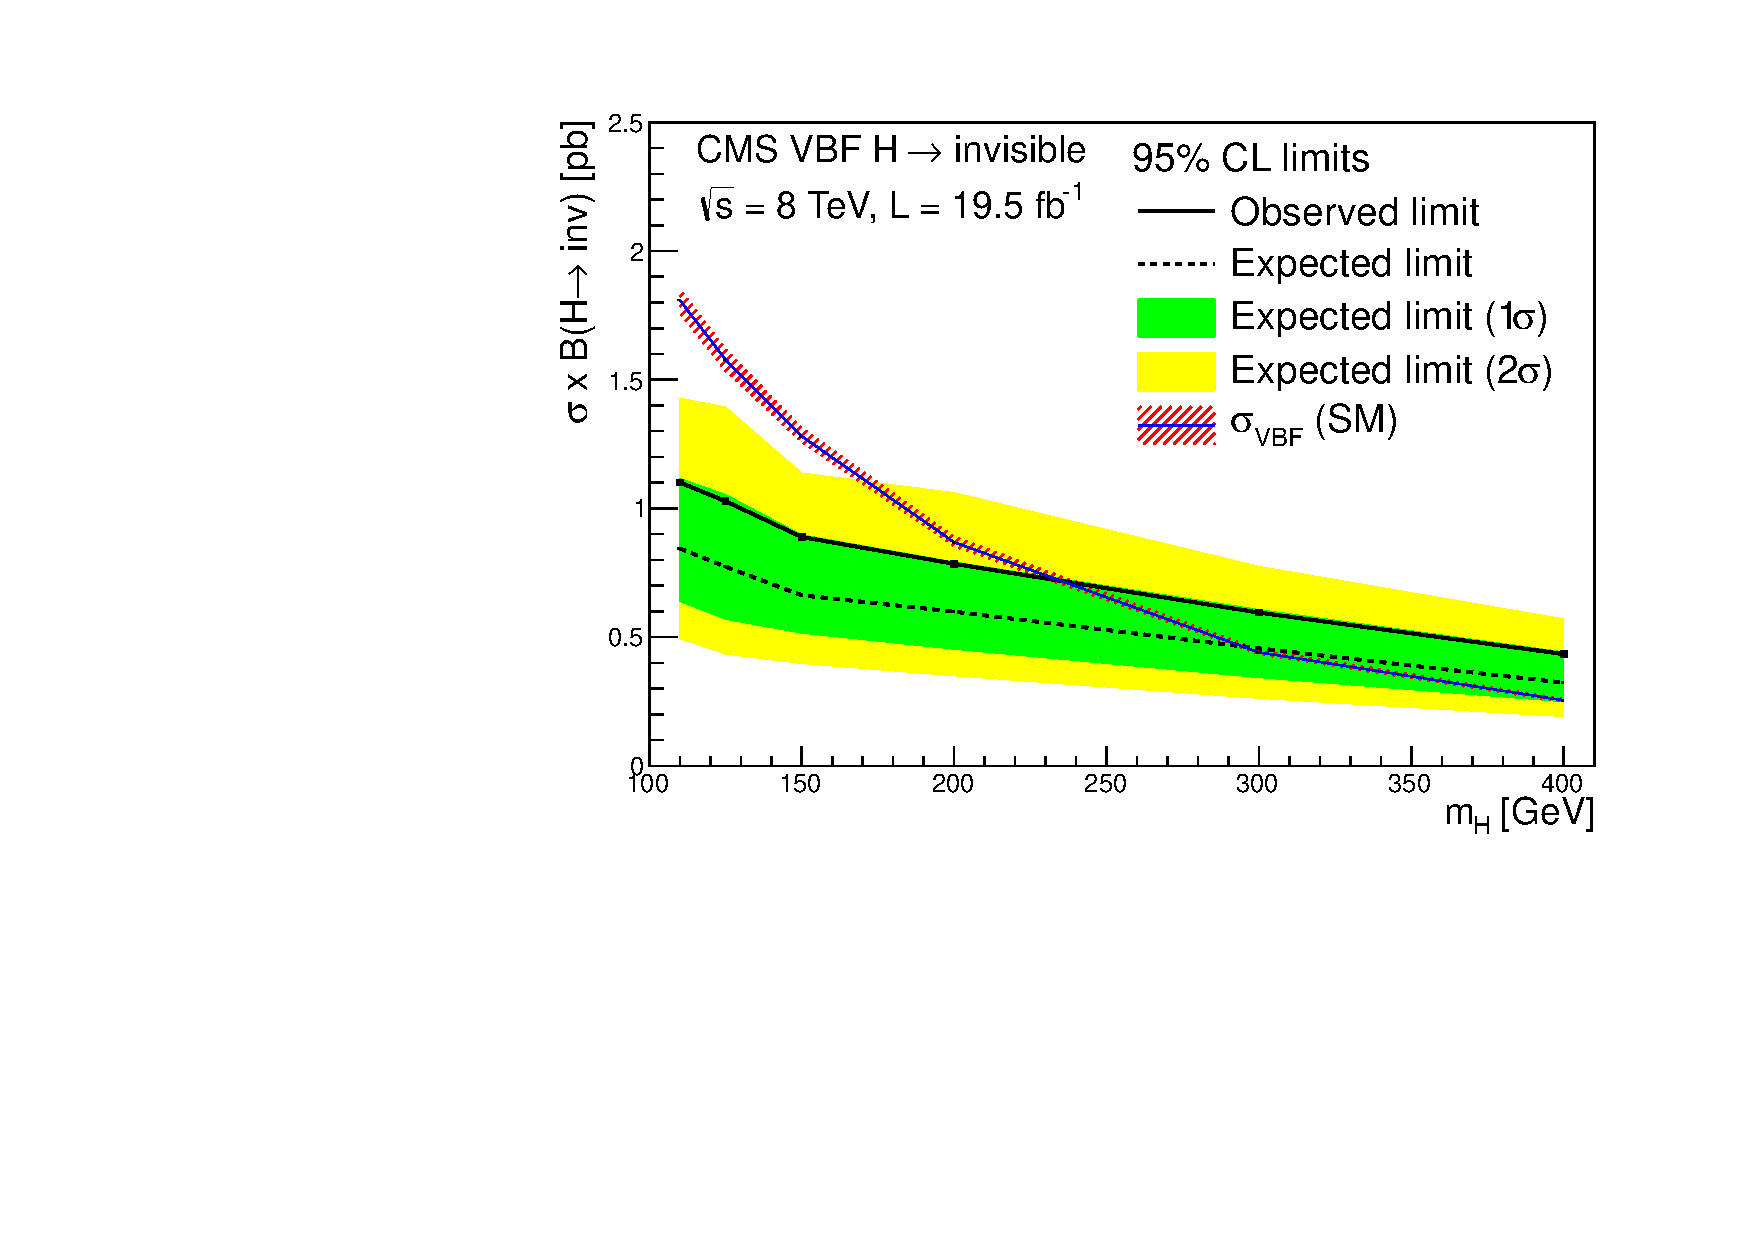
\includegraphics[width=0.49\textwidth]{Chapter05/Images/vbfxslimit.pdf}
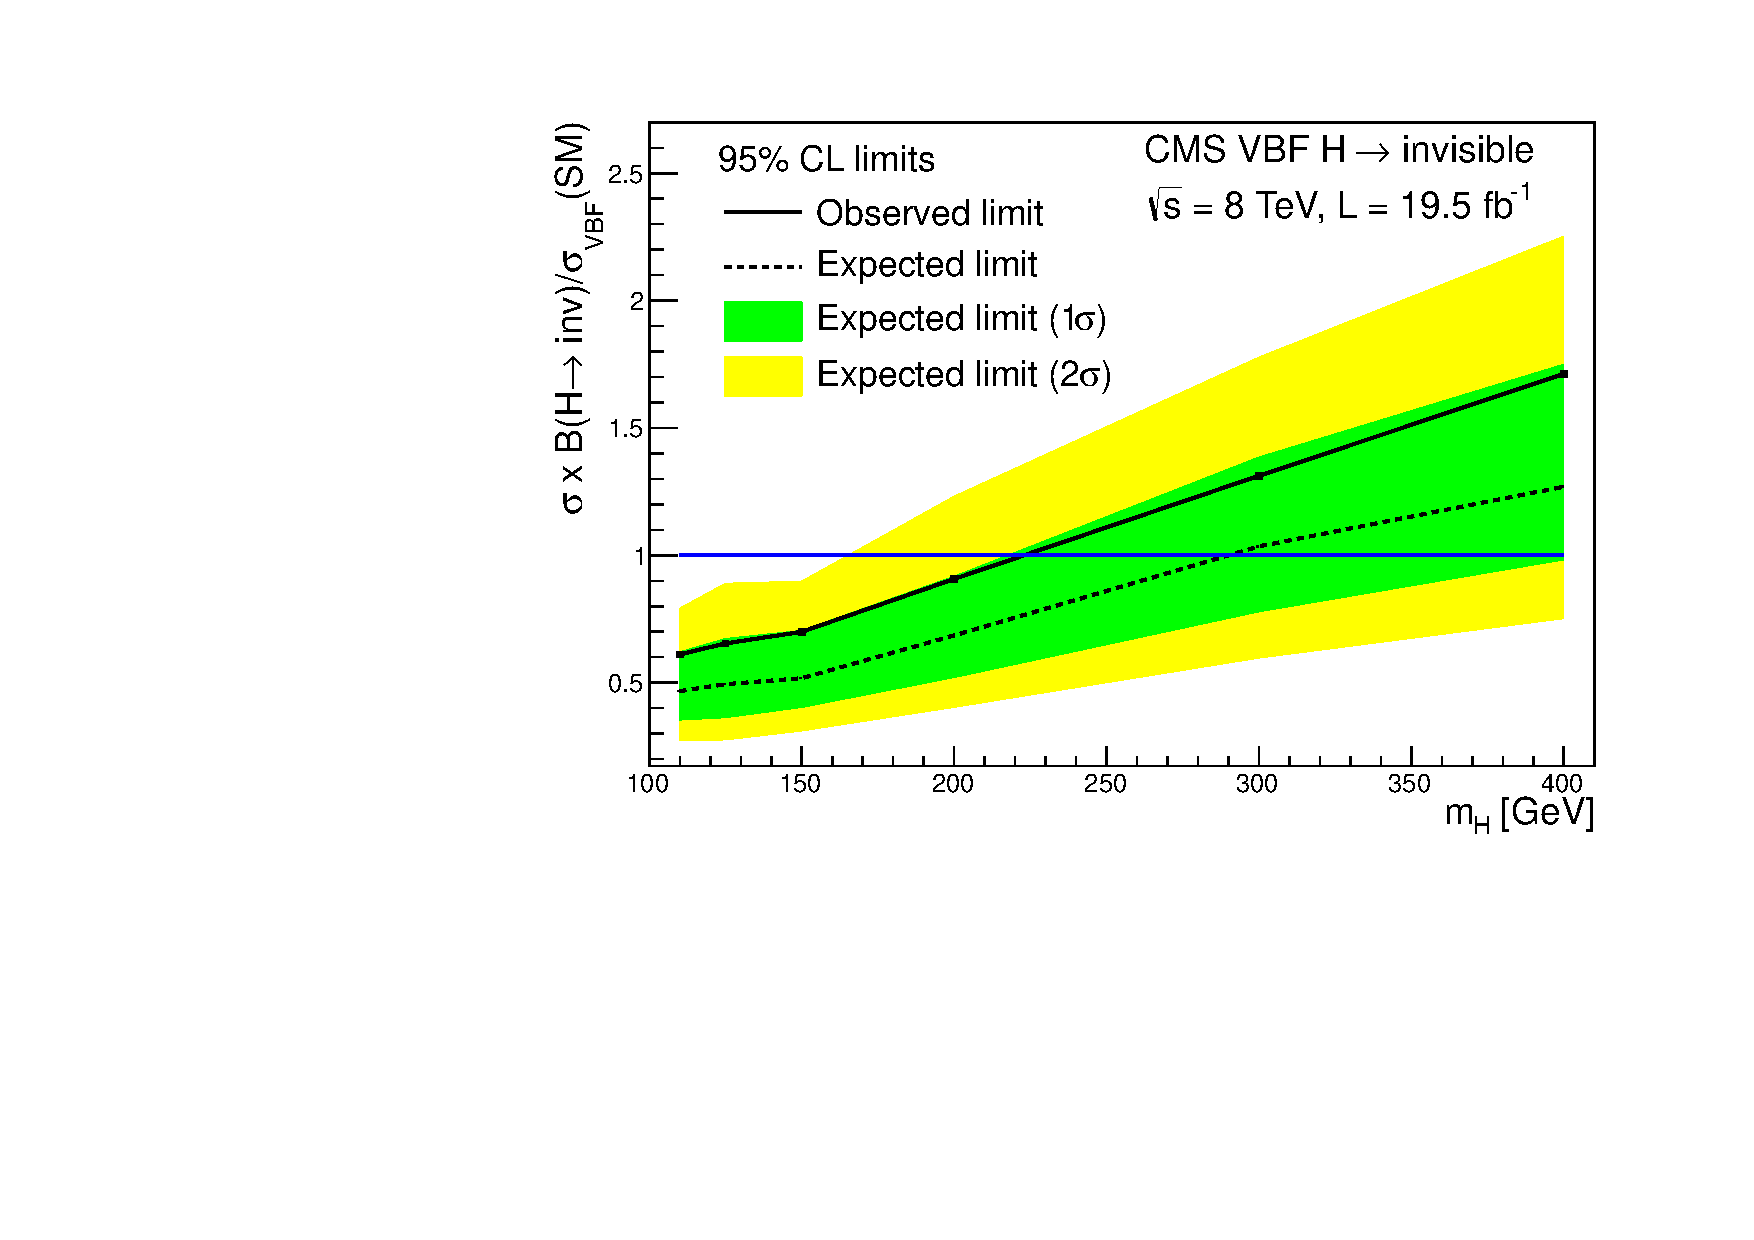
\includegraphics[width=0.49\textwidth]{Chapter05/Images/vbflimit.pdf}
\caption{Expected and observed 95\% CL upper limits on the VBF production cross section times invisible branching fraction (left figure), and normalized to the \gls{SM} Higgs boson \gls{VBF} production cross section (right figure). \cite{ARTICLE:CMSVBFHiggsToInvAndZHCombination}}
\label{FIGURE:vbfLimit}
\end{figure}


%%%%%%%%%%%%%%%%%%%%%%%%%%%%%%%%%%%%%%%%%%%%%%%%%%%%%%%%%%%%%%%%%%%%%%%%%%%%%%%%%%%%
%%% SECTION
%%%%%%%%%%%%%%%%%%%%%%%%%%%%%%%%%%%%%%%%%%%%%%%%%%%%%%%%%%%%%%%%%%%%%%%%%%%%%%%%%%%%
\section{Conclusion}

%Status: Writing


%%%%%%%%%%%%%%%%%%%%%%%%%%%%%%%%%%%%%%%%%%%%%%%%%%%%%%%%%%%%%%%%%%%%%%%%%%%%%%%%%%%%
%%% SECTION
%%%%%%%%%%%%%%%%%%%%%%%%%%%%%%%%%%%%%%%%%%%%%%%%%%%%%%%%%%%%%%%%%%%%%%%%%%%%%%%%%%%%
\section{Preparing of parked data analysis}

\subsection{Dijet-MET system topological variables}

\subsection{Track distribution variables}


%%%%%%%%%%%%%%%%%%%%%%%%%%%%%%%%%%%%%%%%%%%%%%%%%%%%%%%%%%%
% Jet topology variables
%%%%%%%%%%%%%%%%%%%%%%%%%%%%%%%%%%%%%%%%%%%%%%%%%%%%%%%%%%%
% 18 Months report was on the Sep 9 2013

%/home/hep/jca10/work/vbfinv/ws04/CMSSW_5_3_11/src/UserCode/ICHiggsTauTau/Analysis/HiggsNuNu/PLOTS_mjj1200_dijetFrac/nunu/MET130/n_vtx_2012_DijetFraction_log.pdf
% Looks like plots are from Jun 25 2013

% FOUND FILE: This is the file used in the plots for the 18 months report
%/home/hep/jca10/work/vbfinv/ws04/CMSSW_5_3_11/src/UserCode/ICHiggsTauTau/Analysis/HiggsNuNu/output_mjj1100_dijetFrac/nunu/MET130/MC_VBF_HToZZTo4Nu_M-120.root

%/vols/cms02/jca10/work/ws01/CMSSW_5_3_11/src/UserCode/ICHiggsTauTau/Analysis/HiggsNuNu/plots/DPhiSIGNAL_CJVpass/dijetMet/dijetFrac_htMET.png
% Looks like plots are from Feb 20 2014


%%%%%%%%%%%%%%%%%%%%%%%%%%%%%%%%%%%%%%%%%%%%%%%%%%%%%%%%%%%
% Track variables
%%%%%%%%%%%%%%%%%%%%%%%%%%%%%%%%%%%%%%%%%%%%%%%%%%%%%%%%%%%
% 20140603_ICVBFHiggs_JPela.pdf
% /afs/cern.ch/user/p/pela/work/cms/vbfinv/ws03/CMSSW_5_3_11/src/VBFHiggsToInvisible/VariableAnalyser/python/PowhegSignal_cfi.py

%%%%%%%%%%%%%%%%%%%%%%%%%%%%%%%%%%%%%%%%%%%%%%%%%%%%%%%%%%%
% QCD VFB + MET samples
%%%%%%%%%%%%%%%%%%%%%%%%%%%%%%%%%%%%%%%%%%%%%%%%%%%%%%%%%%%
% 20140204_ICVBFHiggs_JPela_VBFQCD.pdf (plot on the AN)
% 20140506_ICVBFHiggs_JPela.pdf (selection test)

% Something odd here
%/home/hep/jca10/work/vbfinv/ws08/CMSSW_5_3_11/src/UserCode/ICHiggsTauTau/Analysis/HiggsNuNu

%%%%%%%%%%%%%%%%%%%%%%%%%%%%%%%%%%%%%%%%%%%%%%%%%%%%%%%%%%%%%%%%%%%%%%%%%%%%%%%%%%%%
%%%%%%%%%%%%%%%%%%%%%%%%%%%%%%%%%%%%%%%%%%%%%%%%%%%%%%%%%%%%%%%%%%%%%%%%%%%%%%%%%%%%
%%%%%%%%%%%%%%%%%%%%%%%%%%%%%%%%%%%%%%%%%%%%%%%%%%%%%%%%%%%%%%%%%%%%%%%%%%%%%%%%%%%%
% 



% 
% \subsection{Systematic uncertainty}
% \label{sec:vbf-syst}
% 
% The V+jets background estimates are affected by large statistical uncertainties, ranging from 5--30\%, due to control samples in data.  The systematic uncertainty in the V+jet background estimates is dominated by the statistical uncertainty in the MC samples used to calculate the control-to-signal region translation factors.  Additional important uncertainties arise due to jet and $\ETm$ energy scale and resolution. These are estimated by varying the scales and resolutions associated with jets and unclustered energy within their uncertainties and recomputing the \ETm, resulting in a 13\% systematic uncertainty in the signal acceptance; 7--15\% in the V+jets background estimates; and 60\% uncertainty in the QCD multijet background estimate. We assign a further 40\% uncertainty to the QCD background estimate, as described in Section~\ref{sec:vbf-backgrounds}.  Although the uncertainty on the QCD background is large, it is a small component of the total background. Small uncertainties in the muon and electron efficiency arise from uncertainties on the scale factors used to correct MC simulation to data, mentioned in Section~\ref{sec:datasets}. For the minor backgrounds estimated from MC, the dominant uncertainties are those associated with the cross sections, which are set according to the corresponding CMS cross section measurements, and the jet/$\ETm$ scale uncertainties.  We consider theoretical uncertainties in the vector boson fusion signal yield resulting from PDF uncertainties and factorization and renormalization scale uncertainties. The uncertainty in the gluon fusion signal yield is dominated by MC modelling of initial-state radiation, amongst other effects, and is estimated to be 60\% by comparing different MC generators. This has a modest overall effect since the gluon fusion yield is small.  These uncertainties are summarized in Table~\ref{tab:syst-qqH}, where they are quoted with respect to the total background or signal yield.  The combined effect of all background uncertainties results in a relative increase of about 65\% in the expected upper limit on the \BRinv.
% 
% 
% \begin{table*}[h!t]
% \centering
% \topcaption{Summary of the uncertainties in the total background and signal yields in the VBF channel. All uncertainties affect the normalization of the yield, and are quoted as the change in the total background or signal estimate, when each systematic effect is varied according to its uncertainties. The signal uncertainties are given for $\mH=125$\GeV and $\BRinv=100$\%.}
% \begin{tabular}{lcc}
%         \hline \hline
%         Source                                                          & Total background & Signal     \\
%         \hline
%         Control region statistics                       & 11\%          & \NA   \\
%         MC statistics                                           & 11\%          & 4\% \\
%         Jet/\ETm\ energy scale/resolution       & 7\%           & 13\%  \\
%         QCD background estimation                       & 4\%           & \NA \\
%         Lepton efficiency                                       & 2\%           & \NA   \\
%         Tau ID efficiency                                       & 1\%           & \NA            \\
%         Luminosity                                                      & 0.2\%         & 2.6\% \\
%         Cross sections                                          & 0.5--1\%      & \NA \\
%         PDFs                                                            & \NA           & 5\%    \\
%         Factorization/renormalization scale     & \NA           & 4\%    \\
%         Gluon fusion signal modelling           & \NA           & 4\% \\
%         \hline
%         Total                                                           & 18\%          & 14\% \\
%         \hline \hline
% \end{tabular}
% \label{tab:syst-qqH}
% \end{table*}
% 
% 
% \subsection{Results}
% \label{sec:vbf-results}
% 
% As shown in Table~\ref{tab:bgSummary}, we observe 390 events the signal region in data, compatible with the background only prediction. Figure~\ref{fig:vbfSignalRegion} shows the $\ETm$ and $\mjj$ distributions in data and simulated backgrounds in the signal region.  The simulated V+jets backgrounds shown in this figure are normalized to the estimates from data given in Table~\ref{tab:bgSummary}.
% 
% 
% \begin{figure}[hbtp]
%         \centering
%                  \includegraphics[width=0.49\textwidth]{SignalRegionMET.pdf}
%                  \includegraphics[width=0.49\textwidth]{SignalRegionMjj.pdf}    
%                 \caption{The $\ETm$ (\cmsLeft) and $\mjj$ (\cmsRight) distributions in data and MC after the full selection in the VBF search signal region.  The simulated background from different processes is normalized to the estimates obtained from control samples in data, and shown cumulatively, with the total systematic uncertainty shown as a hatched region.  Note that the QCD multijet background is not shown due to limited MC statistics, which results in a small apparent discrepancy between data and the backgrounds shown at low values of $\ETm$ and $\mjj$.  The cumulative effect of a signal from a Higgs boson with SM VBF production cross section, $\mH=125$\GeV and \BRinv=100\% is also shown.}
%                 \label{fig:vbfSignalRegion}
% \end{figure}


  \chapter{Search for H(Inv) decays in the VBF channel with CMS parked data}
\label{CHAPTER:ParkedDataAnalysis}

\glsresetall % Resetting all acronyms

% Documentation
% PAS 14-038
% AN-14-243
%
% => Software to replicate (IC):
% /vols/cms02/jca10/work/slc6/dev01/cc/ (base area)
% /vols/cms02/jca10/work/slc6/dev01/cc/HEPFW_v2/ (Dev HEPFW)
% /vols/cms02/jca10/work/slc6/dev01/cc/CMSSW_5_3_32/src/ (Dev CMSSW)
%
% => To setup
% cd /vols/cms02/jca10/work/slc6/dev01/cc/CMSSW_5_3_32/src/
% cmsenv
% cd /vols/cms02/jca10/work/slc6/dev01/cc/HEPFW_v2/
% source bin/thisHEPFW.sh
%
% => To Compile
% make all
%
% => To run all jobs
% cd /vols/cms02/jca10/work/slc6/dev01/cc/HEPFW_v2/src/VBFHiggsToInvisible/Analysis/jobs/
% ./submitJobs_justData.sh
%
% => Postprocessing
% hepfwPostProcessing -c postProcessing_Region_Signal.json
%
%
% https://github.com/ajgilbert/ICHiggsTauTau/blob/495ff3741c2549d2116749bbdb085daefdbc79ac/Analysis/HiggsNuNu/scripts/DefaultLightTreeConfig_data.cfg

%STATUS: DONE (reviewed J.Pela x1)

The search for Higgs boson invisible decays has already been attempted in past experiments and is also the topic of many \gls{LHC} analyses. Searches were performed by the \gls{LEP} experiments \cite{ARTICLE:LEPSearchesForInvisibleHiggsBosons,ARTICLE:LEPDELPHISearchesForInvisibleDecayingHiggsBosons,ARTICLE:LEPOPALSearchForInvisiblyDecayingHiggsBosons} and at the \gls{LHC} with the full 7 and $8\,\TeV$ datasets, by the \gls{ATLAS} collaboration \cite{ARTICLE:ATLASSearchForInvisibleDecaysHiggsBosonAssociatedZ,ARTICLE:ATLASSearchForDarkMatterWithHadronicallyWorZ,ARTICLE:ATLASMonoJetPlusMET,ARTICLE:ATLASVBFHiggsInvConfNote} and by the \gls{CMS} collaboration \cite{ARTICLE:CMSVBFHiggsToInvAndZHCombination}. With the assumption of the \gls{SM} production cross section and acceptance for the Higgs boson and using the \gls{VBF} production mode, the \gls{ATLAS} collaboration has placed a preliminary observed (expected) upper limit on the Higgs boson branching fraction to Invisible, \BRinv, of 0.29 (0.35) at 95\% confidence level for $m_H=125.5\,\GeV$ \cite{ARTICLE:ATLASVBFHiggsInvConfNote}. The \gls{CMS} collaboration had combined both the \gls{VBF}, as presented in chapter \ref{CHAPTER:PromptDataAnalysis}, and ZH production modes to set an observed (expected) upper limit on the \BRinv at  $m_H=125\,\GeV$ of 0.58\,(0.44) at 95\% confidence level \cite{ARTICLE:CMSVBFHiggsToInvAndZHCombination}.

This chapter describes the analysis performed over the \gls{CMS} Run I proton-proton parked data collected over 2012. A total integrated luminosity of $19.2 \pm 0.5$ was analysed. This data was recorded and stored without reconstruction and only became fully available a few months after data taking during the \gls{LS1}. The advantage of this approach was the possibility of using lower threshold triggers which can collect more signal but unfortunately also more backgrounds. To take full advantage of this data the analysis had to be redesigned and extended with new control regions. To validate the obtained results a new cross check analysis was also preformed.

%%%%%%%%%%%%%%%%%%%%%%%%%%%%%%%%%%%%%%%%%%%%%%%%%%%%%%%%%%%%%%%%%%%%%%%%%%%%%%%%%%%%
%%% SECTION
%%%%%%%%%%%%%%%%%%%%%%%%%%%%%%%%%%%%%%%%%%%%%%%%%%%%%%%%%%%%%%%%%%%%%%%%%%%%%%%%%%%%
\section{The Cross Check Analysis}
\label{CHAPTER:ParkedDataAnalysis_CrossCheckAnalysis}

%Status: DONE (reviewed J.Pela x1)

It is a normal a requirement for many \gls{CMS} publications to have a cross check analysis implemented independently from the main result in order to be able to ensure the accuracy of the final results due to possible errors with the software implementation. For this purpose the \gls{CMS} \gls{VBF} Higgs to invisible result using prompt data presented in chapter \ref{CHAPTER:PromptDataAnalysis}, was produced by two different and independent code frameworks. Before publication a good level of synchronization was obtained validating the obtained measurement. Due to lack of man power and the time it was decide for the 2012 parked data analysis to only proceed with a single framework. At a later stage of the analysis it was thought that at least some level of cross check would be a good measure to limit the possibility of implementation errors and to allow extra confidence in the final results.
 
This cross check analysis starts from the physics object files, \textit{ntuples}, produced by the main analysis for all the relevant datasets. The software used for this object extraction process and its data formats are also used by other analyses at Imperial College London, including both the \gls{SM} and \gls{MSSM} Higgs to $\tau\bar{\tau}$, the Higgs to $\tau\bar{\tau}b\bar{b}$, and prompt Higgs to invisible analyses. These past analysis have been cross checked independently and therefore that part of the software is considered to be sufficiently validated. No event requirements are applied at this physics object production level except the official \gls{CMS} list of certified good luminosity sections for physics usage.
 
The analysis of these \textit{ntuples} was performed by an independent code framework which was developed in order to replicate all relevant event yields produced by the main analysis for data. Due to time constraints to the planned unbinding of the analysis, only the yields in data were cross checked.  

%%%%%%%%%%%%%%%%%%%%%%%%%%%%%%%%%%%%%%%%%%%%%%%%%%%%%%%%%%%%%%%%%%%%%%%%%%%%%%%%%%%%
%%% SECTION
%%%%%%%%%%%%%%%%%%%%%%%%%%%%%%%%%%%%%%%%%%%%%%%%%%%%%%%%%%%%%%%%%%%%%%%%%%%%%%%%%%%%
\section{Data and MC samples}

%Status: DONE (reviewed J.Pela x1)

%%%%%%%%%%%%%%%%%%%%%%%%%%%%%%%%%%%%%%%%%%%%%%%%%%%%%%%%%%%%%%%%%%%%%%%%%%%%%%%%%%%%
%%% SUBSECTION
%%%%%%%%%%%%%%%%%%%%%%%%%%%%%%%%%%%%%%%%%%%%%%%%%%%%%%%%%%%%%%%%%%%%%%%%%%%%%%%%%%%%
\subsection{Data}

%Status: DONE (reviewed J.Pela x1)

This analysis used the full  $\sqrt{s}=8\,\TeV$ Run I proton-proton certified collision data. The total integrated luminosity analysed is $19.2 \pm 0.5 \,\femto\barn^{-1}$ \cite{ARTICLE:CMSLuminosityBasedonPixelClusterCounting}. The \gls{LHC} Run I was composed of four periods A, B, C and D which identify major changes on either the \gls{LHC} or \gls{CMS} operation, like the deployment of new reconstruction software.

The triggers used in this analysis, selected events with two jets with the distinct \gls{VBF} topology and \gls{MET}. Three trigger were used during 2012 depending on the data taking period. All selected trigger paths are seeded by the same \gls{L1T} condition which required the event to have \gls{L1T} \gls{MET}$>40\,\GeV$, this quantity was calculated using calorimeter trigger towers up to $|\eta|<3.0$. The trigger used during Run A is the same as the one used in the \textit{prompt analysis} already presented in chapter \ref{CHAPTER:PromptDataAnalysis}, and selects events with one pair of \gls{PF} jets in opposite side of the detector with $\pt>40\,\GeV$, $M_{jj}>800\,\GeV$, and $\Delta\eta_{jj}>3.5$ and \gls{PF} $MET_{no-\mu}>65\,\GeV$. The trigger used in Run B and C (D) are the new parked triggers which select events with at least one pair of calorimeter jets in opposite side of the detector with $\pt>35(30)\,\GeV$, $M_{jj}>700\,\GeV$ and $\Delta\eta>3.5$. A summary of the integrated luminosity used according the each data taking period and provenance can be found in table \ref{TABLE:ParkedData_Data_RunI_IntegratedLuminosity}.

\begin{table}[!htb]
\centering
\begin{tabular}{|c|c|c|}
\hline
Era & Type & $\int{Luminosity}$ $[pb^{-1}]$ \\
\hline \hline
Run A & Prompt Data &  889 \\
Run B & Parked Data & 3871 \\
Run C & Parked Data & 7152 \\
Run D & Parked Data & 7317 \\
\hline\hline
\multicolumn{2}{|c|}{Total analysed} & 19229 \\
\hline\hline
\multicolumn{2}{|c|}{Total certified luminosity} & 19789 \\
\hline
\end{tabular}
\caption{Relevant parked datasets from Run I and their total analysed integrated luminosity. Total analysed and certified also showed.}
\label{TABLE:ParkedData_Data_RunI_IntegratedLuminosity}
\end{table}


The \gls{VBF} Higgs inclusive parked trigger only became available in the beginning of the 2012 Run B. The difference between the certified and analysed numbers is due to the new \gls{VBF} Higgs inclusive parked trigger being present but not active for the first few runs of the 2012 Run B. 

%%%%%%%%%%%%%%%%%%%%%%%%%%%%%%%%%%%%%%%%%%%%%%%%%%%%%%%%%%%%%%%%%%%%%%%%%%%%%%%%%%%%
%%% SUBSECTION
%%%%%%%%%%%%%%%%%%%%%%%%%%%%%%%%%%%%%%%%%%%%%%%%%%%%%%%%%%%%%%%%%%%%%%%%%%%%%%%%%%%%
\subsection{Monte Carlo Samples}

%Status: DONE (reviewed J.Pela x1)

A variety of event generator were used to simulate the background of this analysis. The \gls{VBF} Higgs to invisible signal was simulated using the \textsc{POWHEG} 2 event generator \cite{ARTICLE:POWHEG_2004,ARTICLE:POWHEG_2007,ARTICLE:POWHEG_2009v1,ARTICLE:POWHEG_2009v2,ARTICLE:POWHEG_2010v1,ARTICLE:POWHEG_2010v2,ARTICLE:POWHEG_2011v1,ARTICLE:POWHEG_2011v2} and its hadronization was performed with \textsc{PYTHIA} 6.4.26 \cite{ARTICLE:Pythia6p4PhysicsAndManual}. The main backgrounds arising from W and Z decays associated with jets (W/Z+jets) and $t\bar{t}$ also with associated additional jets are simulated using \textsc{MADGRAPH} 5.1.1 \cite{ARTICLE:MadGraph5,ARTICLE:aMCatNLO} and hadronization is also done using \textsc{PYTHIA}. Additional samples are used for \gls{EWK} Z and W processes. Table \ref{TABLE:ParkedDataAnalysis_MCSamples_Summary} shows the cross sections for the used samples and their equivalent integrated luminosity.

\begin{table}[!htb]
\centering
\resizebox{0.80\linewidth}{!}{
\begin{tabular}{|l|c|c|}
\hline 
Dataset & $\sigma$ [pb] & Equivalent $\int L$ [fb$^{-1}$] \\
\hline\hline
($Z \rightarrow \nu\nu$) + jets ($50  < HT < 100   \,\GeV$) & 381.2         &    10.6 \\
($Z \rightarrow \nu\nu$) + jets ($100 < HT < 200   \,\GeV$) & 160.3         &    27.6 \\
($Z \rightarrow \nu\nu$) + jets ($200 < HT < 400   \,\GeV$) & 41.49         &     122 \\
($Z \rightarrow \nu\nu$) + jets ($400 < HT < \infty\,\GeV$) & 5.274         &     191 \\
($W \rightarrow l\nu$) + jets (inclusive)                   & 37509(NNLO)   &    2.03 \\
($W \rightarrow l\nu$) + 1 jet                              & 5400          &    42.9 \\
($W \rightarrow l\nu$) + 2 jet                              & 1750          &    19.5 \\
($W \rightarrow l\nu$) + 3 jet                              & 519           &    29.9 \\
($W \rightarrow l\nu$) + 4 jet                              & 214           &    62.5 \\
($Z/\gamma \rightarrow ll$) + jets ($M_{ll}>50\,\GeV$)      & 3503.71(NNLO) &     8.7 \\
($Z/\gamma \rightarrow ll$) + 1 jets ($M_{ll}>50\,\GeV$)    & 561           &    42.9 \\
($Z/\gamma \rightarrow ll$) + 2 jets ($M_{ll}>50\,\GeV$)    & 181           &     121 \\
($Z/\gamma \rightarrow ll$) + 3 jets ($M_{ll}>50\,\GeV$)    & 51.1          &     216 \\
($Z/\gamma \rightarrow ll$) + 4 jets ($M_{ll}>50\,\GeV$)    & 23.04         &     278 \\
EWK ($Z/\gamma \rightarrow ll$) + 2 jets                    & 0.888         &    3354 \\
EWK ($W^{+} \rightarrow l\nu$) + 2 jets                     & 6.48          &    1388 \\
EWK ($W^{-} \rightarrow l\nu$) + 2 jets                     & 4.09          &    1466 \\ 
WW                                                          & 54.838(NLO)   &     182 \\
WZ                                                          & 33.21(NLO)    &     301 \\
ZZ                                                          & 17.654(NLO)   &     555 \\
$W \gamma$                                                  & 461.6         &    10.4 \\
tt + jets                                                   & 245.8(NNLO)   &    28.2 \\
t (t-channel)                                               & 56.4(NLO)     &    66.6 \\
t (tW-channel)                                              & 11.1(NLO)     &    44.8 \\
t (s-channel)                                               & 3.79(NLO)     &    68.6 \\
$\bar{t}$ (t-channel)                                       & 30.7(NLO      &    63.0 \\
$\bar{t}$ (tW-channel)                                      & 11.1(NLO)     &    44.5 \\
$\bar{t}$ (s-channel)                                       & 1.76(NLO)     &    79.5 \\
QCD ($30  <\pt<50    \,\GeV$)                               & 66285328.0    & 0.00009 \\
QCD ($50  <\pt<80    \,\GeV$)                               & 8148778.0     & 0.00074 \\
QCD ($80  <\pt<120   \,\GeV$)                               & 1033680.0     &  0.0058 \\
QCD ($120 <\pt<170   \,\GeV$)                               & 156293.3      &   0.038 \\
QCD ($170 <\pt<300   \,\GeV$)                               & 34138.15      &   0.170 \\
QCD ($300 <\pt<470   \,\GeV$)                               & 1759.549      &    3.40 \\
QCD ($470 <\pt<600   \,\GeV$)                               & 113.8791      &    34.8 \\
QCD ($600 <\pt<800   \,\GeV$)                               & 26.9921       &     148 \\
QCD ($800 <\pt<1000  \,\GeV$)                               & 3.550036      &    1130 \\
QCD ($1000<\pt<1400  \,\GeV$)                               & 0.737844      &    1310 \\
QCD ($1400<\pt<1800  \,\GeV$)                               & 0.03352235    &   60000 \\
QCD ($1800<\pt<\infty\,\GeV$)                               & 0.001829005   &  534000 \\
\hline
\end{tabular}
}
\caption{Table of the \gls{MC} processes, corresponding cross sections (at \gls{NLO} or \gls{NNLO} when available) and equivalent integrated luminosity analysed.}
\label{TABLE:ParkedDataAnalysis_MCSamples_Summary}
\end{table}

As it can be observed the equivalent integrated luminosities for the inclusive \gls{QCD} multi-jet samples are small compared to the amount of analysed data up to the \pt hat $470<\pt<600\,\GeV$. Motivating the production and usage of the dedicated \gls{QCD} multi-jet samples with \gls{VBF} like jets and real \gls{MET} described in section \ref{SECTION:PreparationParkedDataAnalysis_QCDVBFMET}.

\clearpage

%%%%%%%%%%%%%%%%%%%%%%%%%%%%%%%%%%%%%%%%%%%%%%%%%%%%%%%%%%%%%%%%%%%%%%%%%%%%%%%%%%%%
%%% SECTION
%%%%%%%%%%%%%%%%%%%%%%%%%%%%%%%%%%%%%%%%%%%%%%%%%%%%%%%%%%%%%%%%%%%%%%%%%%%%%%%%%%%%
\section{Monte Carlo simulation to Data correction factors}

%Status: DONE (reviewed J.Pela x1)

To compare \gls{MC} simulation with data events must reweighed to match observed key distribution. Weights for each events are calculated to match data \gls{PU} distribution, probability of passing the trigger and to get the correct lepton identification probability.

%%%%%%%%%%%%%%%%%%%%%%%%%%%%%%%%%%%%%%%%%%%%%%%%%%%%%%%%%%%%%%%%%%%%%%%%%%%%%%%%%%%%
%%% SUBSECTION
%%%%%%%%%%%%%%%%%%%%%%%%%%%%%%%%%%%%%%%%%%%%%%%%%%%%%%%%%%%%%%%%%%%%%%%%%%%%%%%%%%%%
\subsection{Pile-up}

%Status: DONE (reviewed J.Pela x1)

The distribution of \gls{PU} in data and \gls{MC} simulated events samples is not the same. Each \gls{MC} dataset is reweighed event by event in order to match the observed distribution in the analysed data. The average \gls{PU} is estimated to be of 21 simultaneous interactions per bunch crossing. 

%%%%%%%%%%%%%%%%%%%%%%%%%%%%%%%%%%%%%%%%%%%%%%%%%%%%%%%%%%%%%%%%%%%%%%%%%%%%%%%%%%%%
%%% SUBSECTION
%%%%%%%%%%%%%%%%%%%%%%%%%%%%%%%%%%%%%%%%%%%%%%%%%%%%%%%%%%%%%%%%%%%%%%%%%%%%%%%%%%%%
\subsection{Trigger efficiency}
\label{SUBSECTION:ParkedDataAnalysis_CorrectionFactors_TriggerEfficiency}

%Status: DONE (reviewed J.Pela x1)

The initial event selection for data in this analysis starts with a dedicated set of triggers. During Run A the same trigger as used in the \textit{prompt analysis} is taken while for runs B, C and D new parked data triggers are used. To maximize the usage of the event statistics of the selected \gls{MC} samples, events are not vetoed  when failing the trigger conditions. Instead an event by event weight is calculated which takes into account how much luminosity was recorded by each one of the individual triggers. The applies weights depends on offline quantities corresponding to the ones used in the trigger conditions: \gls{PF} $MET_{no-\mu}$, leading dijet $M_{jj}$ and sub-leading jet \pt. 

To determined the weights, turn on curves were obtained according to these offline variables as a function of \gls{PF} $MET_{no-\mu}$ in bins of dijet $M_{jj}$ and sub-leading jet \pt using independently recorded events by a single-muon trigger. This approach allows the determination of weights which include the correlations between these variables. The turn on curves are obtained by fitting equation \ref{EQUATION:ParkedDataAnalysis_TriggerEfficiency_Efficiency} to each bin.

\begin{equation}
\frac{\varepsilon_{max}}{2}\text{Erf}\left(\frac{x-x_{0}}{\sqrt{\Gamma}}\right)+1,
\label{EQUATION:ParkedDataAnalysis_TriggerEfficiency_Efficiency} 
\end{equation}

Where $\varepsilon_{max}$ is the maximum efficiency of the trigger in the bin, $x_{0}$ is the mid-value of the turn on and $\Gamma$ is the width of the turn on.

%%%%%%%%%%%%%%%%%%%%%%%%%%%%%%%%%%%%%%%%%%%%%%%%%%%%%%%%%%%%%%%%%%%%%%%%%%%%%%%%%%%%
%%% SUBSECTION
%%%%%%%%%%%%%%%%%%%%%%%%%%%%%%%%%%%%%%%%%%%%%%%%%%%%%%%%%%%%%%%%%%%%%%%%%%%%%%%%%%%%
\subsection{Lepton Identification}

%Status: DONE (reviewed J.Pela x1)

The used lepton identification criteria follows the \gls{CMS} Electron-Gamma and Moun \gls{POG} recommendations. The same \gls{POG} have measured the efficiency of identifying each lepton criteria as a function of \pt and $\eta$. When selecting leptons the events are reweighed using scale factors per lepton. When vetoing events in the presence of leptons, veto efficiencies are applied per lepton identified at generator level passing the acceptance requirements of electrons (muons) of $\pt>10\,\GeV$ and $|\eta|<2.4(2.1)$.

%%%%%%%%%%%%%%%%%%%%%%%%%%%%%%%%%%%%%%%%%%%%%%%%%%%%%%%%%%%%%%%%%%%%%%%%%%%%%%%%%%%%
%%% SECTION
%%%%%%%%%%%%%%%%%%%%%%%%%%%%%%%%%%%%%%%%%%%%%%%%%%%%%%%%%%%%%%%%%%%%%%%%%%%%%%%%%%%%
\section{Signal event selection}
\label{SECTION:ParkedDataAnalysis_SignalEventSelection}

%Status: DONE (reviewed J.Pela x1)

Most events recorded by the triggers originate from \gls{QCD} multi-jet processes. In this type of events the \gls{MET} requirement is fulfilled in two different ways, events with miss measured jets creating \textit{fake} \gls{MET} and event with genuine \gls{MET} involving neutrinos coming typically from heavy-flavour decays. The introduction of a \gls{MET} significance, $\text{MET}_{sig}$, hard requirement reduces the contribution from \textit{fake} \gls{MET} events significantly. Both types of \gls{QCD} multi-jet events can be suppressed by requiring that the all jets in the event above $\pt>30\,\GeV$ are separated by a minimum azimuthal angle in respected to the \gls{MET} vector, $\Delta\phi(\text{MET},jets)$.

The trigger requirements and the need to reduce the \gls{QCD} multi-jet contribution to a negligible level drives the choice of the following base criteria. Events are selected where the leading pair of \gls{PF} anti-$k_T^{\Delta R=0.5}$ jets pass the requirements $\eta_{j1} \cdot \eta_{j2}<0$, $\pt^{jet_1},\pt^{jet_2} > 50,40\,\GeV$, $|\eta_{jets}| < 4.7$, $\Delta\eta_{jj}>3.6$, $M_{jj}>1000\,\GeV$.  Where $jet_1$ and $jet_2$ are respectively the leading and sub-leading jets in decreasing order of \pt in the event. Missing transverse energy is required to be at least $90\,\GeV$, $\text{MET}_{sig}>4.0$ and $\Delta\phi(\text{MET},jets)>2.0$. Additionally, events are rejected if an veto electron or a loose muon are found with identification criteria defined in chapter \ref{CHAPTER:EventReconstructionAndSimulation}.

The events selected by this criteria are in order of decreasing predicted yield, W($\ell\nu$) and Z($\nu\nu$) + jets, \gls{QCD} multi-jet, $t\bar{t}$ and single top, dibosons, and Drell--Yan$(\ell\ell)\text{+jets}$. The selection is further optimised by tightening the proposed requirements in order to obtain the best 95\% C.L. expected limit on \BRinv\, for a $m_H=125\,\GeV$ Higgs boson. The optimal selection, which is defined as the signal region, is found to be the presented base criteria with the additional tighter requirements of $\Delta\phi(\text{MET},jets)>2.3$, $\pt^{jet_2}>45\,\GeV$ and $M_{jj}>1200\,\GeV$. Table \ref{TABLE:ParkedDataAnalysis_SignalEventSelection_CrossSectionYields} shows the obtained yield for each step of the event selection obtained by the cross check analysis.

\begin{table}[!htb]
\centering
\resizebox{1.00\linewidth}{!}{
\begin{tabular}{|l|c|c|c|c||c|}
\hline
 & \rotatebox{90}{Prompt Run A } & \rotatebox{90}{Parked Run B } & \rotatebox{90}{Parked Run C } & \rotatebox{90}{Parked Run D } & \rotatebox{90}{Total Data } \\
\hline \hline
Vertex Filter                     & 3606391 & 132346320 & 228049748 & 308041846 & 672044305 \\
Event Quality Filters             & 2658960 & 131554431 & 226680352 & 305918529 & 666812272 \\
ECAL Laser Filter                 & 2634271 & 131543040 & 226680352 & 305918529 & 666776192 \\
HCAL Laser Filter                 & 2634080 & 131543040 & 226679741 & 305918529 & 666775390 \\
L1T $\text{MET}\geq 40\,\GeV$     & 2461217 &  88174347 & 160560859 & 227801622 & 478998045 \\
HLT Trigger                       &   97522 &  75100422 & 137527238 & 152041761 & 364766943 \\
$N(Electron_{veto})=0$            &   96600 &  74947192 & 137241812 & 151725585 & 364011189 \\
$N(Muon_{loose})=0$               &   94864 &  74913002 & 137179173 & 151652654 & 363839693 \\
Dijet requirement                 &   18338 &  13678405 &  25090291 &  24082304 &  62869338 \\
$\text{MET}>90\,\GeV$             &    4167 &     38178 &     68047 &     79723 &    190115 \\
$\text{MET}_{sig}>4$              &     786 &      3396 &      5988 &      5567 &     15737 \\
$\Delta\phi(\text{MET},jets)>2.3$ &      34 &        91 &       205 &       178 &       508 \\
\hline
\end{tabular}
}
\caption{Table of the step by step event yields for the signal region obtained by the cross check analysis. Yields per are discriminated by Run I period. Exact matching was achieved with the main analysis in each run period.}
\label{TABLE:ParkedDataAnalysis_SignalEventSelection_CrossSectionYields}
\end{table}

The observed yield for this region is of 508 events in both main and cross check analyses. synchronization was also achieved for each Run I data taking period.  

%%%%%%%%%%%%%%%%%%%%%%%%%%%%%%%%%%%%%%%%%%%%%%%%%%%%%%%%%%%%%%%%%%%%%%%%%%%%%%%%%%%%
%%% SECTION
%%%%%%%%%%%%%%%%%%%%%%%%%%%%%%%%%%%%%%%%%%%%%%%%%%%%%%%%%%%%%%%%%%%%%%%%%%%%%%%%%%%%
\section{Control Regions}
\label{SECTION:ParkedDataAnalysis_ControlRegions}

%Status: DONE (reviewed J.Pela x1)

The dominant backgrounds in this analysis come from W and Z decays, they are estimated by using independent data control regions which are extrapolated to the signal region with the help of \gls{MC} simulation. A new control region is introduced to estimate the minor background from $t\bar{t}$, the procedure used is the same as for the W and Z backgrounds. The \gls{QCD} multi-jet background is directly estimated from data. The remaining minor backgrounds coming from dibosons and Drell Yan, are taken directly from \gls{MC} simulation.

%%%%%%%%%%%%%%%%%%%%%%%%%%%%%%%%%%%%%%%%%%%%%%%%%%%%%%%%%%%%%%%%%%%%%%%%%%%%%%%%%%%%
%%% SUBSECTION
%%%%%%%%%%%%%%%%%%%%%%%%%%%%%%%%%%%%%%%%%%%%%%%%%%%%%%%%%%%%%%%%%%%%%%%%%%%%%%%%%%%%
\subsection{Z background estimation}
\label{SECTION:ParkedDataAnalysis_ControlRegions_ZBackground}

%Status: DONE (reviewed J.Pela x1)

The contribution of the Z($\nu\nu$)+jets process in the signal region is estimated by selecting the visible decay Z$\rightarrow\mu\mu$. The extrapolation to the signal region takes into consideration the difference of cross sections of these processes. The control region criteria is the same as the one used for the signal region with the exception that the lepton veto is replaced by requiring that the only leptons in the event are a pair of \textit{tight muons} with an invariant mass, $M_{\mu\mu}$, compatible with a Z decay, $60<M_{\mu\mu}<120\,\GeV$. The events on the signal region are estimated using equation \ref{EQUATION:ParkedDataAnalysis_ZBackground}.

\begin{equation}
N_{S}^{Z\rightarrow\nu\nu}=\left(N_{C}^{Data}-N_{C}^{bkg}\right) \cdot\frac{\sigma\left(Z\rightarrow\nu\nu\right)}{\sigma\left(Z/\gamma^{*}\rightarrow\mu\mu\right)}\cdot \frac{\epsilon_{S}^{ZMC}}{\epsilon_{C}^{ZMC}},
\label{EQUATION:ParkedDataAnalysis_ZBackground}
\end{equation}

The ratio of cross sections $\sigma(Z\rightarrow\nu\nu)$/$\sigma(Z/\gamma^{*}\rightarrow\mu\mu)$ was determined to be $5.651\pm 0.023$ (syst) and the selection efficiencies for the signal and control regions are respectively $\epsilon_{S}^{ZMC}=(1.8\pm 0.1) \times 10^{-6}$ and $\epsilon_{C}^{ZMC}=(1.2\pm 0.1) \times 10^{-6}$. The number of observed events, by both the main and cross check analysis, in this data control region is $N_{C}^{Data}=18\pm 4.2$, and the number of events estimated from \gls{MC} simulation in this control region originating from other backgrounds is $N_{C}^{bkg}=0.2 \pm 0.1 \stat$. The estimated contribution from \gls{EWK} produced Z+jets is 21\%. Figure \ref{FIGURE:ParkedDataAnalysis_ZBackground_KeyDistributions} shows distributions of $\Delta\eta_{jj}$, $M_{jj}$, $\text{MET}_{sig}$ and \gls{MET}.

Within the event statistics available, a good agreement between data and MC is observed. The final estimate of the $Z\rightarrow \nu\nu$ background is $N_{S}^{Z\rightarrow\nu\nu}= 158.1 \pm 37.8 \stat \pm 21.2 \syst$.
% 
\begin{figure}[!htb]
\centering
\subfloat[]{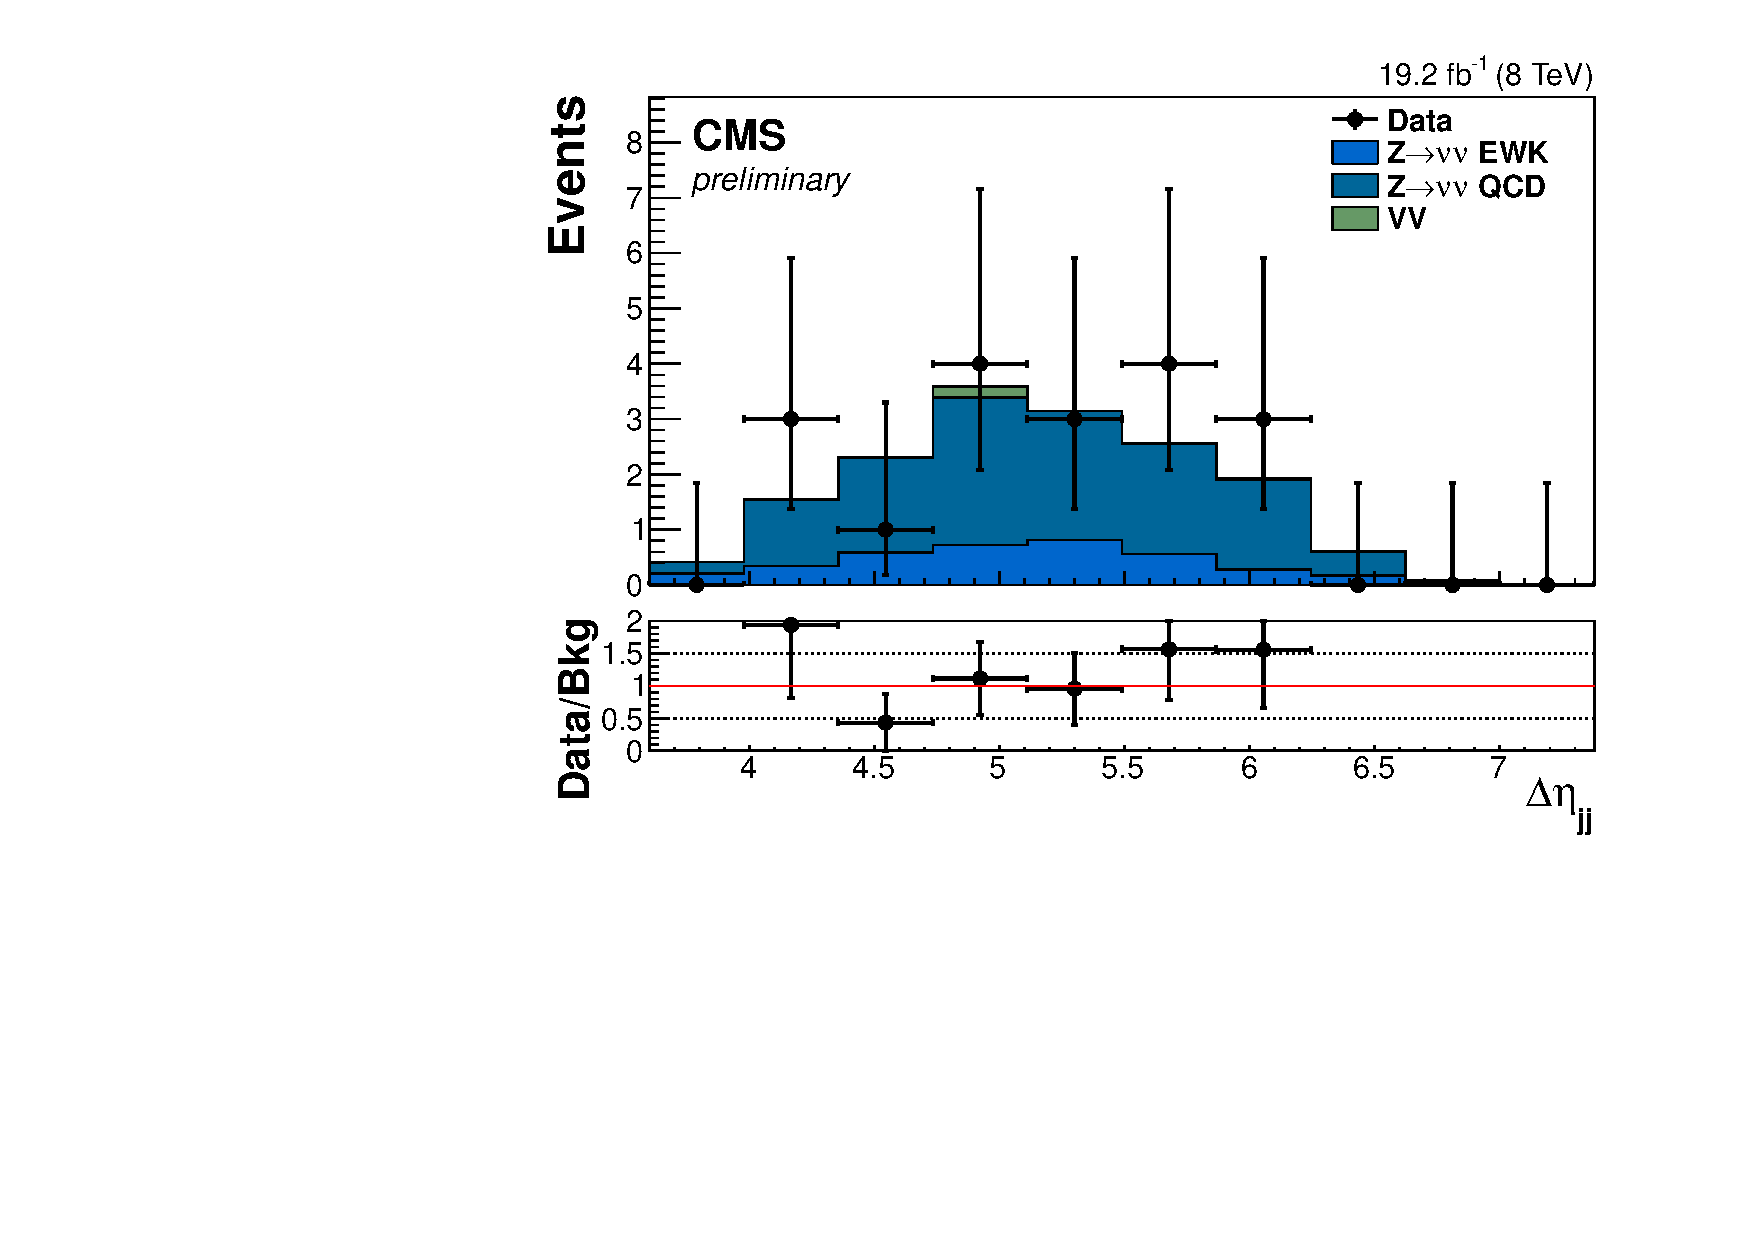
\includegraphics[width=.49\textwidth]{Chapter07/Images/output_sigreg/mumu_dijet_deta.pdf}}
\subfloat[]{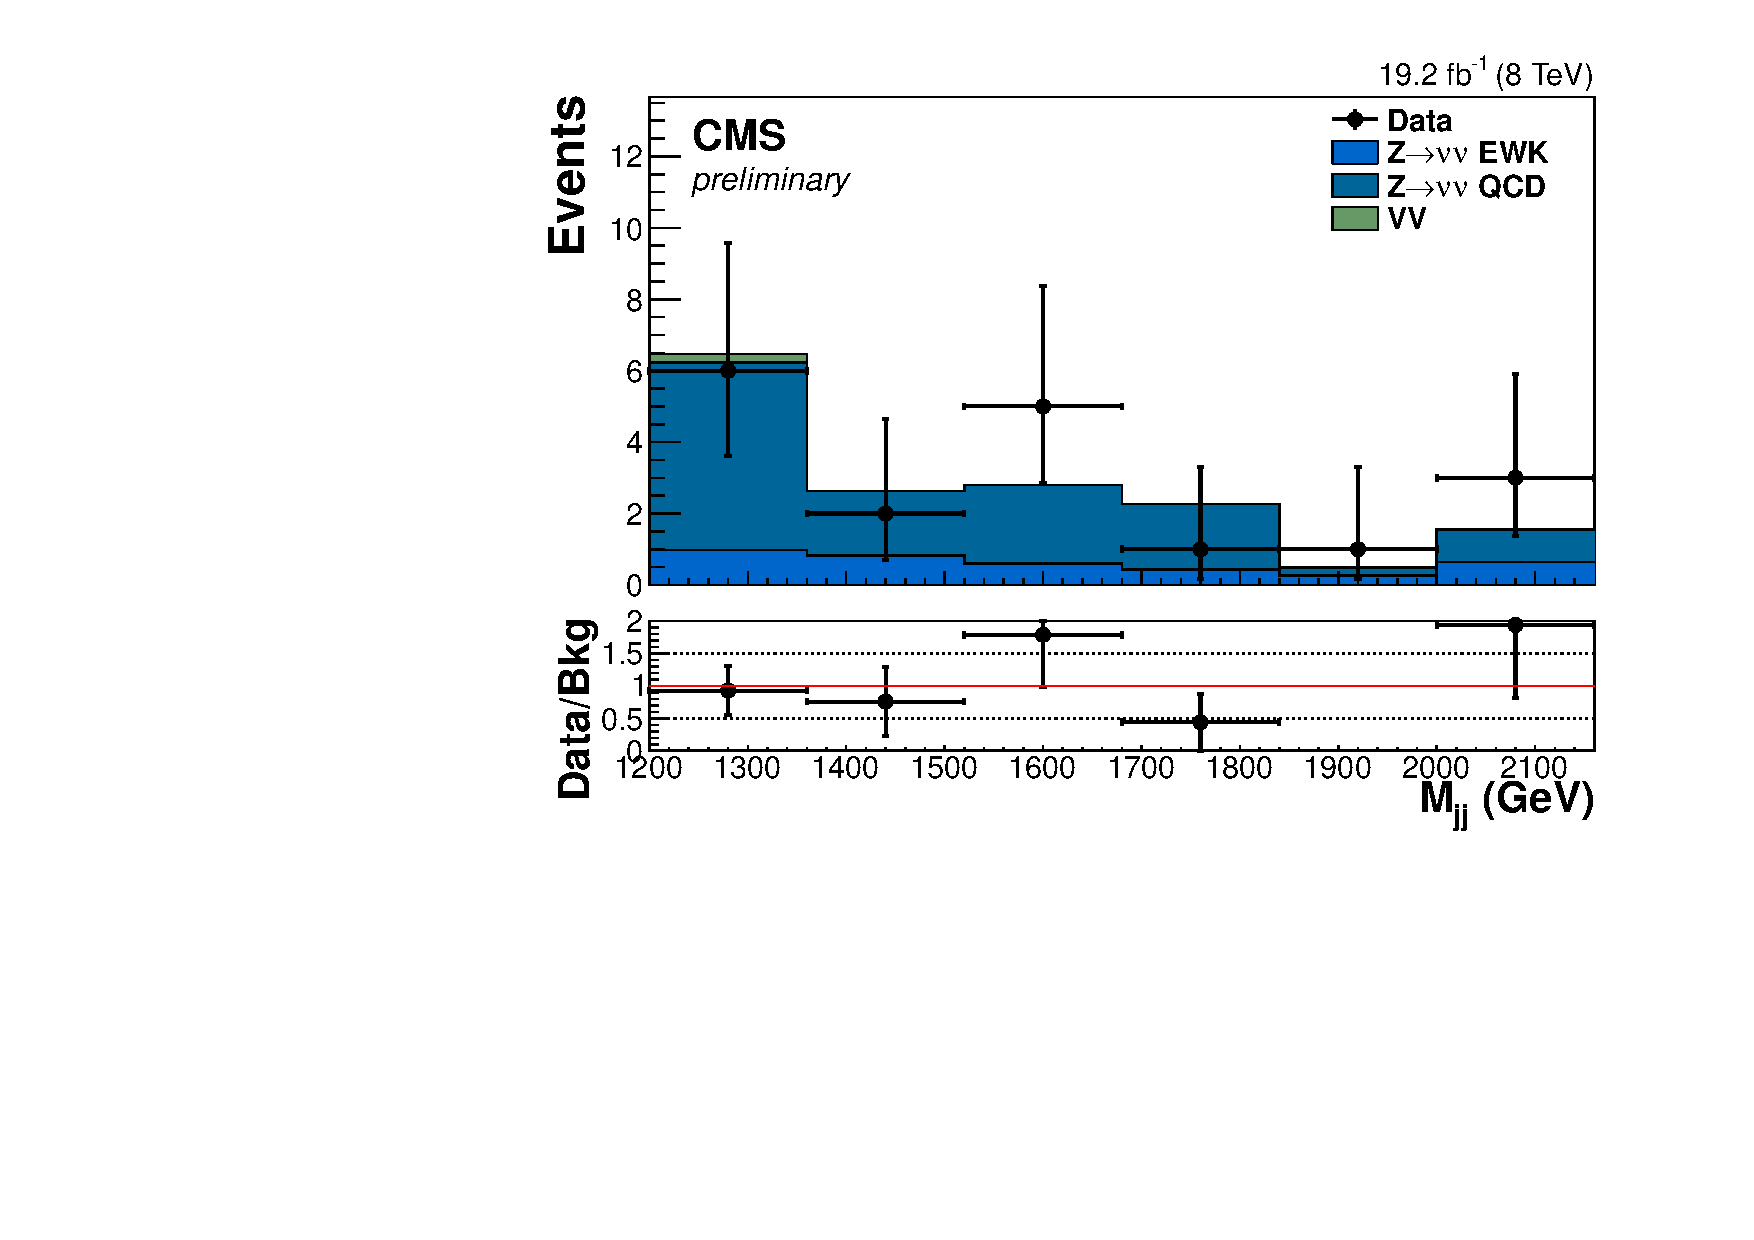
\includegraphics[width=.49\textwidth]{Chapter07/Images/output_sigreg/mumu_dijet_M.pdf}} \\
\subfloat[]{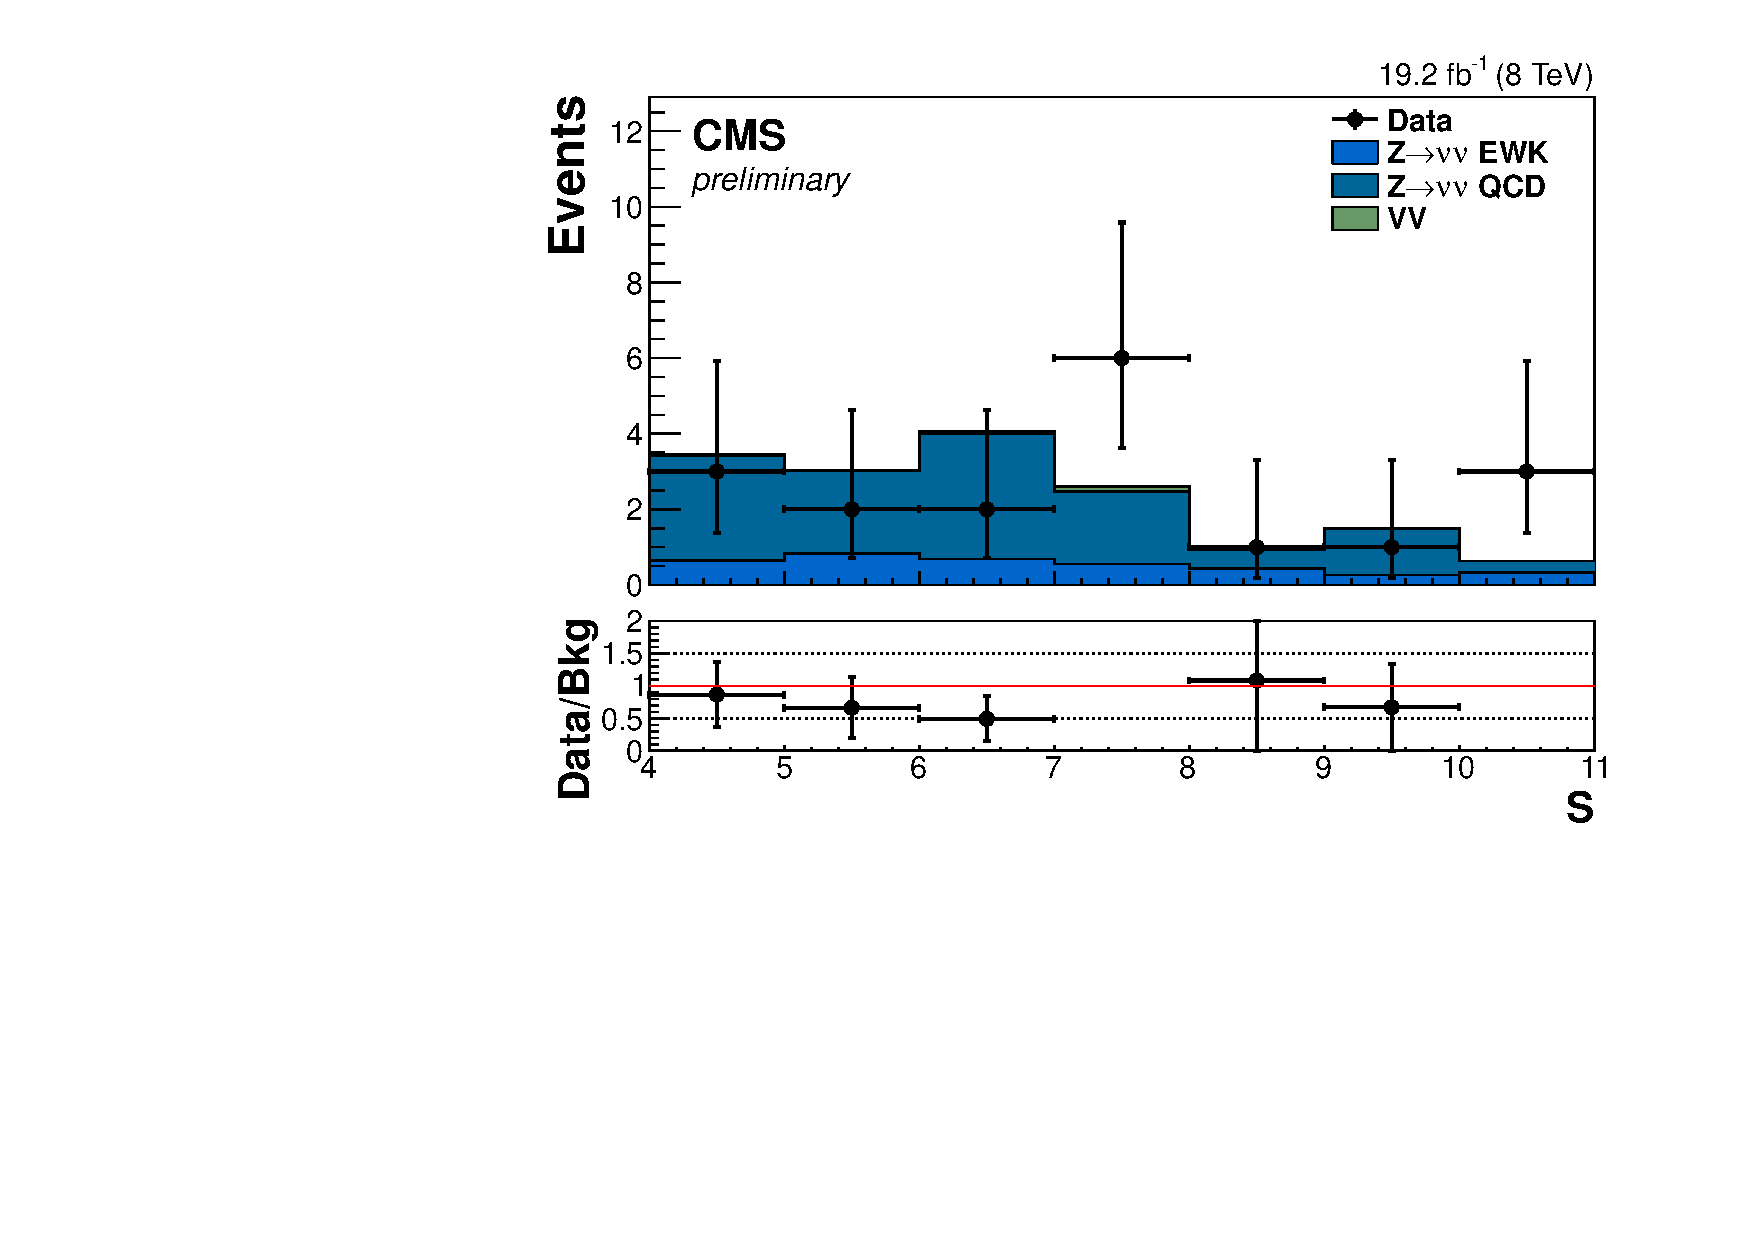
\includegraphics[width=.49\textwidth]{Chapter07/Images/output_sigreg/mumu_metnomu_significance.pdf}}
\subfloat[]{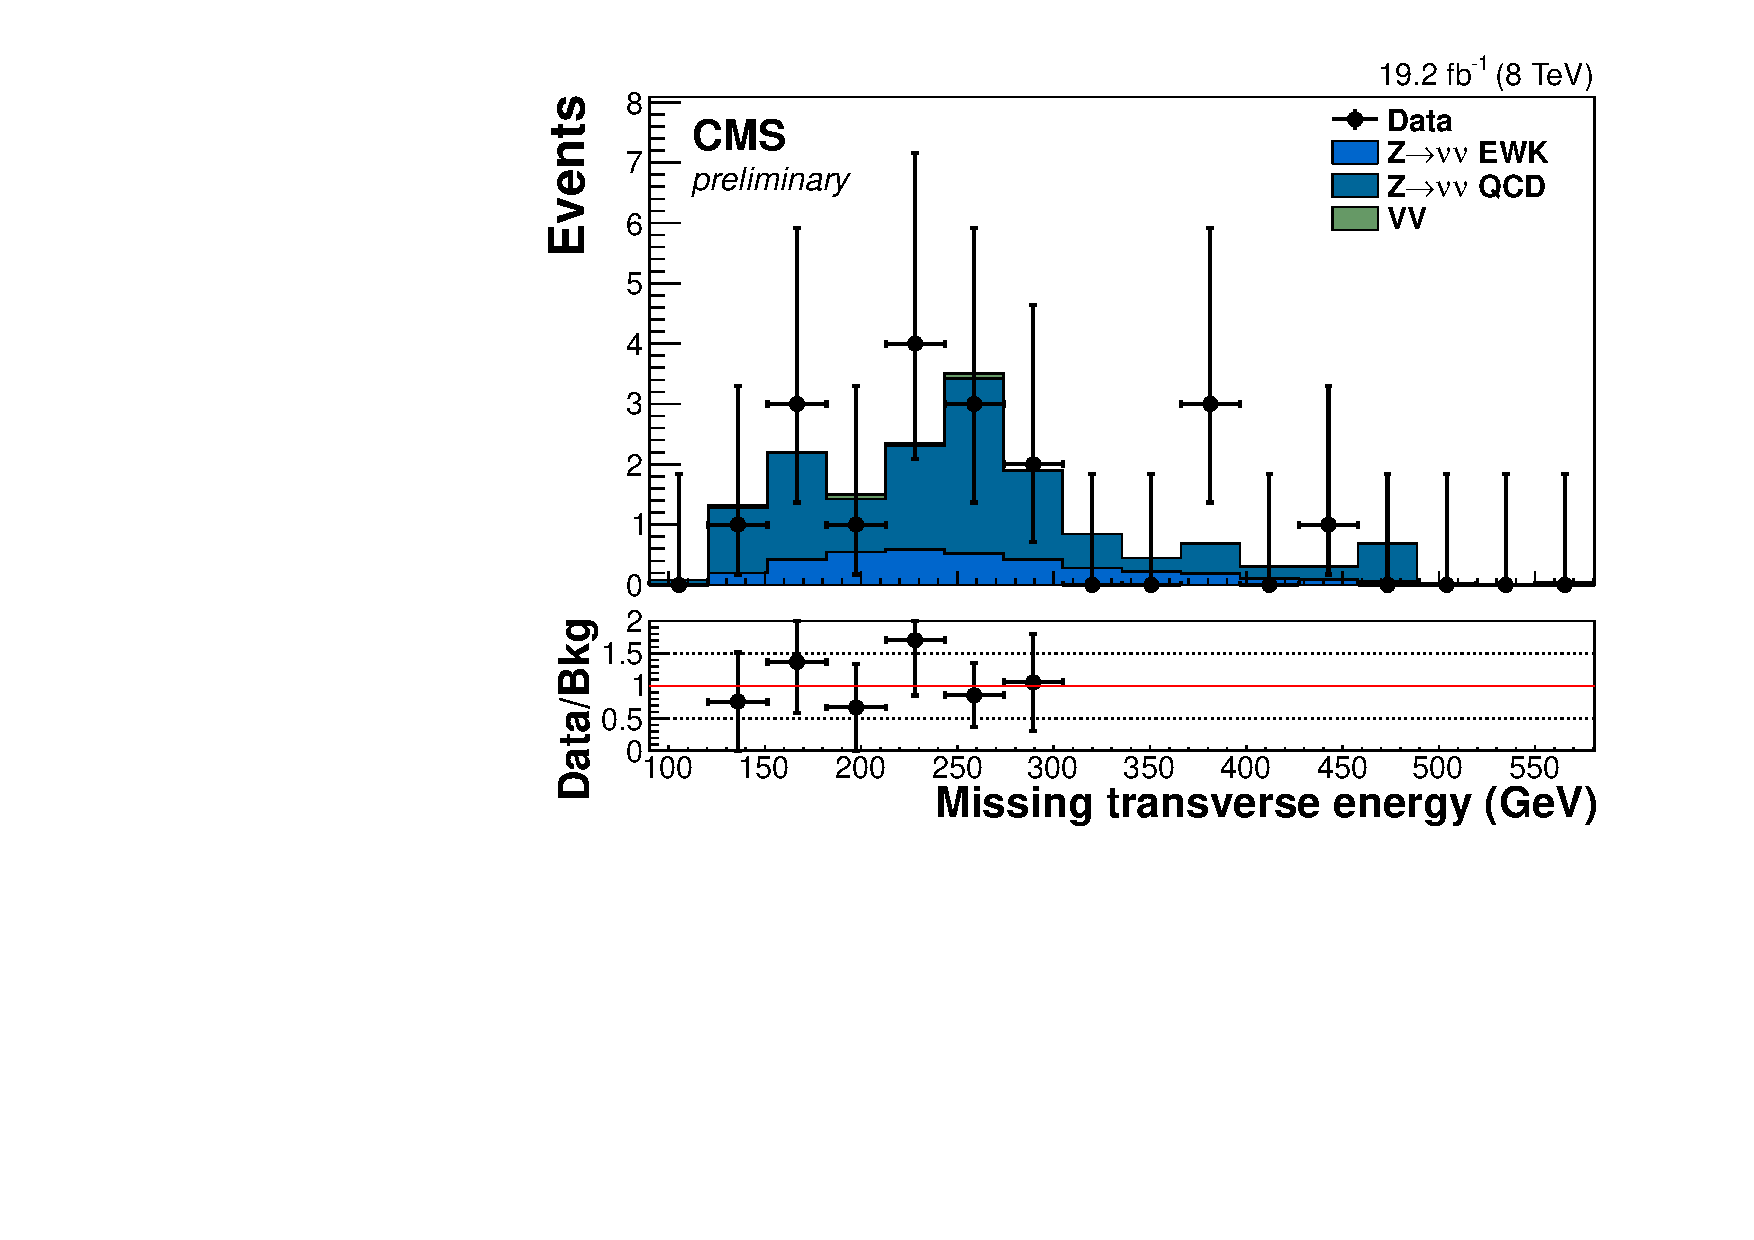
\includegraphics[width=.49\textwidth]{Chapter07/Images/output_sigreg/mumu_metnomuons.pdf}}
\caption{Distributions of (a) Pseudorapidity difference between the two selected \gls{VBF} jets, $\Delta\eta_{jj}$, (b) Dijet mass $M_{jj}$, (c) \gls{MET} significance $\mathcal{S}$, (d) and \gls{MET}, in the $Z\rightarrow \mu\mu$ control region. The last bin contains the overflow of the distribution \cite{ARTICLE:CMSVBFHiggsInvisibleParkedAnalysisPAS}.}
\label{FIGURE:ParkedDataAnalysis_ZBackground_KeyDistributions}
\end{figure}

Good agreement between data and \gls{MC} simulation is observed considering the available statistics. The final estimation of the contribution of the $Z\rightarrow \nu\nu$ background to the signal region is $N_{S}^{Z\rightarrow\nu\nu}= 158.1 \pm 37.8 \stat \pm 21.2 \syst$.

%%%%%%%%%%%%%%%%%%%%%%%%%%%%%%%%%%%%%%%%%%%%%%%%%%%%%%%%%%%%%%%%%%%%%%%%%%%%%%%%%%%%
%%% SUBSECTION
%%%%%%%%%%%%%%%%%%%%%%%%%%%%%%%%%%%%%%%%%%%%%%%%%%%%%%%%%%%%%%%%%%%%%%%%%%%%%%%%%%%%
\subsection{W background estimation}
\label{SECTION:ParkedDataAnalysis_ControlRegions_WBackground}

%Status: DONE (reviewed J.Pela x1)

A similar approach is taken for the W background, the control region is defined by the signal region criteria except that we explicitly require the presence of exactly one single lepton (tight electron or tight muon) or hadronic tau and no other additional leptons. The data event yield obtained in this region is extrapolated to the signal region with a conversion factor determined from \gls{MC} simulation. Equation \ref{EQUATION:ParkedDataAnalysis_WBackground} is used to obtain the predicted number of events in the signal region.

\begin{align}
%   \begin{split}
%   \end{split}
N_{S}^{W}&=N_{S}^{W\,MC}\frac{N_{C}^{Data}-N_{C}^{bkg}}{N_{C}^{W\,MC}}=N_{S}^{W\,MC}\cdot \rm{SF}
\label{EQUATION:ParkedDataAnalysis_WBackground}
\end{align}

The prediction of each W decay channel is calculated separately for e, $\mu$ (which include $W\rightarrow\tau\nu\rightarrow \nu_\tau l\nu_l$ with $l$ equal to e and $\mu$ respectively) and hadronic $\tau$. In these control region the number of events from other background $N_{C}^{bkg}$ is mainly composed of event from top processes which are estimated from \gls{MC}.

In the W$\rightarrow\tau_{\mathrm{h}}\nu$ control region a very small amount of events passes the $\Delta\phi(\text{MET},jets)$ requirement. In order to increase event statistics it is replaces by a requirement on the minimal azimuthal angle separation between the \gls{MET} and one of the leading two jets $\Delta\phi(\text{MET},jet_{1,2})$ greater than 1. To reject events from \gls{QCD} multi-jet processes an additional requirement on the transverse mass of the W to be greater than $20\,\GeV$ is used. The W$\rightarrow\mu\nu$ region has enough statistics to study the full range of $\Delta\phi(\text{MET},jets)$, a 20\% systematic uncertainty is added to account for the observed difference in shape of the $\Delta\phi(\text{MET},jets)$ variable observed between \gls{MC} simulation and data. Distributions of $M_{jj}$, \gls{MET} and $\Delta\phi(\text{MET},jets)$ are shown in figures \ref{FIGURE:ParkedDataAnalysis_WBackground_Mjj}, \ref{FIGURE:ParkedDataAnalysis_WBackground_MetNoMu} and \ref{FIGURE:ParkedDataAnalysis_WBackground_MinDeltaPhi}

\begin{figure}[!htb]
\centering
\subfloat[]{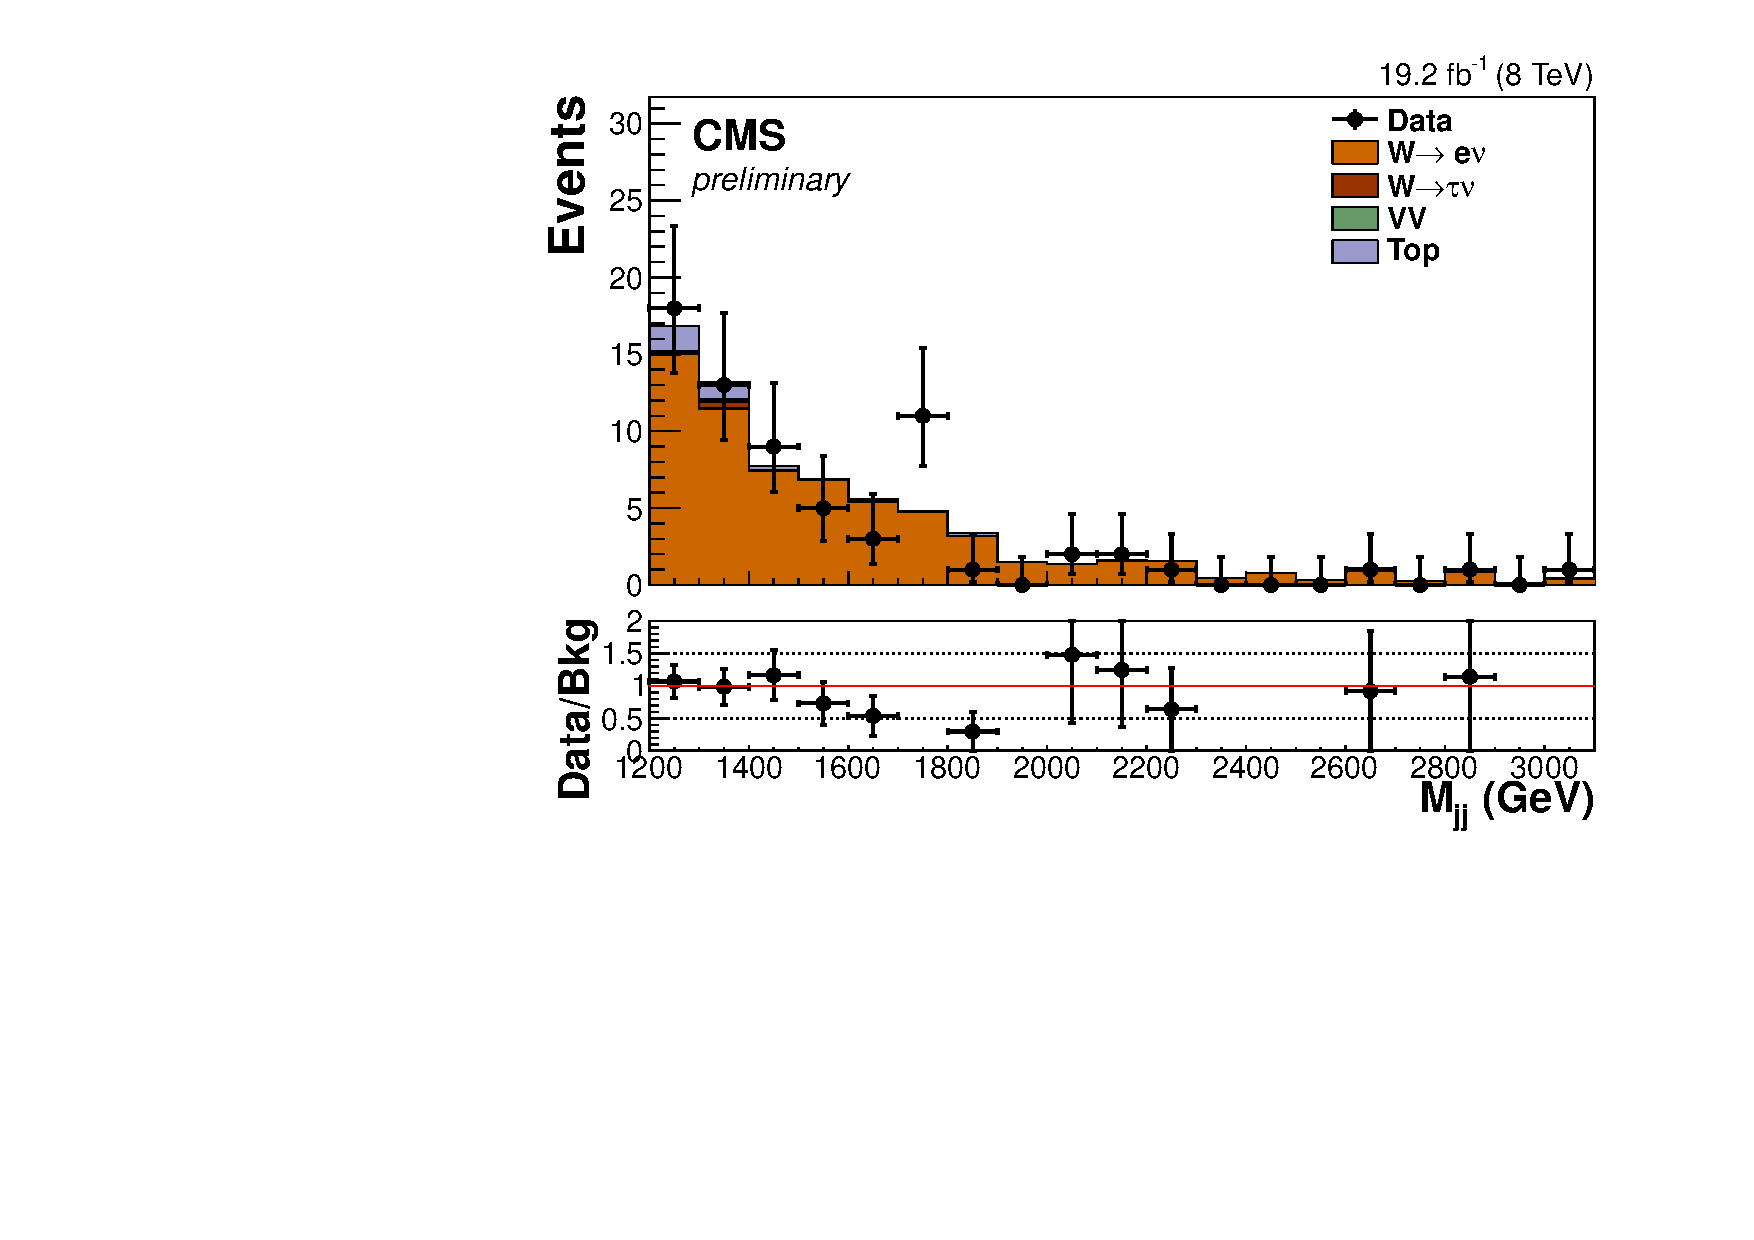
\includegraphics[width=.45\textwidth]{Chapter07/Images/output_sigreg/enu_dijet_M.pdf}}
\subfloat[]{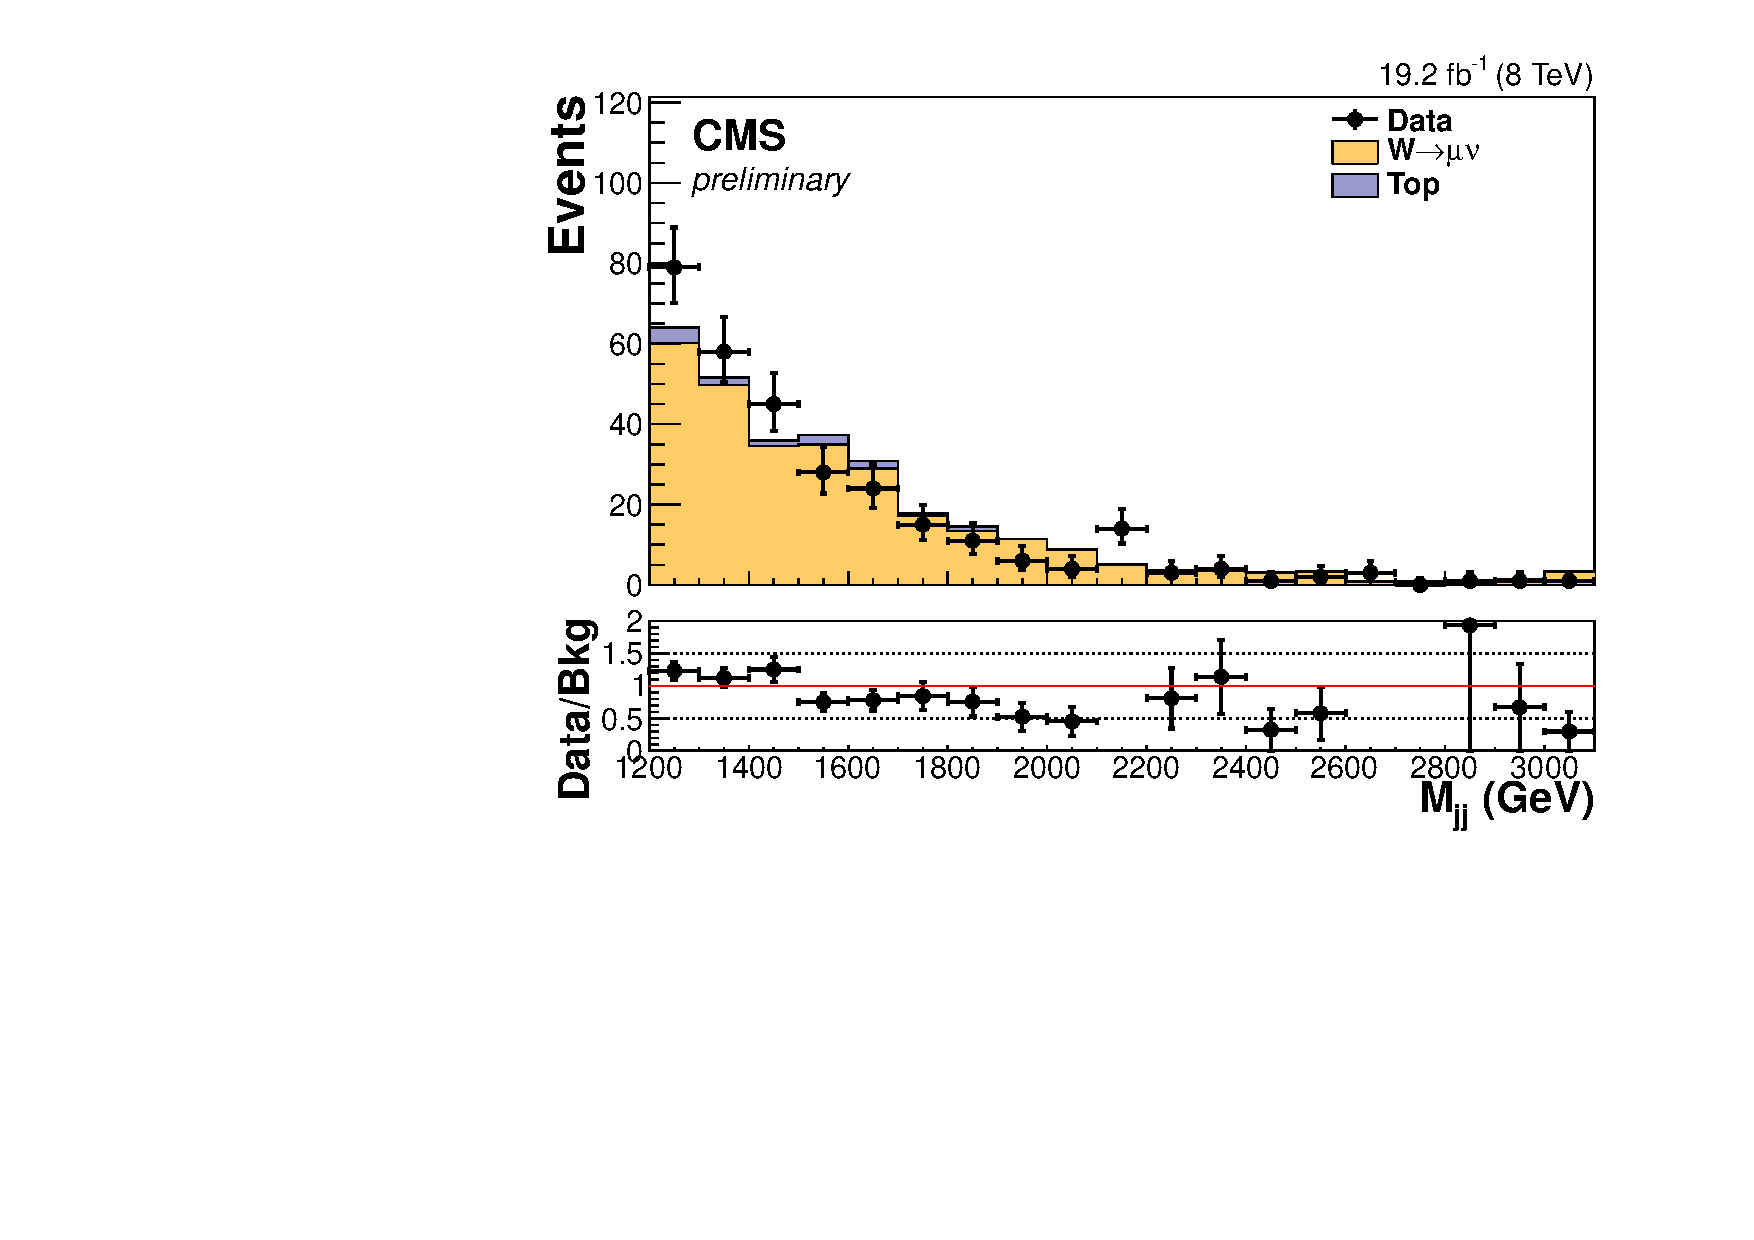
\includegraphics[width=.45\textwidth]{Chapter07/Images/output_sigreg/munu_dijet_M.pdf}} \\
\subfloat[]{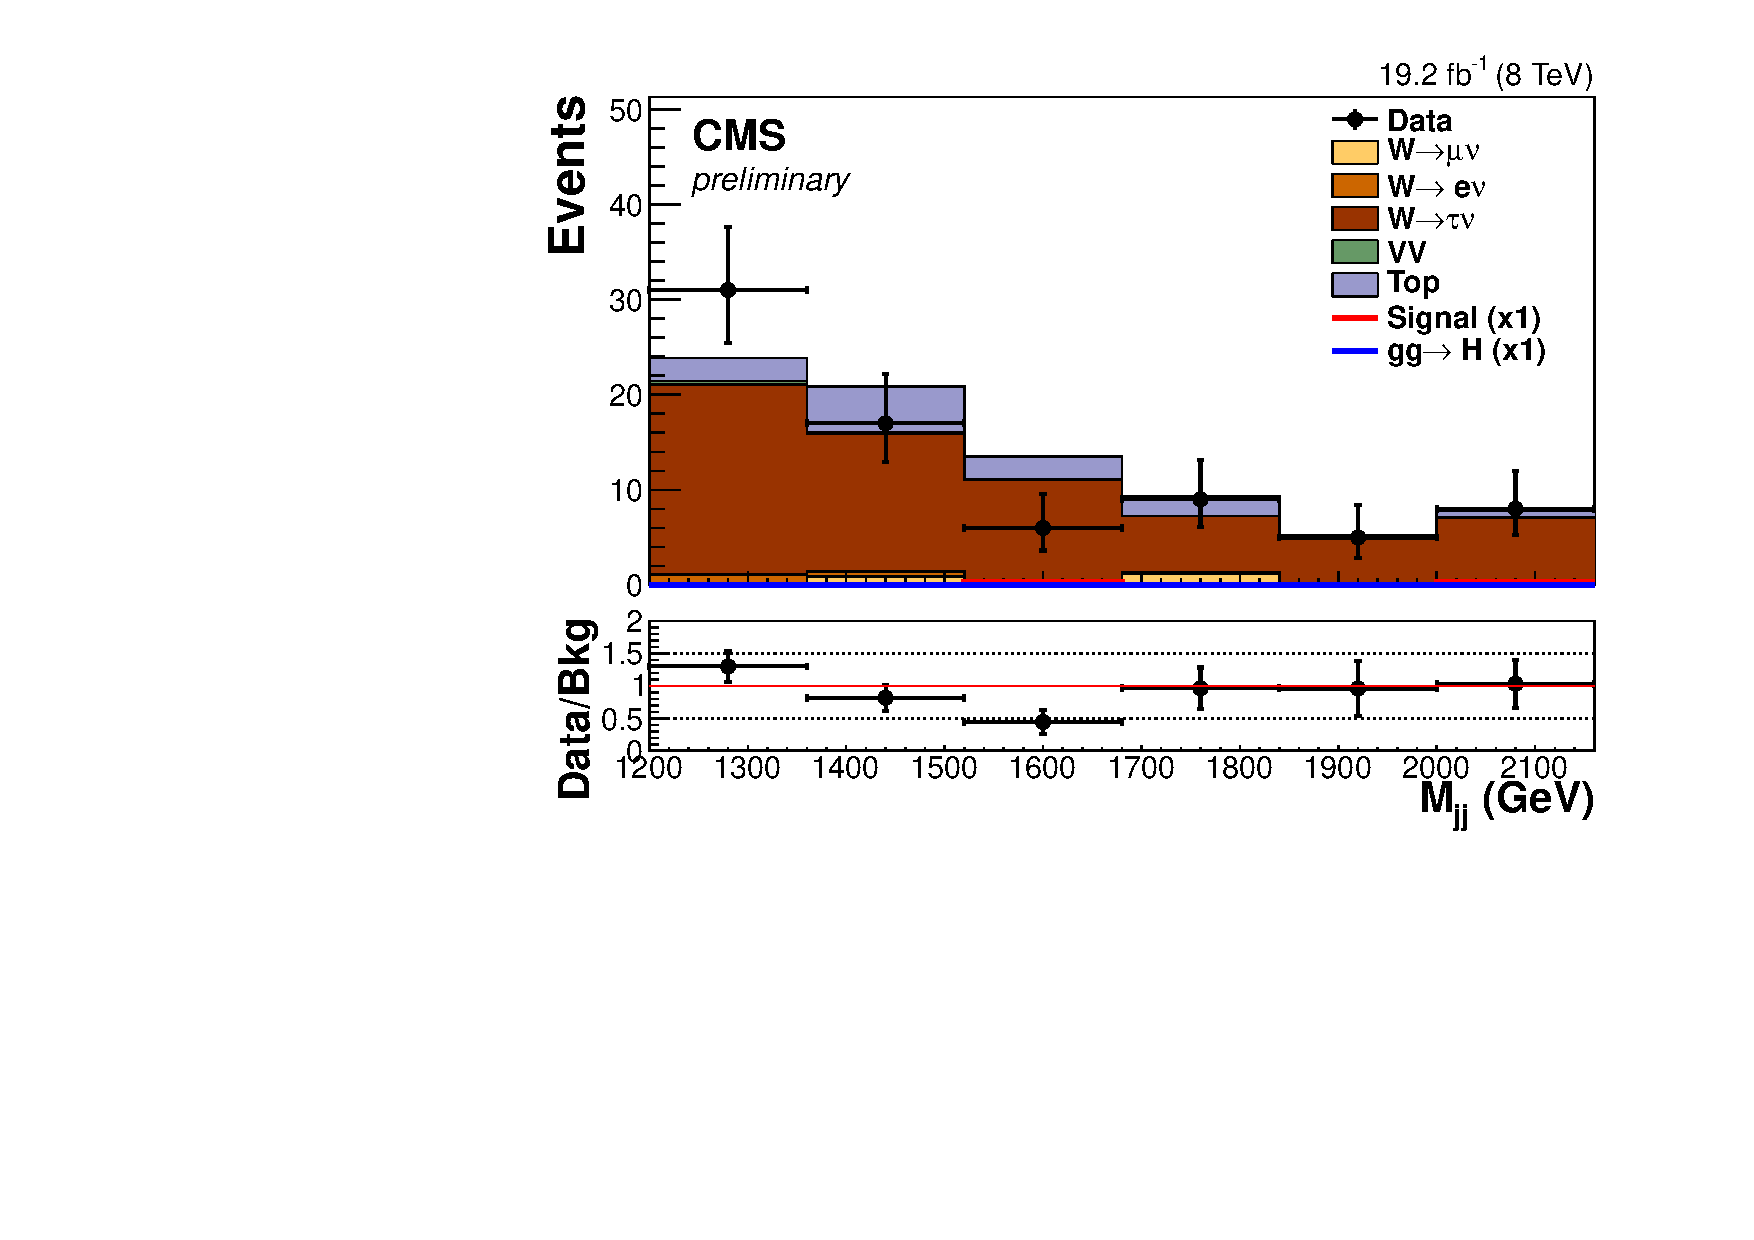
\includegraphics[width=.45\textwidth]{Chapter07/Images/output_sigreg/taunu_dijet_M.pdf}}
\caption{Dijet mass $M_{jj}$ for the (a) $W\rightarrow e\nu$, (b) $W\rightarrow\mu\nu$ and (c) $W\rightarrow\tau\nu$ control regions. The last bin represents all those events falling above the range of the histogram \cite{ARTICLE:CMSVBFHiggsInvisibleParkedAnalysisPAS}.}
\label{FIGURE:ParkedDataAnalysis_WBackground_Mjj}
\end{figure}

\begin{figure}[!htb]
\centering
\subfloat[]{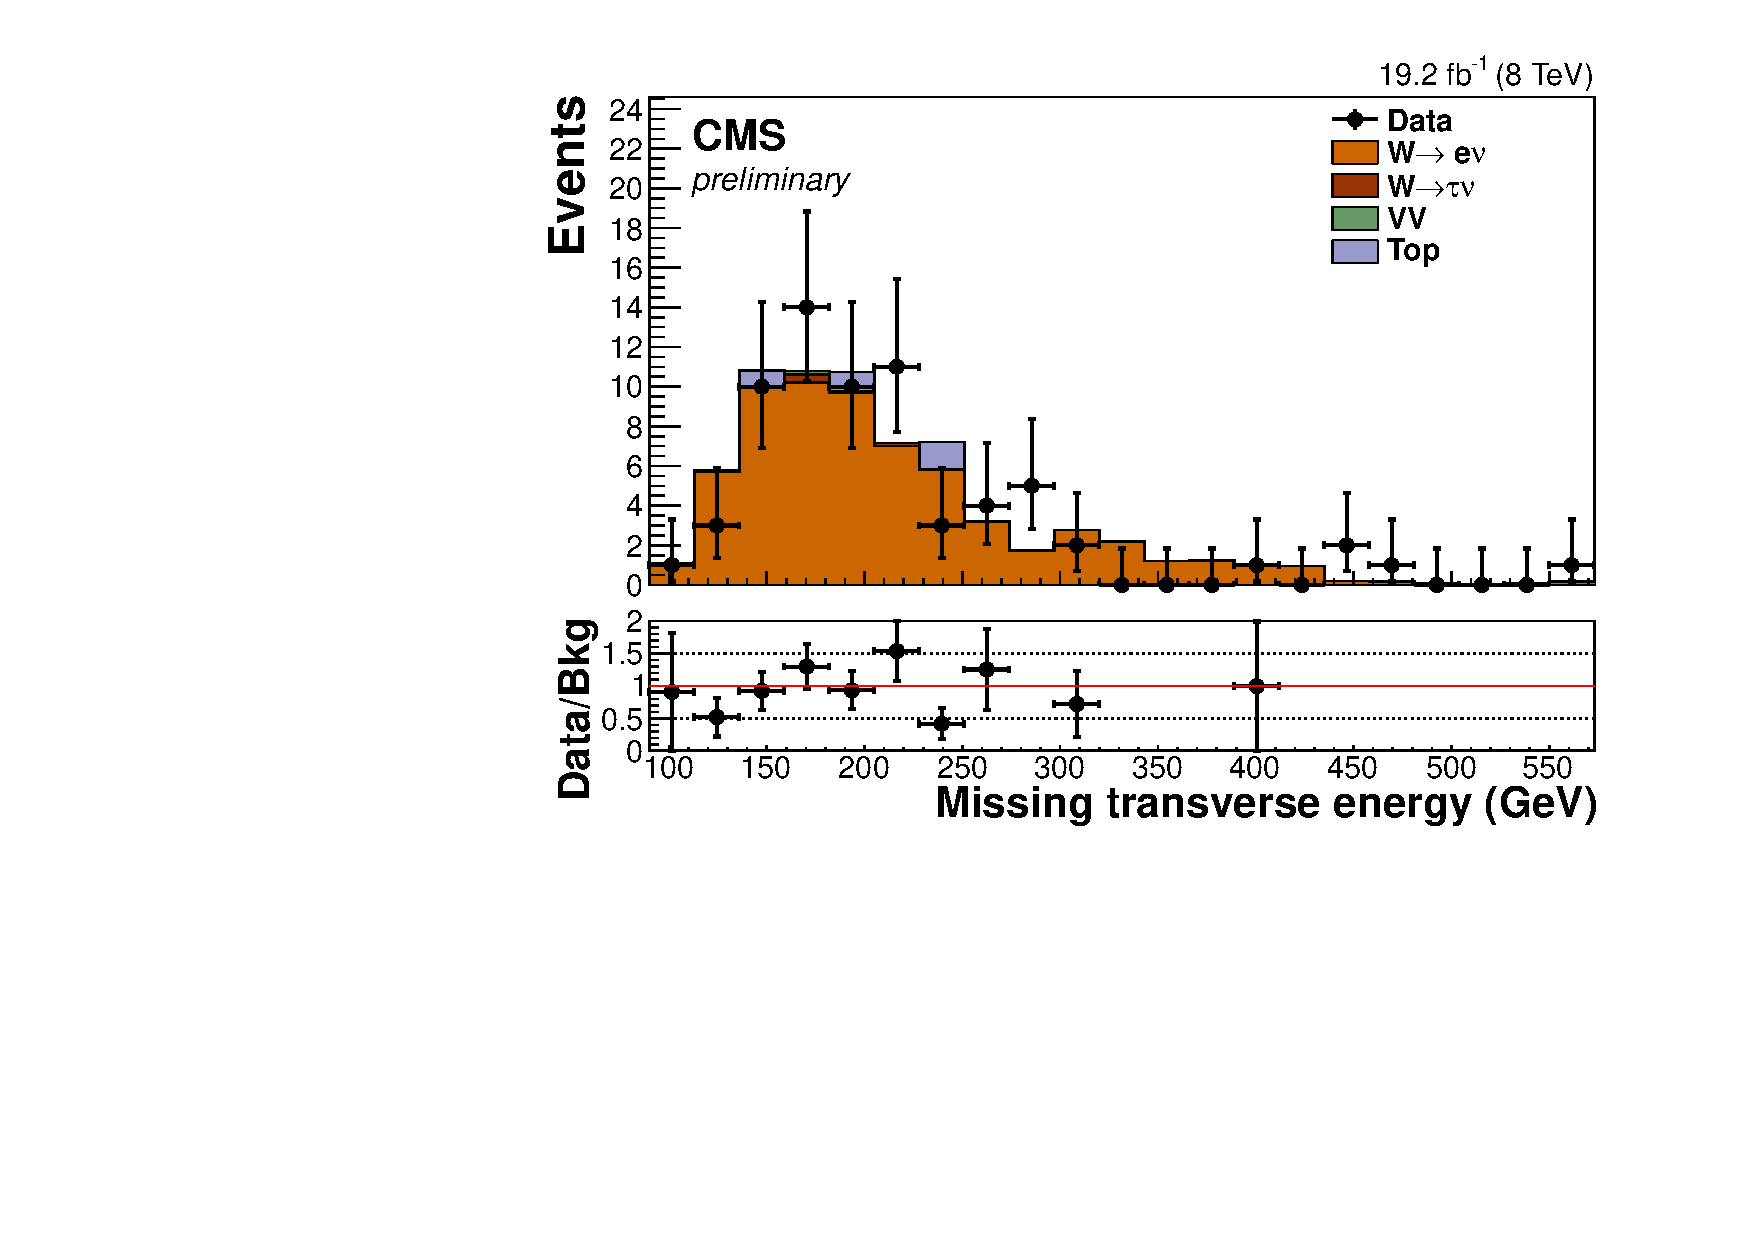
\includegraphics[width=.45\textwidth]{Chapter07/Images/output_sigreg/enu_metnomuons.pdf}}
\subfloat[]{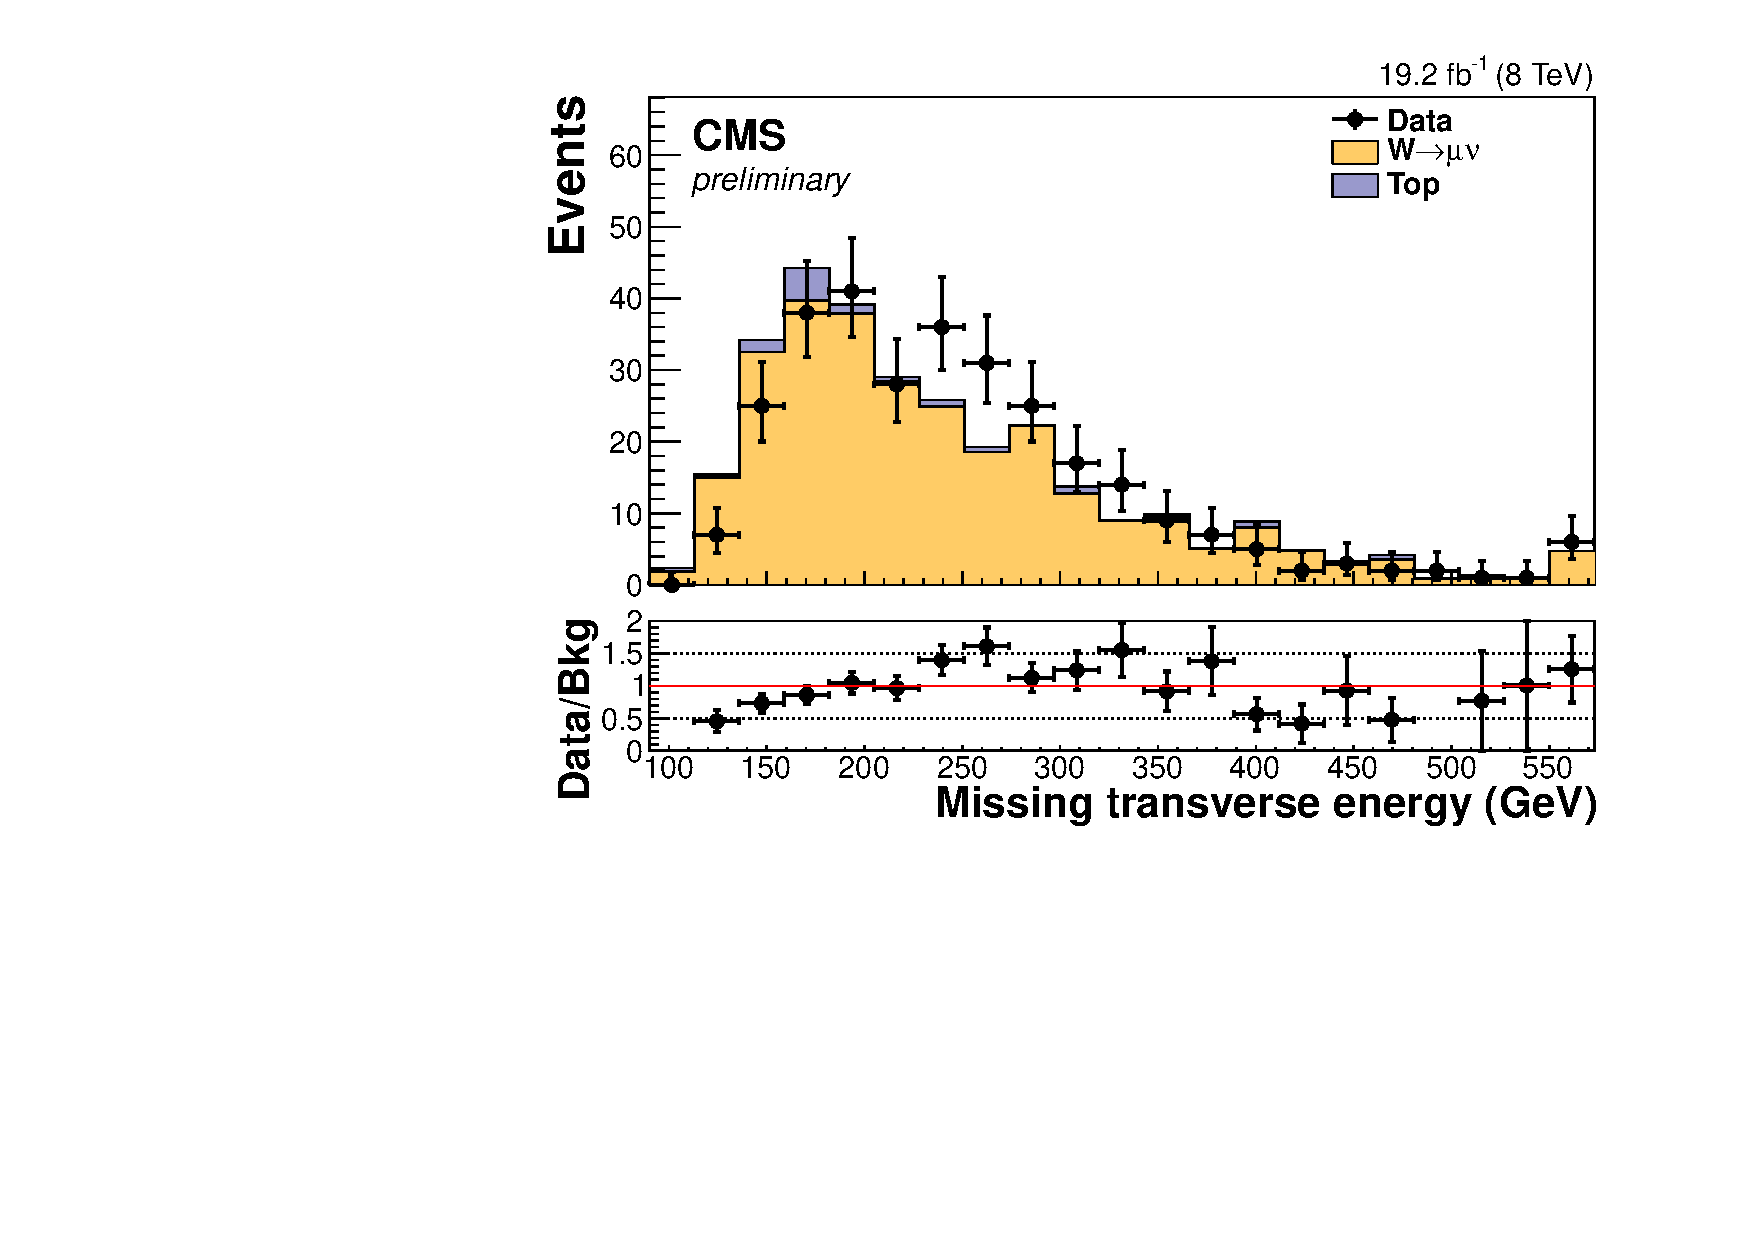
\includegraphics[width=.45\textwidth]{Chapter07/Images/output_sigreg/munu_metnomuons.pdf}} \\
\subfloat[]{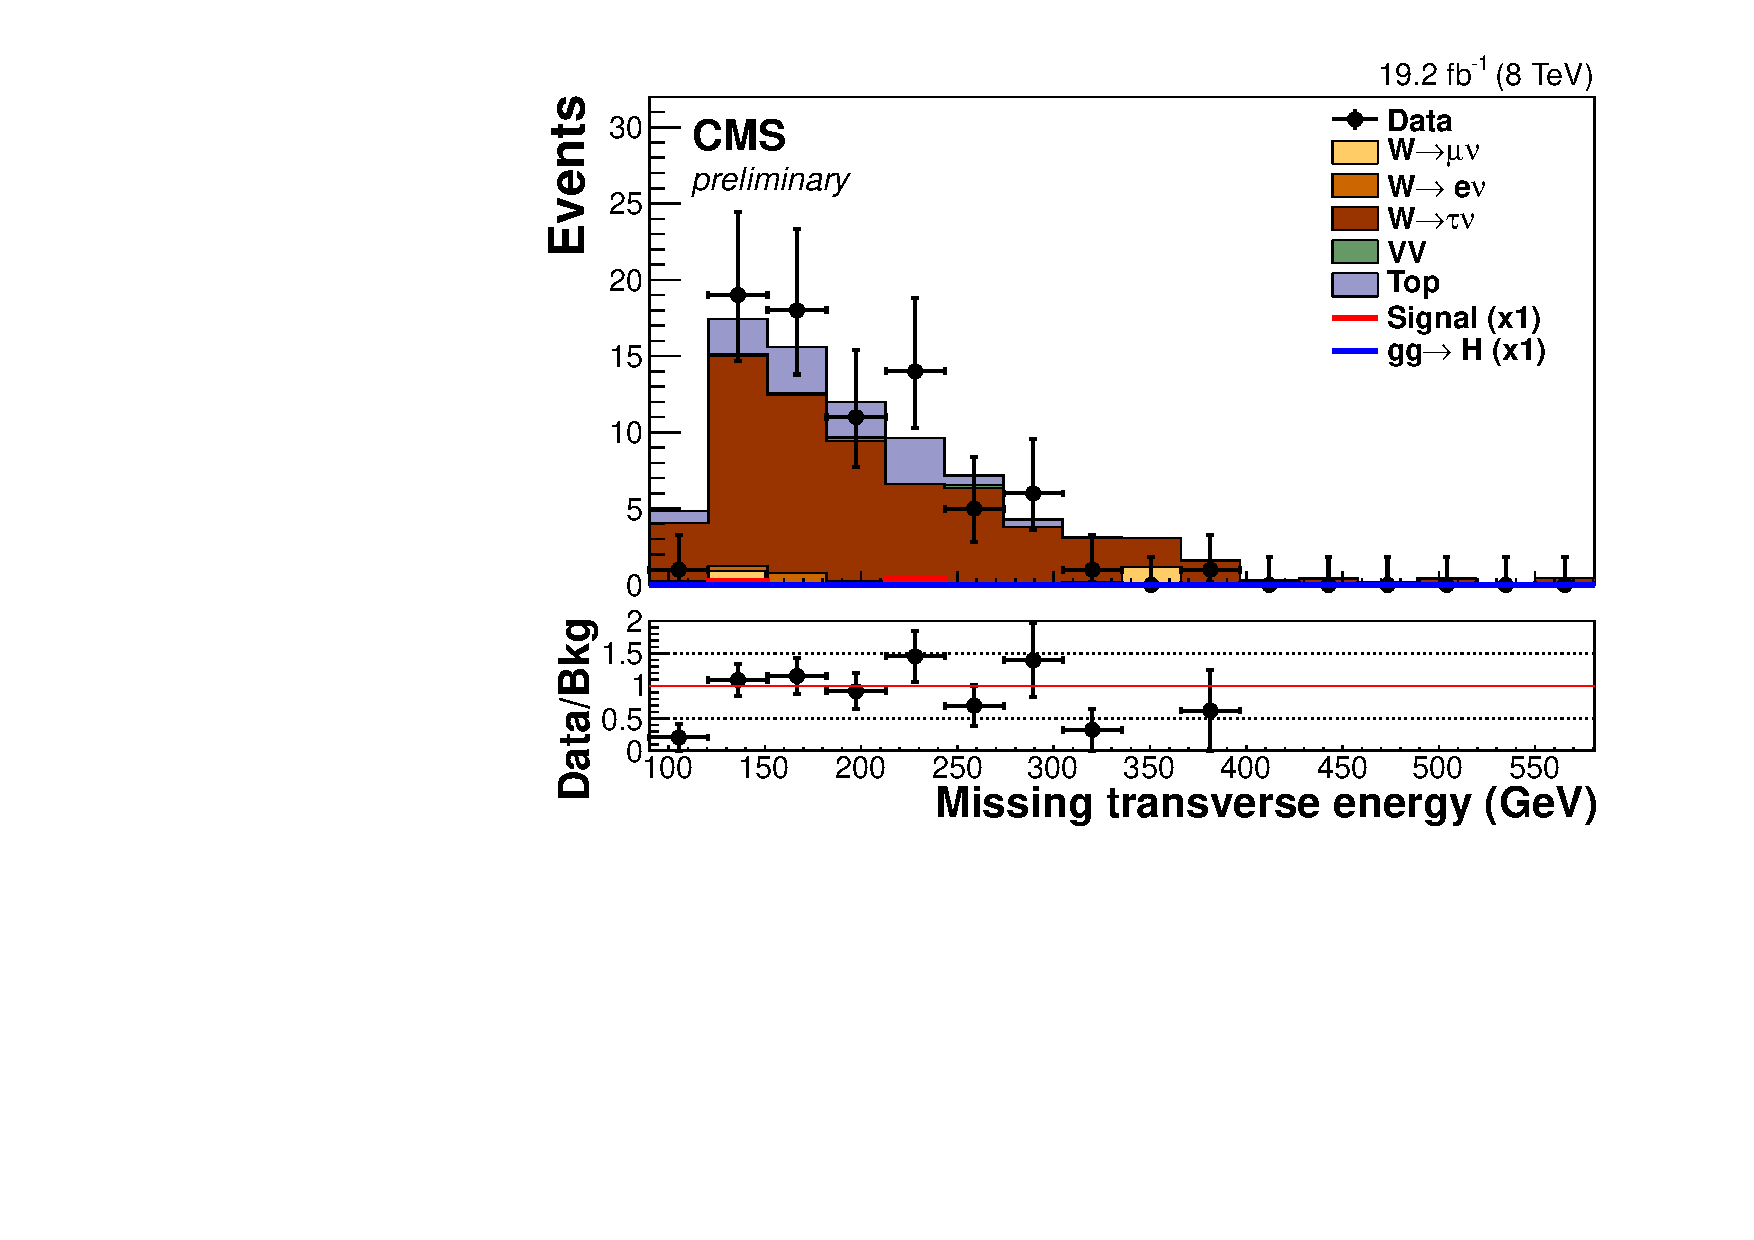
\includegraphics[width=.45\textwidth]{Chapter07/Images/output_sigreg/taunu_metnomuons.pdf}}
\caption{\gls{MET} for the (a) $W\rightarrow e\nu$, (b) $W\rightarrow\mu\nu$ and (c) $W\rightarrow\tau\nu$ control regions. The last bin represents all those events falling above the range of the histogram \cite{ARTICLE:CMSVBFHiggsInvisibleParkedAnalysisPAS}.}
\label{FIGURE:ParkedDataAnalysis_WBackground_MetNoMu}
\end{figure}

\begin{figure}[!htb]
\centering
\subfloat[]{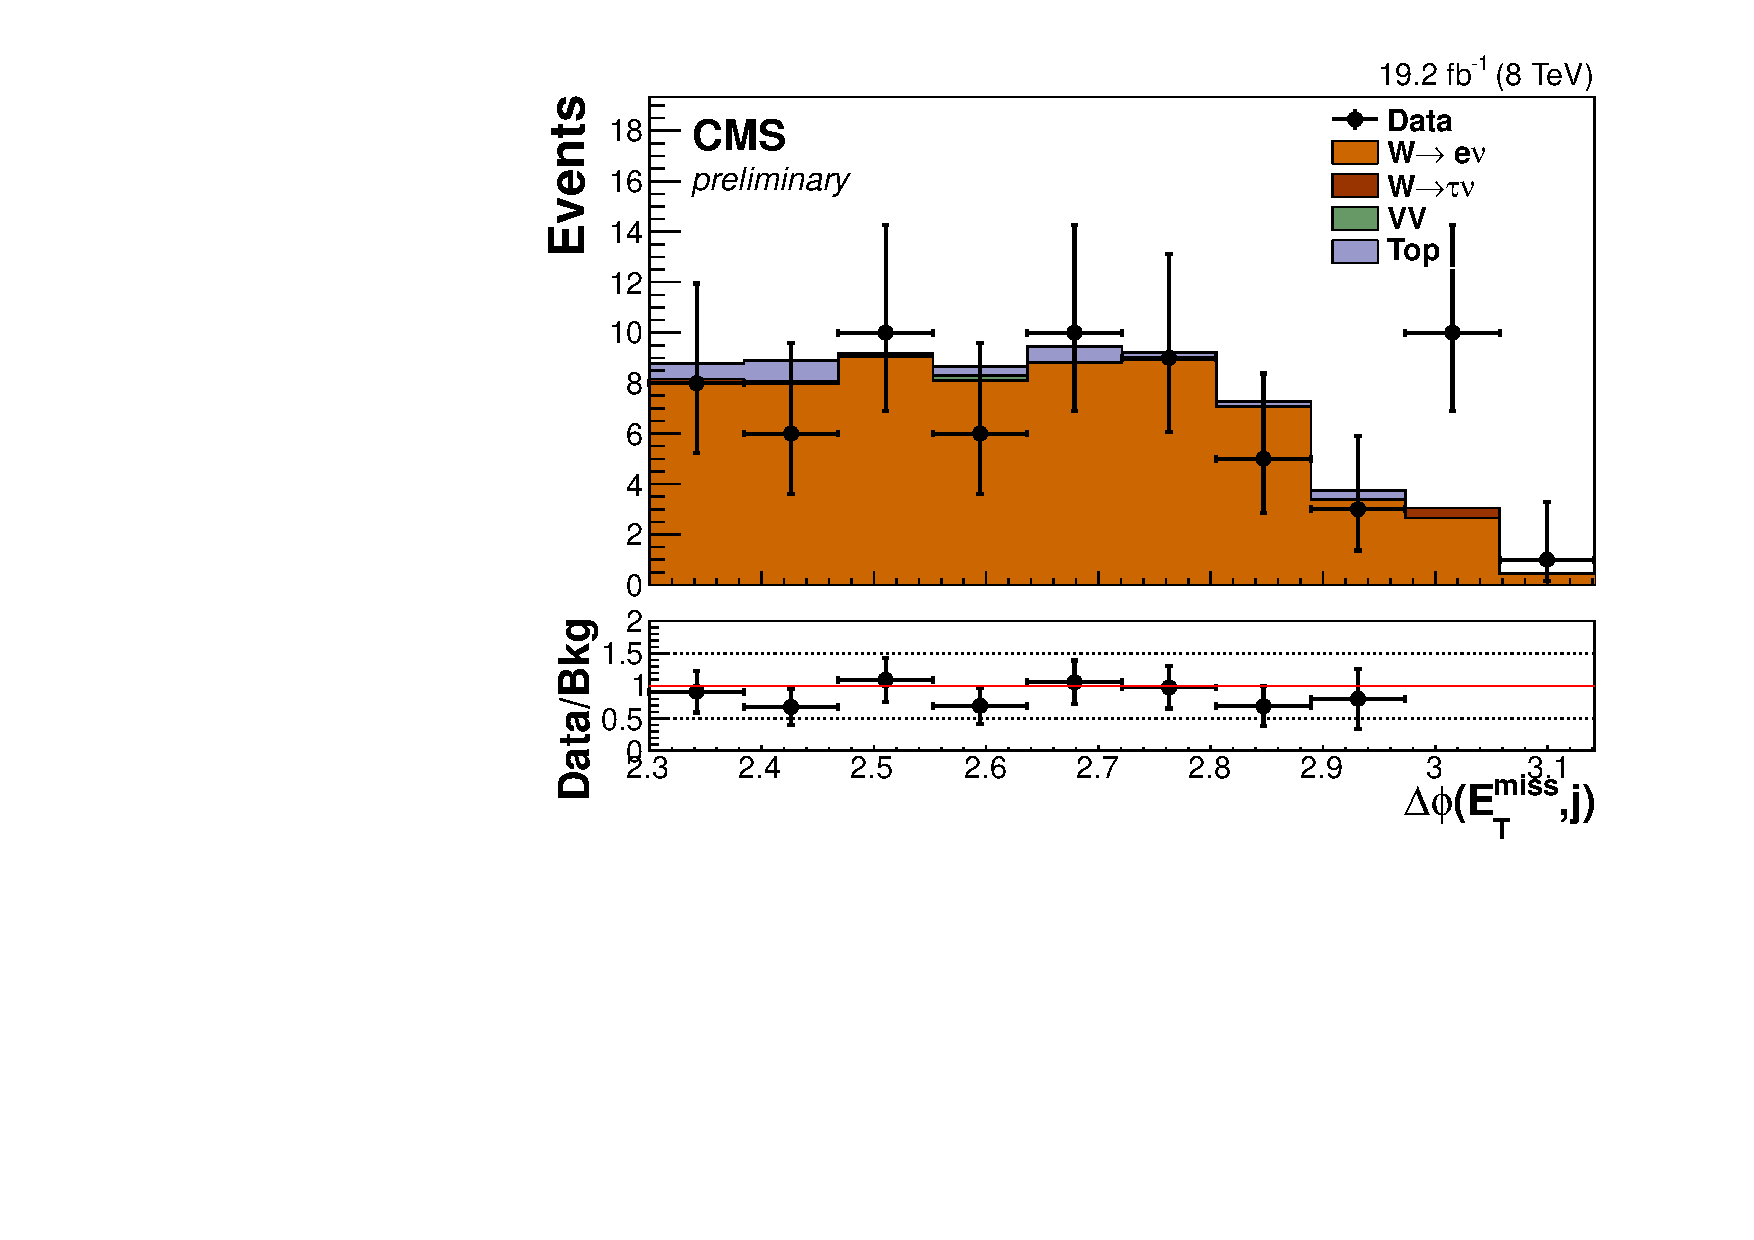
\includegraphics[width=.45\textwidth]{Chapter07/Images/output_sigreg/enu_alljetsmetnomu_mindphi.pdf}}
\subfloat[]{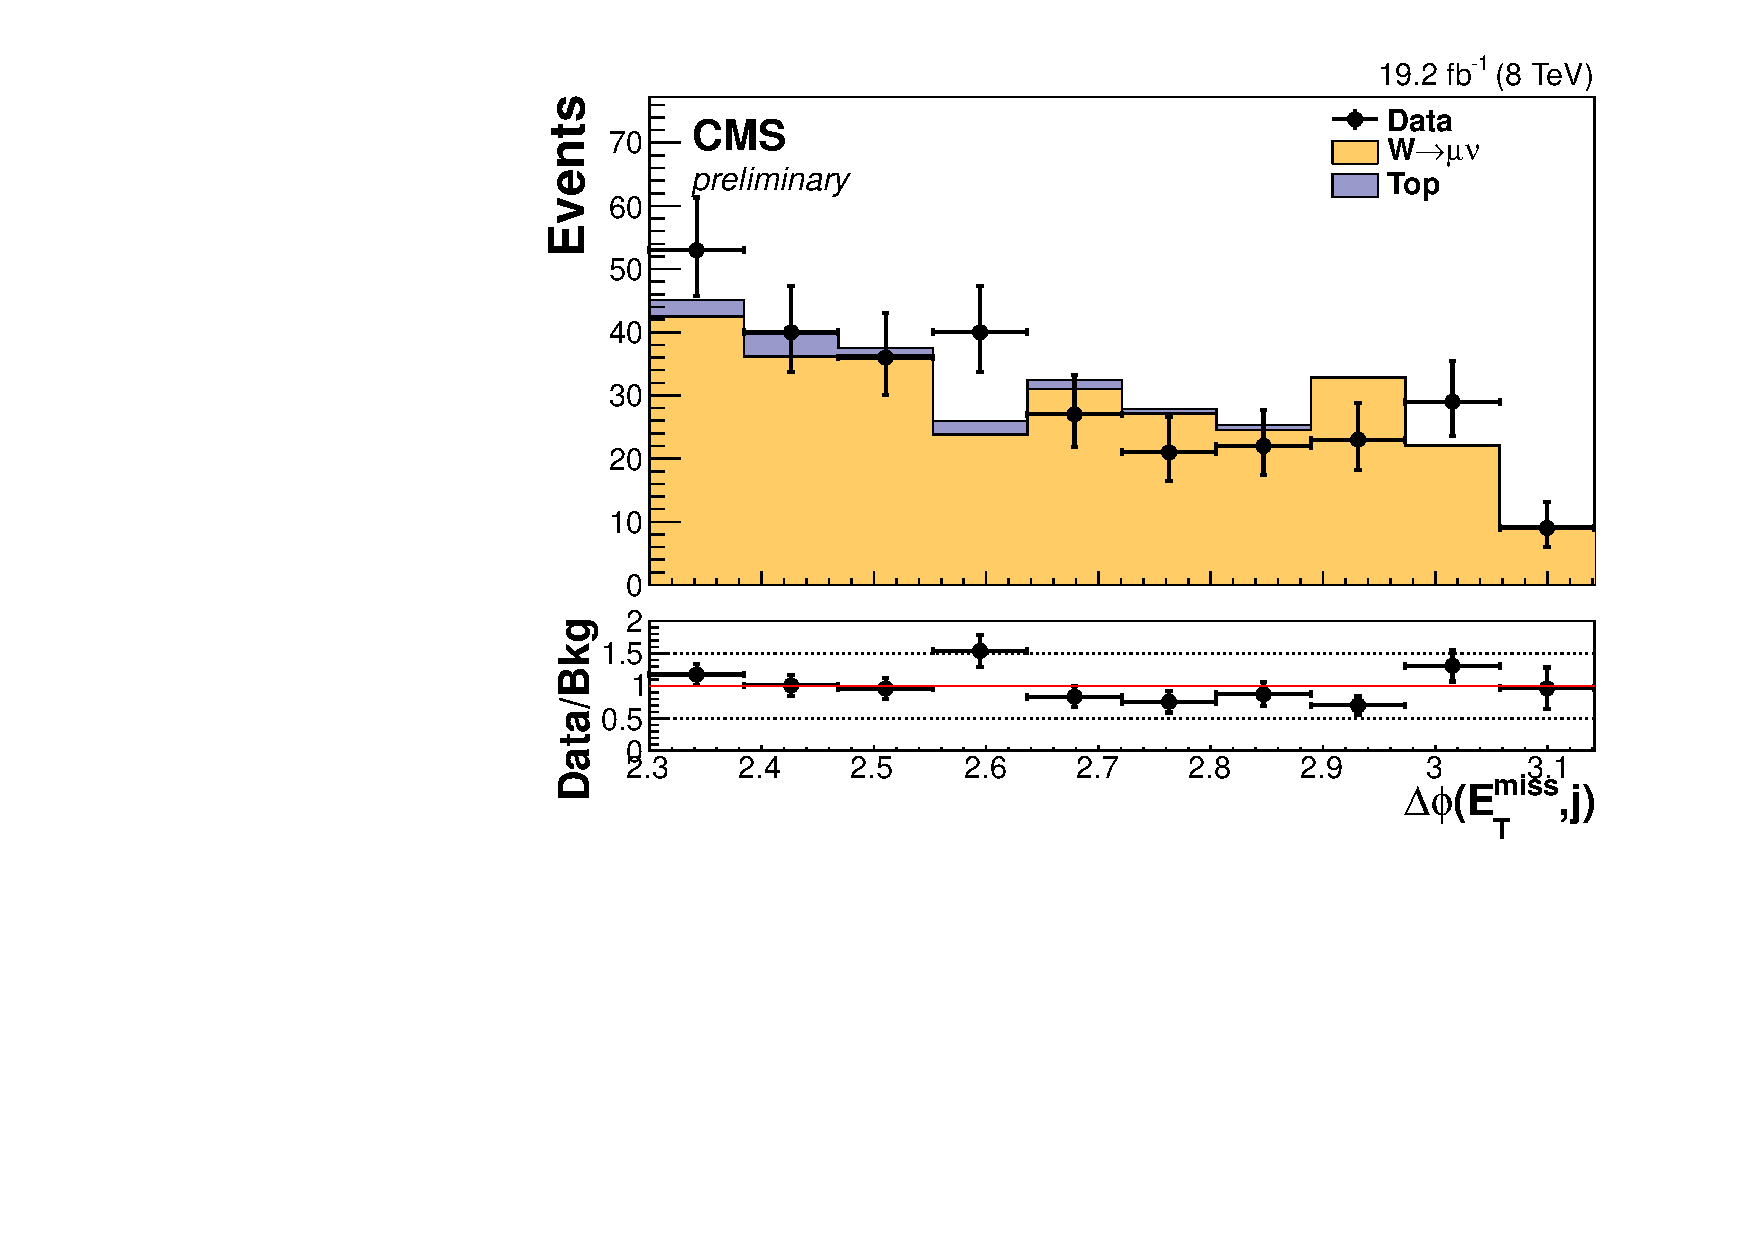
\includegraphics[width=.45\textwidth]{Chapter07/Images/output_sigreg/munu_alljetsmetnomu_mindphi.pdf}} \\
\subfloat[]{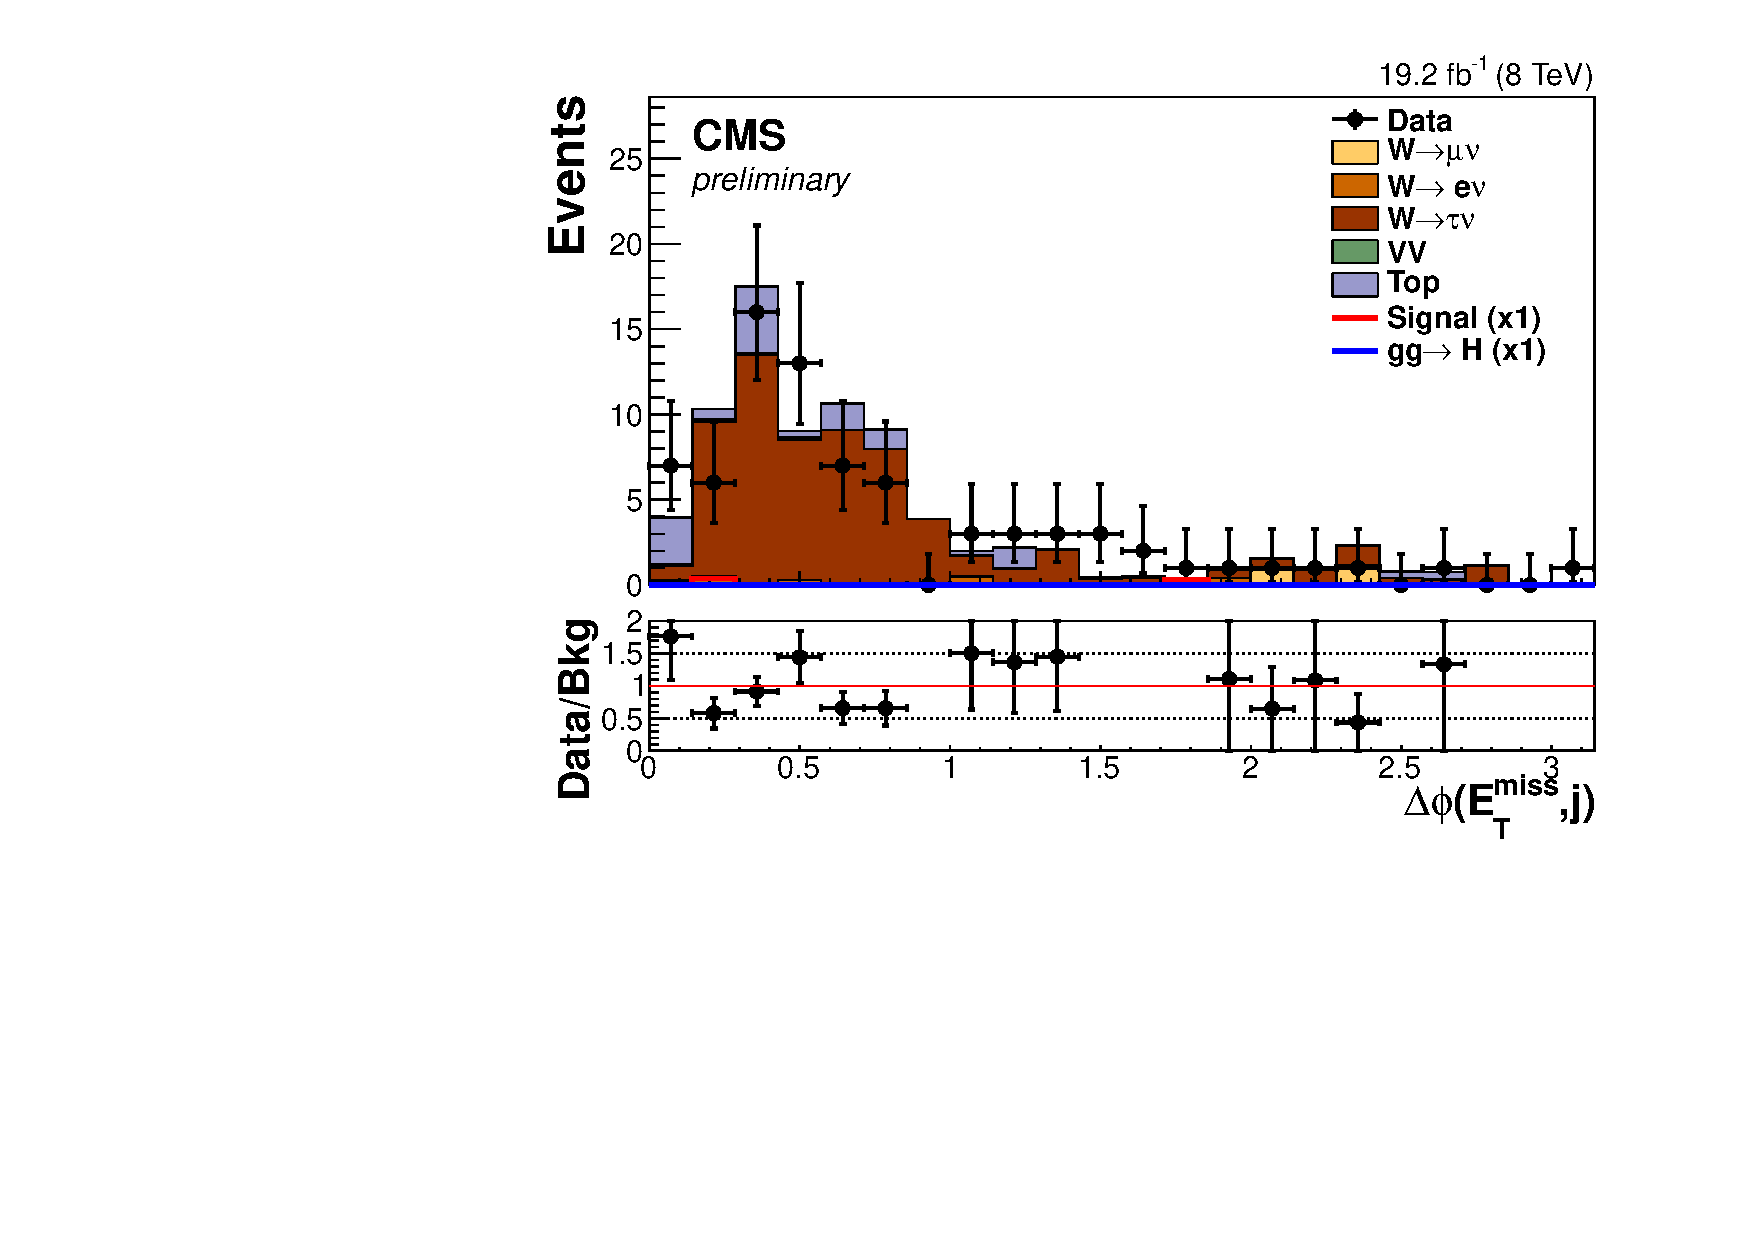
\includegraphics[width=.45\textwidth]{Chapter07/Images/output_sigreg/taunu_alljetsmetnomu_mindphi.pdf}}
\caption{Minimum azimuthal angle separation between any jet with $p_{T}>30$ GeV and the \gls{MET} $\Delta\phi(\text{MET},jets)$ for the (a) $W\rightarrow e\nu$, (b) $W\rightarrow\mu\nu$ and (c) $W\rightarrow\tau\nu$ control regions \cite{ARTICLE:CMSVBFHiggsInvisibleParkedAnalysisPAS}.}
\label{FIGURE:ParkedDataAnalysis_WBackground_MinDeltaPhi}
\end{figure}
 
All presented distribution show good agreement between data and \gls{MC} simulation. The event yields in each control region for both data and \gls{MC} simulation and the final estimations of the W$\rightarrow l\nu$ backgrounds in the signal region can be found in table \ref{TABLE:ParkedDataAnalysis_WBackground_Summary}.
 
\begin{table}[!htb]
\centering
\begin{tabular}{|l|c|c|c|}
\hline
 & W$\rightarrow$e$\nu$ & W$\rightarrow\mu\nu$ & W$\rightarrow\tau\nu$ \\
\hline\hline
$N_{C}^{data}$ &    $68\pm8.2$ &   $300\pm17.3$ &    $76\pm8.7$ \\
$N_{C}^{bkg}$  &   $3.5\pm1.2$ &  $14.8\pm2.5$  &  $13.3\pm2.8$ \\
$N_{C}^{MC}$   & $128.0\pm8.0$ & $399.9\pm14.9$ &  $80.8\pm6.4$ \\
$N_{S}^{MC}$   & $114.9\pm8.9$ & $143.7\pm10.2$ & $121.9\pm8.7$ \\
\hline\hline
SF             & $0.50\pm0.06\pm0.03$ & $0.71\pm0.04\pm0.03$ & $0.78\pm0.11\pm0.07$ \\
\hline\hline
$N_{S}$        & $57.9\pm7.4\pm7.7$ & $102.5\pm6.2\pm11.7$ & $94.6\pm13.1\pm23.8$ \\
\hline
\end{tabular}
\caption{Summary of the W background estimates. The quoted uncertainties are of statistical origin. Systematic uncertainties are shown, as well, for SF and $N_S$. The systematic uncertainty given for SF contains only the \gls{MC} statistics, whereas for $N_{S}$ it represents the full systematic are shown \cite{ARTICLE:CMSVBFHiggsInvisibleParkedAnalysisPAS}.}
\label{TABLE:ParkedDataAnalysis_WBackground_Summary}
\end{table}

The cross check analysis has determined exactly the same data event yields for all W control selection regions further validating the obtained predictions in the signal region.

\clearpage

%%%%%%%%%%%%%%%%%%%%%%%%%%%%%%%%%%%%%%%%%%%%%%%%%%%%%%%%%%%%%%%%%%%%%%%%%%%%%%%%%%%%
%%% SUBSECTION
%%%%%%%%%%%%%%%%%%%%%%%%%%%%%%%%%%%%%%%%%%%%%%%%%%%%%%%%%%%%%%%%%%%%%%%%%%%%%%%%%%%%
\subsection{Top background estimation}
\label{SECTION:ParkedDataAnalysis_ControlRegions_TopBackground}

%Status: DONE (reviewed J.Pela x1)

%TODO: Wrong definition of region 1 in the article
To estimate the contribution of processes involving the top quark in the signal region, two control regions were defined. The first region is the same as the one used for the signal region with the exception that the lepton vetoes are replaced by selecting two tight leptons, exactly one tight electron and one tight muon and no other additional leptons. The $\Delta\phi(\text{MET},jets)$ is not performed to increase statistics.  This region is found to be composed almost entirely of $t\bar{t}$ events. The data event yield in this region was determined to be of 21 events, by both main and cross check analysis. The data-to-simulation scale factor obtained are $1.21\pm 0.19$ (data stat.)$ \pm 0.16 $(syst.).

%TODO: Not in the analysis note, how was this combined into the final result?
A second region selects events with same criteria as the signal region with the exception that the lepton vetoes are replaced by selecting a single tight lepton (e or $\mu$) and no other additional leptons. Additionally, one of the leading jets is required to be identified as a jet from a b quark (using the Combined Secondary Vertex algorithm \cite{ARTICLE:CMSIdentificationOfbQuarks}). The composition of this region was determined to be with the help of \gls{MC} simulation 10\% single top, 50\% $t\bar{t}$ and 40\% W+jets. For this region the main analysis observed 429 events which lead to a data-to-simulation scale factor of $0.88\pm 0.07$ (data stat.)$ \pm 0.08$ (syst.). The systematics uncertainties associated with the determined scale factors are dominated by the small statistics available in \gls{MC} simulation. Taking into account these results a 20\% systematic uncertainty is assigned to the top quark contribution to the signal region. 

%%%%%%%%%%%%%%%%%%%%%%%%%%%%%%%%%%%%%%%%%%%%%%%%%%%%%%%%%%%%%%%%%%%%%%%%%%%%%%%%%%%%
%%% SUBSECTION
%%%%%%%%%%%%%%%%%%%%%%%%%%%%%%%%%%%%%%%%%%%%%%%%%%%%%%%%%%%%%%%%%%%%%%%%%%%%%%%%%%%%
\subsection{QCD background estimation}
\label{SECTION:ParkedDataAnalysis_ControlRegions_QCDBackground}

%Status: DONE (reviewed J.Pela x1)

%TODO: What shape?
The contribution of \gls{QCD} multi-jet processes is determined with a data driven method using non-isolated \gls{MET}. Three regions are defined: Region I is denoted as ``inverted'' and gives the description of the \gls{QCD} multi-jet shape; Region II is denoted as ``3-jet'' where a cross check is preformed to see how well the \gls{QCD} multi-jet shapes are described; and Region III is denoted as ``sideband'' in this region the normalization of the \gls{QCD} multi-jet shapes is extracted to apply to the signal region.

% QCD Shape region
The \gls{QCD} multi-jet \textit{inverted region}, is selected by changing the $\Delta\phi(\text{MET},jets)$ requirement to $min(\Delta\phi(\text{MET}),jets)<1.0$ while requiring $\Delta\phi(\text{MET},jet_{1,2})>2.3$. The change in requirements provides two leading jets which are signal like, but at the same time ensures \gls{MET} will not be isolated. The distribution of $\text{MET}_{sig}$ after in the inverted region is shown in figure \ref{FIGURE:ParkedDataAnalysis_QCDBackground_Plots}. The selected events in this region are expected to originate about 20\% from W, Z and top processes. The \gls{QCD} shape is defined as the shape observed in data after the subtraction of non-\gls{QCD} backgrounds which are normalised by scale factors determined in their respective control regions but with the same inverted selection. Good agreement between data and the \gls{VBF} enriched \gls{QCD} \gls{MC} simulation in this region is observed as shown in figure \ref{FIGURE:ParkedDataAnalysis_QCDBackground_Plots}.

% TODO: NOT IN THE AN!!! is it norm 3?
The \textit{3-jet region} is defined by requiring $\Delta\phi(\text{MET},jets)>1.0$, $\text{MET}_{sig}>3$ and at least three jets with p$_{T}>30\,\GeV$. Using \gls{MC} simulation the contribution from signal to this region was determined to be negligible. This region is used to ensure that the \gls{QCD} shape is adequate. The expected number of \gls{QCD} events in the \textit{3-jet region}, n$_{QCD}^{3j}$, is the data yield in this region subtracted from backgrounds with the W and Z predictions being normalised to their control leptonic regions. The \gls{QCD} shape can now be compared between the data in this region and the \textit{inverted region} with $\Delta\phi(\text{MET},jet_{1,2})>1.0$ and normalizing it to n$_{QCD}^{3j}$. The distribution of $\text{MET}_{sig}$ in the \textit{3-jet region} is shown in figure \ref{FIGURE:ParkedDataAnalysis_QCDBackground_Plots}. The discrepancy between data and the prediction is found to be less than 20\%. unfortunately, since most of the events in the signal region will only have two jets, this control region cannot be used for the final \gls{QCD} multi-jet estimation.

\begin{figure}[!htb]
\centering
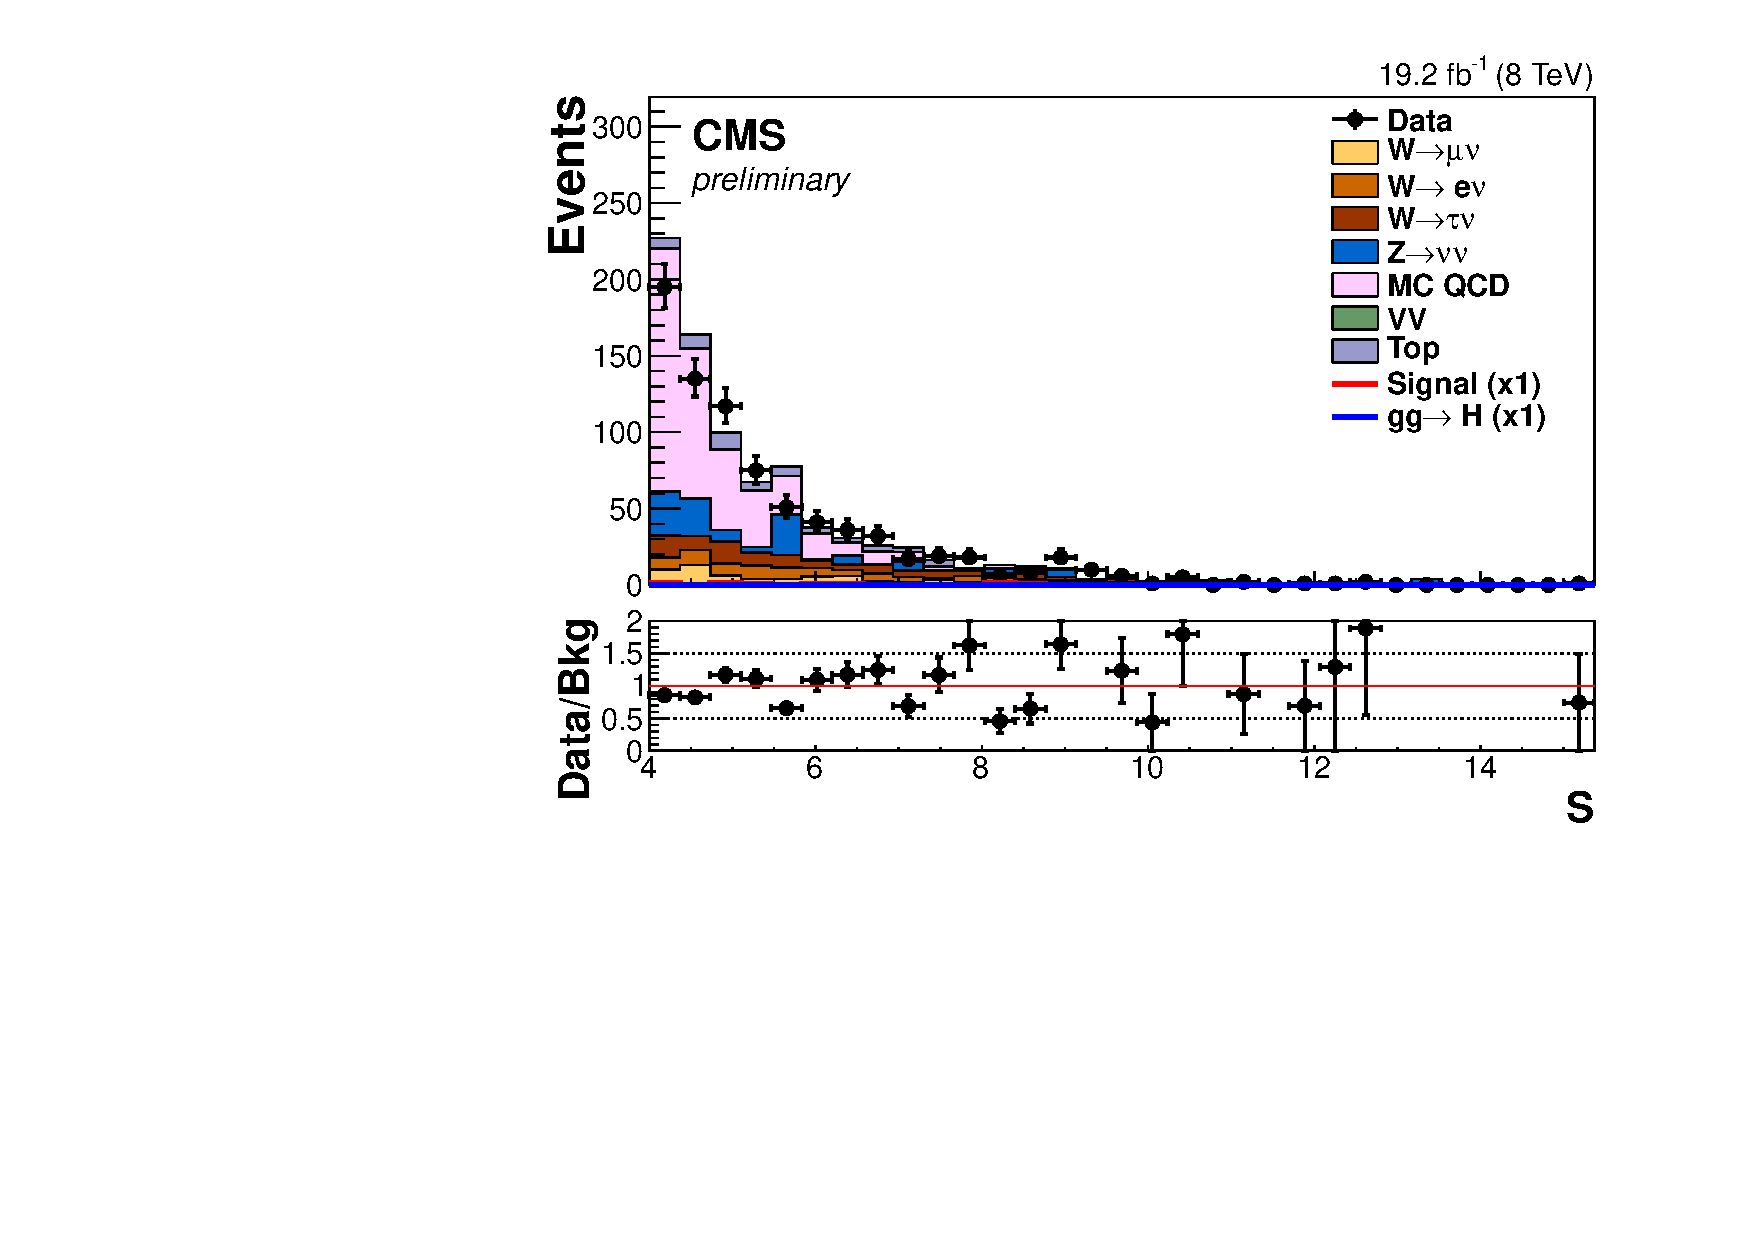
\includegraphics[width=.45\textwidth]{Chapter07/Images/output_invqcd_qcd_metnomu_significance.pdf}
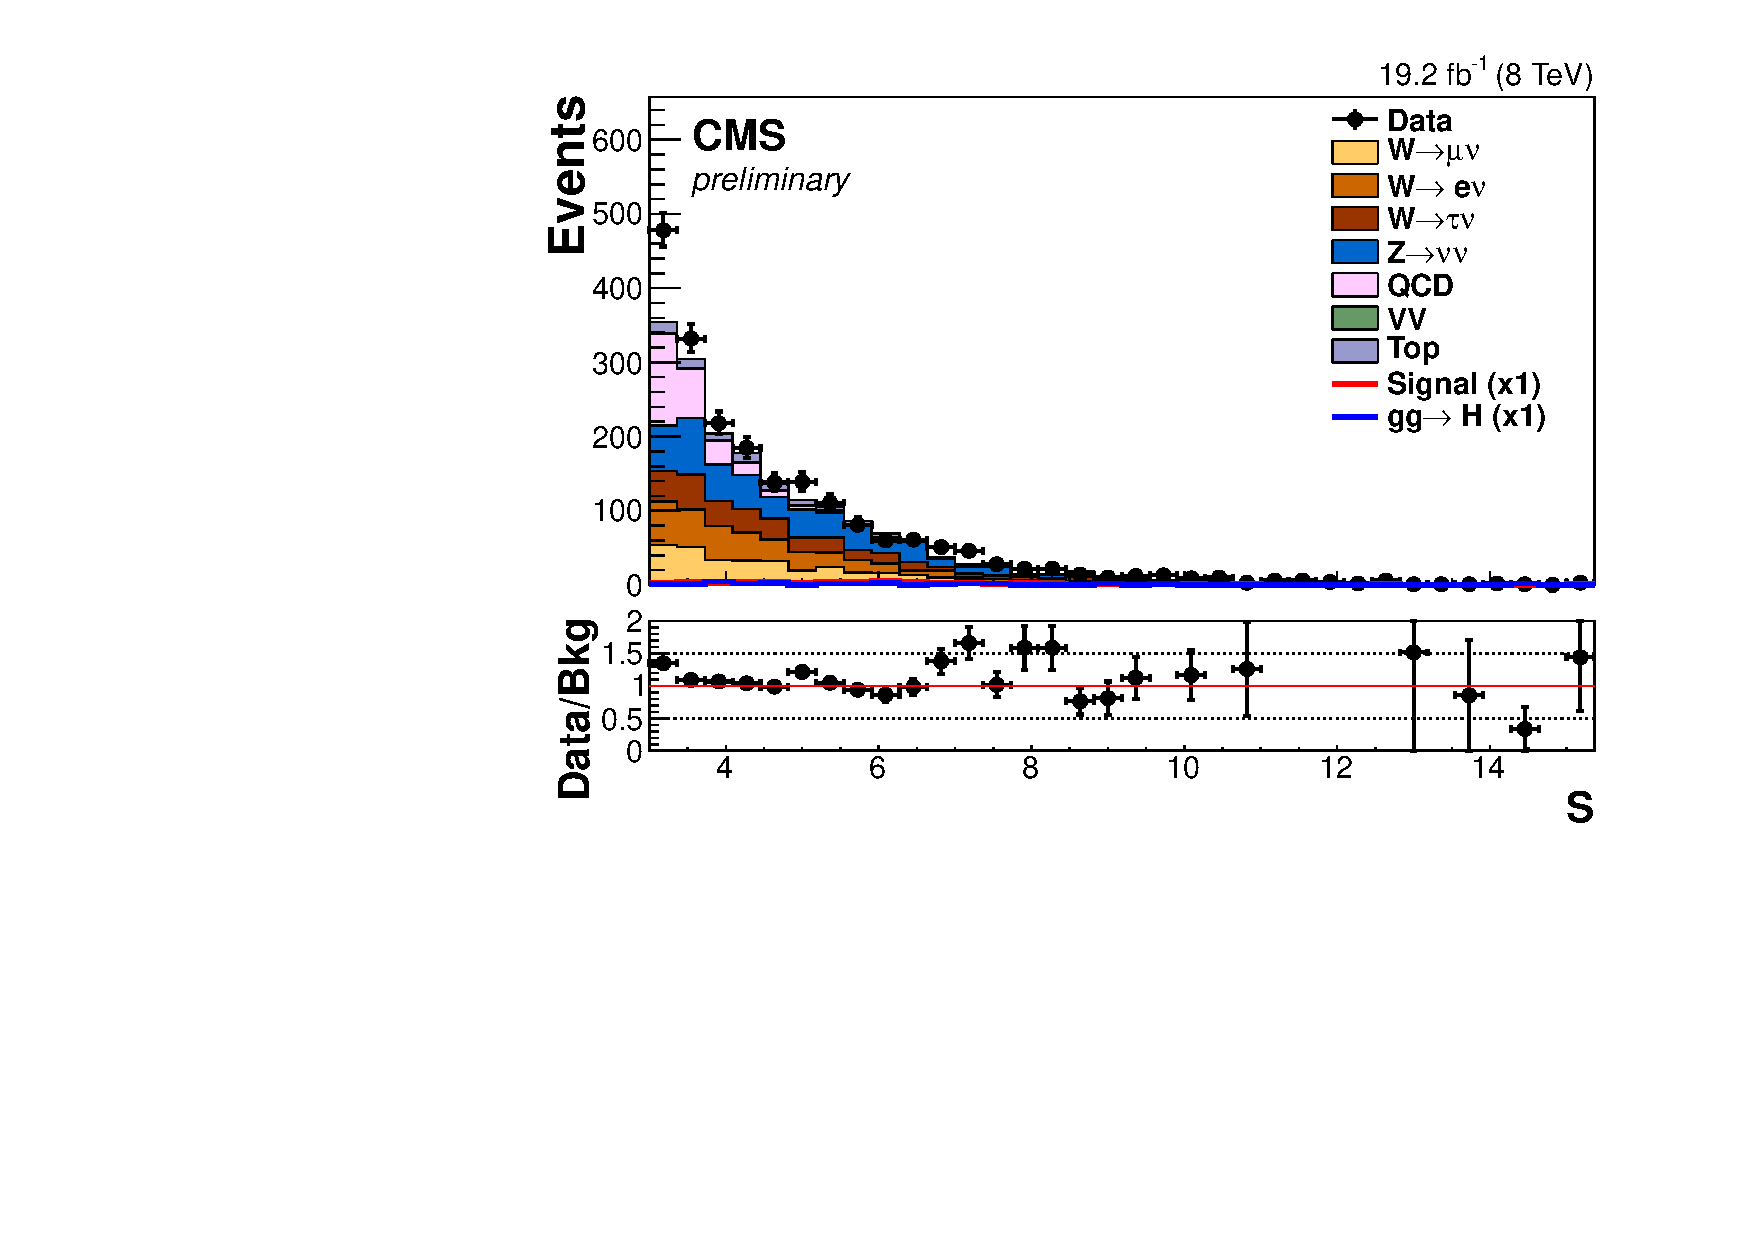
\includegraphics[width=.45\textwidth]{Chapter07/Images/output_invqcd_3j_nunu_metnomu_significance.pdf}
\caption{(left) \MET significance $\text{MET}_{sig}$ for events with $\Delta\phi(\text{MET},jets)<1.0$ and $\Delta\phi(\text{MET},jet_{1,2})>2.3$. MC QCD is the \gls{QCD} \gls{MC} normalised to the background-subtracted data yield. (right) \gls{MET} significance, $\text{MET}_{sig}$, for events with $\Delta\phi(\text{MET},jets)>1.0$ and at least 3 jets with $p_T>30\,\GeV$. The \gls{QCD} is modelled by data using the inverted $\Delta\phi(\text{MET},jets)<1.0$ and $\Delta\phi(\text{MET},jet_{1,2})>1$ selection, after background subtraction, and normalised to the background-subtracted data yield. In both figures, the W and Z backgrounds have been normalised to their respective control regions in the same conditions. The last bin represents all those events falling above the range of the histogram \cite{ARTICLE:CMSVBFHiggsInvisibleParkedAnalysisPAS}.}
\label{FIGURE:ParkedDataAnalysis_QCDBackground_Plots}
\end{figure}

% NORM 1 
%TODO: What happens to the all mindeltaphi cut??? Is it extrapolated shape????
The \textit{sideband region} is used to determine the normalization of the \gls{QCD} shape to be used in the signal region. This region is defined by selecting events with $3<\text{MET}_{sig}<4$ and $1.0<\Delta\phi(\text{MET},jet_{1,2})<2.0$. In this region it is observed that the normalisation factor decreases rapidly with increasing requirements as a function of $\text{MET}_{sig}$ and as a function of $\Delta\phi(\text{MET},jet_{1,2})$. This normalization factor variation is fitted and extrapolated to the signal region requirements. The average of the two extrapolation factors is used as the central prediction and the envelope is used to assign the systematic uncertainty on the \gls{QCD} multi-jets normalisation.

%%%%%%%%%%%%%%%%%%%%%%%%%%%%%%%%%%%%%%%%%%%%%%%%%%%%%%%%%%%%%%%%%%%%%%%%%%%%%%%%%%%%
%%% SECTION
%%%%%%%%%%%%%%%%%%%%%%%%%%%%%%%%%%%%%%%%%%%%%%%%%%%%%%%%%%%%%%%%%%%%%%%%%%%%%%%%%%%%
\section{Systematics}

%Status: DONE (reviewed J.Pela x1)

The dominant source of uncertainty is due to the statistical uncertainty associated with the yields of the control regions both in data and \gls{MC} simulation, which are used for the estimation of the different backgrounds in signal region. 

The errors associated to the jet energy scale, unclustered energy scale and jet energy resolution are estimated for both signal and background processes by varying each quantity independently by its uncertainties \cite{ARTICLE:CMSDeterminationJetEnergyCalibration}. For each variation the \gls{MET} is recomputed and the signal and backgrounds predictions are recalculated. A similar procedure is applied for the lepton efficiency and \gls{PU} scale factors which are applied to the \gls{MC} simulation, which are also varied by their uncertainties and propagated through the analysis \cite{ARTICLE:CMSMuonReconstruction7TeV,ARTICLE:CMSElectronReconstruction8TeV}.

The uncertainty associated with the integrated luminosity measurement is of 2.6\% and is only applied to the \gls{MC} simulated signal and backgrounds \cite{ARTICLE:CMSLuminosityBasedonPixelClusterCounting}. The main backgrounds are normalised using a data-driven method which takes into account the trigger efficiency, while the impact of the luminosity measurement in the signal and minor backgrounds was found to be negligible.

Uncertainties associated with diboson cross sections are taken from \gls{CMS} measurements \cite{ARTICLE:CMSMeasurmentOfWWandZZxsec}, while the theoretical uncertainties due to \gls{PDF} and \gls{QCD} scales associated to the signal cross section are taken from the \gls{LHC} Higgs Cross Section Working Groups Yellow Report 3 \cite{ARTICLE:HandbookofLHCHiggsCrossSectionsInclusiveObservables,ARTICLE:HandbookofLHCHiggsCrossSectionsDifferentialDistributions}.

% TODO: Ask patrick, ``compatible within statistical uncertainty`` of what?
The uncertainty of the extrapolation of the  $Z\rightarrow\nu\nu$ background obtained from the \gls{QCD} production of $Z/\gamma^{*}\rightarrow\mu\mu$ was estimated by comparing the prediction from \textsc{MADGRAPH} and a\textsc{MC@NLO\_MG5} \cite{ARTICLE:aMCatNLO}. The results from both generators were compatible within statistical uncertainty, leading to no additional uncertainties being added. 

Table \ref{TABLE:ParkedDataAnalysis_Systematics_Summary} shows a summary of the overall size of each uncertainty as a percentage of the total signal and background predictions.

\begin{table}[!htb]
\centering
\begin{tabular}{|l|c|c|}
\hline 
Source                                            & Total background &     Signal \\
\hline\hline
Control region data stat.                          &            9.3  &          - \\
MC stat.                                           &            5.4  &        3.8 \\
Jet energy scale                                   &            4.6  &         11 \\
$W\rightarrow\tau\nu$ control region extrapolation &            4.3  &          - \\
QCD normalisation                                  &            3.2  &          - \\
Jet energy resolution                              &            3.0  &        1.8 \\
Lepton ID efficiency                               &            2.4  &          - \\
Unclustered energy scale                           &            1.9  &        1.6 \\
Pileup weight                                      &            1.1  &        1.5 \\
Top MC scale factor unc.                           &            0.25 &          - \\
Luminosity                                         &            0.02 &        2.6 \\
QCD scale, PDF and cross section uncertainties     &            0.01 &        5.2 \\
\hline
\end{tabular}
\caption{Summary of the uncertainties on the total background and signal yields. All uncertainties affect the normalization of the yield, and are quoted as the change in \% in the total background or signal estimate, when each systematic effect is varied according to its uncertainties. The signal uncertainties are given for $m_H=125$\GeV and $\BRinv=100$\%. \cite{ARTICLE:CMSVBFHiggsInvisibleParkedAnalysisPAS}}
\label{TABLE:ParkedDataAnalysis_Systematics_Summary}
\end{table}

%%%%%%%%%%%%%%%%%%%%%%%%%%%%%%%%%%%%%%%%%%%%%%%%%%%%%%%%%%%%%%%%%%%%%%%%%%%%%%%%%%%%
%%% SECTION
%%%%%%%%%%%%%%%%%%%%%%%%%%%%%%%%%%%%%%%%%%%%%%%%%%%%%%%%%%%%%%%%%%%%%%%%%%%%%%%%%%%%
\section{Results}

%Status: DONE (reviewed J.Pela x1)

The final estimations of the number of events predicted in the signal region are estimated from \gls{MC} simulation for the W, Z, or with the use of non-isolated \gls{MET} events in the case of the \gls{QCD} multi-jet background, with normalizations obtained from control regions. The remaining backgrounds are estimated directly from \gls{MC} simulation. These results are summarized in table \ref{TABLE:ParkedDataAnalysis_Results_Summary}.

% New numbers cross check
% Wrong? Signal Region - Top     : 5.02825+/-1.21163
% Wrong? Signal Region - VV      : total: 3.5+/-0.5  ZZ: 0.717446 +/- 0.153554 WW: 0.68089 +/- 0.249246 WZ: 2.13829 +/- 0.365195
% Wrong? Signal Region - Sig VBF : 267.7 +/- 9.1 (stat) 
% Wrong? Signal Region - Sig ggH :  21.7 +/- 6.0 (stat) 

% Region Zmumu  - Data       : 18 +/- 4.24264 (stat) 
% Region Zmumu  - Z total    : 16.1181 +/- 1.85029 (stat)  100.0%
% Region Zmumu  - Z QCD      : 11.1848 +/- 1.84217 (stat)   69.3%
% Region Zmumu  - Z EWK      : 4.93329 +/- 0.173201 (stat)  30.6%
% Region Zmumu  - VV         : 0.141569 +/- 0.103953 (stat) 
% Region Zmumu  - Top        : 0 +/- 0
% Region Zmumu  - W          : 0 +/- 0
% Region Zmumu  - QCD        : 0 +/- 0
% Region Zmumu  - QCD VBF    : 0 +/- 0
% Region Signal - XSec Ratio : 5.651 +/- 0.023 = B
% Region Signal - Eff  Ratio : (1.8 +/- 0.1)x10e-6 / (1.2 +/- 0.1)x10e-6 = 1.5 +/- 0.15 = A 
% Region Signal - Z in CR    : N_data - N_bkg = 17.86 +/- 4.2439133 = N
% Region Signal - Prediction : N * A * B = 151.38 +/- 39.0

% Region Elec+MET - Data    : 68 +/- 8.24621      
% Region Elec+MET - W total : 87.9693 +/- 7.69928 : 
% Region Elec+MET - W elec  : 87.249 +/- 7.68202  : W decay 1293.81 +/- 25.388
% Region Elec+MET - W muon  : 14.3927 +/- 2.87926 : W decay 148.326 +/- 8.42063
% Region Elec+MET - W muon  : 15.0921 +/- 2.92494 : W decay 151.568 +/- 8.51961

\begin{table}[!htb]
\centering
\begin{tabular}{|l|c|}
\hline 
Process & Event yields \\
\hline\hline
$Z\rightarrow\nu\nu$  & $158.1 \pm 37.3 \pm 21.2$ \\
$W\rightarrow\mu\nu$  & $102.5 \pm 6.2  \pm 11.7$ \\
$W\rightarrow e\nu$   & $ 57.9 \pm 7.4  \pm  7.7$ \\
$W\rightarrow\tau\nu$ & $ 94.6 \pm 13.1 \pm 23.8$ \\
top                   & $  5.5 \pm 1.8$           \\ 
VV                    & $  3.9 \pm 0.7$           \\ 
QCD multijet          & $   17 \pm 14$            \\
\hline\hline
Total Background      & $439.4 \pm 40.7 \pm 43.5$ \\
\hline\hline
Signal(VBF)           & $273.1 \pm 31.2 $         \\   
Signal(ggH)           & $ 23.1 \pm 15.9 $         \\   
\hline\hline
Observed data         & 508                       \\
\hline
\end{tabular}
\caption{Summary of the estimated number of background and signal events, together with the observed yield, in the \gls{VBF} search signal region. The signal yield is given for $m_H=125$\GeV and $\BRinv=100$\%. Where two errors quoted they are the statistical and systematic uncertainties respectively, where only one is quoted it is the systematic uncertainty \cite{ARTICLE:CMSVBFHiggsInvisibleParkedAnalysisPAS}.}
\label{TABLE:ParkedDataAnalysis_Results_Summary}
\end{table}

Distributions of the $\Delta\eta_{jj}$, $M_{jj}$, $\text{MET}_{sig}$ and \gls{MET} variables, in the signal region, are shown in figure \ref{FIGURE:ParkedDataAnalysis_Results_SigRegPlots}. 

\begin{figure}[!htb]
\centering
\subfloat[]{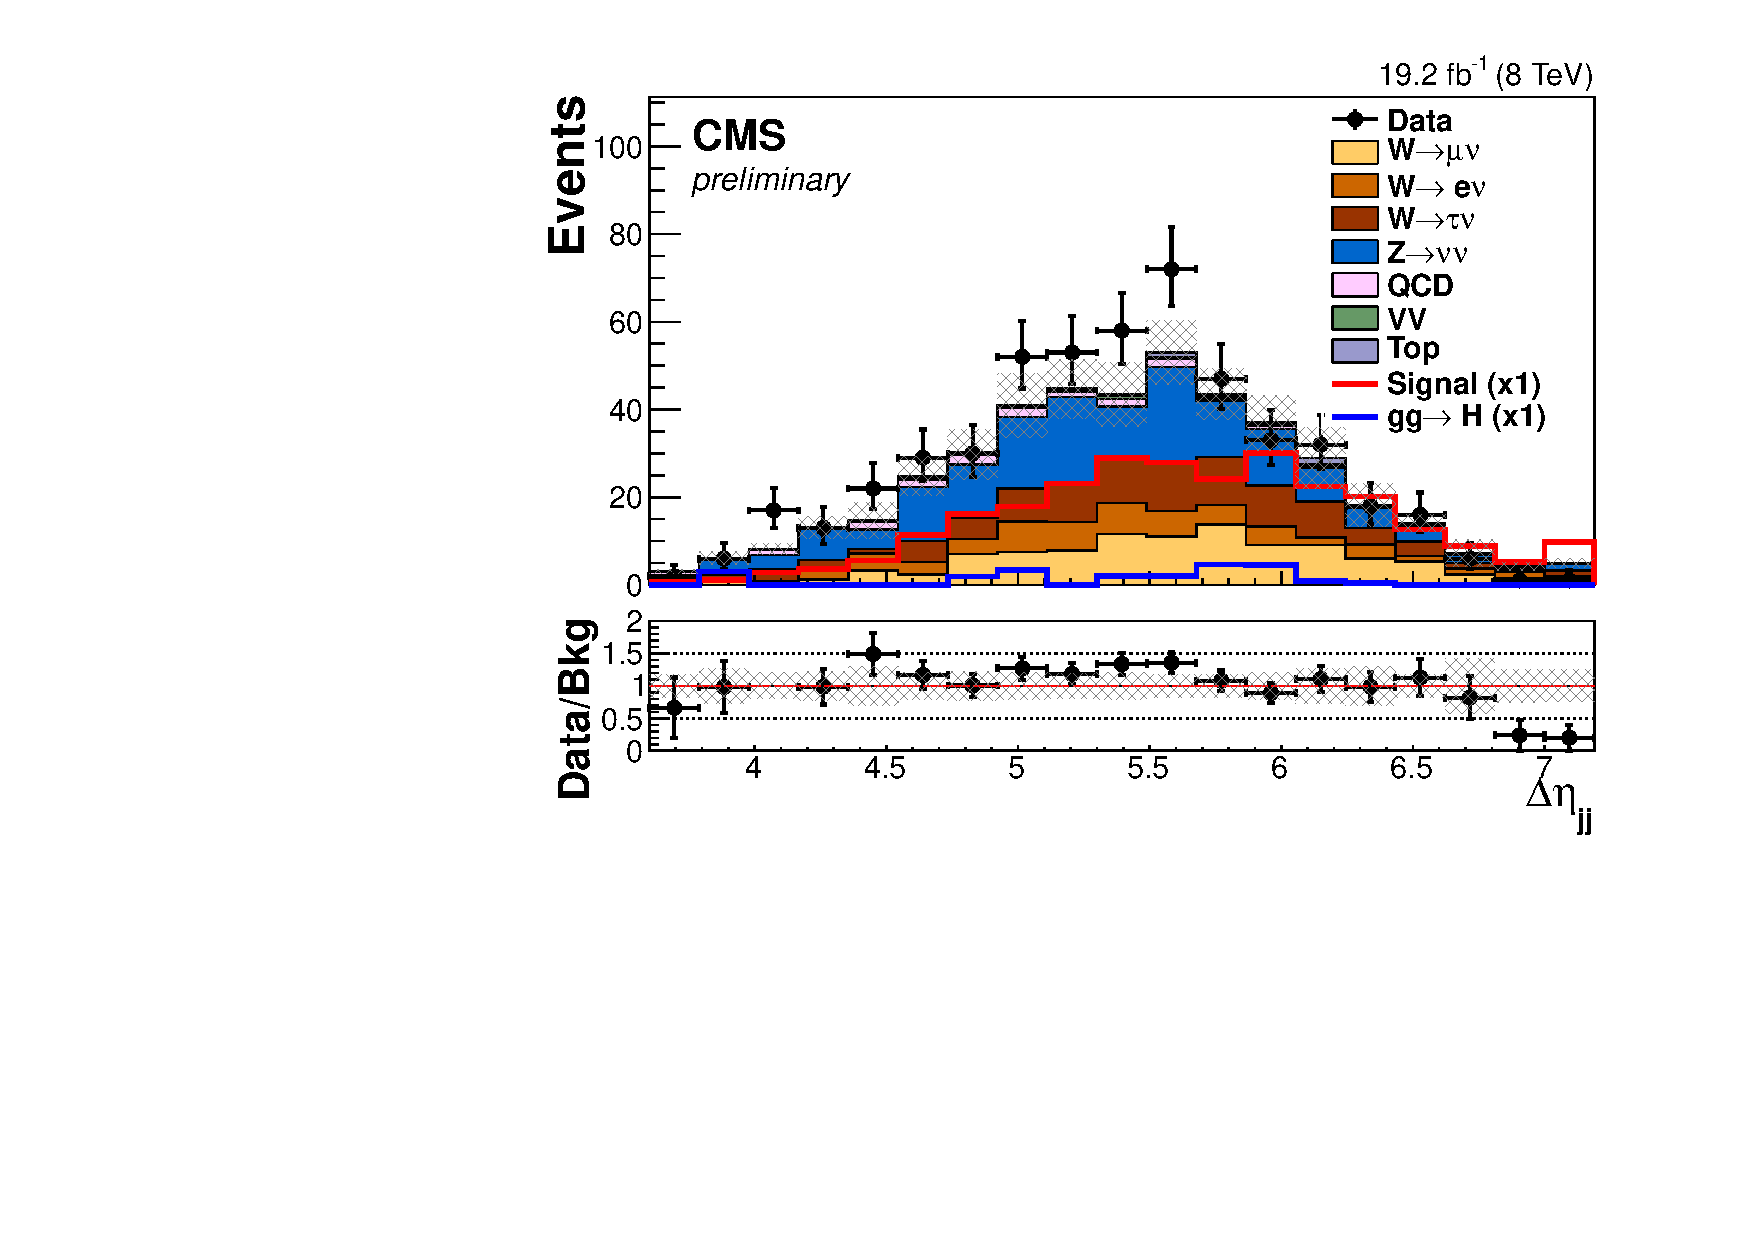
\includegraphics[width=.45\textwidth]{Chapter07/Images/output_sigreg/nunu_dijet_deta.pdf}}
\subfloat[]{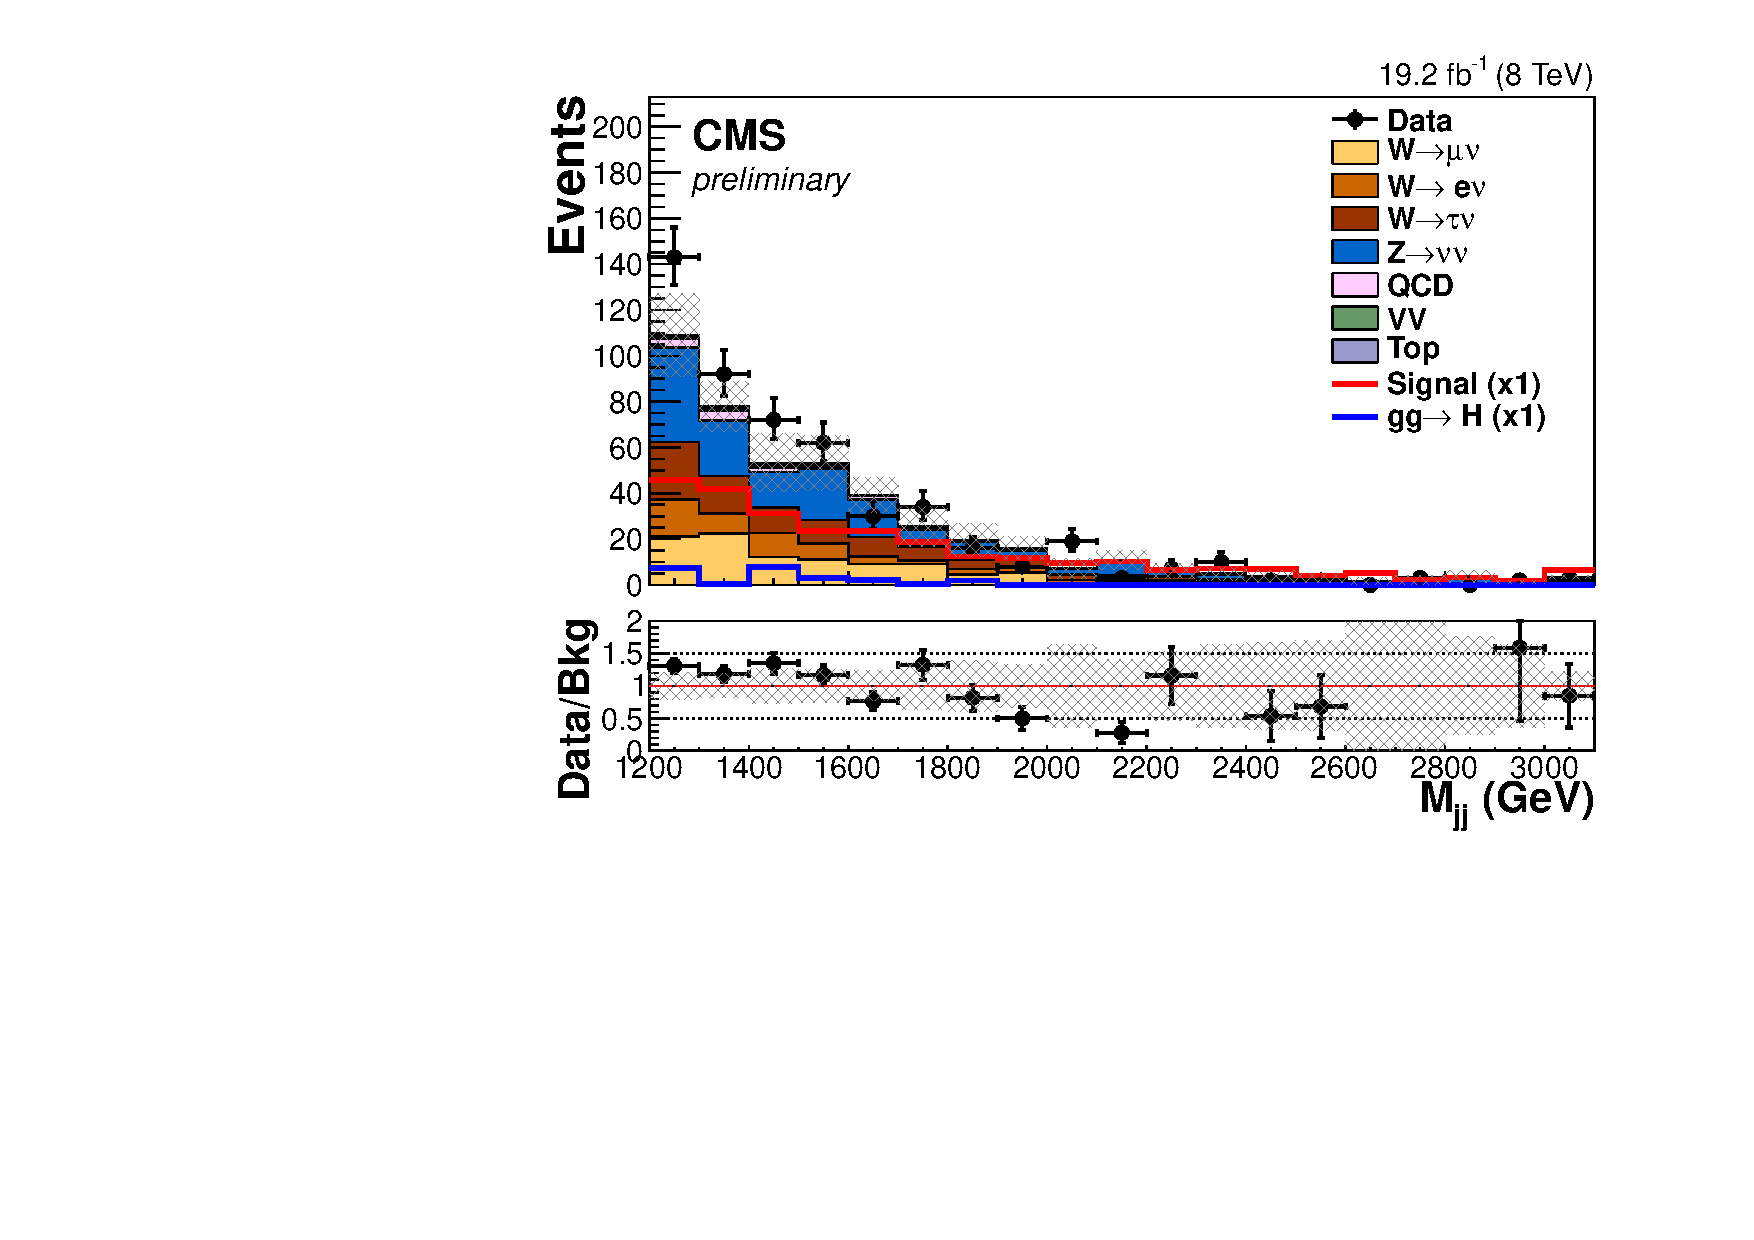
\includegraphics[width=.45\textwidth]{Chapter07/Images/output_sigreg/nunu_dijet_M.pdf}} \\
\subfloat[]{\includegraphics[width=.45\textwidth]{Chapter07/Images/output_sigreg/nunu_metnomu_significance.pdf}}
\subfloat[]{\includegraphics[width=.45\textwidth]{Chapter07/Images/output_sigreg/nunu_metnomuons.pdf}}
\caption{(a) Pseudorapidity difference between the two selected \gls{VBF} jets $\Delta\eta_{jj}$, (b) dijet mass $M_{jj}$, (c) \gls{MET} significance $\text{MET}_{sig}$; and (d) \gls{MET}, in the signal region. The last bin represents all those events falling above the range of the histogram. An excess is seen which is less than 2$\sigma$ in significance as can be observed from the hatched band which indicates the size of the total uncertainty on the background estimate \cite{ARTICLE:CMSVBFHiggsInvisibleParkedAnalysisPAS}.}
\label{FIGURE:ParkedDataAnalysis_Results_SigRegPlots}
\end{figure}

\clearpage

%%%%%%%%%%%%%%%%%%%%%%%%%%%%%%%%%%%%%%%%%%%%%%%%%%%%%%%%%%%%%%%%%%%%%%%%%%%%%%%%%%%%
%%% SUBSECTION
%%%%%%%%%%%%%%%%%%%%%%%%%%%%%%%%%%%%%%%%%%%%%%%%%%%%%%%%%%%%%%%%%%%%%%%%%%%%%%%%%%%%
\subsection{Comparison with the cross-check analysis}

%Status: DONE (reviewed J.Pela x1)

The cross check analysis has successfully validated the main analysis by reproducing the data event yields in all the relevant regions. All event yields were measured to be exactly the same in both analysis except the yield in the \gls{QCD} sideband region where a discrepancy of +1.1\% was observed. Since the \gls{QCD} multi-jet background is a minor background, representing less than 4\% of the total background, this level of synchronization was deemed acceptable. Table \ref{TABLE:ParkedDataAnalysis_Results_MainCrossCheckComparison} shows a comparison of the event yield obtained by both analysis and the fractional difference for each region.

\begin{table}[!htb]
\centering
\begin{tabular}{|l|c|c|c|}
\hline
Region                & Main & Cross Check & Difference [\%] \\
\hline\hline
$Z\rightarrow\nu\nu$  &   18 &          18 &             0.0 \\
$W\rightarrow\mu\nu$  &  300 &         300 &             0.0 \\
$W\rightarrow e\nu$   &   68 &          68 &             0.0 \\
$W\rightarrow\tau\nu$ &   76 &          76 &             0.0 \\
top (Region 1)        &   21 &          21 &             0.0 \\
QCD Sideband region   & 1586 &        1603 &            +1.1 \\
% QCD Region II         &  411 &         412 &            +0.2 \\
% QCD Norm3             & 1517 &        1523 &            +0.4 \\
\hline\hline
Signal                &  508 &         508 &             0.0 \\
\hline
\end{tabular}
\caption{Comparison of the data event yields in all relevant regions, between the main and cross check analyses. The column ''Difference`` is defined a $(N_{\text{Cross Check}}-N_{\text{main}})/N_{\text{main}}$.}
\label{TABLE:ParkedDataAnalysis_Results_MainCrossCheckComparison}
\end{table}

%%%%%%%%%%%%%%%%%%%%%%%%%%%%%%%%%%%%%%%%%%%%%%%%%%%%%%%%%%%%%%%%%%%%%%%%%%%%%%%%%%%%
%%% SECTION
%%%%%%%%%%%%%%%%%%%%%%%%%%%%%%%%%%%%%%%%%%%%%%%%%%%%%%%%%%%%%%%%%%%%%%%%%%%%%%%%%%%%
\section{Limits on the cross section of invisibly decaying Higgs bosons}
\label{SECTION:ParkedDataAnalysis_Limits}

%Status: DONE (reviewed J.Pela x1)

As shown in table \ref{TABLE:PromptDataAnalysis_BackgroundEstimation_BackgroundSummary}, 508 data events were observed in the signal region, this yield is compatible with the background only prediction. Since no evidence of signal is observed 95\% \gls{CL} upper limits on the Higgs boson production cross section times branching fraction are computed. The limits are calculated using the asymptotic $\mathrm{CL}_\mathrm{s}$ method \cite{ARTICLE:CLsTechnique,ARTICLE:CLCompForCombiningSearchesWithSmallStat,ARTICLE:HandbookofLHCHiggsCrossSectionsDifferentialDistributions} based on asymptotic formulae \cite{ARTICLE:AsymptoticCLS}, following the standard \gls{CMS} Higgs boson searches combination technique \cite{ARTICLE:CMS_HiggsDiscovery,ARTICLE:HiggsCombination}. Systematic uncertainties are incorporated as nuisance parameters and treated according to the frequentist paradigm \cite{ARTICLE:HiggsCombination} and all correlations between processes are taken into account.

If \gls{SM} production cross sections and acceptances are assumed, the observed (expected) 95\% C.L. limit on \BRinv\, of a \gls{SM} $125\,\GeV$ Higgs boson is 57\% (40\%). Figure \ref{FIGURE:ParkedDataAnalysis_Limits_VBFLimit} shows the the 95\% C.L. limit on \BRinv and the 95\% C.L. limit on the cross section times \BRinv\,, both under the assumption of \gls{SM} Higgs boson acceptances as a function of Higgs mass.

\begin{figure}[!htb]
\centering
\includegraphics[width=0.49\textwidth]{Chapter07/Images/vbflimit.pdf}
\includegraphics[width=0.49\textwidth]{Chapter07/Images/vbfxslimit.pdf}
\caption{The 95\% C.L. limit on \BRinv\, of a SM Higgs boson (left) and the 95\% C.L. limit on the cross section times \BRinv\ (right) as a function of the Higgs boson mass, assuming SM Higgs boson acceptances \cite{ARTICLE:CMSVBFHiggsInvisibleParkedAnalysisPAS}.}
\label{FIGURE:ParkedDataAnalysis_Limits_VBFLimit}
\end{figure}

AS it can be observed in table \ref{TABLE:ParkedDataAnalysis_Systematics_Summary}, similarly to the \textit{prompt analysis} the dominant source of systematic uncertainty is the limited number of events present in the control regions both in data and \gls{MC} simulation. This effect is particularly noticeable in the Z control region, if this region statistical uncertainty was of the order of the one measured in the $W\rightarrow\mu\nu$ control region the expected 95\% C.L. limit on the cross section times \BRinv for a \gls{SM} 125 GeV Higgs boson would be reduced to 33\%.

%TODO: Should I write the combined stuff???
% The result is also combined with that obtained by CMS in searches in the channel where the Higgs boson is produced in association with a Z which was reported in ~\cite{Chatrchyan:2014tja}. The procedure for this combination is also described in ~\cite{Chatrchyan:2014tja}. The 95\% C.L. observed (expected) limit on \BRinv\, after combination is 47\% (35\%) for a SM 125 GeV Higgs boson.

  \chapter{Run II Preparation}
\label{CHAPTER:RunIIPreparation}

\glsresetall % Resetting all acronyms

%Status: DONE

After the successful completion of the the first data taking period, the \gls{LHC} Run I, the accelerator and detectors went through a two year long technical shut-down which was designated the \gls{LS1}. During the period the accelerator completed a consolidation and improvement program to allow a ramp up of the beams energy up to the design value of $7\,\TeV$ per beam in proton-proton mode. At the same time the experiments also performed maintenance, repair and improvement programs. 

Data analysis continued during this period of no data taking using the datasets already available or the newly reconstructed parked data. After this final work over $8\,\TeV$ data was completed most \gls{CMS} physics analysis started their preparation for the \gls{LHC} Run II, where higher collision energies, even higher values of \gls{PU} and more recorded integrated luminosity are expected. Following this global effort the \gls{CMS} \gls{VBF} Higgs to invisible analysis also started its own preparation work. 

The first step is always the definition of a trigger condition for data taking. The effort made to create and study such an adequate set of trigger for the use of this analysis during run II is documented in section \ref{SECTION:RunIITriggerStudies}. Additionally, work was made to study and propose the creation of a dedicated \gls{QCD} \gls{MC} sample with signal like characteristics expanding on the one already created for Run I. This study can be found in section \ref{SECTION:RunIIPreparation_RunIIQCDMonteCarloSamples}.

%%%%%%%%%%%%%%%%%%%%%%%%%%%%%%%%%%%%%%%%%%%%%%%%%%%%%%%%%%%%%%%%%%%%%%%%%%%%%%%%%%%%%%%
%%% SECTION
%%%%%%%%%%%%%%%%%%%%%%%%%%%%%%%%%%%%%%%%%%%%%%%%%%%%%%%%%%%%%%%%%%%%%%%%%%%%%%%%%%%%%%%
\section{Run II trigger studies}
\label{SECTION:RunIITriggerStudies}

% Working areas
% 
% /vols/cms02/jca10/work/slc6/dev01/CMSSW_7_2_0_pre8/src
% /vols/cms02/jca10/work/slc6/dev01/testPhD/CMSSW_7_2_0_pre8/src
%
% Oct 21  2014 jobs
% Oct 14  2014 jobsHLT
% Oct 22  2014 jobsHLTv2
% Oct 22  2014 jobsL1Tv2

% Oct 26  2014 VBFHiggsToInvisible/TriggerStudies/HLT_Run2015
% Oct 26  2014 VBFHiggsToInvisible/TriggerStudies/HLT_Run2015_DijetVBF-ETM50_NOTPFMET170
% Oct 27  2014 VBFHiggsToInvisible/TriggerStudies/HLT_Run2015_ETM70
% Oct 27  2014 VBFHiggsToInvisible/TriggerStudies/HLT_Run2015_ETM70_NOTPFMET170
% Oct 27  2014 VBFHiggsToInvisible/TriggerStudies/L1TAddRate

% Additional rates study: 
% /vols/cms02/jca10/work/slc6/dev01/CMSSW_7_2_0/src/VBFHiggsToInvisible/

%Status: DONE

The first step of any \gls{CMS} physics analysis is to define which trigger to use for data taking. The \gls{TSG} develops generic usage trigger conditions, know as trigger paths, which can be used by any analysis. Typically this conditions cover all possible single objects (single electron, single jets, etc), multiple objects (double electron, triple muon, etc), cross triggers (single electron $+$ sigle muon, etc). In some cases, like for our analysis, it with better to define a custom condition to obtain maximum physics content. The following reasons drove the decision to create a set dedicated trigger paths.

\begin{itemize}
  \item Maximize signal collection efficiency by selecting our signal topology with reduced trigger cuts while compared with generic triggers;
  \item Use again a trigger condition with $MET_{\text{no muon}}$ instead of $MET$ to study \gls{EWK} Z irreducible background;
  \item Create a new dedicate pre-scaled trigger path with reduced thresholds with objective of reducing systematics;
\end{itemize}

For the proposal of our triggers it was decided to produce numbers for a low and high rate scenarios in terms of available \gls{HLT} bandwidth. For the signal trigger path rates $1.5\,\hertz$ and $5.0\,\hertz$ were considered. While for the systematics paths rate $0.1\,\hertz$ and $0.1\,\hertz$ were considered.

%%%%%%%%%%%%%%%%%%%%%%%%%%%%%%%%%%%%%%%%%%%%%%%%%%%%%%%%%%%%%%%%%%%%%%%%%%%%%%%%%%%%%%%
%%% SUBSECTION
%%%%%%%%%%%%%%%%%%%%%%%%%%%%%%%%%%%%%%%%%%%%%%%%%%%%%%%%%%%%%%%%%%%%%%%%%%%%%%%%%%%%%%%
\subsection{Methodology}
\label{SECTION:RunIITriggerStudies_Methodology}

%Status: DONE

To study new \gls{L1T} algorithms for a never before attempted collision energy we must rely on \gls{MC} simulation. At this level the system will have to analyse all collisions which are produces by the \gls{LHC} which implies that the test simulated events sample cannot have significant generation cuts. For this purpose, so called neutrino gun event samples are used. In this event simulations the hard process is replaced by the production of a single neutrino which will escape the detector without leaving any deposit. \acrfull{PU} jets are added to the event following a Poissonian distribution with its centre being chosen according to predicted \gls{LHC} performance scenarios. This \gls{PU} events are selected randomly from a large \gls{QCD} multi-jet sample which where generated with minimum restrictions, this type of sample normally is denominated \textit{Minimum Bias QCD}. The final event content will be the overlap of of many minimum bias events without any hard process as we expect the grate majority of the collision to be.

At the \gls{HLT} the analysed events are already pre-selected at the \gls{L1T} and the dominating processes at this point is dependent on the characteristics of the seeding \gls{L1T} algorithm and the \gls{HLT} conditions to be used. For the \gls{CMS} \gls{VBF} Higgs to invisible analysis the trigger conditions needs take advantage of the topological conditions of the \gls{VBF} jets and \gls{MET}. These characteristics make high energy \gls{QCD} multi-jets events the dominating source of rate for any \gls{HLT} paths that will collect our signal process.

Trigger system that was present in the begging of Run II was a upgraded version of the previously used. As such, its response had to be emulated over the available \gls{MC} samples which only contained an out of date version of the system response. The latest version available of the \gls{L1T} stage 2 and \gls{HLT} systems description was used to preform these studies.

The target conditions defined by the \gls{TSG} for the development of new algorithms were an instantaneous luminosity of  $1.4 \times 10^{34}\,\centi\meter^{-2}\second^{-1}$, average \gls{PU} of 40 simultaneous collisions and a bunch separation of $25\,\nano\second$.

%%%%%%%%%%%%%%%%%%%%%%%%%%%%%%%%%%%%%%%%%%%%%%%%%%%%%%%%%%%%%%%%%%%%%%%%%%%%%%%%%%%%%%%
%%% SUBSECTION
%%%%%%%%%%%%%%%%%%%%%%%%%%%%%%%%%%%%%%%%%%%%%%%%%%%%%%%%%%%%%%%%%%%%%%%%%%%%%%%%%%%%%%%
\subsection{L1T algorithm development}
\label{SECTION:RunIITriggerStudies_L1TAlgorithmDevelopment}

%Status: DONE

In the \gls{L1T} trigger menu, the reference trigger was the lowest unprescaled \gls{MET} trigger available which was \verb|L1_ETM70|. This algorithm selects events with \gls{L1T} \gls{MET} of $70\,\GeV$ which is only calculated in $|\eta\|<3.0$. It was calculated to have an expected pure rate (without accounting for overlaps with other trigger) of $\approx 7\,\kilo\hertz$ and a signal efficiency of 27-28\%. 

When designing an offline analysis normally it is desirable to selected events in a parameter phase space where the trigger efficiency is close to 100\% efficient. Avoiding the need to re-weight the \gls{MC} simulated event to match the trigger behaviour event by event. Unfortunately, even that the default \gls{L1T} algorithm has a reasonable signal collection efficiency, it would likely only to be fully efficient when selecting events with offline \gls{PF} \gls{MET} two to three times higher than the trigger threshold. This value would mean a significant increase of the offline selection criteria when compared with what was used during Run I. For these reason the priority was to find a solution that would allow a lower threshold to be applied to \gls{L1T} \gls{MET} by requiring additional conditions.

To determine the best possible algorithm an automatic optimization method was implemented. Several base dijet configurations were defined with one key variable being allowed to float to achieve a target rate. The a maximum rate of $5\,\kilo\hertz$ was set as an optimistic acceptable pure rate for such a proposed algorithm. All base configurations start by requiring at least on \gls{L1T} jet being on opposite sides of the detector (\gls{VBF} condition). All possible configuration were tested requiring the selected jets to have $\pt>{30,40}$ and the dijet to have $\Delta\eta>{3.0,3.5}$. Scanned variables included lead jet \pt, sub-lead jet \pt, dijet $M_{jj}$, \gls{L1T} \gls{MET} and \gls{L1T} \gls{MHT}. 

Since the reference trigger already collects a significant amount of signal for each possible \gls{L1T} selection criteria the additional signal efficiency to the L1\_ETM70 is calculated. Table \ref{TABLE:RunIITriggerStudies_L1TAlgorithmDevelopment_OptimizationResults} shows the best results obtained the automatic procedure, ordered in descending value of additional efficiency.

\begin{table}[!htb]
\centering
\resizebox{1.00\linewidth}{!}{
\begin{tabular}{|c|c|c|c|c|c|}
\hline
\multicolumn{3}{|c|}{Event Selection Criteria} & L1T & \multicolumn{2}{c|}{Signal Efficiency [\%]} \\
\hline
Base  & Additional & Value [$\GeV$] & Rate  & Total &  Additional \\
\hline\hline
Dijet $\text{VBF} + \pt^{jets}>30 + \Delta\eta>3.5$ & Lead Jet \pt     & 97   & 4632 & 14.6 & 5.5 \\
Dijet $\text{VBF} + \pt^{jets}>40 + \Delta\eta>3.5$ & Lead Jet \pt     & 97   & 4356 & 13.5 & 5.2 \\
Dijet $\text{VBF} + \pt^{jets}>30 + \Delta\eta>3.5$ & ETM              & 51   & 4961 & 13.6 & 4.0 \\
Dijet $\text{VBF} + \pt^{jets}>30 + \Delta\eta>3.0$ & ETM              & 56   & 4890 & 17.6 & 3.9 \\
Dijet $\text{VBF} + \pt^{jets}>40 + \Delta\eta>3.0$ & Dijet $M_{jj}$   & 1760 & 4991 & 06.5 & 3.7 \\
Dijet $\text{VBF} + \pt^{jets}>40 + \Delta\eta>3.5$ & ETM              & 51   & 4482 & 12.4 & 3.7 \\
Dijet $\text{VBF} + \pt^{jets}>40 + \Delta\eta>3.5$ & MHT              & 47   & 4963 & 12.5 & 3.7 \\
Dijet $\text{VBF} + \pt^{jets}>40 + \Delta\eta>3.5$ & Dijet $M_{jj}$   & 1760 & 4991 & 06.5 & 3.7 \\
Dijet $\text{VBF} + \pt^{jets}>40 + \Delta\eta>3.0$ & ETM              & 56   & 4589 & 16.4 & 3.6 \\
Dijet $\text{VBF} + \pt^{jets}>30 + \Delta\eta>3.5$ & MHT              & 49   & 4518 & 13.1 & 3.6 \\
\hline
\end{tabular}
}
\caption{Results of the search for \gls{L1T} algorithms with a maximum rate of $5\,\kilo\hertz$ for $8\,\TeV$, $1.4 \times 10^{34}\,\centi\meter^{-2}\second^{-1}$ instantaneous luminosity, 40 average \gls{PU} and $25\,\nano\second$ bunch separation. Base criteria is fixed while an additional variable is scanned and its value determined to set the algorithm rate to $\approx 5\,\kilo\hertz$. Results are presented in descending order of addition signal collection efficiency to L1\_ETM70.}
\label{TABLE:RunIITriggerStudies_L1TAlgorithmDevelopment_OptimizationResults}
\end{table}

The obtained results are surprising since the highest additional efficiency algorithm found does not included any \gls{L1T} \gls{MET} requirement. Instead it requires that the leading \gls{L1T} jet in the event is at least $97\,\GeV$. As expected by adding a dijet requirement we could reduced the \gls{MET} to about $50\,\GeV$. Both \gls{MHT} and dijet $M_{jj}$ preform significantly worst than the single jet and \gls{MET} options. The two following criteria with requirements rounded to the closest possible \gls{L1T} thresholds were selected for further studies:

\begin{itemize}
  \item Dijet $\text{VBF} + \pt^{jets}>30 + \Delta\eta>3.5$ + Single Jet $\pt^{jets}>96$ 
  \item Dijet $\text{VBF} + \pt^{jets}>30 + \Delta\eta>3.5$ + $ETM \geq 50$
\end{itemize}

For both of this algorithms the plots resulting from the scan over the additional variable can be found in figure \ref{FIGURE:RunIIPreparation_L1TAlgorithmDevelopment_VariableScan}. 

\begin{figure}[!htp]%
\centering
\subfloat[][]{\includegraphics[width=0.45\linewidth]{Chapter08/TriggerStudies/L1T/DijetVBF30_DEta3p5_-_l1t_etm.png}}\qquad
\subfloat[][]{\includegraphics[width=0.45\linewidth]{Chapter08/TriggerStudies/L1T/DijetVBF30_DEta3p5_-_dijet_pt0.png}}\\
\caption{Plots produced by the optimization process of possible \gls{L1T} algorithms with a maximum rate of $5\,\kilo\hertz$ for $8\,\TeV$, $1.4 \times 10^{34}\,\centi\meter^{-2}\second^{-1}$ instantaneous luminosity, 40 average \gls{PU} and $25\,\nano\second$ bunch separation. Both figures require events with at least one dijet in opposite sides of the detector passing $\pt^{jets}>30$ and $\Delta\eta>3.5$. Figure (a) shows the scan over \gls{L1T} \gls{MET} while figure (b) shows the scan over leading jet \pt. The red line is the estimated rate in $\hertz$, the blue line the faction of accepted signal and the green shaded area the additional efficiency relative to L1\_ETM70.}
\label{FIGURE:RunIIPreparation_L1TAlgorithmDevelopment_VariableScan}
\end{figure}

%%%%%%%%%%%%%%%%%%%%%%%%%%%%%%%%%%%%%%%%%%%%%%%%%%%%%%%%%%%%%%%%%%%%%%%%%%%%%%%%%%%%%%%
%%% SUBSECTION
%%%%%%%%%%%%%%%%%%%%%%%%%%%%%%%%%%%%%%%%%%%%%%%%%%%%%%%%%%%%%%%%%%%%%%%%%%%%%%%%%%%%%%%
\subsection{HLT algorithm development}
\label{SECTION:RunIITriggerStudies_HLTAlgorithmDevelopment}

%Status: Writing

In the \gls{HLT} trigger menu, the reference trigger was the lowest unprescaled \gls{PF} \gls{MET} trigger available which was \verb|HLT_PFMET170_NoiseCleaned|. This algorithm is seeded by \verb|L1_ETM70| and selects events with \gls{HLT} \gls{PF} \gls{MET} over $170\,\GeV$ which is calculated in the full $\eta$ range of the detector. It was calculated to have an expected pure rate of $\approx 4.5\,\hertz$ and a signal efficiency of 9.4\%. 

To obtain the best possible algorithm thresholds a \textit{grid search} method was implemented, where all possible configuration of thresholds were tested. For each set of thresholds the signal efficiency, selection rates, and additional efficiency to reference \gls{TSG} trigger menu algorithms were determined. 


%   vector< pair<double,double> > cutsDijetPt;
%   cutsDijetPt.push_back(pair<double,double>( 20,20));
%   cutsDijetPt.push_back(pair<double,double>( 40,40));
%   cutsDijetPt.push_back(pair<double,double>( 50,50));
%   cutsDijetPt.push_back(pair<double,double>( 60,60));
%   cutsDijetPt.push_back(pair<double,double>( 50,40));
%   cutsDijetPt.push_back(pair<double,double>( 60,40));
%   cutsDijetPt.push_back(pair<double,double>( 70,40));
%   cutsDijetPt.push_back(pair<double,double>( 80,40));
%   cutsDijetPt.push_back(pair<double,double>( 90,40));
%   cutsDijetPt.push_back(pair<double,double>(100,40));
%   
%   vector<double> cutsDijetMjj;
%   cutsDijetMjj.push_back(200);
%   cutsDijetMjj.push_back(500);
%   cutsDijetMjj.push_back(600);
%   cutsDijetMjj.push_back(700);
%   cutsDijetMjj.push_back(800);
%   cutsDijetMjj.push_back(900);
%   cutsDijetMjj.push_back(1000);
%   cutsDijetMjj.push_back(1100);
%   
%   vector<double> cutsDijetDEta;
%   cutsDijetDEta.push_back(2.5);
%   cutsDijetDEta.push_back(3.5);
%   cutsDijetDEta.push_back(3.7);
%   cutsDijetDEta.push_back(3.9);
%   cutsDijetDEta.push_back(4.1);
%   cutsDijetDEta.push_back(4.3);
%   cutsDijetDEta.push_back(4.5);

%%%%%%%%%%%%%%%%%%%%%%%%%%%%%%%%%%%%%%%%%%%%%%%%%%%%%%%%%%%%%%%%%%%%%%%%%%%%%%%%%%%%%%%
%%% SUBSUBSECTION
%%%%%%%%%%%%%%%%%%%%%%%%%%%%%%%%%%%%%%%%%%%%%%%%%%%%%%%%%%%%%%%%%%%%%%%%%%%%%%%%%%%%%%%
\subsubsection{Signal path with L1T seed L1T\_ETM70}


\begin{table}[!htb]
\centering
\resizebox{1.00\linewidth}{!}{
\begin{tabular}{|c|c|c|c|c|c|c|c|c|}
\hline
Algorithm & \multicolumn{5}{|c|}{Event Requirements} & Rate & \multicolumn{2}{c|}{Signal Efficiency} \\
\hline
Type       & $p_T^{jet_1},p_T^{jet_2}\,[\GeV]$ & VBF & $\Delta\eta$ & $M_{jj}\,[\GeV]$ & MET $[\GeV]$ & HLT [Hz] & Total [\%] & Additional [\%] \\
\hline\hline
\multicolumn{9}{|c|}{Maximum efficiency for jets} \\
\hline\hline
Asymmetric &                             70,40 & Yes &          3.5 &              500 &          144 &     4.99 &      5.18  &            1.37 \\
Symmetric  &                             40,40 & Yes &          3.5 &              600 &          140 &     4.68 &      5.16  &            1.49 \\
\hline\hline
\multicolumn{9}{|c|}{Maximum Additional Efficiency} \\
\hline\hline
Asymmetric &                             60,40 & Yes &          3.7 &              500 &          140 &     4.84 &      5.13  &            1.55 \\
Symmetric  &                             40,40 & Yes &          3.5 &              600 &          140 &     4.68 &      5.16  &            1.49 \\
\hline\hline
\multicolumn{9}{|c|}{Lowest MET Threshold} \\
\hline\hline
Symmetric  &                             60,60 & Yes &          4.1 &              800 &          119 &     4.99 &     $<3\%$ &            1.04 \\
Asymmetric &                            100,40 & Yes &          4.3 &             1000 &          122 &     4.94 &     $<3\%$ &            1.01 \\
\hline
\end{tabular}
}
\caption{Table }
\label{TABLE:}
\end{table}

\begin{figure}[!htp]%
\centering
\subfloat[][]{\includegraphics[width=0.45\linewidth]{Chapter08/TriggerStudies/HLT/Seed_L1TETM70/HLT_DijetVBF40-40_DEta3p5_MJJ600}}\qquad
\subfloat[][]{\includegraphics[width=0.45\linewidth]{Chapter08/TriggerStudies/HLT/Seed_L1TETM70/HLT_DijetVBF60-40_DEta3p7_MJJ500}}\\
\caption[HLT Seed L1TETM70]{HLT Seed L1TETM70}
\label{FIGURE:RunIIPreparation_HLT_Seed_L1TETM70}
\end{figure}

%%%%%%%%%%%%%%%%%%%%%%%%%%%%%%%%%%%%%%%%%%%%%%%%%%%%%%%%%%%%%%%%%%%%%%%%%%%%%%%%%%%%%%%
%%% SUBSUBSECTION
%%%%%%%%%%%%%%%%%%%%%%%%%%%%%%%%%%%%%%%%%%%%%%%%%%%%%%%%%%%%%%%%%%%%%%%%%%%%%%%%%%%%%%%
\subsubsection{Signal path with L1T seed Dijet + MET}

\begin{table}[!htb]
\centering
\resizebox{1.00\linewidth}{!}{
\begin{tabular}{|c|c|c|c|c|c|c|c|c|}
\hline
Algorithm & \multicolumn{5}{c|}{Event Requirements} & Rate & \multicolumn{2}{c|}{Signal Efficiency} \\
\hline
Type       & $p_T^{jet_1},p_T^{jet_2}\,[\GeV]$ & VBF & $\Delta\eta$ & $M_{jj}\,[\GeV]$ & MET $[\GeV]$ & HLT $[\hertz]$ & Total [\%] & Additional [\%] \\
\hline\hline
\multicolumn{9}{|c|}{Maximum efficiency for jets} \\
\hline\hline
Asymmetric &                             60,40 & Yes &          3.7 &              500 &          144 &           4.76 &     0.0459 &            1.57 \\
Symmetric  &                             40,40 & Yes &          3.5 &              600 &          145 &           4.69 &     0.0448 &            1.52 \\
\hline\hline
\multicolumn{9}{|c|}{Maximum Additional Efficiency} \\
\hline\hline
Asymmetric &                             60,40 & Yes &          4.1 &              500 &          140 &           4.77 &     0.0439 &            1.71 \\
Symmetric  &                             40,40 & Yes &          4.1 &              600 &          141 &           4.95 &     0.0423 &            1.62 \\
\hline\hline
\multicolumn{9}{|c|}{Lowest MET Threshold} \\
\hline\hline
Symmetric  &                             60,60 & Yes &          4.5 &             1000 &          122 &           4.93 &     0.0228 &            1.02 \\
Asymmetric &                            100,40 & Yes &          4.5 &             1100 &          125 &           4.87 &     0.0264 &            1.00 \\
\hline
\end{tabular}
}
\caption{Table }
\label{TABLE:}
\end{table}

\begin{figure}[!htp]%
\subfloat[][]{\includegraphics[width=0.45\linewidth]{Chapter08/TriggerStudies/HLT/Seed_DijetVBF30_DEta3p5_ETM50/HLT_DijetVBF60-40_DEta4p1_MJJ500.pdf}}\qquad
\subfloat[][]{\includegraphics[width=0.45\linewidth]{Chapter08/TriggerStudies/HLT/Seed_DijetVBF30_DEta3p5_ETM50/HLT_DijetVBF40-40_DEta4p1_MJJ600.pdf}}\\
\caption[HLT Seed L1TETM70]{L1T Seed: Dijet30 + VBF + DEta>=3.5 + ETM>=50}
\label{FIGURE:RunIIPreparation_HLT_Seed_L1TETM70}
\end{figure}


%%%%%%%%%%%%%%%%%%%%%%%%%%%%%%%%%%%%%%%%%%%%%%%%%%%%%%%%%%%%%%%%%%%%%%%%%%%%%%%%%%%%%%%
%%% SUBSUBSECTION
%%%%%%%%%%%%%%%%%%%%%%%%%%%%%%%%%%%%%%%%%%%%%%%%%%%%%%%%%%%%%%%%%%%%%%%%%%%%%%%%%%%%%%%
\subsubsection{Signal path with L1T seed Dijet + Single Jet}

L1T Seed: Dijet30 + VBF + DEta>=3.5 + Single Jet pT>=96

\begin{table}[!htb]
\centering
\resizebox{1.00\linewidth}{!}{
\begin{tabular}{|c|c|c|c|c|c|c|c|c|}
\hline
Algorithm & \multicolumn{5}{c|}{Event Requirements} & Rate & \multicolumn{2}{c|}{Signal Efficiency} \\
\hline
Type       & $p_T^{jet_1},p_T^{jet_2}\,[\GeV]$ & VBF & $\Delta\eta$ & $M_{jj}\,[\GeV]$ & MET $[\GeV]$ & HLT [Hz] & Total [\%] & Additional [\%] \\
\hline\hline
\multicolumn{9}{|c|}{Maximum efficiency} \\
\hline\hline
Symmetric  &                             40,40 & Yes &          3.5 &              500 &          148 &     4.93 &       4.79 &            1.75 \\
Asymmetric &                             50,40 & Yes &          3.5 &              500 &          148 &     4.92 &       4.78 &            1.74 \\
\hline\hline
\multicolumn{9}{|c|}{Maximum Additional Efficiency} \\
\hline\hline
Asymmetric &                             90,40 & Yes &          4.1 &              500 &          140 &     4.51 &       4.44 &            1.86 \\
Symmetric  &                             40,40 & Yes &          4.3 &              800 &          140 &     4.81 &       4.09 &            1.78 \\
\hline\hline
\multicolumn{9}{|c|}{Lowest MET Threshold} \\
\hline\hline
Symmetric  &                             60,60 & Yes &          4.3 &             1100 &          123 &     4.89 &       2.53 &            1.20 \\
Asymmetric &                            100,40 & Yes &          4.3 &             1100 &          128 &     4.98 &       3.18 &            1.42 \\
\hline
\end{tabular}
}
\caption{Table }
\label{TABLE:}
\end{table}

\begin{figure}[!htp]%
\centering
\subfloat[][]{\includegraphics[width=0.45\linewidth]{Chapter08/TriggerStudies/HLT/Seed_DijetVBF30_DEta3p5_SingleJet96/HLT_DijetVBF90-40_DEta4p1_MJJ500.pdf}}\qquad
\subfloat[][]{\includegraphics[width=0.45\linewidth]{Chapter08/TriggerStudies/HLT/Seed_DijetVBF30_DEta3p5_SingleJet96/HLT_DijetVBF40-40_DEta4p3_MJJ800.pdf}}\\
\caption[HLT Seed L1TETM70]{HLT Seed L1TETM70}
\label{FIGURE:RunIIPreparation_HLT_Seed_L1TETM70}
\end{figure}

% 2a) lowest MET cut (with >3% efficiency)
% * 1.5Hz - L1T_ETM70 + HLT_DijetVBF60-60_DEta3.5_MJJ700 + pf_met=144 rate=1.5Hz signalEff=0.0303
% * 5.0Hz - L1T_ETM + HLT_DijetVBF100-40_DEta2.5_MJJ1100 + pf_met=122 rate=4.96 signalEff=0.0301 (this is the highest MJJ point I have maybe it can go higher)
% * 5.0Hz - L1T_ETM + HLT_DijetVBF60-60_DEta3.9_MJJ700 + pf_met=125 rate=4.91 signalEff=0.031
% 
% 2b. best efficiency for dijet pT>40 GeV (other cuts can vary)
% * 1.5Hz - L1T_ETM70 + HLT_DijetVBF40-40_DEta2.5_MJJ500 + pf_met=164 rate=1.08 signalEff=0.0476
% * 5.0Hz - L1T_ETM70 + HLT_DijetVBF40-40_DEta2.5_MJJ500 + pf_met=152 rate=4.83   Hz signalEff=0.0546
% 
% 4a) run plot making on 3. and search for working points with maximum additional efficiency
% Sadly value are a bit low:
% * 1.5Hz - L1T_ETM70 + HLT_DijetVBF60-40_DEta3.7_MJJ500 + pf_met=152 rate=1.46 signalEff(NOT HLT_PFMET170)=0.009 (asymmetric)
% * 1.5Hz - L1T_ETM70 + HLT_DijetVBF40-40_DEta3.5_MJJ600 + pf_met=152 rate=1.42 signalEff(NOT HLT_PFMET170)=0.0087 (symmetric)
% * 5.0Hz - L1T_ETM70 + HLT_DijetVBF60-40_DEta3.7_MJJ500 + pf_met=140 rate=4.36 signalEff(NOT HLT_PFMET170)=0.0155 (asymmetric)
% * 5.0Hz - L1T_ETM70 + HLT_DijetVBF40-40_DEta3.5_MJJ600 + pf_met=140 rate=4.21 signalEff(NOT HLT_PFMET170)=0.0149 (symmetric)
% 
% So with 5.0Hz we go for 9.4% from HLT_PFMET170 to 10.9% so an improvement of about 16%.

%%%%%%%%%%%%%%%%%%%%%%%%%%%%%%%%%%%%%%%%%%%%%%%%%%%%%%%%%%%%%%%%%%%%%%%%%%%%%%%%%%%%%%%
%%% SUBSUBSECTION
%%%%%%%%%%%%%%%%%%%%%%%%%%%%%%%%%%%%%%%%%%%%%%%%%%%%%%%%%%%%%%%%%%%%%%%%%%%%%%%%%%%%%%%
\subsubsection{Systematics path}

% From our discussion yesterday, I was asked to look at the path with no L1 seeded (HLT_PFMET_PFVBF_Unseeded_v1) for control trigger, so I only have results without L1 seeded for now (see below).
% 
% Here are the unprescaled rates from several (lower) PFMET thresholds 
% 
% HLT_DijetVBF35-35_DEta3.5_MJJ600_PFMET60  unprescaled rate = 12553.82 Hz
% HLT_DijetVBF35-35_DEta3.5_MJJ600_PFMET70  unprescaled rate =  8139.73 Hz
% HLT_DijetVBF35-35_DEta3.5_MJJ600_PFMET80  unprescaled rate =  4831.11 Hz
% HLT_DijetVBF35-35_DEta3.5_MJJ600_PFMET90  unprescaled rate =  2675.93 Hz 
% HLT_DijetVBF35-35_DEta3.5_MJJ600_PFMET100 unprescaled rate =  1394.83 Hz 
% 
% HLT_DijetVBF40-40_DEta3.5_MJJ500_PFMET60  unprescaled rate = 9001.48 Hz
% HLT_DijetVBF40-40_DEta3.5_MJJ500_PFMET70  unprescaled rate = 5873.20 Hz
% HLT_DijetVBF40-40_DEta3.5_MJJ500_PFMET80  unprescaled rate = 3495.69 Hz
% HLT_DijetVBF40-40_DEta3.5_MJJ500_PFMET90  unprescaled rate = 1949.82 Hz 
% HLT_DijetVBF40-40_DEta3.5_MJJ500_PFMET100 unprescaled rate = 1033.37 Hz 
% 
% HLT_DijetVBF40-40_DEta3.5_MJJ600_PFMET60  unprescaled rate = 6905.91 Hz
% HLT_DijetVBF40-40_DEta3.5_MJJ600_PFMET70  unprescaled rate = 4525.34 Hz
% HLT_DijetVBF40-40_DEta3.5_MJJ600_PFMET80  unprescaled rate = 2690.04 Hz <=========================
% HLT_DijetVBF40-40_DEta3.5_MJJ600_PFMET90  unprescaled rate = 1504.46 Hz 
% HLT_DijetVBF40-40_DEta3.5_MJJ600_PFMET100 unprescaled rate = 795.24 Hz 
% 
% If we aimed for 0.5 Hz, we need prescale N ~5000 from path you suggest.
% 
% You can find rate plots of these working points in attachment. 

%%%%%%%%%%%%%%%%%%%%%%%%%%%%%%%%%%%%%%%%%%%%%%%%%%%%%%%%%%%%%%%%%%%%%%%%%%%%

% See below with L1_ETM70 seeded and attached plot for HLT_DijetVBF40-40_DEta3.5_MJJ600_PFMET. 
% 
% Yes. I got your points but to include other L1 seeds (not L1_ETM70), as you said, I need to modified Joao’s code and I haven’t figured out how to do this yet (it’s in my next to do list), so we decided to look at the path without L1 seeded first. And I agree that producing ntuples which contain L1/HLT jets and MET would make our life easier :) I will do that.
% 
% Cheers,
% Chayanit
% 
% HLT_DijetVBF35-35_DEta3.5_MJJ600_PFMET60 
% unprescaled rate = 152.28 Hz
% HLT_DijetVBF35-35_DEta3.5_MJJ600_PFMET70
% unprescaled rate = 134.91 Hz
% HLT_DijetVBF35-35_DEta3.5_MJJ600_PFMET80
% unprescaled rate = 112.70 Hz
% HLT_DijetVBF35-35_DEta3.5_MJJ600_PFMET90 
% unprescaled rate = 86.90 Hz 
% HLT_DijetVBF35-35_DEta3.5_MJJ600_PFMET100 
% unprescaled rate = 62.25 Hz 
% 
% HLT_DijetVBF40-40_DEta3.5_MJJ500_PFMET60
% unprescaled rate = 139.66 Hz
% HLT_DijetVBF40-40_DEta3.5_MJJ500_PFMET70
% unprescaled rate = 123.25 Hz
% HLT_DijetVBF40-40_DEta3.5_MJJ500_PFMET80
% unprescaled rate = 101.64 Hz
% HLT_DijetVBF40-40_DEta3.5_MJJ500_PFMET90 
% unprescaled rate = 76.71 Hz 
% HLT_DijetVBF40-40_DEta3.5_MJJ500_PFMET100 
% unprescaled rate = 53.77 Hz 
% 
% HLT_DijetVBF40-40_DEta3.5_MJJ600_PFMET60
% unprescaled rate = 117.72 Hz
% HLT_DijetVBF40-40_DEta3.5_MJJ600_PFMET70
% unprescaled rate = 103.05 Hz
% HLT_DijetVBF40-40_DEta3.5_MJJ600_PFMET80
% unprescaled rate = 84.18 Hz
% HLT_DijetVBF40-40_DEta3.5_MJJ600_PFMET90 
% unprescaled rate = 62.24 Hz 
% HLT_DijetVBF40-40_DEta3.5_MJJ600_PFMET100 
% unprescaled rate = 44.08 Hz 

%%%%%%%%%%%%%%%%%%%%%%%%%%%%%%%%%%%%%%%%%%%%%%%%%%%%%%%%%%%%%%%%%%%%%%%%%%%%

% I just got the rates from L1_ETM50 (requiring L1 MET > 50) with unseeded PF HLT.
% 
% L1_ETM50 + HLT_DijetVBF40-40_DEta3.5_MJJ600_PFMET80 : unprescaled rate = 505.75 Hz
% 
% For 0.5 Hz, we need HLT prescale = 1
% 
% For 0.1 Hz, we need HLT prescale = 5
% 
% And see unprescaled rate plot in attachment.
% 
% PS. I found something’s a bit odd when I checked the rates between these two : 
% L1 MET > 70 + HLT_DijetVBF40-40_DEta3.5_MJJ600_PFMET80 (from unseeded path) rate = 182.03 Hz
% L1ETM70_HLT_DijetVBF40-40_DEta3.5_MJJ600_PFMET80 (using seeded path) rate = 84.18 Hz
% 
% Why are the rates different? Do I miss anything here?

%%%%%%%%%%%%%%%%%%%%%%%%%%%%%%%%%%%%%%%%%%%%%%%%%%%%%%%%%%%%%%%%%%%%%%%%%%%%

% OK, numbers are out:
% 
% * 1.5Hz - L1T_ETM70 + HLT_DijetVBF100-40_DEta3.7_MJJ500 + pf_met=150 rate=1.45Hz signalEff(NOT HLT_PFMET170)=0.008 (best eff asymmetric, different working point) 
% * 1.5Hz - L1T_ETM70 + HLT_DijetVBF40-40_DEta3.7_MJJ600 + pf_met=154 rate=1.46Hz signalEff(NOT HLT_PFMET170)=0.0075 (best eff symmetric, slight increase in thresholds) 
% * 1.5Hz - L1T_ETM70 + HLT_DijetVBF60-60_DEta3.7_MJJ1100 + pf_met=129 rate=1.44Hz signalEff(NOT HLT_PFMET170)=0.0062 (lowest met, now showed before)
% 
% * 5Hz - L1T_ETM70 + HLT_DijetVBF60-40_DEta3.7_MJJ500 + pf_met=140 rate=4.84Hz signalEff(NOT HLT_PFMET170)=0.0155 (best eff asymmetric, same WP with same sigEff and MET but rate increased)
% * 5Hz - L1T_ETM70 + HLT_DijetVBF40-40_DEta3.5_MJJ600 + pf_met=140 rate=4.68 signalEff(NOT HLT_PFMET170)=0.0149 (best eff symmetric, same WP with same sigEff and MET but rate increased)
% * 5Hz - L1T_ETM70 + HLT_DijetVBF60-40_DEta3.5_MJJ600 + pf_met=140 rate=4.48Hz signalEff(NOT HLT_PFMET170)=0.0148 (your request WP, same WP with same sigEff and MET but rate increased)
% * 5Hz - L1T_ETM70 + HLT_DijetVBF60-60_DEta4.1_MJJ800 + pf_met=119 rate=4.99Hz signalEff(NOT HLT_PFMET170)=0.0104 (lowest met, now showed before)
% 
% Code for additional L1T rate has run and first results will be computed as soon as I arrive to IC.
% 
% P.S.: I include the plot for your request WP which now shows no kink on rates.


%%%%%%%%%%%%%%%%%%%%%%%%%%%%%%%%%%%%%%%%%%%%%%%%%%%%%%%%%%%%%%%%%%%%%%%%%%%%%%%

% General points:
% * Control plots are unaffected. 
% * I think there may be a problem on my additional rate code. Its returning a total L1T rate of 130 kHz and some unexpected (higher than before) rates for the proposed dijet triggers. So I will do some debugging.
% 
% Will make some quick code to extract the individual efficiency of those proposed paths/
% 
% As for the default HLT:
% 
% 
% FILE: /vols/cms02/jca10/work/slc6/dev01/CMSSW_7_2_0_pre8/src/VBFHiggsToInvisible/TriggerStudies/jobs/HLT_Run2015_ETM70_NOTPFMET170/results.log
%
%%%%%%%%%%%%%%%%%%%%%%%%%%%%%%%%%%%%%%%%%%%%%%%%%%%%%%%%%%%%%%%%%%%%%%%%%%%%%%%

% => L1T_NoCuts/HLT_DijetVBF40-40_DEta3.5_MJJ600 + pf_met140=> Signal eff: 0.0515843 Total QCD Rate :4.67692
% => L1T_NoCuts/HLT_DijetVBF60-40_DEta3.5_MJJ600 + pf_met140=> Signal eff: 0.0512509 Total QCD Rate :4.48162


%%%%%%%%%%%%%%%%%%%%%%%%%%%%%%%%%%%%%%%%%%%%%%%%%%%%%%%%%%%%%%%%%%%%%%%%%%%%%%%%%%%%%%%
%%% SUBSECTION
%%%%%%%%%%%%%%%%%%%%%%%%%%%%%%%%%%%%%%%%%%%%%%%%%%%%%%%%%%%%%%%%%%%%%%%%%%%%%%%%%%%%%%%
\subsection{Summary}
\label{SUBSECTION:RunIIPreparation_Summary}





% Extracting informotion 
% \section{Additional L1 trigger}
% Some new results for the "new L1T seed" DijetVBF30 + DEta3p5 + ETM50:
% 
% * 1.5Hz - HLT_DijetVBF100-40_DEta4.3_MJJ500 + pf_met=142 rate=1.49 signalEff(NOT HLT_PFMET170)=0.0101 (max efficiency)
% * 1.5Hz - HLT_DijetVBF60-60_DEta4.3_MJJ1100 + pf_met=132 rate=1.44 signalEff(NOT HLT_PFMET170)=0.0077 (lowest MET)
% 
% * 5.0Hz - HLT_DijetVBF60-40_DEta4.1_MJJ500 + pf_met=140 rate=4.77Hz signalEff(NOT HLT_PFMET170)=0.0171 (max efficiency)
% * 5.0Hz - HLT_DijetVBF60-60_DEta4.5_MJJ1000 + pf_met=122 rate=4.93Hz signalEff(NOT HLT_PFMET170)=0.0102 (lowest MET)
% 
% As expected with this seed we can get a bit more efficiency and go up to 11.1% an increase of 18.2% to just HLT_PFMET170
% 
% I will add tomorrow morning the study for the extra seed that had no L1T_ETM.

%%%%%%%%%%%%%%%%%%%%%%%%%%%%%%%%%%%%%%%%%%%%%%%%%%%%%%%%%%%%%%%%%%%%%%%%%%%%%%%%%%%%%%%
%%% SECTION
%%%%%%%%%%%%%%%%%%%%%%%%%%%%%%%%%%%%%%%%%%%%%%%%%%%%%%%%%%%%%%%%%%%%%%%%%%%%%%%%%%%%%%%
\section{Run II QCD Monte Carlo samples}
\label{SECTION:RunIIPreparation_RunIIQCDMonteCarloSamples}

%Status: DONE

Simulating and reconstructing quantities of \gls{QCD} events comparable to the ones produced at the \gls{LHC} experiments is impractical. At every second of \gls{LHC} physics operation several millions of bunch crossings happen, each one able to create several simultaneous collisions. With the currently available hardware it takes in excess of one minute to fully simulate one of such bunch crossings. Further more, most of this events have only very low energy collisions and are unlikely to be picked up by any physics analysis selections.  

This constraints lead to \gls{QCD} events being simulated in $p_\perp$ hats, where the first simulated collision outgoing particles summed $p_\perp$ is generated within a predefined range. Then several other collisions are added to the event as \gls{PU}. This additional collisions are generated without any constraints in $p_\perp$. 

This bins method allows the user to have access to \gls{QCD} hard scattering samples with increasing energies which will allow studying the contribution of each one an hypothetical analysis selection. As a practical example we do not need to look over millions of \gls{QCD} events to find high energy jets. We can just start from the highest \gls{QCD} $p_\perp$ hat and add lower ones until the contributing to the selection is negligible. On the other hand, analysis like the \gls{CMS} \gls{VBF} Higgs to invisible analysis, search for event topologies with low energy jets and/or \gls{MET}. In this cases available inclusive \gls{QCD} samples will not have enough statistics to provide insight into this backgrounds behaviour. 

During the preparation of the Run I the \gls{VBF} Higgs to invisible analysis a privately produced set of \gls{QCD} samples with \gls{VBF} like jets and real \gls{MET}. This samples allowed to understand the mechanisms that create real \gls{MET} in \gls{QCD} and how those could be mitigated. 

In the preparation for Run II it was considered once again to be useful to have similar samples remade and possibly extended. It was identified that not only real \gls{MET} is significant but also fake \gls{MET} coming from detector miss-measurement. The \gls{QCD} background is currently the only background we do not have any \gls{MC} event sample. If such a sample could be produced it could allow the analysis to evolve to a shape based analysis or to use machine learning techniques, since we would have signal and all backgrounds simulations. 

%%%%%%%%%%%%%%%%%%%%%%%%%%%%%%%%%%%%%%%%%%%%%%%%%%%%%%%%%%%%%%%%%%%%%%%%%%%%%%%%%%%%%%%
%%% SUBSECTION
%%%%%%%%%%%%%%%%%%%%%%%%%%%%%%%%%%%%%%%%%%%%%%%%%%%%%%%%%%%%%%%%%%%%%%%%%%%%%%%%%%%%%%%
% \subsection{Monte Carlo sample simulation}
% \label{SUBSECTION:RunIIPreparation_MonteCarloSampleSimulation}

%Status: DONE

% \glsreset{MC} methods are a class of computer algorithms that rely on random sampling to obtain numerical results. This type of methods is especially useful in problems with many coupled degrees of freedom where it is difficult to perform analytical calculations. In particle physics these methods are often used to simulate physics processes, their interaction with detectors and the obtained measurements.
% 
% To simulate one event on the \gls{CMS} experiment we first start by simulating the physics process itself. We can split this into two sub-processes: hard scattering and hadronization. There are many purpose developed software programs that will perform each one of this steps of even both. 
% 
% General purpose particle physics event generators like Pythia8 \cite{ARTICLE:Pythia6p4PhysicsAndManual,ARTICLE:Pythia8p1Introduction}, Herwig++ \cite{ARTICLE:HERWIGPhysicsAndManual} or Sherpa \cite{ARTiCLE:SherpaEventGenerator} are able to do both hard scattering and hadronization steps. Typically these programs are restricted to 2 by 2 hard processes which are calculated at \gls{LO}. 
% 
% There are many other event  matrix-element generators, like MadGraph5\_aMC@NLO \cite{ARTICLE:aMCatNLO} and Alpgen \cite{ARTICLE:ALPGENGenerator} that focus on the hard process simulation programs providing events from 2 by X hard scattering with some implementing \gls{NLO} calculations. This parton level events then need to be passed to a one of the general purpose event generators for further hadronization. 
% 
% We need to avoid overlapping in the phase-space description of matrix-element and showering programs when simulating multi-jets events. The overlap comes from software like Pythia or Herwig describing parton radiation as a Markov Chain process based on Sudakov form factors. This approach is only formally correct in the limit of soft and collinear emissions. On the other hand \gls{ME} programs like MadGraph works well for the hard scattering but diverges when the partons become soft or collinear. 
% 
% There are a few jet-parton matching schemes developed to account for this overlap. Showering can be vetoed and the event reweighed according like in the CKKW scheme \cite{ARTICLE:CKKWSchemeRef1,ARTICLE:CKKWSchemeRef2,ARTICLE:CKKWSchemeRef3} or events can be rejected altogether like in the MLM scheme \cite{ARTICLE:MLMScheme}. Depending on the generator used for the showering, different schemes are implemented and care must be taken in the definition of the matching parameters.
% 
% After the physics event is simulated, the interaction with the detector and the corresponding electronics response is estimated using a precise model of the experiment. In the \gls{CMS} experiment we use GEANT4 \cite{ARTICLE:GEANT4ASimulationToolkit,ARTICLE:Geant4DevelopmentsAndApplications} software for this task which also relies heavily on \gls{MC} methods. 
% 
% When the detector response is obtained we can proceed with the same event reconstruction algorithms already described in chapter \ref{CHAPTER:EventReconstructionPhysicsObjects}. 

%%%%%%%%%%%%%%%%%%%%%%%%%%%%%%%%%%%%%%%%%%%%%%%%%%%%%%%%%%%%%%%%%%%%%%%%%%%%%%%%%%%%%%%
%%% SUBSECTION
%%%%%%%%%%%%%%%%%%%%%%%%%%%%%%%%%%%%%%%%%%%%%%%%%%%%%%%%%%%%%%%%%%%%%%%%%%%%%%%%%%%%%%%
\subsection{Goals and first attempt}
\label{SUBSECTION:RunIIPreparation_GoalsAndFirstAttempt}

%Status: DONE

Building on the knowledge gained from the samples produced during Run I we can defined the goals for this new samples. Cuts at generator level involving \gls{MET} should be avoided in order to not filter out events where the \gls{MET} comes from miss-measurement. Variables that my bias $\Delta\phi(jet-jet)$ distribution should also avoided since the Run I analysis uses inverted cuts in this variable to perform data-driven \gls{QCD} estimation. All cuts should be below the event selections used during Run I and if possible around or even below the Run II trigger conditions. The sample to be simulated should be equivalent to at least $1\,\femto\barn^{-1}$ of data but of a size comparable with the current official \gls{QCD} Inclusive sample. This last requirement is to ensure that the computing resources necessary for making such sample do not go above what currently is used to produce similar purpose samples. 

The first attempt to produce a proposal for the production of this QCD VBF-like samples was based on filtering events produced by Pythia 8. The filtering of this events was made by first clustering the generator particles in anti-$k_T$ jets with $\Delta R<0.4$ where muons were ignored. Only the events where at least one dijet with \gls{VBF} characteristics would kept. Unfortunately, this approach lead to a very large number of event being generated (hard scattering and hadronization) and clustered only do be discarded. The computing time was considered too large to be feasible considering the physics case by the \gls{CMS} team responsible for official sample production. However, is was recommended to take a different approach by using a \gls{ME} generator, like MadGraph and cut already at the parton level, before any hadronization or clustering. After this initial event selection a second layer of cuts could be applied after hadronization to ensure the actual outgoing jets would pass out criteria. Furthermore, using a \gls{ME} generator should provide a more accurate description of multi-jet events while the two steps approach should allow a significant reduction of the necessary computing time. 

%%%%%%%%%%%%%%%%%%%%%%%%%%%%%%%%%%%%%%%%%%%%%%%%%%%%%%%%%%%%%%%%%%%%%%%%%%%%%%%%%%%%%%%
%%% SUBSECTION
%%%%%%%%%%%%%%%%%%%%%%%%%%%%%%%%%%%%%%%%%%%%%%%%%%%%%%%%%%%%%%%%%%%%%%%%%%%%%%%%%%%%%%%
\subsection{MadGraph parton level simulation}
\label{SUBSECTION:RunIIPreparation_MadGraphPartonLevelSimulation}

%Status: DONE

The MadGraph event generator was selected produce the parton level simulation. With this generator it is possible to make events from the interaction of two proton partons and obtain a final state with any number of partons. Each additional parton on the final state comes at the cost of an exponential increase of the possible diagrams, which in turn means more time is necessary to create events. I was chosen to only produce final states with 2, 3 and 4 outgoing partons. This generator has been used to create similar \gls{QCD} samples used by some \gls{CMS} \gls{SUSY} analyses. 

The outgoing partons are defined to be a gluon or a quark (u, d, c, s or b). We do not allow diagrams with top quarks since they do not hadronize and lead to event topologies which are already accounted for in our analysis. The outgoing partons will be the seed of our final state jets. 

A custom parton level filter was implemented inside the MadGraph code to select events with \gls{VBF} characteristics. To pass the filter the event must have at least one outgoing di-parton with invariant mass of $800\,\GeV$, where both parton are inside the detector volume with $|\eta|<5.0$ and have more than $p_{T}>30\,\GeV$. The distributions of this variables for events passing this cuts can be found in figure \ref{FIGURE:RunIIPreparation_PassPartonFilterDistributions}.

\begin{figure}[!htp]%
\centering
\subfloat[][]{\includegraphics[width=0.40\linewidth]{Chapter08/QCDVBFSamples/PartonFilter/Images/SelDiParton_Parton1_Pt.pdf}}\qquad
\subfloat[][]{\includegraphics[width=0.40\linewidth]{Chapter08/QCDVBFSamples/PartonFilter/Images/SelDiParton_Parton2_Pt.pdf}}\\
\subfloat[][]{\includegraphics[width=0.40\linewidth]{Chapter08/QCDVBFSamples/PartonFilter/Images/SelDiParton_Parton1_Eta.pdf}}\qquad
\subfloat[][]{\includegraphics[width=0.40\linewidth]{Chapter08/QCDVBFSamples/PartonFilter/Images/SelDiParton_Parton2_Eta.pdf}}\\
% \subfloat[][]{\includegraphics[width=0.45\linewidth]{Chapter08/QCDVBFSamples/PartonFilter/Images/SelDiParton_DEta.pdf}}\qquad
% \subfloat[][]{\includegraphics[width=0.45\linewidth]{Chapter08/QCDVBFSamples/PartonFilter/Images/SelDiParton_DPhi.pdf}}\\
\subfloat[][]{\includegraphics[width=0.40\linewidth]{Chapter08/QCDVBFSamples/PartonFilter/Images/SelDiParton_Mjj.pdf}}\\
\caption[Key variables of events passing the parton level filter]{Parton \pt, $\eta$ and di-parton $m_jj$ distributions for the leading di-parton passing cuts: parton $p_{T}>30\,\GeV$ and $|\eta|<5.0$, di-parton $m_{jj}>800\,\GeV$}
\label{FIGURE:RunIIPreparation_PassPartonFilterDistributions}
\end{figure}

The estimated cross section for this processes and selection is $1.029 \times 10^7 \pm 1.614 \times 10^4 \,\pico\barn$ and we request the production of $1.2 \time 10^{10}$ events. That corresponds to an equivalent luminosity of just over $1.1\,\femto\barn^{-1}$ of equivalent integrated luminosity. 

%%%%%%%%%%%%%%%%%%%%%%%%%%%%%%%%%%%%%%%%%%%%%%%%%%%%%%%%%%%%%%%%%%%%%%%%%%%%%%%%%%%%%%%
%%% SUBSECTION
%%%%%%%%%%%%%%%%%%%%%%%%%%%%%%%%%%%%%%%%%%%%%%%%%%%%%%%%%%%%%%%%%%%%%%%%%%%%%%%%%%%%%%%
\subsection{Hadronization with Pythia 8}
\label{SUBSECTION:RunIIPreparation_HadronizationWithPythia8}

%Status: DONE

The parton level events that have passed the initial filter now have to be hadronized. Similarly to other samples produced in the \gls{CMS} we have chosen Pythia 8 for this task. As described in section \ref{SUBSECTION:RunIIPreparation_MonteCarloSampleSimulation} when using a \gls{ME} generator with a shower generator we need to filter the overlapping phase-space. As for recommendation of the \gls{CMS} generator group we used the MLM scheme with the same parameters used for the production of previous official samples. The results of the hadronization process are summarized in table \ref{TABLE:RunIIPreparation_Pythia8HadronizationResults}.

\begin{table}[!htp]
\centering

\resizebox{1.0\textwidth}{!}{
\begin{tabular}{|c|c|c|c|c|c|}
\hline
                          & \multicolumn{3}{c|}{Events}      & \multicolumn{2}{c|}{Cross Section [pb]}                \\
\hline
Process                   &  Tried  & Passed & accepted [\%]  & Before                    & After                     \\
\hline\hline 
$p p \rightarrow j j$     &  231789 &  54291 & $23.4 \pm 1.01$ & $1.675 \times 10^6 \pm 4.536 \times 10^3$ & $3.924 \times 10^5 \pm 1.817 \times 10^3$ \\
$p p \rightarrow j j j$   &  502287 &  36250 & $ 7.2 \pm 0.03$ & $3.622 \times 10^6 \pm 9.809 \times 10^3$ & $2.614 \times 10^5 \pm 1.500 \times 10^3$ \\
$p p \rightarrow j j j j$ &  692600 &  44299 & $ 6.4 \pm 0.03$ & $4.972 \times 10^6 \pm 1.346 \times 10^4$ & $3.180 \times 10^5 \pm 1.697 \times 10^3$ \\
\hline\hline
Total                     & 1426676 & 134840 & $9.45 \pm 0.03$ & $1.027 \times 10^7 \pm 1.727 \times 10^4$ & $9.718 \times 10^5 \pm 2.903 \times 10^3$ \\
\hline
\end{tabular}
}
\caption{Summary of the results of the Hadronization with Pythia 8 of 1.4M MadGraph events passing the parton level filter.}
\label{TABLE:RunIIPreparation_Pythia8HadronizationResults}
\end{table}

% --------------------------------------------------------------------------------------------------------------------------------------------------------------------------
% Process and cross-section statistics
% --------------------------------------------------------------------------------------------------------------------------------------------------------------------------
% Process         xsec_before [pb]                passed  nposw   nnegw   tried   nposw   nnegw   xsec_match [pb]                 accepted [%]     event_eff [%]
% 0               1.675e+06 +/- 4.536e+03         54291   54291   0       231789  231789  0       3.924e+05 +/- 1.817e+03         23.4 +/- 0.1    23.4 +/- 0.1       1.0052431
% 1               3.622e+06 +/- 9.809e+03         36250   36250   0       502287  502287  0       2.614e+05 +/- 1.500e+03          7.2 +/- 0.0     7.2 +/- 0.0       0.037905486
% 2               4.972e+06 +/- 1.346e+04         44299   44299   0       692600  692600  0       3.180e+05 +/- 1.697e+03          6.4 +/- 0.0     6.4 +/- 0.0       0.030388865
% --------------------------------------------------------------------------------------------------------------------------------------------------------------------------
% Total           1.027e+07 +/- 1.727e+04         134840  134840  0       1426676 1426676 0       9.718e+05 +/- 2.903e+03          9.5 +/- 0.0     9.5 +/- 0.0
% --------------------------------------------------------------------------------------------------------------------------------------------------------------------------


Efficiency of the post hadronization event matching has been estimated of $9.45\% \pm 0.03\%$, leading to an sample cross section of $9.718 \times 10^5 \pm 2.903 \times 10^3\,\pico\barn$. The lower matching efficiency in the 3 and 4 jets final states is due to the absence of a restriction on minimum jet \pt on any additional jets to the dijet passing the parton level cuts. This jets, if low enough on energy will hardly be clusters into a jet and therefore cannot be match to its seed parton.

%%%%%%%%%%%%%%%%%%%%%%%%%%%%%%%%%%%%%%%%%%%%%%%%%%%%%%%%%%%%%%%%%%%%%%%%%%%%%%%%%%%%%%%
%%% SUBSECTION
%%%%%%%%%%%%%%%%%%%%%%%%%%%%%%%%%%%%%%%%%%%%%%%%%%%%%%%%%%%%%%%%%%%%%%%%%%%%%%%%%%%%%%%
\subsection{Generator level cuts}
\label{SUBSECTION:RunIIPreparation_GeneratorLevelCuts}

%Status: DONE

After hadronization we cluster the outgoing stable particles with the anti-$k_T$ algorithm with $\Delta R<0.4$ while ignoring muons. The reason to ignore muons is that \gls{CMS} muon detector coverage only goes up to $|\eta|<2.4$ so all muons outside this region will not be seen by the experiment and therefore will not be clustered into jets. Most of our signal like events will have at least one jet in the region $|\eta|>2.4$. 

We start by making an initial selection of the events with at least one generator level dijet passing $\Delta\eta > 3.0$, $m_{jj} > 1000\,\GeV$ where both jets pass $\pt > 40\,\GeV$ and $|\eta|<4.8$. The events passing this cuts are split into two sub-samples. Sub-sample A will have the events where the selected dijet passes $\Delta\phi<=2.15$ and sub-sample B where at least on dijet passing all initial conditions and an inverted $\Delta\phi$ cut. Plots over all the relevant variable before the $\Delta\phi$ cut and for the leading dijet passing the cuts can be found in figure \ref{FIGURE:RunIIPreparation_PassGeneratorFilterDistributions1} and \ref{FIGURE:RunIIPreparation_PassGeneratorFilterDistributions2}.

\begin{figure}[!htp]%
\centering
\subfloat[][]{\includegraphics[width=0.40\linewidth]{Chapter08/QCDVBFSamples/GeneratorFilter/Pt40_Eta4p8_DEta3p0_Mjj1000/Images/LeadDijet_Jet0_Pt.pdf}}\qquad
\subfloat[][]{\includegraphics[width=0.40\linewidth]{Chapter08/QCDVBFSamples/GeneratorFilter/Pt40_Eta4p8_DEta3p0_Mjj1000/Images/LeadDijet_Jet1_Pt.pdf}}\\
\subfloat[][]{\includegraphics[width=0.40\linewidth]{Chapter08/QCDVBFSamples/GeneratorFilter/Pt40_Eta4p8_DEta3p0_Mjj1000/Images/LeadDijet_Jet0_Eta.pdf}}\qquad
\subfloat[][]{\includegraphics[width=0.40\linewidth]{Chapter08/QCDVBFSamples/GeneratorFilter/Pt40_Eta4p8_DEta3p0_Mjj1000/Images/LeadDijet_Jet1_Eta.pdf}}\\
\caption{Relevant distributions for the two jets comprising the the leading dijet passing a generator filter requiring at least one dijet with $\Delta\eta>3.0$ and $m_{jj}>1000\,\GeV$ where the jets have $\pt>40\,\GeV$ and $|\eta|<4.8$}
\label{FIGURE:RunIIPreparation_PassGeneratorFilterDistributions1}
\end{figure}

All the distributions show the expected features of the generator level filter cuts. As expected the peak of the $\Delta\phi$ distribution is at \pi when the 2 jets are back to back, but a tail of events is visible down to zero. A similar shape was observed in the Run I analysis before applying a cut on $min(\Delta\phi(jets,MET))$ in QCD dominated regions.

\begin{figure}[!htp]%
\centering
\subfloat[][]{\includegraphics[width=0.40\linewidth]{Chapter08/QCDVBFSamples/GeneratorFilter/Pt40_Eta4p8_DEta3p0_Mjj1000/Images/LeadDijet_DEta.pdf}}\qquad
\subfloat[][]{\includegraphics[width=0.40\linewidth]{Chapter08/QCDVBFSamples/GeneratorFilter/Pt40_Eta4p8_DEta3p0_Mjj1000/Images/LeadDijet_DPhi.pdf}}\\
\subfloat[][]{\includegraphics[width=0.40\linewidth]{Chapter08/QCDVBFSamples/GeneratorFilter/Pt40_Eta4p8_DEta3p0_Mjj1000/Images/LeadDijet_Mjj.pdf}}\\
\caption{Relevant distributions for the leading dijet passing a generator filter requiring at least one dijet with $\Delta\eta>3.0$ and $m_{jj}>1000\,\GeV$ where the jets have $\pt>40\,\GeV$ and $|\eta|<4.8$}
\label{FIGURE:RunIIPreparation_PassGeneratorFilterDistributions2}
\end{figure}

Sub-sample A will be produced by running over all the events produced up to the hadronization step. Its estimated filter efficiency is of $2.938 \times 10^{-1} \pm 4.67 \time 10^{-4}$ which would lead to a sample since of approximately 29 million events and corresponding to an equivalent luminosity of over $1.1\,\femto\barn^{-1}$.

Sub-sample B will result from running over only 10\% of the events available at the hadronization step. This filter has an efficiency of $1.125 \time 10^{-1} \pm 9.13 \time 10^{-4}$  and would lead to sample of about 14 million events, corresponding to an equivalent luminosity of over $110\,\pico\barn$. If additional computing resources would become available this sample could be expanded up to 100\% of the base sample to a total of 141 million events and equivalent luminosity over $1.1\,\femto\barn^{-1}$.

It is necessary to determine the overlap between this two sub-samples. From table \ref{TABLE:RunIIPreparation_PassFilterNJetsDphi} we can see that a significant amount of events on each sub-sample have additional jets, passing all required jet conditions. 

\begin{table}[!htp]
\centering
\begin{tabular}{|c||c|c|c|}
\hline
           & \multicolumn{3}{c|}{$\Delta\phi$ cut} \\
\hline
$N_{Jets}$ & no cut        & $<2.15$        & $\gtrsim 2.15$ \\
\hline\hline
 2         & 63.83 \pm 0.59 & 15.80 \pm 0.63 & 73.38 \pm 0.70 \\
 3         & 23.53 \pm 0.36 & 50.21 \pm 1.13 & 17.59 \pm 0.34 \\
 4         &  9.43 \pm 0.23 & 24.34 \pm 0.78 &  6.70 \pm 0.21 \\
 5         &  2.42 \pm 0.11 &  7.14 \pm 0.42 &  1.70 \pm 0.11 \\
+6         &  0.79 \pm 0.07 &  2.50 \pm 0.25 &  0.63 \pm 0.06 \\
\hline
\end{tabular}
\caption[Table showing the percentage of events for a given multiplicity of generator anti-$k_T$ jets with $R=0.4$ passing cuts $p_T>40\,\GeV$ and $|\eta|<4.8$. Only events with at least one such dijet with $\Delta\eta<3.0$ and $m_{jj}<1000\,\GeV$ are considered and results are presented according to a possible additional dijet $\Delta\phi$ cut.]
{Table showing the percentage of events for a given multiplicity of generator anti-$k_T$ jets with $R=0.4$ passing cuts $p_T>40\,\GeV$ and $|\eta|<4.8$. Only events with at least one such dijet with $\Delta\eta<3.0$ and $m_{jj}<1000\,\GeV$ are considered and results are presented according to a possible additional dijet $\Delta\phi$ cut.}
\label{TABLE:RunIIPreparation_PassFilterNJetsDphi}
\end{table}

% Information extracted to do this table:
%#######################################################
% Printing cuts: Pt40_Eta4p8_DEta3p0_Mjj1000
%#######################################################
% => Number Jets Passing pT and Eta cuts multiplicity (at least one combination passes all cuts):
% N_Jets= 0 entries=         0 fraction=0.000000 +/- 0.000000
% N_Jets= 1 entries=         0 fraction=0.000000 +/- 0.000000
% N_Jets= 2 entries=     11757 fraction=0.638274 +/- 0.005887
% N_Jets= 3 entries=      4335 fraction=0.235342 +/- 0.003574
% N_Jets= 4 entries=      1737 fraction=0.094300 +/- 0.002263
% N_Jets= 5 entries=       446 fraction=0.024213 +/- 0.001147
% N_Jets= 6 entries=       117 fraction=0.006352 +/- 0.000587
% N_Jets= 7 entries=        22 fraction=0.001194 +/- 0.000255
% N_Jets= 8 entries=         4 fraction=0.000217 +/- 0.000109
% N_Jets= 9 entries=         2 fraction=0.000109 +/- 0.000077
% N_Jets=10 entries=         0 fraction=0.000000 +/- 0.000000
%####################################################### 
% N_Jets=+6 entries=       145 fraction=0.007872 +/- 0.000654
%#######################################################
%
%
%######################################################
%Printing cuts: Pt40_Eta4p8_DEta3p0_Dphi2p15_Mjj1000
%######################################################
% => Number Jets Passing pT and Eta cuts multiplicity (at least one combination passes all cuts):
% N_Jets= 0 entries=         0 fraction=0.000000 +/- 0.000000
% N_Jets= 1 entries=         0 fraction=0.000000 +/- 0.000000
% N_Jets= 2 entries=       626 fraction=0.158041 +/- 0.006317
% N_Jets= 3 entries=      1989 fraction=0.502146 +/- 0.011259
% N_Jets= 4 entries=       964 fraction=0.243373 +/- 0.007839
% N_Jets= 5 entries=       283 fraction=0.071447 +/- 0.004247
% N_Jets= 6 entries=        81 fraction=0.020449 +/- 0.002272
% N_Jets= 7 entries=        15 fraction=0.003787 +/- 0.000978
% N_Jets= 8 entries=         2 fraction=0.000505 +/- 0.000357
% N_Jets= 9 entries=         1 fraction=0.000252 +/- 0.000252
% N_Jets=10 entries=         0 fraction=0.000000 +/- 0.000000
%####################################################### 
% N_Jets=+6 entries=        99 fraction=0.024994 +/- 0.002512
%####################################################### 
%
%
%#######################################################
%Printing cuts: Pt40_Eta4p8_DEta3p0_MinDphi2p15_Mjj1000
%####################################################### 
% => Number Jets Passing pT and Eta cuts multiplicity (at least one combination passes all cuts):
% N_Jets= 0 entries=         0 fraction=0.000000 +/- 0.000000
% N_Jets= 1 entries=         0 fraction=0.000000 +/- 0.000000
% N_Jets= 2 entries=     11131 fraction=0.733799 +/- 0.006955
% N_Jets= 3 entries=      2668 fraction=0.175885 +/- 0.003405
% N_Jets= 4 entries=      1017 fraction=0.067045 +/- 0.002102
% N_Jets= 5 entries=       258 fraction=0.017008 +/- 0.001059
% N_Jets= 6 entries=        75 fraction=0.004944 +/- 0.000571
% N_Jets= 7 entries=        15 fraction=0.000989 +/- 0.000255
% N_Jets= 8 entries=         3 fraction=0.000198 +/- 0.000114
% N_Jets= 9 entries=         2 fraction=0.000132 +/- 0.000093
% N_Jets=10 entries=         0 fraction=0.000000 +/- 0.000000
%#######################################################
% N_Jets=+6 entries=        95 fraction=0.006263 +/- 0.000643
%#######################################################


This additional jets lead to additional combinations that may pass the criteria of the opposite sub-sample. As it can be seen in table \ref{TABLE:RunIIPreparation_PassFilterNDijetsDphi} in as much as 5\% of the events in the $\Delta\phi<=2.15$ sub-sample there is a second combination of two jets that would pass the criteria to be in that sub-sample.

\begin{table}[!htp]
\centering
\begin{tabular}{|c|c|c|c|}
\hline
           & \multicolumn{3}{c|}{$\Delta\phi$ cut} \\
\hline
$N_{Jets}$ & no cut        & $<2.15$        & $\gtrsim 2.15$ \\
\hline\hline
 1         & 93.53 \pm 0.71 & 94.29 \pm 1.54 & 97.51 \pm 0.80 \\
 2         &  5.84 \pm 0.18 &  5.35 \pm 0.37 &  2.39 \pm 0.13 \\
 3         &  0.44 \pm 0.05 &  0.30 \pm 0.09 &  0.07 \pm 0.02 \\
+4         &  0.19 \pm 0.03 &  0.05 \pm 0.04 &  0.03 \pm 0.01 \\
\hline
\end{tabular}
\caption{Table showing the percentage of generator AK4 dijets passing cuts $p_T^{jet}>40\,\GeV$, $|\eta|^{jet}<4.8$, $\Delta\eta<3.0$ and $m_{jj}<1000\,\GeV$ and according to an additional dijet $\Delta\phi$ cut.}
\end{table}

% #######################################################
% Printing cuts: Pt40_Eta4p8_DEta3p0_Mjj1000
% #######################################################
% => Dijets passing all cuts multiplicity:
% N_Dijets= 0 entries=         0 fraction=0.000000 +/- 0.000000
% N_Dijets= 1 entries=     17228 fraction=0.935288 +/- 0.007126
% N_Dijets= 2 entries=      1076 fraction=0.058415 +/- 0.001781
% N_Dijets= 3 entries=        81 fraction=0.004397 +/- 0.000489
% N_Dijets= 4 entries=        31 fraction=0.001683 +/- 0.000302
% N_Dijets= 5 entries=         2 fraction=0.000109 +/- 0.000077
% N_Dijets= 6 entries=         2 fraction=0.000109 +/- 0.000077
% N_Dijets= 7 entries=         0 fraction=0.000000 +/- 0.000000
% N_Dijets= 8 entries=         0 fraction=0.000000 +/- 0.000000
% N_Dijets= 9 entries=         0 fraction=0.000000 +/- 0.000000
% N_Dijets=10 entries=         0 fraction=0.000000 +/- 0.000000
% ####################################################### 
% N_Dijets=+4 entries=        35 fraction=0.001900 +/- 0.000321
% #######################################################
%
% 
% #######################################################
% Printing cuts: Pt40_Eta4p8_DEta3p0_Dphi2p15_Mjj1000
% #######################################################
% => Dijets passing all cuts multiplicity:
% N_Dijets= 0 entries=         0 fraction=0.000000 +/- 0.000000
% N_Dijets= 1 entries=      3735 fraction=0.942944 +/- 0.015429
% N_Dijets= 2 entries=       212 fraction=0.053522 +/- 0.003676
% N_Dijets= 3 entries=        12 fraction=0.003030 +/- 0.000875
% N_Dijets= 4 entries=         2 fraction=0.000505 +/- 0.000357
% N_Dijets= 5 entries=         0 fraction=0.000000 +/- 0.000000
% N_Dijets= 6 entries=         0 fraction=0.000000 +/- 0.000000
% N_Dijets= 7 entries=         0 fraction=0.000000 +/- 0.000000
% N_Dijets= 8 entries=         0 fraction=0.000000 +/- 0.000000
% N_Dijets= 9 entries=         0 fraction=0.000000 +/- 0.000000
% N_Dijets=10 entries=         0 fraction=0.000000 +/- 0.000000
% ####################################################### 
%
% #######################################################
% 
% 
% #######################################################
% Printing cuts: Pt40_Eta4p8_DEta3p0_MinDphi2p15_Mjj1000
% #######################################################
% => Dijets passing all cuts multiplicity:
% N_Dijets= 0 entries=         0 fraction=0.000000 +/- 0.000000
% N_Dijets= 1 entries=     14791 fraction=0.975081 +/- 0.008018
% N_Dijets= 2 entries=       363 fraction=0.023930 +/- 0.001256
% N_Dijets= 3 entries=        11 fraction=0.000725 +/- 0.000219
% N_Dijets= 4 entries=         4 fraction=0.000264 +/- 0.000132
% N_Dijets= 5 entries=         0 fraction=0.000000 +/- 0.000000
% N_Dijets= 6 entries=         0 fraction=0.000000 +/- 0.000000
% N_Dijets= 7 entries=         0 fraction=0.000000 +/- 0.000000
% N_Dijets= 8 entries=         0 fraction=0.000000 +/- 0.000000
% N_Dijets= 9 entries=         0 fraction=0.000000 +/- 0.000000
% N_Dijets=10 entries=         0 fraction=0.000000 +/- 0.000000
% ####################################################### 
%
% #######################################################


The overlap between the two sub-samples has been determined to be $3.95\% \pm 0.14\%$ of the events passing the initial selection. Since this number is relevant, and to to avoid event double counting, events with combinations that would pass both sub-sample definitions should be vetoed in one of the samples.

%%%%%%%%%%%%%%%%%%%%%%%%%%%%%%%%%%%%%%%%%%%%%%%%%%%%%%%%%%%%%%%%%%%%%%%%%%%%%%%%%%%%%%%
%%% SUBSECTION
%%%%%%%%%%%%%%%%%%%%%%%%%%%%%%%%%%%%%%%%%%%%%%%%%%%%%%%%%%%%%%%%%%%%%%%%%%%%%%%%%%%%%%%
\subsection{Migration study}
\label{SUBSECTION:RunIIPreparation_MigrationStudy}

%Status: DONE

On concern when making cuts at steps below event reconstruction is the possibility of cutting events that may pass analysis event selections. This migration of events needs to be taken into account while defining the cuts at parton and generator levels. If we take the relevant variables of signal region selection used during the 2012-13 parked data analysis, we selected a dijet with   $\Delta\eta>3.6$ and dijet $m_{jj}>1200\,\GeV$ where the lead jet $\pt > 50\,\GeV$ and sub-lead jet $\pt > 45\,\GeV$ and both have $|\eta|<4.7$ (condition to guarantee the used AK5 jets are fully contained in the detector). It is unlikely that the Run II offline selection would be able to cut below jet $\pt > 50\,\GeV$.

In order to study migration a second \gls{MC} sample with lower parton cuts was generated. We also used MadGraph as an event generator with all the same parameters with the only difference being the dijet cuts. We now select events with at least a pair of outgoing partons with invariant mass of $600\,\GeV$, where both parton are inside the detector volume with $|\eta|<5.0$ and have more than $p_{T}>10\,\GeV$. Hadronization was then performed with the same procedure described in the previous section.

In order to compare generator jets to the partons that created them we need to match them. For each parton we select all generator jet which are located at $\Delta R < 0.4$ and from those we select the generator jet with less difference of \pt to our parton. This procedure attempts to account for situation where more than one jet is within the matching distance but the best match in \pt is not the closest one in $\Delta R$. Using this procedure we can find a match for the di-parton passing the imposed cuts for 73.24\% of the events and we also find that the matched generator jet is not the closest one in $\Delta R$ for 3.45\% of the partons. A table of the matching efficiency for discriminated by physics process can be found in table \ref{TABLE:RunIIPreparation_PartonGenJetMatchingEfficiency}. 

\begin{table}[!htp]
\centering

\begin{tabular}{|c||c|c|c||c|}
\hline
            &          \multicolumn{4}{c|}{Process} \\
\hline
$n_{match}$ &      jj &    jjj  &    jjjj &   Total \\
\hline\hline 
          0 & 22.04\% \pm 0.22\%  &  2.18\% \pm  0.09\% &  0.14\% \pm  0.03\% & 11.62\% \pm 0.11\% \\
          1 & 38.60\% \pm 0.30\%  & 17.82\% \pm  0.25\% &  3.02\% \pm  0.13\% & 25.27\% \pm 0.17\% \\
          2 & 39.35\% \pm 0.30\%  & 42.35\% \pm  0.39\% & 16.91\% \pm  0.32\% & 35.99\% \pm 0.20\% \\
          3 &                     & 37.65\% \pm  0.37\% & 41.88\% \pm  0.50\% & 19.83\% \pm 0.15\% \\
          4 &                     &                     & 38.05\% \pm  0.47\% &  7.29\% \pm 0.09\% \\
\hline
\end{tabular}
\caption{Table showing the percentage of partons successfully matched to a generator AK4 jets. Numbers obtained for a total of 88282 events over all 3 possible hard scattering processes and for events with at least on di-parton with $m_{jj}>600\,GeV$ where each parton has $\pt < 10\,\GeV$ and $|\eta|<5.0$}
\label{TABLE:RunIIPreparation_PartonGenJetMatchingEfficiency}
\end{table}               

% => Parton to GenJet matching results:                                                                                                                                       
% all partons entries 88282                                                                                                                                                   
% Matched #0 partons:  10257 percentage: 11.62 +/-  0.11                                                                                                                      
% Matched #1 partons:  22308 percentage: 25.27 +/-  0.17                                                                                                                      
% Matched #2 partons:  31771 percentage: 35.99 +/-  0.20                                                                                                                      
% Matched #3 partons:  17506 percentage: 19.83 +/-  0.15                                                                                                                      
% Matched #4 partons:   6440 percentage:  7.29 +/-  0.09                                                                                                                      
% 
% jj partons entries 43689                                                                                                                                                    
% Matched #0 partons:   9631 percentage: 22.04 +/-  0.22                                                                                                                      
% Matched #1 partons:  16866 percentage: 38.60 +/-  0.30                                                                                                                      
% Matched #2 partons:  17192 percentage: 39.35 +/-  0.30                                                                                                                      
% 
% jjj partons entries 27667                                                                                                                                                   
% Matched #0 partons:    603 percentage:  2.18 +/-  0.09                                                                                                                      
% Matched #1 partons:   4930 percentage: 17.82 +/-  0.25                                                                                                                      
% Matched #2 partons:  11716 percentage: 42.35 +/-  0.39                                                                                                                      
% Matched #3 partons:  10418 percentage: 37.65 +/-  0.37                                                                                                                      
% 
% jjjj partons entries 16926                                                                                                                                                  
% Matched #0 partons:     23 percentage:  0.14 +/-  0.03                                                                                                                      
% Matched #1 partons:    512 percentage:  3.02 +/-  0.13                                                                                                                      
% Matched #2 partons:   2863 percentage: 16.91 +/-  0.32                                                                                                                      
% Matched #3 partons:   7088 percentage: 41.88 +/-  0.50                                                                                                                      
% Matched #4 partons:   6440 percentage: 38.05 +/-  0.47 




Since we are simulating partons with fairly low \pt, two jets with $\pt > 10\,\GeV$ and up to two more with no restriction on energy. It is not a surprise that in significant amount of events we cannot match all partons to generator jets. This is due to the spread of energy over a larger area then the jet algorithm can cluster and due to the default AK4 minimum \pt necessary to form a jet of $3\,\GeV$. A set of plots of the of the relevant variable are plotted in figure \ref{FIGURE:RunIIPreparation_VariablesPartonVsGenJet}. Here we take the selected di-parton and plot each variable against the matched dijet.


\begin{figure}[!htp]%
\centering
\subfloat[][]{\includegraphics[width=0.40\linewidth]{Chapter08/QCDVBFSamples/Migrations/Images/SelDiParton_MatchedGenJet_Parton1_Pt.pdf}}\qquad
\subfloat[][]{\includegraphics[width=0.40\linewidth]{Chapter08/QCDVBFSamples/Migrations/Images/SelDiParton_MatchedGenJet_Parton2_Pt.pdf}}\\
\subfloat[][]{\includegraphics[width=0.40\linewidth]{Chapter08/QCDVBFSamples/Migrations/Images/SelDiParton_MatchedGenJet_Parton1_Eta.pdf}}\qquad
\subfloat[][]{\includegraphics[width=0.40\linewidth]{Chapter08/QCDVBFSamples/Migrations/Images/SelDiParton_MatchedGenJet_Parton2_Eta.pdf}}\\
\subfloat[][]{\includegraphics[width=0.40\linewidth]{Chapter08/QCDVBFSamples/Migrations/Images/SelDiParton_MatchedGenJet_DEta.pdf}}\qquad
\subfloat[][]{\includegraphics[width=0.40\linewidth]{Chapter08/QCDVBFSamples/Migrations/Images/SelDiParton_MatchedGenJet_Mjj.pdf}}\\
\caption[]{Plots for relevant variables of the selected di-parton against its matched dijet. On plot a) lead parton \pt b) sub-leading parton \pt c) lead parton $\eta$ d) sub-lead parton $\eta$ e) di-parton $\Delta\eta$ d) di-parton $m_{jj}$}
\label{FIGURE:RunIIPreparation_VariablesPartonVsGenJet}
\end{figure}

On plots \ref{FIGURE:RunIIPreparation_VariablesPartonVsGenJet} a), b) and f) we can see two populations. In the parton \pt plots they are along the diagonal and and along the line of generator jet \pt equal to zero and in the $m_{jj}$ plot along the diagonal and along the line of $y=x/2$.  This is due to the fact that at parton level the partons are perfectly matched in energy and momentum but if they are matched to only one correct generator jet and second jet with \pt close to zero, the system will have half the energy of the correctly assigned events.

We can now calculate the event migrations from events that did not pass will not pass the parton event selection but could have passed the generator level selection. This effect can be from jet dispersion or overlap, and clustering artefacts. Let's first consider the migrations on each variable separately, lead jet \pt (eq. \ref{EQUATION:RunIIPreparation_SigleVariableMigrationLeadPt}), sub-lead jet \pt (eq. \ref{EQUATION:RunIIPreparation_SigleVariableMigrationSubleadPt}) and dijet $m_{jj}$ (eq. \ref{EQUATION:RunIIPreparation_SigleVariableMigrationMjj}).

\small
\begin{equation}
\label{EQUATION:RunIIPreparation_SigleVariableMigrationLeadPt}
\frac{p_{T}^{Parton}<30 \wedge p_{T}^{GenJet} \geq 40}{p_{T}^{GenJet} \geq 40}=0.27\% \pm 0.04\%
\end{equation}

\begin{equation}
\label{EQUATION:RunIIPreparation_SigleVariableMigrationSubleadPt}
\frac{p_{T}^{Parton}<30 \wedge p_{T}^{GenJet} \geq 40}{p_{T}^{GenJet} \geq 40}=0.56\% \pm 0.08\%
\end{equation}

\begin{equation}
\label{EQUATION:RunIIPreparation_SigleVariableMigrationMjj}
\frac{m_{jj}^{Parton}<800 \wedge m_{jj}^{GenJet} \geq 1000}{m_{jj}^{GenJet} \geq 800}=0.13\% \pm 0.04\%
\end{equation}
\normalsize

Now we can consider the migrations of events over all variables simultaneously in equation \ref{EQUATION:RunIIPreparation_All}.

\small
\begin{equation}
\label{EQUATION:RunIIPreparation_All}
\frac{(p_{T}^{GenJet}>40 \wedge m_{jj}^{GenJet}>1000) \wedge (p_{T}^{Parton}<30 \vee m_{jj}^{Parton}<800)}{p_{T}^{GenJet}>40 \cup m_{jj}^{GenJet}>1000} = 0.23\% \pm 0.13\%
\end{equation}
\normalsize

We can that that the global migrations of events from below the selected parton level cuts to above the selected generator cuts are of $0.23\% \pm 0.13\%$ of the total number events passing the generator filter. This is an acceptable value which should not bias in any relevant way the physics usage of this sample.

%%%%%%%%%%%%%%%%%%%%%%%%%%%%%%%%%%%%%%%%%%%%%%%%%%%%%%%%%%%%%%%%%%%%%%%%%%%%%%%%%%%%%%%
%%% SUBSECTION
%%%%%%%%%%%%%%%%%%%%%%%%%%%%%%%%%%%%%%%%%%%%%%%%%%%%%%%%%%%%%%%%%%%%%%%%%%%%%%%%%%%%%%%
\subsection{Summary}
\label{SUBSECTION:RunIIPreparation_Summary}

%Status: DONE

The production on new \gls{QCD} \gls{MC} event sample with VBF characteristics was studied and all objectives were achieved. We propose the use as MadGraph as the event generator, configured to produce proton-proton to two, three or four outgoing partons where this partons can be gluons or quarks except the top quark. At the stage we filter the events only accepting those that have at least one di-parton with $m_{jj}>800\,\GeV$ where each parton has at least $30\,\GeV$ and is contained inside the detector acceptance of $|\eta|<5.0|$. This process has a cross section of $1.029 \times 10^7 \pm 1.614 \times 10^4 \,\pico\barn$. 

We proceed with event hadronization using Pythia 8 event generator with MLM jet matching scheme as traditionally done in the \gls{CMS} experiment. We estimate this step to have an efficiency of $9.45\% \pm 0.03\%$ which leads cross section of $9.718 \time 10^5 \pm 2.903 \time 10^3\,\pico\barn$. From those events, we only keep the ones containing at least one generator dijet passing $\Delta\eta > 3.0$, $m_{jj} > 1000\,\GeV$ where both jets pass $\pt > 40\,\GeV$ and $|\eta|<4.8$. We split those event into 2 sub-samples according if the dijet passing all cuts is below (sub-sample A) of above $\Delta\phi=2.15$ (sub-sample B). The filter efficiency for sub-sample A is $2.938 \times 10^{-1} \pm 4.67 \time 10^{-4}$ and it is aimed to have $1\,\femto\barn$ of equivalent integrated luminosity. Sub-ample B filter efficiency is $1.125 \time 10^{-1} \pm 9.13 \time 10^{-4}$ and will have $0.1-1.0\,\femto\barn$ of equivalent integrated luminosity depending on available resources. The overlap between the two sub-samples has been estimated to be of $3.95\% \pm 0.14\%$ thus requiring care in combining them.

Migrations from events below the parton level cuts to about the generator level cuts have been determined to be $0.23\% \pm 0.13\%$ of the total number of events passing the generator filters.

The MadGraph code for event generation have been approved by the \gls{CMS} \gls{MC} production team. The additional code necessary for the generator level filtering has been queued for integration in the experiment software. Final approval of this sample production is under way. 

%TODO: Update if sample is approved.

  \chapter{Conclusions}
\label{CHAPTER:Conclusions}

%Status: DONE (reviewed J.Pela x1)

This thesis describes the study of a Higgs particle decaying invisibly. These studies start with the development of a dedicated trigger and continue to the cross checking of the final analysis on parked data. Finally, preparation for an updated analysis for Run II of the \gls{LHC} was presented.

The search for \gls{VBF} produced \gls{SM} Higgs boson decaying invisibly was preformed using the full promptly reconstructed $8\,\TeV$ Run I data. A dedicated trigger was used to collect events over which a single bin counting experiment was optimised to select events containing a dijet with \gls{VBF} characteristics and large \gls{MET}. Control regions were also defined to normalise the main background processes which were extrapolated to the signal region with the help of \gls{MC} simulation. In the signal region, 390 data events were observed, this yield is compatible with the background only prediction. Since no evidence of signal is observed 95\% \gls{CL} upper limits on the Higgs boson production cross section times branching were determined. Assuming the \gls{SM} \gls{VBF} production cross section and acceptance, corresponding to an observed (expected) upper limit on \BRinv of 0.65 (0.49) for $m_H=125\,\GeV$.

Following the reconstruction of the lower trigger thresholds parked datasets, after the end of the Run I data taking, a new analysis was designed to take advantage of the higher signal acceptance provided by dedicated triggers in this new available data. New variables were introduced, as well as new control regions and background estimation methods. A new cross check analysis was also implemented to validate the obtained results. In the signal region 508 data events were observed, this yield is again compatible with the background only prediction. In the absence of signal, 95\% \gls{CL} upper limits, were once again determined for the Higgs boson production cross section times branching. Under the assumption of the \gls{SM} production cross sections and acceptances, the observed (expected) 95\% C.L. limit on \BRinv of a \gls{SM} $125\,\GeV$ Higgs boson is 57\% (40\%).

In preparation for the Run II analysis new dedicated triggers, for both signal recording and systematics control, were developed and were successfully used during the 2015 Run II data taking. Additionally, a study leading to official production proposal of \gls{QCD} \gls{MC} datasets with signal like characteristics was performed. This new approach should for the first time allow the simulation of events with miss measured \gls{MET} to be used in future searches.

The developed tools for the \gls{CMS} \gls{L1T} system, were used during Run I and provided the ability to monitor trigger objects production rate, synchronization with the \gls{LHC}, assert the correct operation of the \gls{BPTX} system, detect problematic regions of the detector and allow easy trouble shooting for the shift crew. These tools also played a crucial role in the data certification for physics usage allowing identification of problematic periods of data taking.

The \gls{LHC} continues its ground breaking program exploring the $\TeV$ energy scale. During the \gls{LHC} Run I the discovery of a Higgs boson with mass around $125\,\GeV$ by both the CMS and ATLAS collaborations has lead to the 2013 Nobel Prize in Physics being awarded to Higgs and Englert. With the start of Run II in the beginning of 2015, a significant increase in centre of mass energy to $13\,\TeV$ has been achieved and plans are in place to record even greater volumes of data than before. With these new data physicists will be able to probe the Standard Model even farther, opening the door for new physics discovery.

% This thesis has also presented the development of effective monitoring tools for the \gls{CMS} \gls{L1T} system, two physics analysis performed with \gls{LHC} Run I data using the \gls{CMS} detector and the preparation of the future Run II analysis. The presented physics analysis are focused on the search for the \gls{VBF} produced \gls{SM} Higgs boson decaying invisibly, using at a first stage promptly reconstructed data and at later stage parked data. This main objective of this analysis was to search for excesses which could point to the direct production of dark matter through the Higgs decay.

\end{mainmatter}

\begin{backmatter}
  \begin{colophon}
  This thesis was made in \LaTeXe{} using the ``hepthesis'' class~\cite{hepthesis}.
\end{colophon}

%% You're recommended to use the eprint-aware biblio styles which
%% can be obtained from e.g. www.arxiv.org. The file mythesis.bib
%% is derived from the source using the SPIRES Bibtex service.
\bibliographystyle{h-physrev}
\bibliography{mythesis}

%% I prefer to put these tables here rather than making the
%% front matter seemingly interminable. No-one cares, anyway!
\listoffigures
\listoftables

%% If you have time and interest to generate a (decent) index,
%% then you've clearly spent more time on the write-up than the 
%% research ;-)
%\printindex

\end{backmatter}

\end{document}
